\documentclass[
	12pt,
	openright,
	parskip=full,
	chapterprefix=true,
	headings=normal,
	bibliography=totoc,
	listof=totoc,
	titlepage=on,
	captions=tableabove,
	spanish,
]{scrreprt}

% ====================================
% Paquetes y Estilos
% ====================================

\usepackage{Paquetes/Paquetes}
\usepackage{Paquetes/Fuentes}
\usepackage{Paquetes/Ambientes}
\usetikzlibrary{external}
\tikzexternalize[prefix=__cache__/]
\allowdisplaybreaks

% ====================================
% Datos de la tesis
% ====================================

\newcommand{\alumno}{Ángel Emmanuel Peñaflor Zetina}
\newcommand{\facultad}{Facultad de Matemáticas}
\newcommand{\region}{Región Xalapa}
\newcommand{\programa}{Licenciatura en Matemáticas}
\newcommand{\titulo}{Cálculo de Geodésicas en el Disco de Poincaré}
\newcommand{\DirectorUno}{Dr. Francisco Gabriel Hernández Zamora}
\newcommand{\DirectorDos}{Dr. Evodio Muñoz Aguirre}

% ====================================
% Documento
% ====================================

\begin{document}

% ====================================
% Portada, agradecimientos y dedicatoria
% ====================================
%
% \pagenumbering{gobble}
% \newgeometry{left=0.7cm, right=0.7cm, top=1.2cm, bottom=0.7cm} % Márgenes únicamente para esta sección.

% Logosímbolo institucional.
\tikzexternaldisable % Desactiva el precompilado de figuras, ¡No quitar!
\begin{figure}
	
\includegraphics[height=4.3cm,right=19.375cm]{Figuras/0-UV/Logo.png}
\end{figure}

% Linea bajo el logosímbolo
\begin{tikzpicture}[remember picture,overlay]
	\draw[opacity=1]($(current page.north west)+(14.9cm,-5.60cm)$)--($(current page.north west)+(20.19cm,-5.60cm)$);
\end{tikzpicture}

% Datos de la tesis.
\begin{textblock*}{15cm}(2.5cm,5cm)
	\begin{flushright}
		{\GilliusUno \facultad \\ \region}\\[12pt]
		{\GilliusDos \programa}\\[16pt]
		{\GilliusTres \titulo}\\[16pt]
		{\GilliusDos Tesis para acreditar la Experiencia Recepcional}\\[12pt]
		{\GilliusDos Presenta: \\ \textbf{\alumno}}\\[12pt]
		{\GilliusDos Directores: \\ \DirectorUno \\ \DirectorDos}\\[12pt]
		{\GilliusDos \today}\\[12pt]
		{\GilliusDos “Lis de Veracruz: Arte, Ciencia, Luz”}\\[12pt]
	\end{flushright}
\end{textblock*}

% Adorno al pie de página.
\begin{figure}[!b]
	
\includegraphics[height=9cm,left]{Figuras/0-UV/Inferior.png}
\end{figure}

% \begin{tikzpicture}[remember picture,overlay]
	\draw[,dash pattern=on 10pt off 3pt,line width=2pt]($(current page.north)+(6.795cm,0cm)$)--($(current page.south)+(6.795cm,0cm)$);

	\draw[,dash pattern=on 10pt off 3pt,line width=2pt]($(current page.north west)+(0.7cm,0cm)$)--($(current page.south west)+(0.7cm,0cm)$);

	\draw[line width=2pt,purple,latex-latex,,dash pattern=on 10pt off 3pt]($(current page.north west)+(0cm,-1.2cm)$)--($(current page.north east)+(0cm,-1.2cm)$);

	\draw[line width=2pt,purple,latex-latex,,dash pattern=on 10pt off 3pt]($(current page.north west)+(0cm,-5.5cm)$)--($(current page.north east)+(0cm,-5.5cm)$);

	\draw[line width=2pt,purple,latex-latex,,dash pattern=on 10pt off 3pt]($(current page.north west)+(0cm,-6cm)$)--($(current page.north east)+(0cm,-6cm)$);

	\draw[line width=2pt,purple,latex-latex,,dash pattern=on 10pt off 3pt]($(current page.south west)+(0cm,10.7cm)$)--($(current page.south east)+(0cm,10.7cm)$);

	\draw[line width=2pt,purple,latex-latex,,dash pattern=on 10pt off 3pt]($(current page.south west)+(0cm,9.7cm)$)--($(current page.south east)+(0cm,9.7cm)$);

	\draw[line width=2pt,purple,latex-latex,,dash pattern=on 10pt off 3pt]($(current page.south west)+(0cm,0.7cm)$)--($(current page.south east)+(0cm,0.7cm)$);
\end{tikzpicture}


\tikzexternalenable % Restaura la el precompilado de figuras.
\restoregeometry % Restaura los margenes del documento.

% \begin{flushleft}
  {\GilliusSiete Universidad Veracruzana}\\[12pt]
  {\GilliusOcho \facultad \\ \region}\\[12pt]
  {\GilliusOcho \programa}\\[12pt]
  {\GilliusNueve \titulo}\\[12pt]
  {\GilliusOcho Tesis para acreditar la Experiencia Recepcional}\\[12pt]
  {\GilliusOcho Presenta: \\ \alumno}\\[12pt]
  {\GilliusOcho Directores: \\ \DirectorUno \\ \DirectorDos}\\[12pt]
\end{flushleft}

% \chapter*{Agradecimientos}
Gracias
\begin{figure}[h]
  \begin{center}
	
\includegraphics[width=0.65\textwidth]{~/Tesis/Figuras/Gracias.png}
  \end{center}
\end{figure}

% \chapter*{Dedicatoria}
A mi familia y a Paola.
\begin{figure}[h]
  \begin{center}
	
\includegraphics[width=0.5\textwidth]{~/Tesis/Figuras/Corazon.png}
  \end{center}
\end{figure}

% \cleardoublepage
% %
% % ====================================
% % Tabla de Contenidos.
% % ====================================
%
% \addcontentsline{toc}{chapter}{\contentsname}
% \setcounter{tocdepth}{3}
% \pagenumbering{roman}
% \setcounter{page}{1}
%
%
% \tableofcontents
% \listoffigures
%
% \cleardoublepage
% \pagenumbering{arabic}
% \pagestyle{plain}
% \setcounter{page}{1}
%
% % ====================================
% % Variedades y Mapas
% % ====================================
%
% \begin{frame}
\frametitle{Introducción}
  \begin{block}{Objetivo}
    Encontrar las curvas geodésicas en el espacio hiperbólico de dimensión 2.
  \end{block} \pause

  \begin{itemize}
    \item ¿Qué es una curva geodésica? \pause
    \item ¿Qué es el espacio hiperbólico de dimensión 2? 
  \end{itemize}
\end{frame}

% \chapter{Variedades y Mapas}\label{Capítulo: Variedades y Mapas}
\section{Variedades Topológicas}\label{Sección: Variedades Topologicas}
Nuestro objeto de estudio fundamental serán las \it{variedades}, estos son espacios topológicos que localmente se asemejan a espacios euclidianos. En particular nos interesan las variedades que podamos dotar de una estructura suave, esto es, las variedades en las que podemos darle un significado a la derivada.

\begin{definition}[Variedad Topológica]\label{Definición: Variedad Topologica}
	Sea $M$ un espacio topológico, diremos que $M$ es una \it{variedad topológica $n$-dimensional} si:
	\begin{enumerate}
		\item $M$ es un \it{espacio de Hausdorff}; esto es, para cualesquiera par de puntos distintos $x_1,x_2$ de $M$ existen vecindades $U_1$ y $U_2$ de $x_1$ y $x_2$ respectivamente, que son disjuntas.
		\item $M$ es \it{segundo numerable}; esto es, la topología de $M$ tiene una base numerable.
		\item $M$ es \it{localmente Euclidiano} de dimensión $n$; esto es, para cada punto $x$ de $M$ existe una vecindad abierta $U \subset M$ que contiene a $x$ y una función $\phi: U \to \R^n$ continua y con inversa continua, i.e., un \it{homeomorfismo}.
	\end{enumerate}
\end{definition}

Para abreviar escribiremos \enquote{Sea $M^n$ una variedad topológica},  en lugar de escribir \enquote{Sea $M$ una variedad topológica $n$-dimensional}. Ocasionalmente, cuando no sea relevante, omitiremos escribir la dimensión de la variedad.

\begin{figure}[h]
	\begin{center}
		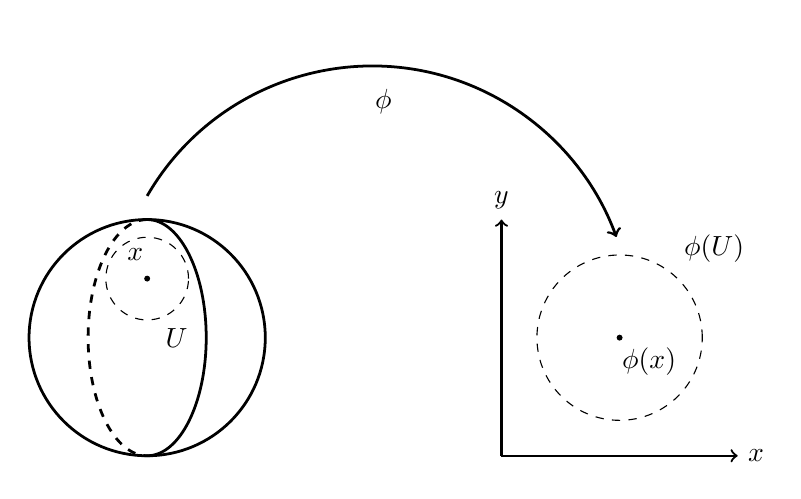
\begin{tikzpicture}[scale=1.5]
  \draw[line width=1] (-3,2) arc (90:-90:0.5 and 1);
  \draw[line width=1, dashed] (-3,2) arc (90:270:0.5 and 1);
  \draw[line width=1](-3,1) circle (1);
  \draw[color=black,thick,->] (0,0) -- (2,0) node[anchor=west]{$x$};
  \draw[color=black,thick,->] (0,0) -- (0,2) node[anchor=south]{$y$};

  \filldraw[black] (1,1) circle (0.02);
  \draw[dashed] (1,1) circle (0.7);
  \draw node at (1.25,0.80) {$\phi(x)$};
  \draw node at (1.8,1.75) {$\phi(U)$};

  \filldraw[black] (-3,1.5) circle (0.02);
  \draw node at (-3.1,1.70) {$x$};
  \draw[dashed] (-3,1.5) circle (0.35);
  \draw node at (-2.75,1) {$U$};

  \draw[line width=1, ->] (-3,2.2) arc (150:20:2.2);
  \draw node at (-1,3) {$\phi$};
\end{tikzpicture}

		\caption{Representación de un homeomorfismo de una variedad a $\R^{2}$.}
	\end{center}
\end{figure}

La definición que acabamos de dar no es única, en el sentido de que existen diferentes definiciones de lo que es una variedad, algunos autores debilitan algunas de las propiedades, por ejemplo, pidiendo que las variedades sean localmente Hausdorff, otros no piden que sean segundo numerables, y algunos otros piden que el homeomorfismo sea con una vecindad abierta de algún espacio de Banach.

Las propiedades que nosotros pedimos, como iremos viendo a lo largo de esta tesis, son bastante agradables para hacer cálculos, ya que, entre otras cosas, nos permitirán extender de manera sencilla funciones locales a toda la variedad y, eventualmente, definir esta propiedad nos permitirá definir lo que es una variedad Riemanniana.


\begin{example}[Espacios Euclidianos]\label{Ex: Variedad Topologica - Espacios Euclidianos}
	El ejemplo más sencillo de una variedad topológica es $(\R^n,d)$ donde $d$ es la función distancia usual.
	\begin{enumerate}
		\item Sabemos que es Hausdorff ya que para cualesquiera dos puntos $x_1,x_2 \in \R^n$ podemos considerar vecindades $V_r(x_1), V_r(x_2)$ donde $r < \frac{d(x,y)}{2}$ de modo que $V_r(x_1) \cap V_r(x_2) = \varnothing$.
		\item Es segundo numerable ya que las bolas abiertas con radios racionales y centros racionales forman una base numerable para la topología.
		\item Para cada $x \in \R^n$ podemos considerar a $\R^n$ como la vecindad abierta y tomar la función identidad $\id: \R^n \to \R^n$ que, trivialmente, es un homeomorfismo.
	\end{enumerate}
\end{example}

\begin{figure}[h]
	\centering
	\begin{tikzpicture}[scale=2]
	\draw[<->] (-2.5,0) -- (-1,0) node[right=3.5pt, below=-1.5pt, font=\fontsize{5pt}{5pt}]{$x$};
	\draw[<->] (-2,-0.5) -- (-2,1) node[above=3pt, font=\fontsize{6pt}{6pt}]{$y$};

	\node[black,font=\fontsize{8pt}{8pt}] at (-1.15,0.85) {$\mathbb{R}^2$};

	\draw[<->] (-0.25,0,0) -- (1.5,0,0) node[above=1pt, font=\fontsize{6pt}{6pt}]{$x$};
	\draw[<->] (0.5,-0.5,0) -- (0.5,1,0)
	node[above=3pt, font=\fontsize{6pt}{6pt}]{$y$};
	\draw[<->] (0.5,0,-1.25) -- (0.5,0,1.25) node[below=3pt,right, font=\fontsize{6pt}{6pt}]{$z$};

	\node[black, font=\fontsize{8pt}{8pt}] at (1.5,0.85) {$\mathbb{R}^3$};
\end{tikzpicture}

	\caption{$\R^2$ y $\R^3$ son variedades topológicas.}
\end{figure}

\begin{example}[Bolas Abiertas]\label{Ex: Variedad Topologica - Bolas Abiertas}
	Otro ejemplo sencillo de variedad topológica son las bolas abiertas en $(\R^n,d)$, donde nuevamente $d$ es la función distancia usual. La topología inducida en la bola hereda el ser Hausdorff y la segundo numerabilidad. Sin pérdida de generalidad podemos suponer que la bola está centrada en el origen y tomarla como la vecindad abierta, así podremos tomar la función $\phi: B_r(0) \to \R^n$ definida por:
	\[
		\phi(x) = \frac{x}{r - \|x\|}.
	\]

	Esta función tiene como inversa a la función $\phi^{-1}: \R^n \to B_r(0)$ dada por:
	\[ \phi^{-1}(y) = \frac{ry}{1 + \|y\|}.
	\]
  Dado que la función inversa existe, $\phi$ es necesariamente una biyección y como ambas funciones son diferenciables serán continuas, por lo que $\phi$ es un homeomorfismo de $B_r(0)$ sobre $\R^n$. Por lo tanto, cualquier bola abierta centrada en el origen será una variedad topológica. Existe un homeomorfismo natural entre una bola arbitraria en $\R^n$ y la bola unitaria en $\R^n$, por lo cual cualquier bola abierta en $\R^n$ será una variedad topológica.
\end{example}

\begin{figure}[h]
	\centering
	\begin{tikzpicture}[scale=4.5]
{\draw[color=black,thick,->] (0,0) -- (1,0) node[anchor=west]{$x$};}%
{\draw[color=black,thick,->] (0,0) -- (0,1) node[anchor=south]{$y$};}%
\draw[dashed] (0.5,0.5) circle (0.25);
\filldraw[black] (0.5,0.5) circle (0.02);
\end{tikzpicture}

	\caption{Una bola abierta en $\R^{2}$ es una variedad topológica.}
\end{figure}


\begin{definition}[Cartas Coordenadas]\label{Definición: Cartas Coordenadas}
	Sea $M^n$ una variedad topológica. Una \it{carta coordenada} en $M$ es un par $(U, \phi)$, donde $U$ es un subconjunto abierto de $M$ y $\phi: U \to \tilde{U}$ es un homeomorfismo de $U$ a un subconjunto abierto $\tilde{U} \subset \R^n$.
\end{definition}

Por definición de variedad topológica cada punto está contenido en el dominio de alguna carta. Dada un carta $(U,\phi)$ llamamos al conjunto $U$ el \it{dominio coordenado}, además, si $\phi(U)$ es una bola abierta en $\R^n$ llamaremos a $U$ una \it{bola coordinada}. Al homeomorfismo $\phi$ se le llama el \it{mapa coordenado (local)}, y a sus funciones componentes $(x^1,\hdots,x^n)$, definidas por $\phi(p) = (x^1(p), \hdots, x^n(p))$ se les conoce como las \it{coordenadas locales} en $U$.

Diremos que una carta $(U,\phi)$ está centrada en un punto $p \in M$ si se cumple que $\phi^{-1}(0) = p$. Geométricamente esto significa que la preimagen del punto $\{0\} \in \R^{n}$ es el punto $p$. Siempre podemos encontrar una carta centrada en $p$ ya que a la imagen de cualquier carta se le puede restar una constante.

A continuación veremos algunos ejemplos más interesantes de variedades topológicas.

\begin{example}[$n-$Esfera]\label{Ex: Variedad Topologica - Esfera}
	La $n-$esfera unitaria, denotada como $\S^n$, y definida como el conjunto:
	\[
		\S^n = \{x \in \R^{n+1}: \| x \| = 1 \}
	\]
	es una variedad topológica.

	En efecto, por ser un subespacio topológico de $\R^{n+1}$ la topología de subespacio de $\S^n$ heredará el ser Hausdorff y segundo numerable.

	Para mostrar que $\S^n$ es localmente euclidiana utilizaremos su proyección sobre el hiperplano $\R^{n}$. Para cada índice $i=1, \hdots, n+1$ definiremos los siguientes subconjuntos de $\S^n$:
	\begin{align*}
		U_{i}^{+} & = \{(x_1,\hdots,x_{n+1}) \in \R^{n+1}: x^i > 0\}, \\
		U_{i}^{-} & = \{(x_1,\hdots,x_{n+1}) \in \R^{n+1}: x^i < 0\}.
	\end{align*}

	Notemos que tendremos $2n + 2$ de estos subconjuntos de $\S^n$ y que estos cubrirán a $\S^n$. Sean $\pi_i: \R^{n+1} \to \R^n$ las funciones proyección que omiten la $i-$ésima coordenada, esto es,
	\[
		\pi_i(x_1,\hdots,x_i,\hdots,x_{n+1}) = (x_1,\hdots,x_{i-1},x_{i+1}\hdots,x_{n+1}).
	\]

	La imagen de cualquier conjunto $U_{i}^{\pm}$ bajo $\pi_i$ será un subconjunto de la bola unidad $\B^n$ en $\R^n$, esto dado que para cualquier $x=(x_1, \hdots, x_{n+1}) \in U_{i}^{\pm}$ se tiene que
	\[
		\|\pi_i(x)\| = \sqrt{\sum_{j=1, j\neq i}^{n+1} x_j^2} < \sqrt{\sum_{j=1}^{n+1} x_j^2} = 1.
	\]

	Ahora definamos funciones $\phi_i^{\pm}: \B^n \to \R^{n+1}$ como sigue, para cada $y=(y_1, \dots, \hat{y_i}, \dots, y_n) \in \B^n$, donde $\hat{y_i}$ significa que no estamos considerando el $i-$ésimo termino:
	\[
		\phi_{i}^{\pm}(y_1, \hdots, y_n) =  (y_1, \hdots, y_{i-1}, \pm\sqrt{1 - \|y\|^2}, y_{i+1}, \hdots, y_{n+1}).
	\]

	Dado que $\|y\| < 1$ la función estará bien definida para cada $y \in \B^n$ y además:
	\begin{align*}
		\|\phi_i^{\pm}(y)\| & = (1 + \| y \|^{2}) + \sum_{\substack{j=1, \\ j \neq i}}^{n+1} y_j^2 \\
		                    & = \left(
		1 - \sum_{\substack{j=1,                                         \\ j \neq i}}^{n+1} y_j^2
		\right) + \sum_{\substack{j=1,                                   \\ j \neq i}}^{n+1} y_j^2 \\
		                    & = 1.
	\end{align*}

	Por lo que $\phi_i^{\pm}(\B^n) \subset U_{i}^{\pm}$. Si ahora consideramos las restricciones $\tau_i^{\pm} = \pi_i |_{U_i^{\pm}}: U_i^{\pm} \to \B^n$ tendremos que $\tau_i^{\pm} \circ \phi_i^{\pm} = \id_{\B^n}$ y $\phi_i^{\pm} \circ \tau_i^{\pm} = \id_{U_i^{\pm}}$. Esto demostraría que existe una biyección entre cada uno de los conjuntos $U_i^{\pm}$ y la bola unidad $\B^n$ en $\R^n$, además de esto, tanto $\tau_i^{\pm}$ como $\phi_i^{\pm}$ son funciones continuas por lo que serán homeomorfismos, y, como cada $x \in S^n$ está contenido en algún $U_i^{\pm}$, concluimos que $\S^n$ es una variedad topológica de dimensión $n$.
\end{example}

\begin{figure}[h!]
	\centering
	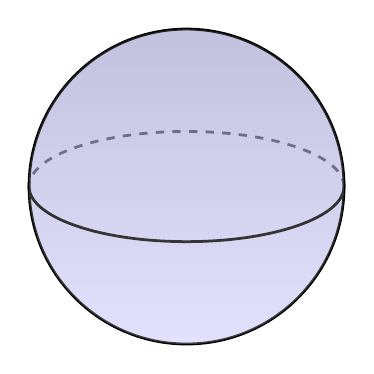
\begin{tikzpicture}[scale=2]
  \draw[line width=1, dashed] (1,0) arc (0:180:1 and 0.35);
  \draw[fill=blue!30!white!,opacity=0.5] (0,0) circle (1);
  \draw[line width=1] (1,0) arc (0:180:1 and -0.35);
  \draw[line width=1](0,0) circle (1);
  \shade[opacity=0.25] (0,0) circle (1);
\end{tikzpicture}


	\caption{La esfera $\S^{2}$ es una variedad topológica.}
\end{figure}

\begin{example}[Producto Finito de Variedades]\label{Ex: Variedad Topologica - Producto de Variedades}
	Si $M_1, \hdots, M_k$ son variedades topológicas de dimensiones $n_1,\hdots,n_k$ respectivamente, entonces $M = \Pi_{i=1}^k M_i$ es una variedad topológica de dimensión $\sum_{i=1}^k n_i$.

	En efecto, comencemos considerando el caso del producto de dos variedades. Sean $M_{1}^{n_1}$ y $M_{2}^{n_2}$ variedades topológicas. Como el producto arbitrario de espacios de Hausdorff es Hausdorff, tendremos que $M_1 \times M_2$ es Hausdorff. Además, como el producto numerable de espacios segundo numerables es segundo numerable $M_1 \times M_2$ es segundo numerable.
	Para cada punto $(x,y) \in M_1 \times M_2$ existirá un conjunto abierto $U \times V$ donde $U$ es el dominio de una carta $(U,\phi)$ en $M_1$ que contiene que a $x$ y $V$ es el dominio de una carta $(V,\psi)$ que contiene a $y$, por definición de cartas coordenadas $\phi: U \to \R^{n_1}$ y $\psi: V \to \R^{n_2}$ son homeomorfismo, por lo que podemos definir la función $F: U \times V \to \R^{n_1 + n_2}$ como:
	\[
		F(x,y) = (\phi(x),\psi(y)).
	\]

	Dado que $\phi$ y $\psi$ son homeomorfismo en particular serán funciones continuas, por lo que podemos garantizar que $F$ es continua y además es invertible, en particular, su inversa estará dada por $F^{-1}(a,b) = (\phi^{-1}(a),\psi^{-1}(b))$ y como las inversas de $\phi$  y $\psi$ también son continuas $F^{-1}$ es un mapa continuo. Así, $F$ es un homeomorfismo de $U \times V$ sobre $\R^{n_1 + n_2}$, como esto se cumple para cada punto $(x,y) \in M_1 \times M_2$ podemos concluir que el producto $M_1 \times M_2$ es una variedad topológica.

	El caso para el producto finito de variedades topológicas se sigue por inducción.
\end{example}

\begin{example}[$n-$Toro]\label{Ex: Variedad Topologica - Toro}
	El toro $n$-dimensional, que se denota por $\T^n$, y que se define como:
	\[
		\T^n = \underbrace{\S^1 \times \hdots \times \S^1}_{n-\text{veces}}.
	\]

	Esto se puede ver a partir de los ejemplos \ref{Ex: Variedad Topologica - Esfera} y \ref{Ex: Variedad Topologica - Producto de Variedades}, ya que son el producto finito de variedades topológicas.
\end{example}

\begin{figure}[h]
	\centering
	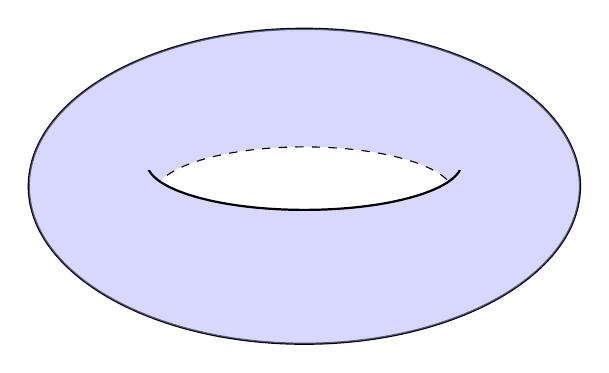
\begin{tikzpicture}[scale=2]
  % Elipse Principal
	\draw [thick] (0,0) ellipse  (1.75 and 1);
	\path[fill=blue!30!white,opacity=0.5] (0,0) ellipse  (1.75 and 1);

	%Arco inferior
	\begin{scope}
		\clip (0,0.15) ellipse (1 and 0.3);
		\fill[white] (0,-0.05) ellipse (0.95 and 0.3);
	\end{scope}

	% Arco superior
	\begin{scope}
		\clip (-1.25,0.03) rectangle (1.25,0.5);
		\draw[dashed] (0,-0.05) ellipse (0.95 and 0.3);
	\end{scope}

  % Centro
	\begin{scope}
		\clip (-1.25,0.1) rectangle (1.25,-0.5);
		\draw[thick] (0,0.15) ellipse (1 and 0.3);
	\end{scope}
\end{tikzpicture}

	\caption{El toro $\mathbb{T}^{2}$ es una variedad topológica.}
\end{figure}

% \cleardoublepage
% \section{Variedades Suaves}\label{Sección: Variedades Suaves}
Las variedades topológicas tienen propiedades muy interesantes en sí mismas, sin embargo, para nuestros fines lo que nos interesa es poder realizar cálculos en ellas, en particular darle sentido a la noción de diferenciabilidad. Esto no es posible en general, es con este fin que daremos algunas definiciones que nos permitirán construir una estructura adicional con la cual podremos dotar a algunas variedades topológicas; esta estructura será lo que nos permitirá dar sentido a la derivada.

Cuando decimos que una función $f$ es diferenciable o suave lo que queremos decir es que: Si $U$ y $V$ son subconjuntos abiertos de $\R^n$ y $\R^m$ respectivamente, entonces  $f: U \to V$ tiene derivadas parciales de todos los órdenes. Al conjunto de funciones con esta propiedad usualmente se le denota como $C^{\infty}$ y se dice que las funciones son de clase $C^{\infty}$.


\begin{definition}[Mapa de Transición]\label{Definición: Mapa de Transición}
	Sea $M^n$ una variedad topológica y $(U,\phi)$, $(V,\psi)$ cartas en $M$. Si $U \cap V \neq \varnothing$, entonces a la composición $\psi \circ \phi^{-1}: \phi(U \cap V) \to \psi(U \cap V)$ es llamada el \it{mapa de transición de $\phi$ a $\psi$}
\end{definition}

\begin{definition}[Cartas Suavemente Compatibles]\label{Definición: Cartas Suavemente Compatibles}
	Diremos que dos cartas $(U,\phi)$ y $(V,\psi)$ son \it{suavemente compatibles} o $C^{\infty}-$compatibles si $U \cap V = \varnothing$ o si los mapas de transición
	\[ \psi \circ \phi^{-1}: \phi(U \cap V) \to \psi(U \cap V), \quad \phi \circ \psi^{-1}: \psi(U \cap V) \to \phi(U \cap V) \]
	son ambos suaves.
\end{definition}

\begin{figure}[h]
	\centering
	\begin{tikzpicture}[scale=1]
	\coordinate (a) at (0,0);
	\path[draw,use Hobby shortcut,closed=true,thick]
	(0,2.5) .. (2,2.5) .. (1,4.5) .. (.3,4.5) .. (-1,4) .. (-2,2.5);

	\begin{scope}
		\clip (0.25,3.5) circle (0.5);
		\fill[blue!30!white,opacity=0.5] (-0.25,3.25) circle (0.5);
	\end{scope}
	\draw[dashed] (0.25,3.5) circle (0.5);
	\draw[dashed] (-0.25,3.25) circle (0.5);
	\draw node at (0.8,4) {$V$};
	\draw node at (-0.9,2.75) {$U$};

	\draw [thick, <->] (-5,0) -- (-1,0);
	\draw [thick, <->] (-3,-2) -- (-3,2);
	\draw [thick, <->] (1,0) -- (5,0);
	\draw [thick, <->] (3,-2) -- (3,2);

	\begin{scope}
		\clip (-3,0.5) ellipse  (0.8 and 1);
    \fill[color=blue!30!white,opacity=0.5] (-2.5,0) ellipse  (1.2 and 0.8);
	\end{scope}
	\draw [dashed,thick] (-3,0.5) ellipse  (0.8 and 1);
	% \draw [dashed,thick] (-2.5,0) ellipse  (1.2 and 0.8);

	\begin{scope}
		\clip (3,0.5) ellipse  (0.8 and 1);
		\fill[color=blue!30!white,opacity=0.5](3.5,0) ellipse  (1.2 and 0.8);
	\end{scope}
	% \draw [dashed,thick] (3,0.5) ellipse  (0.8 and 1);
	\draw [dashed,thick] (3.5,0) ellipse  (1.2 and 0.8);

	\draw[line width=1, ->] (1,3.75) arc (90:-5:2.5);
	\draw[line width=1, ->] (-1,3.25) arc (-90:0:-1.5);
	\draw[line width=1, ->] (-1.75,0.5) -- (2,0.5);

	\draw node at (-2.5,2.75) {$\phi$};
	\draw node at (3.25,3) {$\psi$};
	\draw node at (-4.25,1.25) {$\phi(U)$};
	\draw node at (4.5,1) {$\psi(V)$};
	\draw node at (0.25,1) {$\psi \circ \phi^{-1}$};


\end{tikzpicture}

	\caption{Mapa de Transición}
\end{figure}

Verificar que dos cartas son suavemente compatibles es relativamente sencillo, dado que el mapa de transición es una composición de homeomorfismos este será un homeomorfismo, así, únicamente habrá que verificar que la función y su inversa son diferenciables.

\begin{definition}[Atlas, Atlas Suave y Atlas Maximal]\label{Definición: Atlas}
	Sea $M$ una variedad topológica. Un \it{atlas} en $M$, denotado como $\A$, es una colección indexada $\{(U_i,\phi_i)\}_{i\in I}$ de cartas en $M$ que cubren a la variedad, esto es:
	\[\bigcup_{i \in I} U_i = M \]

	Si cualesquiera dos cartas en un atlas son suavemente compatibles, entonces diremos que el atlas es un \it{atlas suave}. A las cartas que forman a un atlas suave se les llama \it{cartas suaves}.

	Un atlas $\A$ estará contenido en otro atlas $\mathcal{B}$ si cada carta $(U,\phi)$ que pertenece a $\A$ también pertenece a $\mathcal{B}$. Diremos que un atlas suave $\A$ es \it{maximal} si no está propiamente contenido en ningún atlas más grande.
\end{definition}

\begin{definition}[Variedad Suave]\label{Definición: Variedad Suave}
	Sea $M$ una variedad topológica. Una \it{variedad suave} será un par $(M, \A)$, donde $\A$ es un atlas maximal en $M$. Usualmente a $\A$ se le llama la \it{estructura suave} en $M$.
\end{definition}

Por conveniencia, en lugar de escribir \enquote{Sea $(M,\A)$ una variedad suave} diremos simplemente \enquote{Sea $M$ una variedad suave}; esto cuando la estructura suave se pueda entender a partir del contexto o no sea necesario referirnos a ella de forma explícita.


Si quisiéramos definir una función $f: M \to \R$ como suave, quizá pudiésemos haber estado inclinados a dar la siguiente definición: \enquote{Una función $f: M \to \R$ es diferenciable si y sólo si para cada carta $(U,\phi)$ se tiene que $f\circ \phi^{-1}: \phi(U) \to \R$ es una función diferenciable}, esta definición podría parecernos más natural, sin embargo, presenta un problema de ambigüedad ya que, para una misma variedad pueden existir muchos atlas diferentes que generan estructuras similares pero distintas, como veremos en los siguientes ejemplos.

\begin{figure}[h]
	\begin{center}
		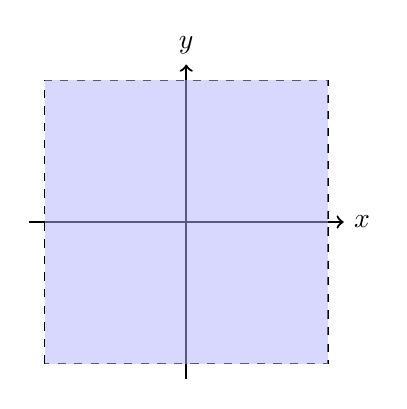
\begin{tikzpicture}[scale=2, baseline={(0,-1.5)}]
\draw[color=black,thick,->] (-1,0) -- (1,0) node[anchor=west]{$x$};%
\draw[color=black,thick,->] (0,-1) -- (0,1) node[anchor=south]{$y$};%

\draw[dashed] (-0.90,-0.90) rectangle (0.90,0.90);
\path[fill=blue!30!white,opacity=0.5] (-0.90,-0.90) rectangle (0.90,0.90);

\end{tikzpicture}

		\caption{Representación de $\R^2$ siendo cubierta por una única carta.}
	\end{center}
\end{figure}

\begin{example}[Variedades Cubiertas Por Una Única Carta]\label{Ex: Variedad Suave - Carta Unica}
	Si $M^n$ es una variedad topológica y existe un atlas para $M$ que contiene a una única carta entonces la carta define una estructura suave para la variedad, esto dado que trivialmente cumplirá el ser suavemente compatible con cualquier otra carta en el atlas.
\end{example}


\begin{example}[Espacios Euclidianos]\label{Ex: Variedad Suave - Espacios Euclidianos}
	Si tomamos cualquier espacio Euclidiano $\R^n$ podemos dar el atlas formado únicamente por la carta $(\R^n,\id_{\R^n})$, por el ejemplo anterior sabemos que esta carta define una estructura suave en $\R^n$.
\end{example}

\begin{example} % Ejemplo de diferentes estructuras suaves.
	Podemos considerar la función $\psi: \R \to \R$, definida del siguiente modo:
	\[
		\psi(x) = x^3
	\]

	Esta función es un homeomorfismo, y por los ejemplos anteriores sabemos que $(\R, \psi(x))$ es una variedad suave, con la estructura definida por  $\psi$. Sin embargo, al considerar el mapa de transición tenemos que $\id_{\R} \circ \psi^{-1}(y) = y^{\frac{1}{3}}$, y esta función no es diferenciable en el origen, por lo cual las cartas no son suavemente compatibles, y las estructuras determinadas por $(\R, \id_{\R})$ y $(\R,\psi)$ serán diferentes.
\end{example}

Para resolver este problema de ambigüedad es que hemos introducido el concepto atlas maximal. Lo que el atlas maximal nos garantiza es que cada carta que sea suavemente compatible con cualquier otra carta en el atlas estará ya incluida en el mismo.

\begin{theorem}
	Si $M$ es una variedad topológica, entonces cada atlas suave $\A$ de $M$ está contenido en un atlas suave maximal único, llamado la \it{estructura suave determinada por $\A$}.
\end{theorem}

\begin{proof}
	Sea $\A$ un atlas suave para $M$ y sea $\bar{\A}$ el conjunto de todas las cartas que son suavemente compatibles con todas las cartas de $\A$.
	\begin{enumerate}
		\item $\bar{A}$ es un atlas suave. Consideremos dos cartas arbitrarias $(U,\phi)$ y $(V,\psi)$ en $\bar{\A}$, además consideremos un punto arbitrario $\phi(p) \in \phi(U \cap V)$. Por definición el atlas $\A$ cubre a $M$, por lo que existirá una carta $(W,\theta)$ en $\bar{A}$ tal que $p \in W$, por construcción de $\bar{A}$ sabemos que $\psi \circ \theta^{-1}$ y $\theta \circ \phi^{-1}$ son suaves. Y, dado que $p \in U \cap V \cap W$, se sigue que $\psi \circ \phi^{-1} = (\psi \circ \theta^{-1}) \circ \theta \circ \phi^{-1}$, al ser una composición de funciones suaves será suave en $\phi(U \cap V)$, dado que hemos elegido las cartas $(U,\phi)$ y $(V,\psi)$ de manera arbitraria podemos concluir que $\bar{\A}$ es un atlas suave.
		\item $\bar{\A}$ es un atlas maximal. Si consideramos una carta que sea suavemente compatible con cualquier otra carta en $\bar{\A}$ por construcción esta carta deberá ser suavemente compatible con cualquier otra carta en $\A$, pero esto implica que la carta pertenece a $\bar{\A}$, por lo tanto $\bar{\A}$ es maximal.
		\item $\bar{\A}$ es único. Tomando algún otro atlas suave maximal $\mathcal{B}$ que contenga a $\A$ tendremos que cada una de sus cartas es suavemente compatible con cada carta en $\A$ por lo que $\mathcal{B} \subseteq \bar{\A}$, pero al ser $\mathcal{B}$ maximal se tendrá que $\mathcal{B} = \bar{A}$
	\end{enumerate}
\end{proof}

\begin{theorem}\label{Teorema: Unicidad de Estructura Suave}
	Dos atlas suaves para una variedad $M$ determinan la misma estructura suave si y sólo si su unión es un atlas suave.
\end{theorem}

\begin{proof}
	Sean $\A$ y $\mathcal{B}$ dos atlas suaves en $M$ y que ambos determinan la misma estructura suave. Por el teorema anterior sabemos que esto significa que existe un atlas suave maximal $\mathcal{C}$ tal que $\A \subset \mathcal{C}$ y $\mathcal{B} \subset \mathcal{C}$.

	Si consideramos una carta $(U,\phi) \in \A \cup \mathcal{B}$ esta deberá estar contenida en $\A$ o $\mathcal{B}$, podemos suponer sin pérdida de generalidad que está contenida en $\A$, también estará contenida en $\mathcal{C}$ y por construcción cada carta en $\mathcal{C}$ debe ser suavemente compatible con cada carta en $\mathcal{B}$, análogamente para el caso en que la carta está contenida en $\mathcal{B}$. Por lo tanto, podemos concluir que $\A \cup \mathcal{B}$ es un atlas suave.

	Supongamos ahora que $\A \cup \mathcal{B}$ es un atlas suave. Dado que las estructuras suaves determinadas por $\A$ y $\mathcal{B}$ ambas contendrán a $\A \cup \mathcal{B}$, y que por el teorema anterior hay una única estructura suave que contiene a $\A \cup \mathcal{B}$ podemos concluir que $\A$ y $\mathcal{B}$ determinan la misma estructura suave.
\end{proof}

Lo que estos dos teoremas nos permiten hacer es definir de manera más sencilla la estructura suave para una variedad, ya que, en lugar de tener que describir un atlas maximal podemos simplemente escoger algún atlas suave y sabemos que la estructura determinada será única.

Hay muchos ejemplos de variedad suaves y, como veremos a continuación, a cada una de las variedades topológicas que dimos como ejemplo anteriormente se le puede dar una estructura suave, sin embargo, esto no es cierto en general, hay ejemplos de variedades topológicas a las cuales no se les puede dar una estructura suave. Un resultado interesante que no veremos aquí es que, si $M^n$ es una variedad topológica con $n=1,2,3$, entonces a esta se le puede dar una estructura suave, esto fue probado por James Munkres en 1960, la demostración puede ser consultada en \enquote{\textcite{munkres1960obstructions}}.


\begin{example}[Espacios Vectoriales Finito-Dimensionales]\label{Ex: Variedad Sauve - Espacios Vectoriales}
	Sea $V$ un espacio vectorial real finito dimensional. Sabemos que todo espacio vectorial tiene una base, supongamos que $\{x_1,\dots,x_n\}$ es dicha base. Existe un isomorfismo lineal canónico $\phi: V \to \R^n$ dado por:
	\[ \phi(a_1 x_1 + \dots + a_n x_n) = (a_1, \dots, a_n) \]
	Es posible definir una métrica en $V$, la cual podemos definir del siguiente modo:
	\[d(x,y) = \|x - y\|\]

    Esta métrica nos inducirá una topología, la cual hará de nuestro isomorfismo entre espacios vectoriales un homeomorfismo lineal entre espacios topológicos.

	Al considerar algún otro homeomorfismo lineal $\psi: V \to \R^n$ se tendrá que la composición $\psi \circ \phi^{-1}: \phi(V) \to \R^n$ también es un homeomorfismo, por lo que tanto $\psi$ como $\phi$ determinan la misma topología en $V$. Al ser $\phi$ un homeomorfismo podemos garantizar que $V$ es Hausdorff y segundo numerable. Así, cada espacio vectorial real finito dimensional es una variedad topológica.

	Podemos considerar el atlas formado por la carta $(V,\phi)$, donde $\phi$ es algún homeomorfismo lineal de $V$ a $\R^n$, por el ejemplo \ref{Ex: Variedad Suave - Carta Unica} que esta carta determinará una estructura suave para $V$.
\end{example}

\begin{example}[Subconjuntos Abiertos De Variedades Suaves]\label{Ex: Variedad Suave - Subvariedades Suaves}
	Sea $M^n$ una variedad suave y $U$ un subconjunto abierto de $M$, entonces $U$ es una variedad suave.

	De modo similar al ejemplo \ref{Ex: Variedad Topologica - Bolas Abiertas} podemos mostrar que en general los subconjuntos abiertos de las variedades topológicas son, en sí mismos, variedades topológicas.

	Si $M$ es una variedad topológica y $U \subset M$ es abierto, entonces la topología inducida en $U$ heredará el ser Hausdorff y segundo numerable. Cada punto en $U$ está contenido en una carta de la variedad; dicha carta restringida a $U$ y el mapa coordenado nos da un homeomorfismo entre $U$ y algún conjunto abierto en $\R^n$, por lo que $U$ es una variedad topológica. Usualmente cuando hablamos de un subconjunto abierto de una variedad para enfatizar nos referiremos a él como una \it{subvariedad abierta}.

	Dado que $M$ es una variedad suave, existirá un atlas maximal $\A = \{(V_i,\phi_i) \}_{i \in I}$ en $M$, para cualquier conjunto abierto $U$ de $M$ podemos considerar el atlas:
	\[ \A_U = \{(V_i \cap U, \phi_i |_{V_i \cap U})\}_{i \in I} \]

	Como cada una de las cartas en $\A$ es suavemente compatible con cualquier otra carta en $\A$, sus restricciones a $V_i \cap U$ también serán suavemente compatible con cualquier otra carta en $\A$, en particular con aquellas restringidas a $V_i \cap U$. Por lo tanto $(U, \A_U)$ será una variedad suave.
\end{example}

\begin{example}[$n-$Esfera]
	La $n$-esfera $\S^n$ es una variedad suave.

	\begin{figure}[h]
		\begin{center}
			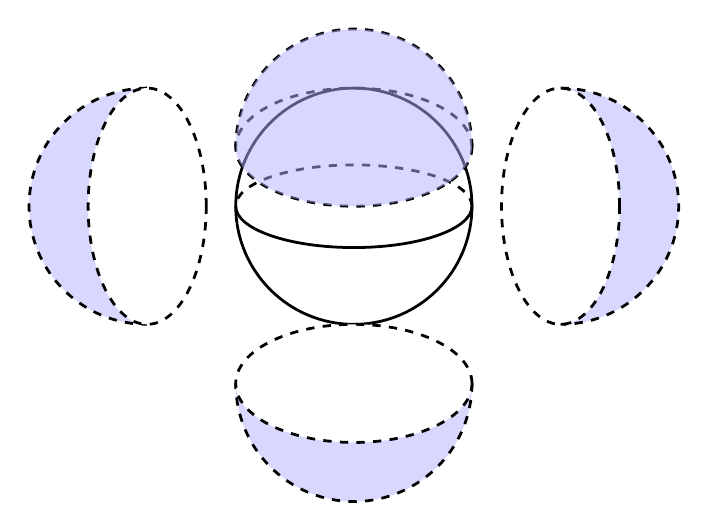
\begin{tikzpicture}[scale=1.5]
  \draw[line width=1, dashed] (1,0) arc (0:180:1 and 0.35);
  \draw[line width=1] (1,0) arc (0:180:1 and -0.35);
  \draw[line width=1](0,0) circle (1);

  % Left Chart
  \path[fill=blue!30!white,opacity=0.5] (-1.75,1) arc (90:-90:-1 and 1);
  \draw[line width=1, dashed] (-1.75,1) arc (90:-90:-1 and 1);
  \draw[fill=white, line width=1, dashed] (-1.75,0) ellipse (0.5 and 1);

  % Right Chart
  \path[fill=blue!30!white,opacity=0.5,line width=1, dashed] (1.75,1) arc (90:-90:1 and 1);
  \draw[fill=white, line width=1, dashed] (1.75,0) ellipse (0.5 and 1);
  \draw[line width=1, dashed] (1.75,1) arc (90:-90:1 and 1);

  % Top Chart
  \draw[line width=1, dashed] (0,0.5) ellipse (1 and 0.5);
  \draw[line width=1, dashed] (1,0.5) arc (0:180:1 and 1);
  \path[fill=blue!30!white,opacity=0.5] (1,0.5) arc (0:-180:1 and 0.5);
  \path[fill=blue!30!white,opacity=0.5] (1,0.5) arc (0:180:1 and 1);


  % Bottom Chart
  \path[fill=blue!30!white,opacity=0.5,line width=1, dashed] (1,-1.5) arc (0:-180:1 and 1);
  \draw[line width=1, dashed] (1,-1.5) arc (0:-180:1 and 1);
  \draw[fill=white, line width=1, dashed] (0,-1.5) ellipse (1 and 0.5);
\end{tikzpicture}

			\caption{Representación de cuatro de las seis cartas suaves con las que cubrimos a la $2-$esfera.}
		\end{center}
	\end{figure}

	Si consideramos los conjuntos de cartas que $\{(U_i^{\pm}, \phi_{i}^{\pm})\}_{i=1}^{n}$ y las inversas de estas funciones se definen en el ejemplo \ref{Ex: Variedad Topologica - Esfera}. Para cualesquiera dos cartas se tendrán dos casos, los índices $i,j$ son iguales o son diferentes. En el caso en que los índices son iguales se tiene que el mapa de transición es:

	\[ \phi_i^{+} \circ \left(\phi_{i}^{-}\right)^{-1} = \phi_i^{-} \circ \left(\phi_{i}^{+}\right)^{-1} = \id_{\B^n} \]
	En el caso en el que los índices son diferentes tendremos que el mapa de transición está dado como:
	\[ \phi_i^{+} \circ \left(\phi_{j}^{-}\right)^{-1}(u_1, \dots, u_n) = \left(u_1, \dots, \underbrace{\pm \sqrt{1 - \|u\|^2}}_{j-\text{ésimo término}},\dots, u_{i-1}, u_{i+1}, \dots, u_{n} \right) \]

	En ambos casos las composiciones son diferenciables y en ningún punto cero, podemos concluir entonces que ambas son difeomorfismos. Por lo tanto, determinan una estructura suave en $\S^n$.
\end{example}

\begin{example}[Producto Finito de Variedades Suaves]\label{Ex: Variedad Suave - Producto de Variedades Suaves}
	Si $M_1^{n_1},\dots,M_k^{n_k}$ son variedades suaves entonces $M_1 \times \dots \times M_k$ es una variedad suave. Como se hizo en el ejemplo \ref{Ex: Variedad Topologica - Producto de Variedades} procederemos considerando el producto de únicamente dos variedades suaves, el caso para el producto de un número arbitrario pero finito se seguirá por inducción.
	En el ejemplo \ref{Ex: Variedad Topologica - Producto de Variedades} probamos que si $M_1$ y $M_2$ son variedades topológicas con cartas de $(U,\phi)$ y $(V,\psi)$ respectivamente entonces $M_1 \times M_2$ es una variedad topológica y tiene cartas de la forma $(U \times V,\phi \times \psi)$. Si $M_1$ y $M_2$ son variedades suaves y consideramos dos cartas cualesquiera $(U_1 \times V_1, \phi_1 \times \psi_1)$, $(U_2 \times V_2, \phi_2 \times \psi_2)$ de $M_1 \times M_2$ entonces tendremos que el mapa de transición será:
	\[
		(\phi_2 \times \psi_2) \circ (\phi_1 \times \psi_1)^{-1} = (\phi_2 \circ \phi_1^{-1}) \times (\psi_2 \circ \psi_1^{-1})
	\]
	Como $M_1$ y $M_2$ son variedades suaves las cartas $(U_1,\phi_1)$, $(U_2,\phi_2)$, $(V_1,\psi_1)$, $(V_2,\psi_2)$ serán suavemente compatibles. Por lo tanto $M_1 \times M_2$ es una variedad suave.
\end{example}

Es importante no perder de vista que una variedad topológica no es suave en sí misma, la suavidad es una estructura adicional que se le agrega a la variedad a través de la estructura suave. Como se mencionaba anteriormente para una misma variedad pueden existir muchos atlas y muchos de ellos pueden ser atlas suaves o atlas maximales.

Para los ejemplos anteriores se ha mostrado que estas son variedades suaves comenzando con un espacio topológico y luego mostrando que este cumple con la definición de variedad topológica y finalmente ser dotado de una estructura suave. El siguiente lema nos da una alternativa, dándonos una manera de dotar a un conjunto de una estructura topológica y  una estructura suave.

\begin{lemma}\label{Lemma: Lema de Cartas Suaves de una Variedad}
	Sea $M$ un conjunto, $\{U_\alpha\}$ una colección de subconjuntos de $M$ y $\{\phi_\alpha\}$ una colección de mapas donde $\phi_\alpha: U_\alpha \to \R^n$ tales que las siguientes propiedades se cumplen:

	\begin{enumerate}
		\item Para cada $\alpha$, $\phi_\alpha$ es una biyección entre $U_\alpha$ y un subconjunto abierto $\phi_\alpha(U) \subseteq \R^n$.
		\item Para cualesquiera $\alpha, \beta$, los conjuntos $\phi_{\alpha}(U_\alpha \cap U_\beta)$ y $\phi_{\beta}(U_\alpha \cap U_{\beta})$ son ambos abiertos en $\R^n$.
		\item Si $U_\alpha \cap U_\beta \neq \varnothing$, el mapa $\phi_{\beta} \circ \phi_{\alpha}^{-1}: \phi_{\alpha}(U_{\alpha} \cap U_{\beta}) \to \phi_{\beta}(U_{\alpha} \cap U_{\beta})$ es suave.
		\item Existe una cubierta numerable para $M$ formada por elementos de $\{U_\alpha\}$.
		\item Si $p,q \in M$ y $p \neq q$, entonces existe un subconjunto $U_\alpha$ que contiene a $p$ y $q$, o existen subconjuntos disjuntos $U_{\alpha}$ y $U_{\beta}$ tales que $p \in U_{\alpha}$ y $q \in U_{\beta}$.
	\end{enumerate}

	Entonces $M$ tiene una estructura suave única tal que cada $(U_{\alpha},\phi_{\alpha})$ es una carta suave.
\end{lemma}

\begin{proof}
	Comenzaremos definiendo un conjunto el cual probaremos será una base para una topología en $M$. Sea $\mathcal{B}$ el conjunto formado por todos los $\phi_{\alpha}^{-1}(V) \in M$ tales que $V \subseteq \R^n$ es abierto. Por la propiedad 4 se garantiza que una subcolección numerable de $\mathcal{B}$ cubre a $M$, tomemos dos elementos de $\mathcal{B}$, $\phi_{\alpha}^{-1}(V)$ y $\phi_{\beta}^{-1}(W)$ y notemos que las siguientes igualdades se cumplen:
	\begin{align*}
		\phi_{\alpha}^{-1}(V) \cap \phi_{\beta}^{-1}(W) & = \phi_{\alpha}^{-1}(V) \cap (\phi_{\alpha}^{-1} \circ \phi_{\alpha} \circ \phi_{\beta}^{-1})(W)  \\
		                                                & = \phi_{\alpha}^{-1}(V) \cap \phi_{\alpha}^{-1} ((\phi_{\beta} \circ \phi_{\alpha}^{-1})^{-1}(W)) \\
		                                                & = \phi_{\alpha}^{-1} (V \cap (\phi_{\beta} \circ \phi_{\alpha}^{-1})^{-1}(W))
	\end{align*}

	Por la propiedad 3 sabemos que $\phi_{\beta} \circ \phi_{\alpha}^{-1}$ es suave, por lo que en particular será un mapa continuo, luego $(\phi_{\beta} \circ \phi_{\alpha})^{-1}(W)$ será abierto en $\R^n$, dado que será un subconjunto abierto de $\phi_{\alpha}(U_{\alpha} \cap U_{\beta})$ y este es, en sí mismo, un subconjunto abierto de $\R^n$ por la propiedad 2. Por lo propiedad 1 se garantiza que $\phi_{\alpha}^{-1}(V) \cap \phi_{\beta}(W) \in \mathcal{B}$, esto es suficiente para mostrar que $\mathcal{B}$ es una base para $M$.

	Ahora mostraremos que $M$ con la topología dada por la base $\mathcal{B}$ es, en efecto, una variedad topológica.

	Por definición de $\mathcal{B}$ cada $\phi_{\alpha}$ es un homeomorfismo sobre un subconjunto abierto de $\R^n$, por lo tanto, para cada $p \in M$ existirá una vecindad que lo contenga y un homeomorfismo de dicha vecindad sobre todo $\R^n$, esto prueba que $M$ con la topología dada es localmente euclidiano.

	Para mostrar que $M$ es Hausdorff con la topología consideremos $p, q \in M$ tales que $p \neq q$. Por la propiedad 5 solo existirán dos posibilidades, si existen subconjuntos $U_{\alpha}$, $U_{\beta}$ tales que $p \in U_{\alpha}$, $q \in U_{\beta}$ y $U_{\alpha} \cap U_{\beta} \neq \varnothing$ habremos terminado. La segunda posibilidad es que exista $U_{\alpha}$ tal que $p, q \in U_{\alpha}$, dado que $\phi_{\alpha}(U_{\alpha}) \subseteq \R^n$ es un subconjunto abierto existirán subconjuntos $V,W \subset \phi_{\alpha}(U_{\alpha})$ disjuntos tales que $\phi_{\alpha}(p) \in V$ y $\phi_{\alpha}(q) \in W$, por lo que $\phi_{\alpha}^{-1}(V)$ y $\phi_{\alpha}^{-1}$ serán vecindades disjuntas de $p$ y $q$. Por lo tanto $M$ con la topología dada es Hausdorff.

	La segundo numerabilidad de $M$ se tiene del hecho de que $\R^n$ es segundo numerable por lo que cada $\phi_{\alpha}(U_{\alpha})$ será segundo numerable, por ser $\phi_{\alpha}$ un homeomorfismo $U_{\alpha}$ será segundo numerable, y ocupando la propiedad 4 podemos concluir que $M$ es segundo numerable.

	Con esto hemos probado que $M$ es una variedad topológica. Y por la propiedad 3 podemos concluir que cada carta $(U_{\alpha},\phi_{\alpha})$ es una carta suave, por el teorema \ref{Teorema: Unicidad de Estructura Suave} se concluye que la estructura suave determinada por la colección de cartas es única.
\end{proof}

% \cleardoublepage
% \section{Mapas Suaves}\label{Sección: Mapas Suaves}
Habiendo definido las variedades topológicas y las variedades suaves ahora nos interesará estudiar lo que son los mapas suaves, estos son difeomorfismos entre variedades, los difeomorfismos son funciones o mapas bajo los cuales la estructura suave se preserva.

Haremos la siguiente distinción entre los términos \it{función} y \it{mapa}. Una mapa será una regla que a cada elemento de su dominio le asigna un elemento del contradominio, donde, el dominio y contradominio pueden ser variedades arbitrarias, mientras que una función será un tipo particular de mapa donde el contradominio es $\R^n$ para algún $n \in \N$.

\begin{definition}[Funciones Suaves]\label{Definición: Función Suave}
	Sea $M^n$ una variedad suave, $k$ un entero no negativo, y $f: M \to \R^{k}$ una función cualquiera. Diremos que $f$ es una \it{función suave} si para cada punto $p \in M$ existe una carta suave $(U,\phi)$ para $M$, cuyo dominio contiene a $p$ y tal que la composición de las funciones $f \circ \phi^{-1}$ es suave en el conjunto abierto $\phi(U) \subseteq \R^{n}$.
\end{definition}

\begin{figure}[h]
	\centering
	\begin{tikzpicture}[scale=0.85]
  \coordinate (a) at (0,0);
\path[draw,use Hobby shortcut,closed=true,thick]
(0,2.5) .. (2,2.5) .. (1,4.5) .. (.3,4.5) .. (-1,4) .. (-2,2.5);

\draw[dashed] (0.25,3.5) circle (0.6);
\draw node at (0,3.6) {$U$};
\draw node at (-1.5,4.5) {$M$};

\draw [thick, <->] (-5,0) -- (-1,0);
\draw [thick, <->] (-3,-2) -- (-3,2);
\draw [thick, <->] (1,0) -- (5,0);
\draw [thick, <->] (3,-2) -- (3,2);

\draw [dashed,thick] (-3,-0.25) ellipse  (1.5 and 1.2);


\draw[line width=1, ->] (1,3.75) arc (90:0:2.5);
\draw[line width=1, ->] (-0.75,3.5) arc (-90:0:-2);
\draw[line width=1, ->] (-1.5,-1.5) arc (60:120:-3.5);

\draw node at (-2.75,3) {$\phi$};
\draw node at (3.25,3) {$f$};
\draw node at (-2.25,-0.5) {$\phi(U)$};
\draw node at (-4.5,1) {$\R^n$};
\draw node at (4.5,1) {$\R^{k}$};
\draw node at (0.5,-1.25) {$f \circ \phi^{-1}$};
\end{tikzpicture}

	\caption{Representación de una función suave.}
\end{figure}

Notemos que en el caso en que la variedad que consideramos es $M = \R^n$ o algún subconjunto abierto de $\R^n$, la definición anterior coincide con la definición de cálculo multivariable ya que, como se vio en el ejemplo \ref{Ex: Variedad Suave - Espacios Euclidianos}, $\R^n$ es una variedad suave con la estructura suave dada por $(\R^n,\id_{\R^n})$ y al componer cualquier función con la identidad obtendremos la misma función.

Uno de los casos más importantes de las funciones suaves son aquellas que van de la variedad a los números reales, esto es, funciones suaves $f: M \to \R$. Al conjunto formado por estas funciones se le denota por $C^{\infty}(M)$, este es un espacio vectorial dado que la suma de funciones suaves y el producto de un escalar por una función suave son funciones suaves.

Podemos generalizar todavía más la noción de función suave si en lugar de restringirnos a $\R^k$ como el contradominio de las funciones dejamos que el contradominio sea cualquier variedad, esto se logra de la siguiente manera.

\begin{definition}[Mapa Suave]\label{Definición: Mapa Suave}
	Sean $M^{k_1}$ y $N^{k_2}$ variedades suaves, y sea $f: M \to N$ un mapa cualquiera. Diremos que $f$ es un \it{mapa suave} si para cada $p \in M$ existen cartas $(U,\phi)$ para $M$ cuyo dominio contiene a $p$ y $(V,\psi)$ para $N$ cuyo dominio contiene a $f(p)$ y $f(U) \subseteq V$, y tal que la composición $\psi \circ f \circ \phi^{-1}: \phi(U) \to \psi(V)$ es una función suave. A la composición $\psi \circ f \circ \phi{-1}$ se le llama la \it{representación coordenada de} $f$ con respecto a las coordenadas dadas.
\end{definition}

\begin{figure}[h]
	\centering
	\scalebox{.80}{\begin{tikzpicture}[scale=1]

%Variedad M
\path[draw,use Hobby shortcut,closed=true]
(-5,5.5) .. (-6,4) .. (-4,4) .. (-2,3.5) .. (-2.5,6);
\filldraw (-3,5) circle (0.05);
\node at (-3.25,5.25) {$p$};
\node at (-2.25,4.35) {$U$};
\draw[dashed] (-3,5) ellipse (0.6 and 0.8);
\node at (-1.25,5.75) {$M$};

%Variedad N
\path[draw,use Hobby shortcut,closed=true]
(5.5,6) .. (6,4) .. (4,3) .. (2,3.5) .. (2.5,5) .. (3.5,5.5);
\filldraw (3.25,4) circle (0.05);
\node at (2.75,3.6) {$F(p)$};
\node at (4.25,5) {$V$};
\draw[dashed](3.25,4) ellipse (1.2 and 0.9);
\node at (2,5.25) {$N$};

% Flecha M a N
\draw[thick,->] (-1,6) arc (-60:-130:-2.5);
\node at (0.25,6.75) {$F$};

% Flecha M a Rm
\draw[thick,->] (-3,4) arc (-10:20:-5);
\node at (-3.5,2.75) {$\phi$};

% Flecha N a Rn
\draw[thick,->] (3.75,3.25) arc (10:-20:4);
\node at (4.25,2) {$\psi$};

%Eje Izquierdo
\draw [<->] (-5,-1) -- (-1,-1);
\draw [<->] (-4,-1.5) -- (-4,2.5);
\node at (-5,2.5) {$\R^m$};
\node at (-1,1.25) {$\phi(U)$};
\draw[dashed] (-2.5, 0.25) circle (1);

%Eje Derecho
\draw [<->] (5,-1) -- (1,-1);
\draw [<->] (2,-1.5) -- (2,2.5);
\node at (1,2.5) {$\R^n$};
\node at (4.5,0) {$\psi(V)$};
\draw[dashed] (2.5, -0.25) circle (1.2);

% Flecha Rn a Rm
\draw[thick,->] (-2,-1.25) arc (60:120:-3.5);
\node at (0,-2) {$\psi \circ F \circ \psi^{-1}$};
\end{tikzpicture}
}
	\caption{Representación de un mapa suave.}
\end{figure}

Nuevamente lo que estamos haciendo es trasladar el problema, de modo que podamos determinar si un mapa es suave utilizando los conocimientos que ya tenemos de cálculo en varias variables.

A continuación mostraremos algunos resultados básicos sobre mapas suaves entre variedades, estos serán análogos a resultados de cálculo diferencial.

\begin{theorem}
	Todo mapa suave es continuo.
\end{theorem}

\begin{proof}
	Supongamos que $M$ y $N$ son variedades suaves y $f: M \to N$ es una mapa suave. Consideremos un punto arbitrario $p \in M$. Dado que $f$ es suave existirá un par de cartas $(U,\phi)$ y $(V,\psi)$ de $M$ y $N$ respectivamente, tales que:
	\[
		\psi \circ f \circ \phi^{-1}: \phi(U) \to \psi(V)
	\]
	es una función suave en el sentido usual, esto es, sus componentes tienen derivadas parciales de todos los órdenes, lo que implica que la composición $\psi \circ f \circ \phi^{-1}$ es continua. Por definición de carta $\phi$ y $\psi$ son homeomorfismos, por lo que al considerar la restricción:
	\[
		f |_{U} : \psi^{-1} \circ (\psi \circ f \circ \phi^{-1}) \circ \phi : U \to V
	\]
	esta será la composición de mapas continuos por lo que $f$ es continua en una vecindad de cada punto de $M$, por lo tanto, $f$ es continua.
\end{proof}

\begin{theorem}
	Sean $M$ y $N$ variedades suaves, y sea $f: M \to N$ un mapa suave.
	\begin{itemize}
		\item [a)] Si para cada $p \in M$ existe una vecindad $U$ tal que la restricción $f|_U$ es suave, entonces $f$ es suave.
		\item [b)] Si $f$ es suave, entonces su restricción a cada subconjunto abierto es suave.
	\end{itemize}
\end{theorem}

\begin{proof}
	\begin{itemize}
		\item[a)] Supongamos que para cada punto $p \in M$ existe una vecindad $U$ tal que $f|_U$ es un mapa suave. Por el ejemplo \ref{Ex: Variedad Suave - Subvariedades Suaves} sabemos que al ser $U$ un subconjunto abierto de $M$ también será una variedad suave, por lo que, por definición existirán cartas suaves $(\hat{U},\hat{\phi})$ de $U$ que contiene a $p$ y $(V,\psi)$ de $N$ que contiene a $f(p)$ y $f(\hat{U}) \subseteq N$ y tal que $\psi \circ f \circ \hat{\phi}^{-1}$ es un mapa suave. Dado que $\hat{U}$ es un abierto en $U$ con la topología de subespacio, $\hat{U}$ será abierto en $M$, por lo tanto $(\hat{U},\hat{\phi})$ es una carta en $M$ y $f$ es suave.

		\item [b)] Supongamos ahora que $f$ es suave. Sea $p \in M$ un punto arbitrario y $U$ es una vecindad abierta que lo contiene. Por definición de mapa suave existirán cartas $(\hat{U}, \phi)$ y $(V,\psi)$ cuyos dominios contienen a $p$ y $f(p)$ tales que $f(\hat{U}) \subset V$ y tal que $\psi \circ f \circ \phi^{-1}$ es un mapa suave. Tomando la carta $(U \cap \hat{U},\phi|_{U \cap \hat{U}} = \hat{\phi})$, esta es una carta de $U$ y cumple que $p \in U \cap \hat{U}$, $f(U \cap \hat{U}) \subseteq V$ y la composición $\psi \circ f \circ \hat{\phi}^{-1}$ es suave, podemos cubrir a $U$ con este tipo de cartas. Por lo tanto, la restricción de $f$ a cualquier subconjunto abierto es suave.
	\end{itemize}
\end{proof}

Este teorema lo que nos esta diciendo es que la suavidad es una propiedad local, también da pie al siguiente lema que nos permite construir mapas suaves.

\begin{corollary}[Lema de pegado para mapas suaves]
	Sean $M$ y $N$ variedades suaves, y sea $\{U_{\alpha}\}_{\alpha \in A}$ una cubierta abierta de $M$. Supongamos que para cada $\alpha \in A$ tenemos un mapa suave $f_{\alpha}: U_{\alpha} \to N$ tal que el mapa coincide en intersecciones, i.e., $f_{\alpha}|_{U_\alpha \cap U_\beta} = f_{\beta}|_{U_\alpha \cap U_\beta}$ para cualesquiera $\alpha$ y $\beta$. Entonces existirá un mapa único $f:M \to N$ tal que $f|_{U_\alpha} = f_{\alpha}$ para cada $\alpha \in A$.
\end{corollary}


\begin{theorem}\label{Teorema: Representación Suave}
	Sean $M$ y $N$ variedades suaves y $f: M \to N$ un mapa suave. Entonces la representación coordenada de $f$ con respecto a cualquier par de cartas suaves de $M$ y $N$ es suave.
\end{theorem}

\begin{proof}
	Consideremos dos cartas cualesquiera $(U,\phi)$ y $(V,\psi)$ de $M$ y $N$ respectivamente. Tenemos dos posibles casos:
	\begin{itemize}
		\item $U \cap f^{-1}(V) = \varnothing$, en este caso la proposición se cumple por vacuidad.
		\item $U \cap f^{-1}(V) \neq \varnothing$, en cuyo caso consideremos $p \in U \cap f^{-1}(V)$, de modo que $f(p) \in f(V)$. Dado que $f$ es suave existirán cartas $(\hat{U},\hat{\phi})$ y $(\hat{V},\hat{\psi})$ tal que $p \in \hat{U}$, $f(\hat{U})\subseteq \hat{V}$ y tales que $\hat{\psi} \circ f \circ \hat{\phi}^{-1}$. Como $M$ y $N$ son variedades suaves sus cartas serán suavemente compatibles por lo que $\hat{\phi} \circ \phi^{-1}: \phi(U \cap \hat{U}) \to \hat{\phi}(U \cap \hat{U})$ y $\psi \circ \hat{\psi}^{-1}: \hat{\psi}(V \cap \hat{V}) \to \psi(V \cap \hat{V})$ son suaves. Por lo tanto
		      \[
			      (\psi \circ \hat{\psi}^{-1}) \circ (\hat{\psi} \circ f \circ \hat{\phi}^{-1}) \circ (\hat{\phi} \circ \phi^{-1}) = \psi \circ f \circ \phi^{-1}: \phi(U \cap \hat{U} \cap f^{-1}(V)) \to \psi(V).
		      \]

		      Como el punto $p \in M$ era arbitrario se concluye que la representación coordenada de $f$ es suave en $\phi(U \cap f^{-1}(V))$
	\end{itemize}
\end{proof}


\begin{theorem}[Mapas Constantes]
	Sean $M^{n_1}$ y $N^{n_2}$ variedades suaves, cualquier mapa constante $c: M \to N$ es suave.
\end{theorem}

\begin{proof}
	En efecto, consideremos un punto arbitrario $p \in M$ y cartas $(U,\phi)$ y $(V,\psi)$ de $M$ y $N$ respectivamente que contengan a $p$ y $c(p)$. Claramente se tendrá que $c(p) = c(U) \subset V$ y además $\psi \circ c \circ \phi^{-1}: \phi(U) \to \psi(c(p))$, por lo que la representación coordenada de $c$ es una función constante de $\R^{n_1}$ a $\R^{n_2}$, por lo tanto será suave lo cual implica que $c$ es suave.
\end{proof}

\begin{theorem}[El Mapa Identidad]
	Sea $M^n$ una variedad suave, el mapa $\id: M \to M$ es suave.
\end{theorem}

\begin{proof}
	Sea $p \in M$ un punto arbitrario, podemos considerar una única carta $(U,\phi)$ que lo contenga, trivialmente tenemos que $\id(U) \subseteq U$, la representación coordenada de $\id$ está dada por $\phi \id \phi^{-1}: \phi(U) \to \phi(U)$, esta composición es suave dado que la función identidad es suave en $\R^n$, así, el mapa identidad es suave.
\end{proof}

\begin{theorem}[El Mapa De Inclusión]\label{Teorema: Mapa De Inclusion}
	Sea $M$ una variedad suave. Si $U \subseteq M$ es una subvariedad abierta, entonces el mapa de inclusión $\iota: U \to M$ es suave.
\end{theorem}

\begin{proof}
	Sea $p \in M$ y sea $(\hat{U},\phi)$ una carta de $U$ que contenga a $p$. $(\hat{U},\phi)$ será una carta también en $M$ y $\phi \circ \iota \circ \phi^{-1}: \phi(U) \to \phi(U)$ es la función identidad, que es suave, por lo tanto $\iota$ es un mapa suave.
\end{proof}

\begin{theorem}[Composición de Mapas Suaves]\label{Teorema: Composición de Mapas Suaves}
	Sean $M,N$ y $P$ variedades suaves. Si $f: M \to N$ y $g: N \to P$ son mapas suaves, entonces $g \circ f: M \to P$ es suave.
\end{theorem}

\begin{proof}
	Sea $p \in M$ un punto arbitrario. Por definición de suavidad existirán cartas $(V,\psi)$ y $(W,\omega)$ tales que $f(p) \in V$, $g(f(p)) \in W$ y $g(V) \subseteq W$, y tales que $\omega \circ g \circ \psi^{-1}: \psi(V) \to \omega(W)$.

	Dado que $f$ es suave, en particular será continua por lo que $f^{-1}(V)$ será un subconjunto abierto de $M$ que contiene a $p$, por lo que existirá una carta suave $(U,\phi)$ de M tal que $p \in M$ y $U \subseteq f^{-1}(V)$, por el teorema \ref{Teorema: Representación Suave} sabemos que $\psi \circ f \circ \phi^{-1}: \phi(U) \to \psi(V)$ es suave. Entonces $(g \circ f)(V) \subseteq g(V) \subseteq W$ y $\omega \circ (g \circ f) \circ \phi^{-1}$ es suave por ser la composición de mapas suaves entre espacios euclidianos.
\end{proof}

\begin{theorem}\label{Teorema: Mapa a Producto de Variedades Suaves}
	Sean $M_1,\dots,M_k$ y $N$ variedades suaves. Para cada $i$ sea $\pi_i: \prod_{i=1}^{k} M_i \to M_i$ la proyección sobre el factor $M_i$. Un mapa $f: N \to \prod_{i=1}^{k} M_i$ es suave si y sólo si cada uno de sus mapas componentes $f_i = \pi_i \circ f: N \to M_i$ es suave.
\end{theorem}

\begin{proof}
	Probaremos el caso para el producto de dos variedades, el caso general se sigue por inducción. Sean $M_1, M_2, N$ variedades suaves. Sean $\pi_1: M_1 \times M_2 \to M_1$ y $\pi_2: M_1 \times M_2 \to M_2$ las proyecciones. Procederemos por partes:

	\begin{itemize}
		\item Las proyecciones son suaves. Sin pérdida de generalidad consideremos la proyección sobre la primera coordenada.
		      Sean $p \in M_1^{n_1} \times M_2^{n_2}$ un punto arbitrario, $(U \times V,\phi \times \psi)$ una carta de $M_1 \times M_2$ que contiene a $p$, $(U, \omega)$ una carta de $M_1$ que contiene a $\pi_1(p)$, tenemos que $\pi(U \times V) \subseteq U$. Tenemos que:
		      \begin{align*}
			      \omega \circ \pi_1 \circ (\phi \times \psi)^{-1}(x,y) & =  \omega(\pi_1 (\phi^{-1}(x), \psi^{-1}(y))) \\
			                                                            & = \omega(\phi^{-1}(x))                        \\
			                                                            & = \omega \circ \phi^{-1}(x)
		      \end{align*}

		      Esto es una proyección de $\R^{n_1 + n_2}$ a $\R^{n_1}$ que sabemos es suave. Por lo tanto la proyección del producto de variedades suaves será suave en cada punto, esto implica que la proyección sobre una de las coordenadas es suave en todo el dominio.

		\item Sea $f: N \to M_1 \times M_2$ un mapa suave, por el teorema \ref{Teorema: Composición de Mapas Suaves} sabemos que las composiciones $\pi_1 \circ f$ y $\pi_2 \circ f$ son suave.

		\item Sean $\pi_1 \circ f$ y $\pi_2 \circ f$ mapas suaves. Sean $p \in N$, $(U,\phi)$ una carta de $N$ que contiene a $p$ y $(V,\psi)$, $(W,\omega)$ cartas de $M_1$ y $M_2$ respectivamente tales que $\pi_1 \circ f (U) \subseteq V$ y $\pi_2 \circ f(U) \subseteq W$ y tales que:
		      \begin{align*}
			      \psi \circ (\pi_1 \circ f) \circ \phi^{-1}   & : \phi(U) \to \psi(V)   \\
			      \omega \circ (\pi_2 \circ f) \circ \phi^{-1} & : \phi(U) \to \omega(W)
		      \end{align*}

		      Son cartas suaves. Tendremos que $(V \times W, \psi \times \omega)$ es una carta para $M_1 \times M_2$ tal que $f(U) \subseteq V \times W$, y su representación coordenada será:
		      \[
			      (\psi \times \omega) \circ f \circ \phi^{-1}: \phi(U) \to \psi(V) \times \omega(W)
		      \]

		      Esta composición es suave dado que sus proyecciones de $\R^{n_1} \times \R^{n_2}$ a cada una de sus componentes son suaves.
	\end{itemize}
\end{proof}

Un hecho importante sobre el conjunto de funciones suaves, $C^{\infty}(M)$, es que este es un anillo bajo la suma y el producto, por lo cual bajo dichas operaciones el conjunto tiene propiedades algebraicas muy agradables, similares a las de un campo, recordemos que la definición de anillo es la siguiente.

\begin{definition}[Anillo]
	Un \it{anillo} es un conjunto $\K$ junto con dos operaciones $(x,y) \to x + y$ y $(x,y) \to xy$, las cuales satisfacen las siguientes propiedades:
	\begin{itemize}
		\item $\K$ es un grupo conmutativo bajo la operación $(x,y) \to x + y$
		\item $(xy)z = x(yz)$
		\item $x(y + z) = xy + xz$ y $(y+z)x = yx + yz$
	\end{itemize}
\end{definition}

Si ademas se tiene que $xy = yx$ para cada $x,y \in \K$ diremos que $\K$ es un \it{anillo conmutativo} y, si existe un elemento $1 \in \K$ tal que $1x = x1 = x$ para cada $x \in \K$ entonces diremos que $\K$ es un \it{anillo con identidad}.

Para probar que, en efecto, el conjunto de funciones suaves $C^{\infty}(M)$ es un anillo haremos uso del siguiente lema.

\begin{lemma}
	Si $M$ es una variedad suave y $f: M \to \R^{k}$ es una función suave, entonces para cada carta suave $(U,\phi)$ se tiene que la composición $f \circ \phi^{-1}: \phi(U) \to \R^{k}$ es una función suave.
\end{lemma}

\begin{proof}
  Tomemos un $p \in M$ arbitrario y una carta $(U, \phi)$ que lo contenga. Por definición de función suave existirá un carta $(V,\psi)$ tal que la composición $f \circ \psi^{-1}: \psi(V) \to \R^{k}$ es suave.

  Al ser $(U,\phi)$ y $(V,\psi)$ cartas suaves, el mapa de transición $\psi \circ \phi^{-1}: \phi(U \cap v) \to \psi(U \cap V)$ es suave, por lo que $(f \circ \psi^{-1}) \circ (\psi \circ \phi^{-1}) = f \circ \phi^{-1}: \phi(U \cap V) \to \R^{k}$ es un mapa suave. Como $p$ es un punto arbitrario podemos concluir que esto cumplirá para cada punto de $U$, por lo cual $f \circ \phi^{-1}$ es suave en $\phi(U)$, para cada carta suave$(U,\phi)$.
\end{proof}

\begin{theorem}
	El conjunto de funciones suaves, $C^{\infty}(M)$, es un anillo conmutativo con identidad bajo las operaciones:
	\begin{alignat*}{2}
		(f+g)(p) & = f(p) + g(p), \quad & p \in M               \\
		(fg)(p)  & = f(p)g(p),          & f,g \in C^{\infty}(M)
	\end{alignat*}
\end{theorem}

\begin{proof}
  Consideremos dos funciones $f,g \in C^{\infty}(M)$, mostraremos que tanto la suma como el producto de estas funciones son suaves.

  Por el lema anterior sabemos que para cualquier carta suave $(U,\phi)$, las composiciones $f \circ \phi^{-1}$ y $g \circ \phi^{-1}$ son suaves y, por como definimos la suma tenemos que $(f + g)\circ \phi^{-1} = (f \circ \phi^{-1}) + (g \circ \phi^{-1})$, esta la suma de funciones suaves en el sentido usual, la cual sabemos es suave.

  De modo similar para el producto se tendrá por definición que, $(fg)\circ\phi^{-1} = (f \circ \phi^{-1}) (g \circ \phi^{-1})$ y por el mismo motivo, por ser el producto de funciones suaves en el sentido usual, el producto $(fg) \circ \phi^{-1}$ es suave.

  La conmutatividad, la asociatividad y la distributividad se tendrán del hecho que la suma y el producto cumplen estas propiedades se cumplen en $\R$, y como hemos visto anteriormente, las constantes también son mapa suaves, por lo que la unidad será la identidad.
\end{proof}

% \subsection{Difeomorfismos}\label{Subsección: Difeomorfismos}
Ahora estudiaremos un tipo particular de mapa suave, los difeomorfismos. De modo similar a como los homeomorfismos preservan ciertas propiedades de los espacios topológicos, los difeomorfismos entre variedades suaves preservarán ciertas propiedades de la estructura suave.

\begin{definition}[Difeomorfismo]\label{Definición: Difeomorfismo}
  Sean $M$ y $N$ variedades suaves y $f: M \to N$ un mapa cualquiera. Diremos que $f$ es un \it{difeomorfismo} si:
\begin{itemize}
  \item $f$ es un homeomorfismo.
  \item $f: M \to N$ es un mapa suave.
  \item $f^{-1}: N \to M$ es un mapa suave.
\end{itemize}
\end{definition}

\begin{theorem}\label{Teorema: Composición de Difeomorfismos}
Sean $M, N$ y $P$ variedades suaves, $f: M \to N$ y $g: N \to P$ difeomorfismos. La composición $g \circ f: M \to P$ es un difeomorfismo.
\end{theorem}

\begin{proof}
\begin{itemize}
\item La composición $g \circ f$ es un homeomorfismo por ser la composición de homeomorfismos.
\item Dado que $f$ y $g$ son mapas suaves, por el teorema \ref{Teorema: Composición de Mapas Suaves} sabemos que la composición $g \circ f$ es un mapa suave.
\item Por ser $f$ y $g$ difeomorfismos, $f^{-1}$ y $g^{-1}$ también son mapas suaves, nuevamente tenemos que por el teorema \ref{Teorema: Composición de Mapas Suaves} el mapa $(g\circ f)^{-1} = f^{-1} \circ g^{-1}$ es suave.
\end{itemize}
\end{proof}

\begin{theorem}
  Sean $M_1, \ldots, M_k$ y $N_1, \ldots N_k$ variedades suaves, y sean $f_i: M_i \to N_i$ difeomorfismos, el producto cartesiano de mapas $f_1 \times \cdots \times f_k : M_1 \times \cdots \times M_k \to N_1 \times \cdots \times N_k$ definido como:
  \[
    (f_1 \times \cdots \times f_k)(x_1, \ldots, x_k)
    = 
    (f_1(x_1), \ldots, f(x_k)), 
  \]
  es un difeomorfismo.
\end{theorem}

\begin{proof}
  Probaremos el caso para el producto cartesiano de dos mapas. Sean $M_1, M_2$ y $N_1, N_2$ variedades suaves, y sean $f: M_1 \to N_1$ y $g: M_2 \to N_2$ difeomorfismos.

  Dado que el producto cartesiano de mapas continuos es continuo, $f \times g$ es un mapa continuo de $M_1 \times M_2$ a $N_1 \times N_2$, además, $f \times g$ es un mapa invertible, y su inversa está dada como el producto cartesiano de los mapas inversos a $f$ y $g$, esto es,
  \[
    (f \times g)^{-1} = f^{-1} \times g^{-1}
  \]
  Y dado que $f$ y $g$ son difeomorfismos, en particular serán homeomorfismos, por lo cual sus inversas serán continuas, así podemos garantizar que $(f \times g)^{-1}$ es un mapa continuo y $f \times g$ es un homeomorfismo.


  Por el teorema \ref{Teorema: Mapa a Producto de Variedades Suaves} sabemos que el producto $f \times g$ es un mapa suave si y solo si cada una de sus componentes es suave, pero esto se tiene por hipótesis, dado que tanto $f$ como $g$ son suaves, y al tomar las proyecciones del producto cartesiano sobre sus mapas componentes obtenemos:
  \begin{align*}
    \pi_1 \circ (f \times g) &= f \\
    \pi_2 \circ (f \times g) &= g
  \end{align*}

  Del mismo modo podemos tomar las proyecciones del mapa $(f \times g)^{-1}$ y ver que estas proyecciones son suaves. Por lo tanto, el producto cartesiano de dos difeomorfismos es un difeomorfismo. El caso general se tiene por inducción.
\end{proof}

\begin{theorem}
  Sean $M$ y $N$ variedades suaves, $U \subseteq M$ una subvariedad abierta y $f: M \to N$ un difeomorfismo. La restricción $f|_{U}: U \to f(U) \subseteq N$ es un difeomorfismo.
\end{theorem}

\begin{proof}
  La restricción de un homeomorfismo a un subconjunto abierto es nuevamente un homeomorfismo. Además, podemos expresar la restricción de una función a un conjunto como $f|_U = f \circ \iota$, donde $\iota: U \to M$ es el mapa de inclusión, como se demostró en el teorema \ref{Teorema: Mapa De Inclusion} este es suave, por lo tanto, la composición será suave, lo que implica que $f|_U$ es suave.

  Dado que $f$ es un homeomorfismo y $U$ es abierto se garantiza que $f(U)$ es un subconjunto abierto, y por el argumento anterior podemos concluir que $(f|_U)^{-1}$ es un mapa suave.
\end{proof}

Estas son algunas propiedades básicas de los difeomorfismos, a continuación, veremos dos resultados que nos dicen que si tenemos un difeomorfismo entre dos variedades suaves estas son esencialmente la misma.

\begin{theorem}
  El conjunto de todas las variedades difeomorfas forma una clase de equivalencias. 
\end{theorem}

\begin{proof} Sean $M,N$ y $P$ variedades suaves, y sean $f: M \to N$ y $g: N \to P$ difeomorfismo, entonces:
  \begin{itemize}
    \item $M \sim M$. La identidad $\id: M \to M$ es un difeomorfismo de una variedad consigo misma, esto se tiene trivialmente.
    \item $M \sim N$ implica $N \sim M$. Si $f: M \to N$ es un difeomorfismo entonces su inversa, $f^{-1}: N \to M$ también es un difeomorfismo.
    \item Si $M \sim N$ y $N \sim P$, entonces $M \sim P$. Por el teorema \ref{Teorema: Composición de Difeomorfismos} sabemos que la composición de difeomorfismos es un difeomorfismo.
  \end{itemize}
\end{proof}

\begin{theorem}[Invariancia de la Dimensión]
  Si $M^m$ y $N^n$ son variedades suaves no vacías no puede existir un difeomorfismo de $M$ a $N$, a menos que $m=n$
\end{theorem}

\begin{proof}
  Para probar este teorema primero probaremos un resultado similar en espacios euclidianos. Sean $\R^n$ y $\R^m$ espacios euclidianos y $f: \R^n \to \R^n$ un difeomorfismo, entonces $m = n$.

  Por ser un $f: \R^n \to \R^m$ difeomorfismo su función inversa  $f^{-1}: \R^m \to \R^n$ existirá. Por definición de función invertible tenemos que $f^{-1} \circ f (x) = x$ y $f \circ f^{-1}(y) = y$, por la regla de la cadena tenemos que:
  \begin{align*}
    D(f^{-1} \circ f)(x) &= Df^{-1}(f(x))Df(x) = \id_{\R^n}\\
    D(f \circ f^{-1})(y) &= Df(f^{-1}(y))Df^{-1}(x) = \id_{\R^m}
  \end{align*}

  Donde $D$ representa la derivada total. De aquí podemos concluir que la matriz de la derivada total es invertible, y por un resultado básico de álgebra lineal tenemos que la matriz debe ser cuadrada, por lo tanto, $m = n$.

  Ahora, si $p \in M$ es un punto arbitrario, $(U,\phi)$ y $(V,\psi)$ son cartas suaves que contienen a $p$ y $f(p)$ respectivamente, entonces la representación coordenada $\psi \circ f \circ \phi^{-1}: \R^m \to \R^n$ es un difeomorfismo. 
\end{proof}

% \subsection{Funciones Características Suaves y Particiones de la Unidad} \label{Subsección: Funciones Características Suaves y Particiones De La Unidad}
Una herramienta que nos será de utilidad más adelantes son las particiones de la unidad, estas nos permiten extender funciones que estén definidas de manera local en una variedad suave de modo que estas sean suavemente cero fuera de sus dominios y de tal manera que podamos sumarlas obteniendo una función que esté definida globalmente.

\begin{definition}[Soporte De Una Función]\label{Definición: Soporte de una Función}
	Sea $M$ una variedad suave y $f: M \to \R^n$ una función suave. Definimos el \it{soporte de} $f$ como la cerradura del conjunto donde $f$ no sea anula, i.e.,

	\[ \sup f = \overline{ \{ p \in M : f(p) \neq 0 \}} \]

	Si $U \subseteq M$ y $\sup f \subseteq U$ diremos que $f$ \it{está soportada} o \it{tiene soporte en} $U$, y, si $\sup f$ es un conjunto compacto diremos que $f$ tiene \it{soporte compacto}.
\end{definition}

\begin{definition}[Función Indicadora Suave]\label{Definición: Función Indicadora Suave}
	Sea $M$ una variedad suave, $p \in M$ un punto arbitrario y $U$ una vecindad de $p$. Diremos que $f$ es una \it{función indicadora suave en $p$ con soporte en} $U$ si $f$ es una función suave con soporte en $U$ y $f$ es igual a $1$ en una vecindad de $p$.
\end{definition}


En el siguiente ejemplo construiremos una función indicadora suave.

\begin{example}\label{Ex: Función Indicadora}
	Consideremos la función por partes $f: \R \to \R$:
	\[ f(t) =
		\begin{cases}
			e^{-\frac{1}{t}} & t > 0    \\
			0                & t \leq 0
		\end{cases}
		\qquad \qquad
		\begin{gathered}
			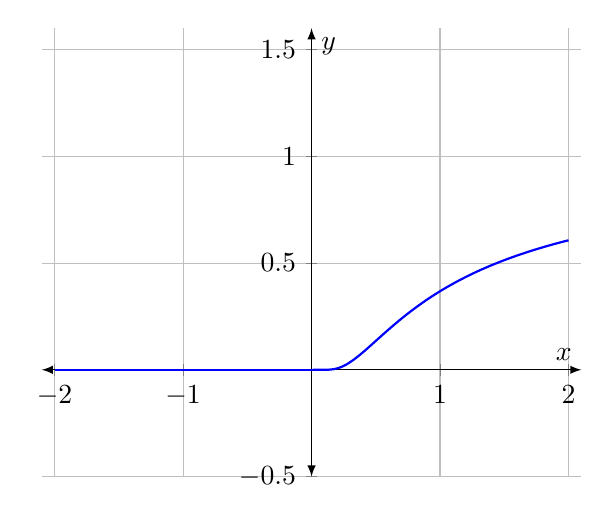
\begin{tikzpicture}
\begin{axis}[
  grid=both,
  xmin=-2.1,
  xmax=2.1,
  ymin=-0.5,
  ymax=1.6,
  axis lines=middle,
  xlabel = $x$,
  ylabel = $y$,
  axis line style={latex-latex},
  ]

\addplot[
  samples=100,
  domain=0.01:2,
  color=blue,
  thick,
  smooth,
  ]
  {(e)^(-1/x)};


\addplot[
  samples=2,
  domain=-2:0.01,
  color=blue,
  thick,
  smooth
  ]
  {0};

\end{axis}
\end{tikzpicture}

		\end{gathered}
	\]

	Comenzaremos mostrando que esta función es suave, procederemos en dos pasos:

	\begin{enumerate}
		\item La función es continua. Esto se tiene trivialmente calculando los límites laterales del cociente de Newton:
		      \begin{align*}
			      \lim_{t \to 0^+} \frac{f(t) - f(0)}{t} & = \lim_{t \to 0^+} \frac{e^{-\frac{1}{t}}}{t} = 0 \\
			      \lim_{t \to 0^-} \frac{f(t) - f(0)}{t} & = 0
		      \end{align*}
		\item Si $t > 0$, entonces la derivada $f^{(k)}$ tiene la forma $f^{(k)}(t) = p_k(t)\frac{e^{-\frac{1}{t}}}{t^{2k}}$ para algún polinomio $p_k$ con grado a lo más $k$.

		      Para $k = 0$ esto se cumplirá por definición de $f$. Supongamos que la propiedad se cumple para algún $k \geq 0$. Mostraremos que se cumple también para $f^{(k+1)}$:
		      \begin{align*}
			      f^{(k+1)}(t) & = \frac{d}{dt} f^{(k)}(t) = \frac{d}{dt} p_k(t) \frac{e^{-\frac{1}{t}}}{t^{2k}}                                                          \\
			                   & = p'_k(t) \frac{e^{-\frac{1}{t}}}{t^{2k}} + p_k(t) \frac{t^{-2} e^{-\frac{1}{t}}}{t^{2k}} - 2kp_k(t) \frac{e^{-\frac{1}{t}}}{t^{2(k+1)}} \\
			                   & = \left(t^2p'_k(t) + p_k(t) - 2ktp_k(t) \right) \frac{e^{-\frac{1}{t}}}{t^{2(k+1)}}
		      \end{align*}

		\item Claramente cuando tomamos los límite $\lim_{t \to 0^+} f^{(k)}(t)$ y $\lim_{t \to 0^-} f^{(k)}(t)$ ambos son cero.
	\end{enumerate}

	Por lo tanto $f$ es una función suave en todo $\R$

	Ahora, lo que queremos es utilizar la función $f$ para definir una función indicadora suave, el primer paso para poder lograr esto es definir la función $g: \R \to \R$ del siguiente modo:
	\[
		g(t) = \frac{f(t)}{f(t)+f(1-t)}
		\qquad \qquad
		\begin{gathered}
			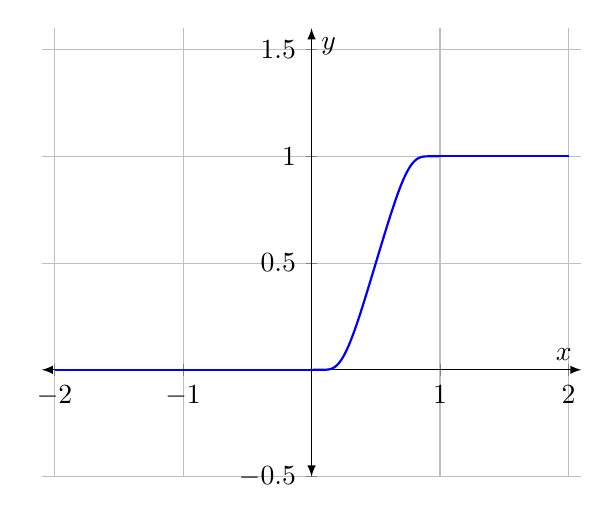
\begin{tikzpicture}
\begin{axis}[
  grid=both,
  xmin=-2.1,
  xmax=2.1,
  ymin=-0.5,
  ymax=1.6,
  axis lines=middle,
  xlabel = $x$,
  ylabel = $y$,
  axis line style={latex-latex},
  ]

\addplot[
  samples=100,
  domain=0.01:0.99,
  color=blue,
  thick,
  smooth,
  ]
  {((e)^(-1/x)) / ( ( e^(-1/x) ) + (e^(-1/(1-x))) )};


\addplot[
  samples=2,
  domain=-2:0.01,
  color=blue,
  thick,
  smooth
  ]
  {0};

\addplot[
  samples=2,
  domain=0.99:2,
  color=blue,
  thick,
  smooth
  ]
  {1};
\end{axis}
\end{tikzpicture}

		\end{gathered}
	\]


	Al ser $g$ el cociente de dos funciones suaves, y dado que el denominador no se anula en ningún punto, $g$ estará bien definida en todo $\R$ y además será suave. Lo que esta función $g$ nos da es una transición suave del $0$ al $1$, por lo cual, será sencillo construir una función indicadora suave a partir de esta, esto se logrará aplicando transformaciones sencillas.

	Si tomamos $a,b \in \R$ tales que $a<b$, podemos hacer un cambio de variables del conjunto compacto $[a^2,b^2]$ al conjunto $[0,1]$ del siguiente modo:

	\[
		x \mapsto \frac{x - a^2}{b^2 - a^2}
	\]

	Esta transformación nos permite cambiar la escala de $g$  y trasladarla en el eje horizontal,es por esta razón que se define $h: \R \to \R$ del siguiente modo,
	\[
		h(x) = g\left(\frac{x - a^2}{b^2 - a^2}\right)
		\qquad \qquad
		\begin{gathered}
			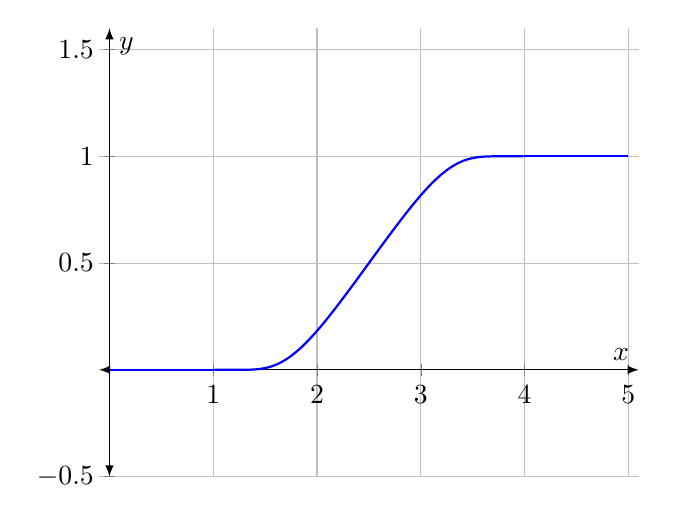
\begin{tikzpicture}
\begin{axis}[
  grid=both,
  xmin=-0.1,
  xmax=5.1,
  ymin=-0.5,
  ymax=1.6,
  axis lines=middle,
  xlabel = $x$,
  ylabel = $y$,
  axis line style={latex-latex},
  ]

\addplot[
  samples=100,
  domain=1.01:3.99,
  color=blue,
  thick,
  smooth,
  ]
  {((e)^(-1/ ((x - 1) / (4 - 1)) )) / ( ( e^(-1/ ((x - 1) / (4 - 1))) ) + (e^(-1/(1- ( (x - 1) / (4 - 1) )))) )};


\addplot[
  samples=2,
  domain=0:1.01,
  color=blue,
  thick,
  smooth
  ]
  {0};

\addplot[
  samples=2,
  domain=3.99:5,
  color=blue,
  thick,
  smooth
  ]
  {1};
\end{axis}
\end{tikzpicture}

		\end{gathered}
	\]

	Y de este modo al tomar $a,b \in \R$ como se acaba de hacer se tendrá que para $h$ se cumple lo siguiente

	\[
		h(x) = \begin{cases}
			1, & x > b^2    \\
			0, & x \leq a^2
		\end{cases}
	\]

	Ahora, podemos tomar $k(x)=h(x^2)$ para hacer que nuestra función sea simétrica alrededor del origen.

	\[
		k(x) = h(x^2) = g\left(\frac{x^2 - a^2}{b^2 - a^2}\right)
		\qquad \qquad
		\begin{gathered}
			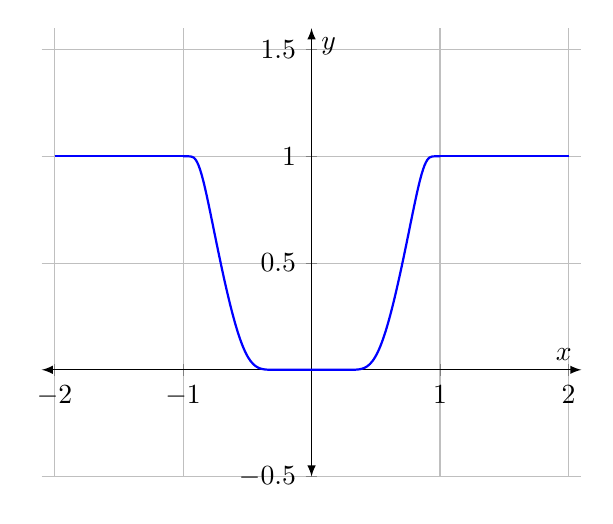
\begin{tikzpicture}
\begin{axis}[
  grid=both,
  xmin=-2.1,
  xmax=2.1,
  ymin=-0.5,
  ymax=1.6,
  axis lines=middle,
  xlabel = $x$,
  ylabel = $y$,
  axis line style={latex-latex},
  ]

\addplot[
  samples=100,
  domain=-1:1,
  color=blue,
  thick,
  smooth,
  ]
  {((e)^(-1/(x^2))) / ( ( e^(-1/(x^2)) ) + (e^(-1/(1-(x^2)))) )};


\addplot[
  samples=2,
  domain=-2:-0.99,
  color=blue,
  thick,
  smooth
  ]
  {1};

\addplot[
  samples=2,
  domain=0.99:2,
  color=blue,
  thick,
  smooth
  ]
  {1};
\end{axis}
\end{tikzpicture}

		\end{gathered}
	\]



	Y finalmente, definimos la función suave $r$ de modo que su valor sea $1$ en el intervalo y $0$ fuera de este haciendo un pequeño ajuste del siguiente modo.
	\[
		r(t) = 1 - k(x) = 1 - g\left(\frac{x^2 - a^2}{b^2 - a^2}\right)
		\qquad \qquad
		\begin{gathered}
			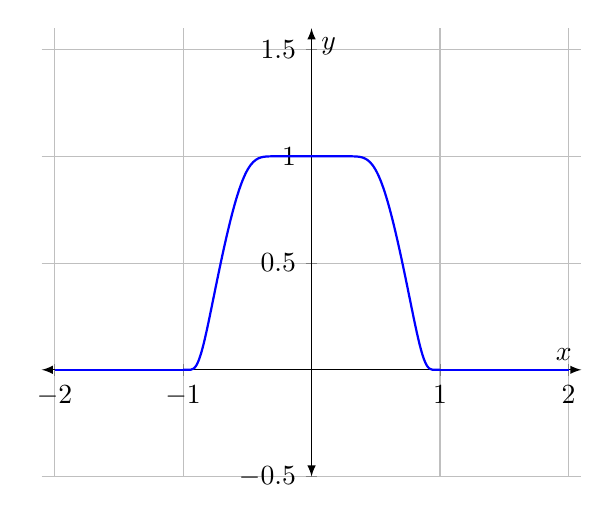
\begin{tikzpicture}
\begin{axis}[
  grid=both,
  xmin=-2.1,
  xmax=2.1,
  ymin=-0.5,
  ymax=1.6,
  axis lines=middle,
  xlabel = $x$,
  ylabel = $y$,
  axis line style={latex-latex},
  ]

\addplot[
  samples=100,
  domain=-1:1,
  color=blue,
  thick,
  smooth,
  ]
  {1 -( ((e)^(-1/(x^2))) / ( ( e^(-1/(x^2)) ) + (e^(-1/(1-(x^2)))) ))};


\addplot[
  samples=2,
  domain=-2:-0.99,
  color=blue,
  thick,
  smooth
  ]
  {0};

\addplot[
  samples=2,
  domain=0.99:2,
  color=blue,
  thick,
  smooth
  ]
  {0};
\end{axis}
\end{tikzpicture}

		\end{gathered}
	\]

	$r(t)$ es una función indicadora suave en $0$  y para cualquier $q \in \R$ tenemos que $r(x-q)$ es una función indicadora en $q$. Esta idea puede ser extendida a $\R^n$ como una función indicadora suave en $0 \in \R^n$  cuyo valor es $1$ en la bola (cerrada) $B_a(0)$ y $0$ fuera de la bola $B_b(0)$ si tomamos la función $r: \R^n \to \R$ cómo:

	\[
		\sigma(x) = r(\|x\|) = 1 - g\left(\frac{\|x\| - a^2}{b^2 - a^2}\right)
	\]
\end{example}

\begin{figure}
\centering
\begin{tikzpicture}[scale=1.25]
	\begin{axis}[
      view={30}{30},
			colormap/cool,
			xmin=-2,
			xmax=2.5,
			ymin=-2.5,
			ymax=2,
			zmin=-0.25,
			zmax=1.5,
			% axis lines=middle,
		]
		\addplot3[
			domain=-1.9:2.4,
			domain y = -2.4:1.9,
			patch,
			patch type=bilinear,
			shader=faceted interp,
		]
		{abs(x^2 + y^2) < 1 ? e^(-1 / (1 - abs(x^2 + y^2)) ) : 0 };

	\end{axis}
\end{tikzpicture}

\caption{Representación de una función indicadora suave en $\R^2$}
\end{figure}


Lo que haremos a continuación será extender estas ideas, mostraremos que para un cualquier punto en una variedad y cualquier vecindad que contenga a ese punto podemos encontrar una función indicadora suave en el punto con soporte en la vecindad.

\begin{lemma}\label{Lemma: Existencia de Función Indicadora}
	Sea $M^n$ una variedad suave, $p \in M$ un punto arbitrario y $U \subseteq M$ una vecindad de $p$. Entonces existe una función indicadora suave en $p$ con soporte en $U$.
\end{lemma}

\begin{proof}
	Sea $a$ un punto arbitrario en $M$ y $U$ una vecindad de $q$. Por ser $M$ una variedad suave existirá una carta suave $(V,\psi)$ que contiene a $q$ y tal que $V \subset U$.

	Consideremos la función $\sigma: \R^n \to \R$ definida anteriormente. $\sigma$ es una función indicadora suave en $\psi(q)$ con soporte en una bola compacta $B_r(\psi(q)) \subset V$. Definimos la función

	\[
		f(p) = \begin{cases}
			\sigma(\psi(p)), & p \in V    \\
			0,               & p \notin V
		\end{cases}
	\]

	Mostraremos que, en efecto, esta función es una función indicadora en $q$ con soporte en $U$.

	Por cómo hemos construido $\sigma$ esta tiene soporte compacto, esto es, $\sup \sigma$ es un conjunto compacto, luego $\psi^{-1}(\sup \sigma)$ será la imagen continua de un conjunto compacto, i.e., $\psi^{-1}(\sup \sigma)$ es un compacto en $M$. Dado que $M$ es Hausdorff podemos garantizar que $\psi^{-1} (\sup \sigma)$ es cerrado. Por lo tanto tendremos que
	\[
		\sup f \subset \phi^{-1} (\sup \sigma) \subset V
	\]

	Es claro que si $p \in V$, $f$ es suave en $p$ dado que $f(p)$ será la imagen de la composición de dos funciones suave. En el caso contrario, si $p \notin V$, entonces podremos elegir una carta $(W,\omega)$ que contengan a $p$ y tal que $W \cap \psi^{-1}(\sup \sigma) = \varnothing$. Entonce esta carta será también disjunta de $\sup f$, por lo que $f(W) \equiv 0$. Por lo tanto, $f$ será una función suave la cual es idénticamente $1$ en una vecindad de $V \subset U$ de $p$ y $\sup f \subset U$. Por lo tanto $f$ es una función indicadora suave en $q$ con soporte en $U$.
\end{proof}

\begin{lemma}
	Sea $M$ una variedad suave, $q$ un punto arbitrario, $U \subset M$ una vecindad de $q$ y $f$ una función indicadora suave en $q$ con soporte en $U$. Existe una función suave $\hat{f}$ en $M$ que coincide con $f$ en alguna vecindad, posiblemente más pequeña, que contiene a $q$.
\end{lemma}

\begin{proof}
	Si tomamos una función indicadora suave $r: \R^n \to \R$ cómo se construyó en el ejemplo \ref{Ex: Función Indicadora} de tal modo que $r$ tenga soporte en $U$ y esté definida en una vecindad $V$ de $q$, podemos definir la función:
	\[
		\hat{f} = \begin{cases}
			r(x)f(x), & x \in U    \\
			0,        & x \notin U
		\end{cases}
	\]

	Dado que $\hat{f}$ es el producto de funciones suaves en $U$, $\hat{f}$ es suave en $U$. Si $x \notin U$, entonces $x \notin \sup r$, por lo que existirá una vecindad que contiene a $x$ en la cual $\hat{f}$ se anula dado que, como se vio en el lema anterior, podemos tomar $\sup r$ cerrada. Por lo tanto $\hat{f}$ es suave en cada punto $x \notin U$. Y, dado que $r \equiv 1$ en $V$, la función $\hat{f}$ coincide con $f$ en $V$.
\end{proof}

Ahora utilizaremos algunos de los resultados que pueden ser encontrados en el Anexo \ref{Anexo: Topologia De Variedades} para poder dar las siguientes definiciones.

\begin{definition}[Partición de la Unidad Subordinada]\label{Definición: Partición de la Unidad Subordnada}
	Sea $M$ una variedad suave, y sea $\mathcal{U} = \{ U_\alpha \}_{\alpha \in A}$ una cubierta abierta de $M$. Una \it{partición de la unidad suave y subordinada a} $\mathcal{U}$ es una familia $\{ \phi_{\alpha} \}_{\alpha \in A}$ formada por funciones suaves y no negativas $\phi_{\alpha} : M \to \R$ tales que
	\begin{enumerate}
		\item $\sup \phi_\alpha \subseteq U_\alpha$, para cada $\alpha \in A$.
		\item La colección $\{\sup \phi_\alpha \}_{\alpha \in A}$ es localmente finita.
		\item $\sum_{\alpha \in A} \phi_\alpha (p) = 1$ para cada $p \in M$.
	\end{enumerate}
\end{definition}

Notemos que en el tercer punto de nuestra definición no tendremos problemas de convergencia dado que, por la segunda condición, al pedir que la colección de soportes de las funciones sea localmente finita, cada punto tendrá una vecindad $V$ que interceptará a $\{\sup \phi_{\alpha}\}_{\alpha \in A}$ en un subconjunto finito de $A$, por lo que la suma será finita.

\begin{theorem}[Existencia de Particiones Suave de la Unidad]\label{Teorema: Existencia de Particiones Suave de la Unidad}
	Sea $M$ una variedad suave y sea $\mathcal{U} = \{U_\alpha\}_{\alpha \in A}$ una cubierta abierta de $M$. Existe una partición suave de la unidad subordinada a $\mathcal{U}$.
\end{theorem}

\begin{proof}
	Por el resultado mostrado en el ejemplo \ref{Ex: Variedad Suave - Subvariedades Suaves}, $U_\alpha$ es en sí misma una subvariedad suave de $M$, y por los lemas \ref{Lemma: Bolas Precompactas} y \ref{Lemma: Base Por Bolas Suaves}, cada $U_\alpha$ tendrá una base $\mathcal{B}_\alpha$ formada por bolas coordinadas regulares y precompactas. Evidentemente $\mathcal{B} = \cup_{\alpha \in A} \mathcal{B}_\alpha$ formará una base para la topología de $M$.

	Por el teorema \ref{Teorema: Espacios Precompactos} y el corolario \ref{Corolario: Variedades Precompactas} podemos garantizar que $\mathcal{U}$ tendrá un refinamiento $\{B_i\}$ numerable y localmente finito que consta de elementos de $\mathcal{B}$.

	No es difícil ver que si $\{B_i\}$ es una colección localmente finita, entonces la colección formada por la cerradura de estos conjuntos $\{\overline{B}_i\}$ también será localmente finita.


	Dado que cada $B_i$ es una bola regular coordinada en algún $U_\alpha$, por definición existirá una bola coordinada suave $B_i' \subseteq U_\alpha$ tal que $\overline{B}_{i} \subseteq B_i'$, y un mapa suave $\phi_i: B_i \to \R^n$ tal que $\phi_i(\overline{B}_i) = \overline{B}_{r_i}(0)$ y $\phi_i(B_i') = B_{r_i'}(0)$ para algunos $r_i, r_i' \in \R$ tales que $r_i < r_i'$. Para cada $i$ definiremos la función $f_i: M \to R$ como:

	\[
		f_i(q)= \begin{cases}
			\rho_i \circ \phi_i, & p \in B_i'    \\
			0,                   & p \notin B_i'
		\end{cases}
	\]

	Como se mostró en el lema \ref{Lemma: Existencia de Función Indicadora} estas funciones son suaves, más aún, son funciones indicadoras suaves y además $\sup f_i = \overline{B}_i$.

	Con estas funciones podemos definir la función $f: M \to \R$ como $f(p) = \sum_i f_i(x)$. Dado que los $\{B_i\}$ y $\{\overline{B}_i\}$ son localmente finitos, la suma será finita y por lo tanto convergerá. Cómo cada $f_i$ es no negativa en cada punto en $B_i$, y cada punto de $M$ está en algún $B_i$ por ser la colección una cubierta de $M$, se sigue que $f(p) > 0$ para cada $p \in M$. Y por cómo hemos definido $\rho$ cada $f_i$ estará normalizada por lo que $0 \leq f_i \leq 1$ y $\sum_i f_i \equiv 1$.

	Por último hacemos un cambio de índices para nuestra funciones para que coincidan con los de la cubierta abierta $\mathcal{U}$. Dado que $\{B_i'\}$ es un refinamiento de $\mathcal{U}$, para cada $i$ podemos elegir algún índice $a(i) \in A$ tal que $B'_i \subseteq U_{a(i)}$. Para cada $\alpha \in A$ definimos la función $\psi_\alpha: M \to \R$ como:
	\[
		\psi_\alpha = \sum_{i : a(i) = \alpha} f_i
	\]

	Por estar cada $\psi_\alpha$ soportada en $\overline{B}_{i}$ tendremos que:
	\[
		\sup \psi_{\alpha} = \bigcup_{i: a(i)=\alpha} \subseteq U_\alpha
	\]

	Así, tendremos que la colección $\{\psi_{\alpha}\}$ es una partición de la unidad subordinada a $\mathcal{U}$.
\end{proof}

Los siguientes dos lemas nos darán maneras de extender funciones suaves utilizando particiones de la unidad, que en nuestro caso, es nuestro principal interés.

\begin{lemma}
	Sea $M$ una variedad suave, $p \in M$, $A \subset M$ un subconjunto arbitrario que contiene a $p$ y $f: A \to \R^{k}$ una función suave. Existe una extensión suave a un conjunto abierto que contiene a $A$, esto es, existe un conjunto abierto $U \subset M$ tal que $A \subset U$ y una función $\hat{f}: U \to \R^{k}$ tal que $\hat{f}|_{A \cap U} = f$.
\end{lemma}

\begin{proof}
	Consideremos una vecindad $V_p$ y una función suave $f_p: V_p \to \R^n$ para cada $p \in A$ tal que $f_{p}|_{V_p \cap A} = f|_{V_p \cap A}$. Por el teorema anterior podemos garantizar que existe una partición suave de la unidad $\{\psi_{p}\}_{p \in A}$ subordinada a $U=\cup_{p \in A}V_p$

	Definiremos el conjunto $B = \{p \in A: p \in \sup \psi_p\}$ y la función $\hat{f}: \cup_{p \in A} V_p \to \R^n$ como:
	\[
		\hat{f}(x) = \sum_{x \in B} \psi_p(x)f_p(x)
	\]

	$\hat{f}$ será una función suave que coincide con $f$ en el conjunto $U \cap A$, y por como se ha definido $U$, es claro que $A \subseteq U$.
\end{proof}

Notemos sin embargo que no siempre es posible extender una función suave a un conjunto más grande, en particular esto no siempre es posible si la función está definida en un conjunto abierto dado que el comportamiento de la función puede ser arbitrario. Como un ejemplo sencillo en $\R$ podemos tomar la función trigonométrica $\tan: (-\frac{\pi}{2}, \frac{\pi}{2}) \to \R$, para esta función no existe una extensión suave a un subconjunto abierto más grande.

Es por esto que damos el siguiente lema, el cual es un resultado más fuerte que el anterior, y nos garantiza que si imponemos la condición de que $A$ es cerrado, entonces podremos extender cualquier función suave definida en $A$ a cualquier subconjunto abierto que lo contenga a $A$.


\begin{lemma}[Lema de Extensión para Funciones Suaves]\label{Lemma: Lema de Extensión para Funciones Suaves}
	Sea $M$ una variedad suave, $A \subset M$ un subconjunto cerrado y $f: A \to \R^k$ una función suave. Para cada conjunto abierto $U$ que contiene a $A$ existe una función suave $\hat{f}: M \to \R^{k}$ tal que $\hat{f}|_{A} = f$ y $\sup(\hat{f}) = U$.
\end{lemma}

\begin{proof}
	Procederemos de modo similar a la demostración anterior. Para cada $p \in A$ tomemos una vecindad $V_p$ y una función suave $\hat{f}_p: V_p \to \R^k$ tal que $\hat{f}_p|_{V_p \cap A} = f$. Dado un conjunto abierto $U$ podemos reemplazar $V_p$ por $V_p \cap U$ y suponer que $V_p \subset U$.

	La colección de conjuntos $B=\{V_p: p \in A\} \cup (M - A)$ será una cubierta abierta para $M$, por el teorema \ref{Teorema: Existencia de Particiones Suave de la Unidad} podemos garantizar que existirá una partición suave de la unidad subordinada a la cubierta. Digamos que $\{\psi_p: p \in A\} \cup \{\psi_0 \}$ es dicha partición de tal modo que $\sup \psi_p \subseteq V_p$ y $\sup \psi_0 \subseteq M - A$.

	Definimos la función $\hat{f}: M \to \R^k$ como:
	\[
		\sum_{p \in A} \psi_p(x)\hat{f}_p(x)
	\]

	Esta suma es convergente y está formada por el producto de funciones suaves por lo que será suave, además coincide con $f$ en $U \cap A$ y tiene soporte en $U$ dado que será idénticamente cero fuera de $A$.
\end{proof}

%
% % ====================================
% % Cálculo en Variedades
% % ====================================
%
% \chapter{Título Pendiente}\label{Capítulo: Conceptos Básicos}
En este capítulo describiremos algunos conceptos básicos que eventualmente nos ayudarán a entender qué son las métricas, qué es una métrica Riemanniana y lo que son las variedades Riemannianas.

Los primeros conceptos que estudiaremos serán los espacios y fibrados tangentes. Existen varias definiciones equivalentes para lo que es un espacio tangente; nosotros procederemos a definirlo a partir de lo que llamaremos derivaciones, este enfoque tiene algunas ventajas algebraicas y se puede justificar con conceptos conocidos de cálculo multivariable. Comenzaremos contextualizando lo que queremos decir por espacio tangente en $\R^n$ y después generalizaremos la idea a variedades suaves.

Antes de comenzar necesitamos hacer la siguiente aclaración sobre la notación que utilizaremos, si consideramos un punto $p$ en $\R^n$ y queremos describir explícitamente sus coordenadas, esto lo haremos escribiendo entre paréntesis, $p = (p_1, \ldots, p_n)$; si en cambio consideramos un vector $v$ en $\R^n$, este puede ser representado por una matriz $n \times 1$, sin embargo, por conveniencia escribiremos $v = \begin{bmatrix} v_1 & \cdots & v_n \end{bmatrix}$, sin perder de vista que en realidad estamos hablando de la transpuesta de esta matriz.

\begin{definition}[Vectores y Espacios Tangentes en $\R^n$]\label{Definición: Espacio Tangente en Rn}
	Sea $a$ un punto en $\R^n$, definiremos el \it{espacio tangente a $\R^n$ en el punto $a$}, denotado por $T_a(\R^n)$, como el conjunto:
	\[ \{a\} \times \R^n = \{(a,v): v \in \R^n\} \]

	Un \it{vector tangente} a $\R^n$ es un elemento de $T_a(\R^n)$ para algún $a \in \R^n$. Denotaremos a un vector tangente $(a,v)$ particular como $v_a$ o $v|_a$ o simplemente $v$ para abreviar.
\end{definition}

En palabras más simples, lo que esta definición nos está diciendo es que el espacio tangente a $\R^n$ en algún punto $a$ es la colección de todos los vectores en $\R^n$ con origen en $a$.

Una de las propiedades más importantes del conjunto $T_a(\R^n)$ es que es un espacio vectorial bajo las operaciones

\[ v_a + w_a = (v + w)_{a}, \quad c(v)_{a} = (cv)_{a} \]

Por ser un espacio vectorial tendrá una base, no es difícil ver que si $\{e_i\}_{i=1}^n$ son los vectores de la base canónica para $\R^n$, entonces $\{e_i|_{a}\}_{i=1}^n = \{(a,e_i)\}_{i=1}^n$ será una base para $T_a(\R^n)$, al tener $n$ vectores básicos; llamamos a esta base la base estándar. $T_a(\R^n)$ será un espacio vectorial $n-$dimensional y por lo tanto será isomorfo a $\R^n$, de hecho $T_a(\R^n)$ es una copia de $\R^n$.

\begin{center}
\begin{figure}[h]
	\centering
	\begin{subfigure}{0.40\textwidth}
		\centering
    \begin{tikzpicture}
\draw[thick,->] (-0.5,0) -- (5,0) node[anchor=west]{$x$};
\draw[thick,->] (0,-0.5) -- (0,5) node[anchor=south]{$y$};

\draw (0.5,0.5) rectangle (4,4);
\node at (4.5,4.5) {$T_a(\R^n)$};

\draw[thick,->] (1,1.5) -- (3.5,1.5);
\draw[thick,->] (1.5,1) -- (1.5,3.5);
\filldraw (1.5,1.5) circle (0.1);
\node at (1,1) {$a$};
\draw[thick, ->] (1.5,1.5) -- (3,2.75);
  \node at (3.25,2.5) {$v_a$};
\end{tikzpicture}


	\end{subfigure}
	\begin{subfigure}{0.40\textwidth}
		\centering
    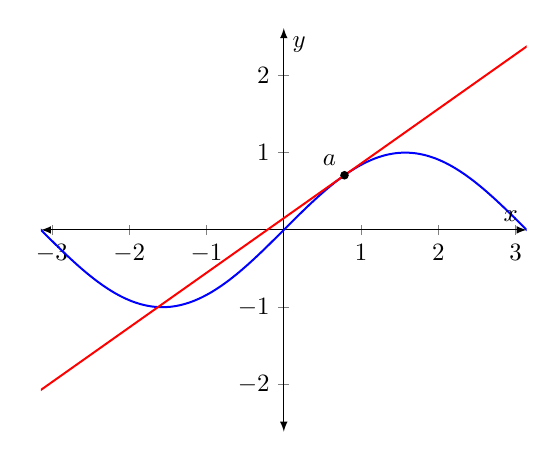
\begin{tikzpicture}[scale=0.90]
	\begin{axis}[
			% grid=both,
			xmin=-pi,
			xmax=pi,
			ymin=-1.6,
			ymax=1.6,
			axis lines=middle,
			xlabel = $x$,
			ylabel = $y$,
			axis line style={latex-latex},
      axis equal,
		]

		\addplot[
			samples=200,
			domain=-4*pi:4*pi,
			color=blue,
			thick,
			smooth,
		]
		{sin(deg(x))};

		\addplot[
			domain=-5:5,
			color=red,
      thick,
		]{( (sqrt(2) / 2) * (x - (pi/4)) ) +  (sqrt(2) / 2)};

		\addplot+[
			mark options={black},
      mark size=1.5pt,
		] coordinates {(0.785398,0.707106)} node [black, left=6pt, above=0.5pt] {$a$};
	\end{axis}
\end{tikzpicture}


	\end{subfigure}
  \\[20pt]
	\begin{subfigure}{0.40\textwidth}
		\centering
    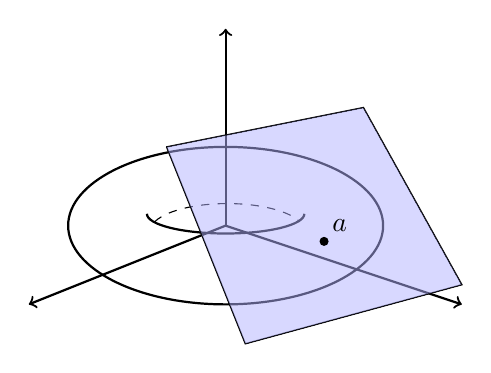
\begin{tikzpicture}

	% Ejes R3
	\draw [thick,->] (0,0) -- (0,2.5);
	\draw [thick,->] (0,0) -- (3,-1);
	\draw [thick,->] (0,0) -- (-2.5,-1);

	% Toro
	\draw [thick] (0,0) ellipse  (2 and 1);
	\draw [thick] (-1.0,0.15) arc (0:-180:-1.0 and 0.25);
  \draw [dashed] (-0.90,0.05) arc (20:160:-0.98 and 0.35);

  % Plano tangente
  \draw [line width=0.5] (-0.75,1) -- (1.75,1.5) -- (3,-0.75) -- (0.25,-1.5) -- (-0.75,1);
  \draw [fill=blue!30!white,opacity=0.5, line width=0] (-0.75,1) -- (1.75,1.5) -- (3,-0.75) -- (0.25,-1.5) -- (-0.75,1);

  % Punto $a$
	\filldraw (1.25,-0.2) circle (0.05);
	\node at (1.45,0) {$a$};
\end{tikzpicture}

	\end{subfigure}
	\begin{subfigure}{0.40\textwidth}
		\centering
    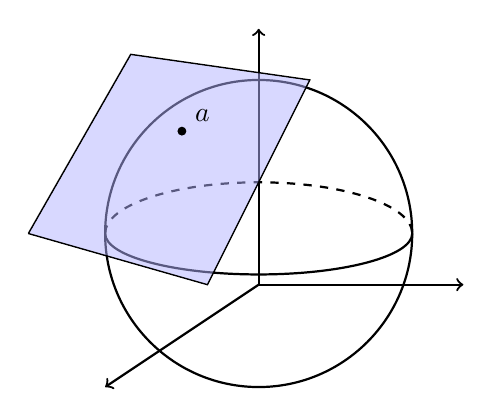
\begin{tikzpicture}[scale=0.65]
	% Esfera
	\draw [thick] (3,0) arc (0:180:3 and -0.8);
	\draw [thick, dashed] (-3,0) arc (180:0:3 and 1);
	\draw [thick] (0,0) circle (3);

	% Ejes R3
	\draw [thick,->] (0,-1) -- (0,4);
	\draw [thick,->] (0,-1) -- (4,-1);
	\draw [thick,->] (0,-1) -- (-3,-3);


	% Rectángulo (Espacio Tangente)
  \draw [fill=blue!30!white,opacity=0.5, line width=0] (-4.5,0) -- (-2.5,3.5) --(1,3.0) -- (-1,-1) -- (-4.5,0);
  \draw [line width=0.5] (-4.5,0) -- (-2.5,3.5) --(1,3.0) -- (-1,-1) -- (-4.5,0);
	\filldraw (-1.5,2) circle (0.075);
	\node at (-1.1,2.3) {$a$};
\end{tikzpicture}


	\end{subfigure}
\caption{Visualización de espacios tangentes a diferentes variedades.}
\end{figure}
\end{center}

Si en $\R^n$ consideramos un punto $a = (a_1, \dots, a_n)$ y un vector $v = \begin{bmatrix} v_1 \dots v_n \end{bmatrix}$, podemos dar la siguiente parametrización para la recta que pasa por $a$ con en la dirección de $v$:
\[ \gamma(t) = (a_1 + tv_1, \dots, a_n + tv_n) \]





\begin{definition}[Derivada Direccional]\label{Definción: Derivada Direccional}
	Sea $f: \R^n \to \R$ una función suave definida en una vecindad de un punto $a$ y $v \in T_a(\R^n)$, la \it{derivada direccional} de $f$ en $a$ en la dirección de $v$ se define como:
	\[ D_v f = \left. \frac{d}{dt} \right|_{t=0} f(\gamma(t)) \]
\end{definition}

Por la regla de la cadena podemos escribir la derivada direccional como:

\[D_v f = \sum_{i=1}^{n} \frac{d \gamma_i(0)}{dt} \frac{\partial f}{\partial x_i} (a)
	=\sum_{i=1}^n v_i \frac{\partial f}{\partial x_i} (a) \]

En este sentido, cada vector tangente $v_a \in T_a(\R^n)$ nos define un mapeo $D_v: C^{\infty}(\R^n) \to \R$ que nos da la derivada direccional de funciones suaves en un punto $a$ en la dirección de $v$. Dado que evaluamos la derivada direccional en el punto $a$, $D_v(f)$ será un número real.

Sabemos de cálculo que la derivada direccional es un operador lineal y además cumple la regla de Leibniz, esto es, si $f$ y $g$ son funciones suaves definidas en una vecindad de $a$, $c$ es una constante y $v$ es un vector tangente, entonces:

\begin{itemize}
	\item $D_v(cf) = c D_v(f)$.
	\item $D_v(f+g) = D_v(f) + D_v(g)$.
	\item $D_v(fg) = f(a) D_v(g) + g(a) D_v(f)$.
\end{itemize}

Basados en esta propiedad daremos la siguiente definición

\begin{definition}[Derivación en un punto]\label{Definición: Derivación en un punto de Rn}
	Sea $a$ un punto en $\R^n$ y $\omega: C^{\infty}(\R^n) \to \R$, diremos que $\omega$ es una \it{derivación en $a$} si es lineal y cumple la regla de Leibniz, i.e., si $f$ y $g$ son funciones suaves definidas en una vecindad de $a$, $c$ una constante

	\begin{itemize}
		\item $\omega(cf) = c \omega(f)$.
		\item $\omega(f+g) = \omega(f) + \omega(g)$.
		\item $\omega(fg) = f(a) \omega(g) + g(a) \omega(f)$.
	\end{itemize}

	Denotaremos al conjunto de todas las derivaciones de $C^{\infty}(\R^n)$ en el punto $a$ como $\D_a(\R^n)$.
\end{definition}

De modo similar a $T_a(\R^n)$, $\D_a(\R^n)$ es un espacio vectorial bajo las operaciones
\[ (\omega_1 + \omega_2)(f) = \omega_1(f) + \omega_2(f), \quad (c\omega)(f) = c(\omega(f)) \]
y más aún, con ayuda del siguiente lema probaremos que $\D_a(\R^n)$ es isomorfo a $T_a(\R^n)$.

\begin{lemma}\label{Lemma: Propiedades de las Derivaciones}
	Sea $a \in \R^n$ un punto, $\omega \in \D_a(\R^n)$ y $f,g \in C^{\infty}(\R^n)$. Entonces:
	\begin{itemize}
		\item Si $f$ es una función constante, $\omega(f) = 0$.
		\item Si $f(a) = g(a) = 0$, entonces $\omega(fg) = 0$.
	\end{itemize}
\end{lemma}

\begin{proof}
	\begin{itemize}
		\item Basta probar el caso en que $f \equiv 1$, el caso general se tiene por la linealidad de $\omega$. Si $f \equiv 1$, entonces:
		      \begin{align*}
			      \omega(f) & = \omega(f \cdot f)             \\
			                & = f(a)\omega(f) + f(a)\omega(f) \\
			                & = 2\omega(f)
		      \end{align*}
		      Esto implica que $\omega(f) = 0$.
		\item Si $f(a) = g(a) = 0$, entonces por definición de derivación se tiene que:
		      \[ \omega(fg)= f(a)\omega(g) + g(a)\omega(f) = 0  \]

	\end{itemize}
\end{proof}

Dado que las derivadas direccionales en un punto $a$ son lineales y cumplen la regla de Leibniz, estas serán derivaciones en $a$ por definición. Esto implica que existe un operador lineal $\phi$ entre $T_a(\R^n)$ y $\D_a(\R^n)$ tal que:
\begin{align*}
	\phi: T_a(\R^n) & \to \D_a(\R^n)                                                                  \\
	v               & \mapsto D_v = \left. \sum_{i=1}^{n} v_i \frac{\partial}{\partial x_i} \right|_a
\end{align*}

\begin{theorem}\label{Teorema: Isomorfismo entre Espacio Tangente y Espacio de Derivaciones}
	El mapa $\phi: T_a(\R^n) \to \D_a(\R^n)$ es un isomorfismo de espacios vectoriales.
\end{theorem}

\begin{proof}
	La linealidad se tiene trivialmente, dado que como acabamos de mencionar, las derivadas direccionales en un punto lo son. Debemos mostrar que $\phi$ es inyectiva y sobreyectiva. Para mostrar que $\phi$ es una función inyectiva, mostraremos que su kernel es cero.

	Tomemos un vector $v \in T_a(\R^n)$ tal que $D_v \equiv 0$. Si tomamos la función $f: \R^n \to \R$ como la $j-$ésima función coordenada $x_j: \R^n \to \R$ tendremos que
	\begin{align*}
		0 = D_v(x_j) & = \left. \sum_{i=1}^{n} v_i \frac{\partial}{\partial x_i} \right|_{a} x_i \\
		             & = \sum_{i=1}^{n} v_i \delta_i^j = v_j
	\end{align*}

	Dado que esto se cumple para cada $j$, se sigue que $v \equiv 0$, y por lo tanto $\phi$ es una función inyectiva.

	Para mostrar que $\phi$ es una función sobreyectiva supongamos que $\omega \in \D_a(\R^n)$, esto es, $\omega$ es una derivación en el punto $a = (a_1, \dots, a_n)$, y sea $v = \begin{bmatrix} v_1 & \cdots & v_n \end{bmatrix}$ un vector en $T_a(\R^n)$. Podemos representar a $v$ en la base estándar de $\R^n$ como $v = \sum_{i=1}^{n} v_i e_i$, si definimos a $v$ de modo que cada $v_i$ sea el número real dado por la relación $v_i = \omega(x_i)$ tendremos que $\omega = D_v$.

	En efecto, si $f: \R^n \to \R$ es una función suave definida en una vecindad de $a$, entonces, por el Teorema de Taylor tenemos que existen funciones suaves definidas en una vecindad de $a$ tal que:

	\[
		f(x) = f(a) + \sum_{i=1}^{n} \frac{\partial f}{\partial x_i} (a) (x_i - a_i) + \sum_{i=1}^{n} \sum_{j=1}^{n} (x_i - a_i)(x_j - a_j) \int_{0}^{1} (1-t) \frac{\partial^2 f}{\partial x_i \partial x_j} (a + t(x - a))
	\]

	Notemos lo siguiente, $f(a)$ es una constante y el último término es la suma del producto de dos funciones suaves, $(x_i - a_i)$ y $(x_j - a_j)$ por la integral; ambos términos se anulan en $x = a$, por lo que, por el lema anterior, al aplicar $\omega$ a la serie de Taylor el primer y el último término se anularan, obteniendo:
	\begin{align*}
		\omega(f) & = \omega(\sum_{i=1}^{n} \frac{\partial f}{\partial x_i} (a )(x_i - a_i))         \\
		          & = \sum_{i=1}^{n} \frac{\partial f}{\partial x_i} (a)(\omega(x_i) - \omega(a_i)) \\
		          & = \sum_{i=1}^{n} \frac{\partial f}{\partial x_i}(a) v_i = D_v f
	\end{align*}

	Por lo tanto $\phi$ es una función lineal, inyectiva y sobreyectiva entre espacios vectoriales, esto es, $\phi$ es un isomorfismo entre $T_a(\R^n)$ y $\D_a(\R^n)$.
\end{proof}

Este teorema nos permite identificar el espacio tangente en un punto con el espacio de de derivaciones en el mismo punto, lo cual denotamos por $T_a(\R^n) \simeq \D_a(\R^n)$, además, la existencia de este isomorfismo tiene como consecuencia el siguiente corolario.

\begin{corollary}\label{Corolario: Base de TpRn}
	Para cada $a \in \R^n$, las $n$ derivadas parciales
	\[
		\left. \frac{\partial }{\partial x_1} \right|_{a}, \dots, \left. \frac{\partial }{\partial x_n} \right|_{a}
	\]

	forman una base para el espacio tangente $T_a(\R^n)$.
\end{corollary}

Esta identificación nos permite escribir a los vectores de $\R^n$, $v = \begin{bmatrix} v_1 & \cdots & v_n \end{bmatrix}$ como una combinación lineal de la forma:

\[
  v = \left. \sum_{i = 1}^{n} v_i \frac{\partial}{\partial x_i} \right|_{a}
\]

% \subsection{Vectores Tangentes en Variedades}\label{Subsección: Espacios Tangentes en Variedades}
El último teorema nos da una motivación sobre cómo podríamos definir lo que es el espacio tangente en una variedad. Si bien en general no podemos visualizar a los vectores tangentes a un punto en una variedad como flechas, lo que sí podemos hacer es definir lo que es una derivación en un punto de una variedad.

\begin{definition}[Derivación En Un Punto De Una Variedad]
	Sea $M$ una variedad suave y sea $p \in M$ un punto. Diremos que un mapa $\omega: C^{\infty}(M) \to \R$ es una \it{derivación} en $p$ si es lineal y además cumple que:
	\[
		\omega(fg) = f(p)\omega(g) + g(p)\omega(f), \quad \forall f,g \in C^{\infty}(M).
	\]
	Llamaremos al conjunto de todas las derivaciones en un punto de una variedad al \it{espacio tangente} a la variedad en ese punto y lo denotamos por $T_p (M)$, de modo similar a los espacios de derivaciones en $\R^n$, el espacio tangente a una variedad es un espacio vectorial bajo las operaciones usuales. Llamaremos a los elementos de $T_p(M)$ \it{vectores tangentes a $M$ en $p$}.
\end{definition}

\begin{lemma}\label{Lemma: Propiedades De Las Derivaciones En Variedades}
	Supongamos que $M$ es una variedad suave, $p$ un punto de $M$, $\omega$ una derivación en $p$ y $f,g$ funcione suaves de $M$ a $\R$.
	\begin{itemize}
		\item Si $f$ es una función constante, entonces $\omega(f) = 0$.
		\item Si $f(p) = g(p) = 0$, entonces $\omega(fg) = 0$.
	\end{itemize}
\end{lemma}

\begin{proof}
	La demostración de este lema es idéntica a la demostración del lema \ref{Lemma: Propiedades de las Derivaciones}.
\end{proof}

Ahora estudiaremos como es que los mapas suaves afectan a los vectores tangentes. En el caso de los espacios Euclidianos cuando consideramos una función suave de $\R^m$ a $\R^n$ la matriz Jacobiana que representa a la derivada total de la función nos permite aproximar linealmente a la función en una vecindad mediante vectores tangentes. En las variedades en general no podemos hablar de mapas lineales, pero podemos extender la idea de la derivada total con un mapa lineal entre los espacios tangentes de las variedades, mapa al cual llamaremos diferencial o pushforward.

\begin{definition}[Diferencial de un Mapa Suave en un Punto]
	Si $M$ y $N$ son variedades suaves y $F: M \to N$ es un mapa suave, entonces, para cada punto $p \in M$ el mapa $F$ induce un mapa lineal entre los espacios tangentes $T_p(M)$ y $T_{F(p)}(N)$, denotado por $d_pF: T_p(M) \to T_{F(p)}(N)$, al cual llamaremos el \it{diferencial de $F$ en $p$}.

	El mapa $d_pF$ está dado del siguiente modo: Dada una derivación $\omega \in T_p(M)$, $dF_p$ será la derivación en el punto $F(p) \in N$ que actúa sobre funciones suaves de $N$ a $\R$ como:
	\[ d_pF(\omega)(f) = \omega(f \circ F). \]
\end{definition}

\begin{figure}[h]
	\centering
	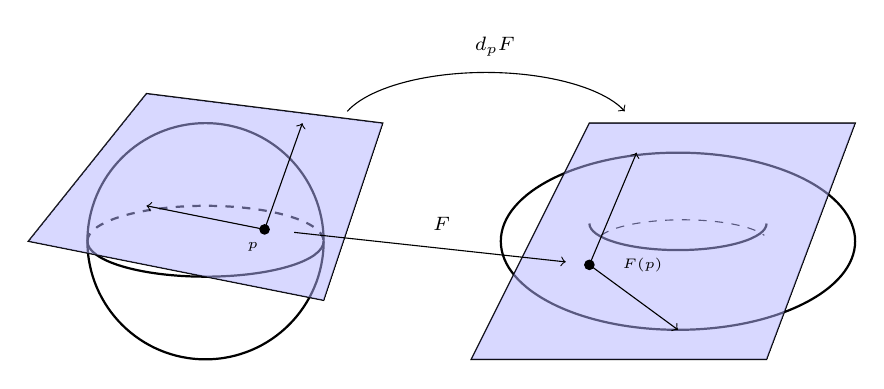
\begin{tikzpicture}[scale=1.5]
	% Esfera
	\draw [thick] (-1,0) arc (0:180:1 and -0.3);
	\draw [thick, dashed] (-3,0) arc (180:0:1 and 0.3);
	\draw [thick] (-2,0) circle (1);

	% Espacio Tangente a Esfera
	\draw [line width=0.5] (-3.5,0) -- (-2.5,1.25) -- (-0.5,1) -- (-1,-0.5) -- cycle;
	\draw [fill=blue!30!white,opacity=0.5, line width=0] (-3.5,0) -- (-2.5,1.25) -- (-0.5,1) -- (-1,-0.5) -- cycle;

	% Punto $a$
	\filldraw (-1.5,0.1) circle (0.04);
	\node at (-1.60,-0.05) {\tiny $p$};

	% Vector en $a$
	\draw [->] (-1.5,0.1) -- (-1.18,1);
	\draw [->] (-1.5,0.1) -- (-2.5,0.3);

	% Toro
	\draw [thick] (2,0) ellipse  (1.5 and 0.75);
	\draw [thick] (1.25,0.15) arc (0:-180:-0.75 and 0.225);
	\draw [dashed] (1.35,0.05) arc (20:160:-0.735 and 0.2);

	% Espacio tangente a Toro
	\draw [line width=0.5] (1.25,1) -- (3.5,1) -- (2.75,-1) -- (0.25,-1) -- cycle;
	\draw [fill=blue!30!white,opacity=0.5, line width=0] (1.25,1) -- (3.5,1) -- (2.75,-1) -- (0.25,-1) -- cycle;

	% Punto $F(a)$
	\filldraw (1.25,-0.2) circle (0.04);
	\node at (1.7,-0.2) {\tiny $F(p)$};

	% Vector en $F(a)$
	\draw[->] (1.25,-0.2) -- (1.65,0.75);
	\draw[->] (1.25,-0.2) -- (2,-0.75);

	% Lineas
	\draw[->] (-1.25,0.075) -- (1.05,-0.175);
	\node at (0,0.15) {\scriptsize $F$};


	\draw[->] (-0.8,1.1) arc (160:20:1.25 and 0.5);
	\node at (0.45,1.65) {\scriptsize $d_{p}F$};
\end{tikzpicture}

	\caption{Representación del diferencial de un mapa suave en un punto.}
\end{figure}

El diferencial $d_pF$ está bien definido dado que $F: M \to N$ y $f: N \to \R$ son funciones suaves, esto implica que $f \circ F: M \to \R$ será una función suave, por lo que $\omega(f \circ F)$ tiene sentido, la linealidad se tiene como consecuencia de que $\omega$ sea lineal y, por último, $d_pF(\omega): C^{\infty}(N) \to \R$ es una derivación en $F(p)$ dado que si $f, g \in C^{\infty}(N)$ entonces:

\begin{align*}
	d_pF(\omega)(fg) & = \omega((fg) \circ F)                                               \\
	                 & = \omega((f \circ F)(g \circ F))                                     \\
	                 & = (f \circ F)(p)\omega(g \circ F) + (g \circ F)(p) \omega(f \circ F) \\
	                 & = (f \circ F)(p)d_pF(\omega)(g) + (g \circ F)(p)d_pF(\omega)(f).
\end{align*}

A continuación, mostraremos algunas propiedades de los diferenciales de mapas suaves entre variedades, propiedades que son extensiones naturales de las propiedades conocidas de las derivadas totales del cálculo ordinario, como la linealidad del diferencial o la regla de la cadena.

\begin{lemma}\label{Lemma: Diferencial del Mapa Identidad}
	El diferencial del mapa identidad en una variedad es la identidad del espacio tangente a la variedad.
\end{lemma}

\begin{proof}
	Si $M$ es una variedad suave, $\id_M$ el mapa identidad en $M$, $p \in M$ un punto arbitrario y $\omega \in T_p(M)$ un vector tangente de $M$ en $p$, para cada $f \in C^{\infty}(M)$ se tiene:
	\begin{align*}
		d\id_{M}(\omega)(f) & = \omega(f \circ \id_M) = \omega(f).
	\end{align*}
	Dado que esto se cumple para cualquier $\omega \in T_p(M)$ y $f \in C^{\infty}(M)$, el diferencial será el mapa identidad en el espacio tangente.
\end{proof}

\begin{lemma}
	Si $M$ y $N$ son variedades suaves, $F: M \to N$ un mapa suave y $p \in M$ un punto arbitrario. El diferencial $d_pF: T_p(M) \to T_{F(p)}(M)$ es un operador lineal.
\end{lemma}

\begin{proof}
	Si $f,g \in C^{\infty}(N)$, $a \in \R$ y $\omega \in T_{p}(M)$, tenemos que:
	\begin{align*}
		d_pF(\omega)(af + g) & = \omega((af + g) \circ F)               \\
		                     & = \omega (af \circ F + g \circ F)        \\
		                     & = a\omega(f \circ F) + \omega(g \circ F) \\
		                     & = a d_pF (\omega)(f) + d_pF(\omega)(g).
	\end{align*}
	Por lo tanto, el diferencial de un mapa es un operador lineal.
\end{proof}

\begin{lemma}\label{Lemma: Regla de la Cadena para Diferenciales}
	Si $M$, $N$ y $P$ son variedades suaves, $F: M \to N$ y $G: N \to P$ mapas suaves y $p \in M$ un punto cualquiera, entonces el diferencial del mapa composición $G \circ F$ cumple la regla de la cadena, esto es,
	\[
		d_p(G \circ F) = d_{F(p)}G \circ d_pF
	\]
\end{lemma}

\begin{proof}
	Sea $\omega \in T_p(M)$ y $f \in C^{\infty}(P)$, tenemos que:
	\begin{align*}
		d_p(G \circ F) (\omega)(f) & = \omega(f \circ (G \circ F))       \\
		                           & = \omega ((f \circ G) \circ F)      \\
		                           & = d_pF(\omega)(f \circ G)           \\
		                           & = (d_{F(p)}G \circ d_pF)(\omega)(f)
	\end{align*}

	Por lo tanto, el diferencial de la composición cumple la regla de la cadena, más aún, es un mapa que lleva va del espacio tangente de $M$
	en $p$, $T_p(M)$, al espacio tangente de $P$ en $(G \circ F)(p)$, $T_{(G \circ F)(p)}(P)$.
\end{proof}

\begin{lemma}\label{Lemma: Diferencial de un Difeomorfismo}
	Si $M$ y $N$ son variedades suaves, $F: M \to N$ es un difeomorfismo y $p \in M$, entonces el diferencial $d_pF: T_p(M) \to T_{F(p)}(N)$ es un isomorfismo de espacios vectoriales y $(d_pF)^{-1} = d_{F(p)}(F^{-1})$.
\end{lemma}

\begin{proof}
	Dado que $F$ es un difeomorfismo, por definición $F$ es invertible por lo que existe una función $F^{-1}: N \to M$ tal que $F^{-1} \circ F = \id_M$ y $F \circ F^{-1} = \id_N$. Por los lemas probados anteriormente se tiene:
	\begin{align*}
		d_p(F^{-1} \circ F)      & = d_{F(p)}F^{-1} \circ d_pF = \id_{T_p(M)}       \\
		d_{F(p)}(F \circ F^{-1}) & = d_pF \circ d_{F(p)}F^{-1} = \id_{T_{F(p)}(N)}. \\
	\end{align*}
	Esto demuestra que tanto $d_pF$ como $d_{F(p)}F^{-1}$ son isomorfismos de espacios vectoriales dado que ambos son operadores lineales e invertibles, y además se comprueba que $(d_pF)^{-1} = d_{F(p)}F^{-1}$.
\end{proof}

De modo similar a la derivada total, el diferencial nos permitirá realizar cálculos en coordenadas locales, sin embargo, por cómo hemos definido al diferencial, estos operan sobre funciones definidas de manera global sobre la variedad. Al ser una generalización de la derivada total es de esperarse que puedan operar sin ambigüedad sobre subconjuntos abiertos, veremos esto a continuación.

\begin{lemma}
	Sea $M$ una variedad suave, $p \in M$ un punto arbitrario y $\omega \in T_{p}(M)$. Si $f,g \in C^{\infty}(M)$ coinciden en una vecindad de $p$, entonces $\omega(f) = \omega(g)$
\end{lemma}

\begin{proof}
	Definamos la función $h = f - g$, $h$ es una función suave que sea anula en una vecindad de $p$. Sea $\psi \in C^{\infty}(M)$ una función indicadora suave tal que $\psi(p) \equiv 1$ si $p \in \sup h$ y tal que $\sup \psi \subseteq M - \{p\}$. Dado que $\psi \equiv 1$ donde $h$ es diferente de cero, el producto $\psi h$ es idénticamente $h$. Y, como $h(p) = \psi(p) = 0$, por el lema \ref{Lemma: Propiedades De Las Derivaciones En Variedades} se tendrá que $\omega (h) = \omega (\psi h) = 0$.

	Por la linealidad de $\omega$ se sigue que $\omega(h) = \omega (f - g) = \omega(f) - \omega(g) = 0$, por lo tanto, $\omega(f) = \omega(g)$.
\end{proof}

\begin{lemma}\label{Lemma: Espacio Tangente a Subvariedad}
	Sea $M$ una variedad suave, $U \subseteq M$ un subconjunto abierto, y sea $\iota: U \to M$ el mapa de inclusión. Para cada $p \in U$, el diferencial $d_p\iota: T_p M \to T_pM$ es un isomorfismo de espacios vectoriales.
\end{lemma}

\begin{proof}
	Por el ejemplo \ref{Ex: Variedad Suave - Subvariedades Suaves} sabemos que $U$ es en sí misma una variedad suave por lo que no hay ambigüedad al considerar el espacio tangente en algún punto. La linealidad de la diferencial se tiene por definición de derivación.

	Para mostrar que el diferencial es inyectivo mostraremos que el kernel es nulo. Supongamos que $\omega \in T_{p}(U)$ y $d_p\iota(\omega) = 0 \in T_{p}(M)$. Sea $V$ una vecindad de $p$ tal que $\overline{V} \subset U$. Si $f: U \to \R$ es una función suave, por el lema \ref{Lemma: Lema de Extensión para Funciones Suaves} podemos garantizar que existe una función $\hat{f}: M \to \R$ que coincide con $f$ en $\overline{V}$. Luego, por el lema anterior se tiene que, como $f$ y $\hat{f}\big|_{U}$ son funciones suaves que coinciden en una vecindad de $p$, entonces:
	\begin{align*}
		\omega(f) & = \omega \left(\hat{f} \big|_{U} \right)\\
		          & = \omega(\hat{f} \circ \iota)   \\
		          & = d_p\iota(\omega)(\hat{f}) = 0
	\end{align*}

	Esto se cumplirá para cada función suave $f \in C^{\infty}(U)$, por lo que $\omega \equiv 0$, lo cual implica que $d\iota_p$ es inyectiva.

	Para mostrar que el diferencial del mapa de inclusión es sobreyectivo supongamos que $\omega \in T_p(M)$ es algún vector tangente arbitrario en $M$. Definamos al operador $\upsilon: C^{\infty}(U) \to \R$ de tal modo que $\upsilon(f) = \omega (\hat{f})$, donde $\hat{f}$ es cualquier función suave en $M$ que coincida con $f$ en $\overline{V}$, por el lema anterior $\upsilon(f)$ no depende de la elección de la función $\hat{f}$, por lo que $\upsilon$ está bien definida y es una derivación. Para cada función $g \in C^{\infty}(M)$ se cumple:
	\begin{align*}
		d_p\iota(\upsilon)(g)
		 & = \upsilon(g \circ \iota)                                  \\
		 & = \omega \left( (g \circ \iota) \big|_{V} \right) \\
		 & = \omega(g).
	\end{align*}
	Por lo tanto, $d\iota_p$ es un sobreyectivo, y por lo tanto será un isomorfismo entre los espacios vectoriales $T_p(U)$ y $T_p(M)$.
\end{proof}

\begin{theorem}[Invariancia de la Dimensión]\label{Teorema: Invariancia de la Dimensión}
	Si $M$ es una variedad suave, $n-$dimensional. Para cada $p \in M$, el espacio tangente $T_p(M)$ es un espacio vectorial $n-$dimensional.
\end{theorem}

\begin{proof}
	Para cada $p \in M$ podemos elegir una carta suave $(U, \phi)$ que contenga a $p$. Por definición $\phi$ es un difeomorfismo de $U$ a $\R^n$. El lema \ref{Lemma: Diferencial de un Difeomorfismo} nos dice que $T_{p}(U)$ y $T_{\phi(p)}(\R^n)$ son isomorfos, y el lema anterior garantiza que $T_{p}(U)$ y $T_{p}(M)$ también son isomorfos, por lo tanto, $T_{p}(M) \simeq T_{\phi(p)}(\R^n)$. De aquí que $\dim T_p(M) = \dim T_{\phi(p)}(\R^n) = n$.
\end{proof}

Una consecuencia inmediata del teorema \ref{Teorema: Isomorfismo entre Espacio Tangente y Espacio de Derivaciones} y el teorema anterior, \ref{Teorema: Invariancia de la Dimensión} es el siguiente corolario que nos da una identificación canónica de los elementos de cualquier espacio vectorial finito dimensional con los elementos de su espacio tangente, y, a su vez, dar una identificación canónica entre cada espacio tangente a un punto de una variedad y un espacio vectorial.

\begin{corollary}
	Sea $V$ un espacio vectorial finito dimensional con su estructura de variedad suave estándar. Para cada punto $a \in V$, el mapa $D_v: C^{\infty}(V) \to \R$ definido por:
	\[D_vf = \left. \frac{d}{dt} \right|_{t=0} f(a+tv), \]
	es un isomorfismo de $V$a $T_a(V)$.
\end{corollary}

% \subsection{Vectores Tangentes en Coordenadas}\label{Subsección: Espacios Tangentes en Coordenadas}
Las ideas presentadas anteriormente nos son de mucha utilidad, dado que como veremos en esta sección los espacios tangentes y los diferenciales nos permiten realizar cálculos concretos en las variedades suaves.

Sean $M$ una variedad suave $n-$dimensional, $p \in M$ algún punto y $(U,\phi)$ una carta suave que contiene a $p$. Definiremos los mapas $\phi_i: U \to \R$ como $\phi_{i} = x_i \circ \phi$, donde $x_i$ son los elementos de la base estándar de $\R^n$.

Si $f$ es un mapa suave definido en una vecindad de $p$, tomaremos:
\[
	\left.
	\frac{\partial}{\partial \phi_i}
	\right|_{p} f
	=
	\left.
	\frac{\partial}{\partial x_i}
	\right|_{\phi(p)}
	\left( f \circ \phi^{-1} \right).
\]
Evidentemente cada $\frac{\partial}{\partial \phi_i}$ es una derivación, por lo que serán vectores tangentes en $T_p(M)$, y por definición $\phi: U \to \R^n$ es un difeomorfismo. Sabiendo esto y por el lema \ref{Lemma: Diferencial de un Difeomorfismo} podemos garantizar que el diferencial $d_p\phi: T_p(M) \to T_{\phi(p)}(\R^n)$ es un isomorfismo de espacios vectoriales.

\begin{lemma}\label{Lemma: Definicion Vector Coordenado}
	Sean $M$ una variedad suave, $p \in M$ un punto arbitrario y $(U,\phi) = (U, \phi_1, \dots, \phi_n)$ una carta suave que contiene a $p$, entonces:
	\[
		d_p\phi \left( \left. \frac{\partial }{\partial \phi_i}\right|_{p}\right)
    = \left. \frac{\partial}{\partial x_i} \right|_{\phi(p)}.
	\]
\end{lemma}

\begin{proof}
	Sea $f: \R^n \to \R$ cualquier función suave definida en una vecindad de $\phi(p)$, se tendrá que:
	\begin{align*}
		d_p\phi \left( \left. \frac{\partial}{\partial \phi_i} \right|_{p} \right) f
		 & = \left. \frac{\partial}{\partial \phi_i} \right|_{p}
		f \circ \phi                                                  \\
		 & = \left. \frac{\partial}{\partial x_i} \right|_{\phi(p)}
		f \circ \phi \circ \phi^{-1}                                  \\
		 & = \left. \frac{\partial}{\partial x_i}\right|_{\phi(p)} f.
	\end{align*}
\end{proof}

\begin{theorem}\label{Teorema: Base para el espacio tangente}
	Sean $M$ una variedad suave, $p \in M$ y $(U,\phi) = (U, \phi_1, \dots, \phi_n)$ una carta suave que contiene a $p$. El espacio tangente $T_p(M)$ tiene como base a la colección:
	\[
		\left. \frac{\partial}{\partial \phi_1} \right|_p, \hdots, \left. \frac{\partial}{\partial \phi_n} \right|_p .
	\]
\end{theorem}

\begin{proof}
	El corolario \ref{Corolario: Base de TpRn} nos dice que las derivadas parciales forman una base para $T_p(\R^n)$, además el lema anterior nos dice que el mapa:
	\begin{align*}
		d_p\phi: T_p(M)                                     & \to \T_{\phi(p)} (\R^n) \\
		\left. \frac{\partial}{\partial \phi_i} \right|_{p} & \mapsto
		\left. \frac{\partial}{\partial x_i} \right|_{\phi(p)},
	\end{align*}

	es un isomorfismo, y como los isomorfismos llevan bases de un espacio vectorial a bases de otros espacios vectoriales tendremos que el conjunto $\left\{ \frac{\partial}{\partial \phi_{i}}|_{p} \right\}_{i=1}^{n}$ es una base para $T_{p}(M)$.
\end{proof}

Como hemos mencionado, el diferencial de un mapa suave entre variedades ha sido de tal modo que este sea una generalización de la derivada total conocida del cálculo en $\R^n$, la cual puede ser representada por la matriz Jacobiana, sin embargo, una ventaja que tenemos con el diferencial es que es independiente de las coordenadas que se elijan, esto es, no depende de las bases que se pudiesen elegir para los espacios tangentes a las variedades. Aun así, es posible dar una representación matricial para el diferencial, evidentemente esta representación sí dependerá de las coordenadas elegidas.

Comenzaremos viendo que, en efecto, la representación matricial coincidirá con lo que se podría esperar en espacios euclidianos, esto es, que la matriz sea la matriz Jacobiana.

Consideremos dos espacios euclidianos $\R^n$ y $\R^m$, donde $\{x_1, \dots, x_n\}$ y $\{y_1, \dots, y_m\}$ son las bases estándar respectivas de cada espacio. Sean $U \subseteq \R^n$ y $V \subseteq \R^m$ subconjuntos abiertos, $p \in U$ un punto arbitrario y $F: U \to V$ una función suave. Utilizando la regla de la cadena para calcular el diferencial de $F$ en $p$ tenemos:
\begin{align*}
	d_{p}F
	\left(
	\left. \frac{\partial}{\partial x_i} \right|_{p}
	\right)
	 & =
	\left. \frac{\partial}{\partial x_i} \right|_{p} (f \circ F) \\
	 & =
	\sum_{j=1}^{n} \frac{\partial f}{\partial y_j} F(p)
	\frac{\partial F_j}{\partial x_i} (p)                        \\
	 & =
	\sum_{j=1}^{n}
	\left(
	\frac{\partial F_j}{\partial x_i} (p)
	\left.
	\frac{\partial}{\partial y_j}
	\right|_{F(p)}
	\right) f.                                                   \\
	\implies d_p F
	\left(
	\left. \frac{\partial}{\partial x_i} \right|_p
	\right)
	 & =
	\sum_{j=1}^{n}
	\frac{\partial F_j}{\partial x_i} (p)
	\left.
	\frac{\partial}{\partial y_j}
	\right|_{F(p)}.
\end{align*}
Por lo tanto, la representación matricial de $d_{p}F$ en términos de las bases elegidas para $\R^n$ y $\R^m$ es:

\[
	\begin{bmatrix}
		\frac{\partial F_1}{\partial x_1}(p) & \hdots & \frac{\partial F_1}{\partial x_n}(p) \\[24pt]
		\vdots                               & \ddots & \vdots                               \\[24pt]
		\frac{\partial F_m}{\partial x_1}(p) & \hdots & \frac{\partial F_m}{\partial x_n}(p)
	\end{bmatrix}.
\]

Esto es precisamente lo que cabría esperarse, que la representación en coordenadas del diferencial de una función suave sea precisamente la matriz Jacobiana, por lo que coincide con la derivada total.

Para ver qué sucede con el caso general consideremos dos variedades suaves $M$ y $N$, un punto $p \in M$ y un mapa suave $F: M \to N$. Tomemos dos cartas $(U,\phi)$ y $(V,\psi)$ que contengan a $p$ y $F(p)$ respectivamente.
\begin{figure}[h]
  \center
	\tikzexternaldisable % Desactiva el precompilado de figuras, ¡No quitar!
\begin{tikzcd}
	M \arrow[d, "\varphi"'] \arrow[r, "F"] & N \arrow[d, "\psi"] \\
	\mathbb{R}^m \arrow[r, "\hat{F}"']     & \mathbb{R}^n
\end{tikzcd}
\tikzexternalenable % Restaura la el precompilado de figuras.

	\caption*{Diagrama de la representación coordenada de un mapa.}
\end{figure}
Como se vio en la sección \ref{Sección: Mapas Suaves} el mapa $F$ tiene una representación en coordenadas dada por $\hat{F} = \psi \circ F \circ \phi^{-1}: \phi(U \cap F^{-1}(V)) \to \psi(V)$. Por los cálculos anterior podemos representar el diferencial de $\hat{F}$ en $\phi(p)$ con respecto a la base estándar por la matriz Jacobiana de $\hat{F}$ en $\phi(p)$. Utilizando el hecho de que $F \circ \phi^{-1} = \psi^{-1} \circ \hat{F}$, calculando obtenemos:
\begin{align*}
	d_{p}F \left( \left. \frac{\partial}{\partial \phi_i} \right|_{p}\right) & =
	d_p(\psi^{-1}\circ\hat{F}\circ \phi)\left(\left.\frac{\partial}{\partial \phi_i}\right |_p\right) \\
	                                                                         & =
	\left. d_p \psi^{-1} \right|_{\hat{F}(\phi(p))}
	\Biggl(
	d_{\phi(p)} \hat{F}
	\Biggl(
	\underbrace{d_p \phi
		\left(
		\left. \frac{\partial}{\partial \phi_i} \right|_{p}
		\right)}_{\left. \frac{\partial}{\partial x_i} \right|_{\phi (p)}}
	\Biggr)	\Biggr)                                                                                   \\
	                                                                         & =
	\left. d_p \psi^{-1} \right|_{\hat{F}(\phi(p))}
	\left(
	\sum_{j=1}^{n} \frac{\partial \hat{F_j}}{\partial x_i} \left( \phi(p) \right)
	\left. \frac{\partial}{\partial y_j} \right|_{F(\phi(p))}
	\right)                                                                                           \\
	                                                                         & =
	\sum_{j=1}^{n} \frac{\partial \hat{F}_j}{\partial x_i} (\phi(p))
	\left. d_p \psi^{-1} \right|_{\hat{F}(\phi(p))}
	\left(
	\left. \frac{\partial}{\partial y_j}\right|_{F(\phi(p))}
	\right)                                                                                           \\
	                                                                         & =
	\sum_{j=1}^{n} \frac{\partial \hat{F}_j}{\partial x_i} (\phi(p))
	\left.
	\frac{\partial}{\partial \psi_{j}}
	\right|_{\hat{F}(\phi(p))}.
\end{align*}

Por lo tanto, podemos representar el diferencial $dF_p$ con la matriz Jacobiana de la representación coordenada del mapa $F$.

Como estas representaciones dependen de la base elegida será necesario tener una manera en la que podamos transformar de unas coordenadas a otras. Consideremos una variedad suave $M$, dos cartas suaves $(U,\phi)=(U,\phi_1,\dots,\phi_n)$ y $(V,\psi)=(V,\psi_1,\dots,\psi_n)$, y un punto $p \in M$ que también pertenezca a la intersección $p \in U \cap V$. Los vectores tangentes en $p$ pueden ser representados respecto a las bases $\left\{\left. \frac{\partial}{\partial \phi_i} \right|_{p}\right\}_{i=1}^{n}$ y $\left\{\left. \frac{\partial}{\partial \psi_i} \right|_{p}\right\}_{i=1}^{n}$.

Naturalmente la representación de cualquier vector tangente está relacionada con cualquier otra representación, a continuación, veremos cómo es que las representaciones están relacionadas. Tomemos el diferencial del mapa de transición $\psi \circ \phi^{-1}: \phi(U \cap V) \to \R^n$.

\[
	d_{\phi(p)}(\psi \circ \phi^{-1}) \left( \left. \frac{\partial}{\partial \phi_{i}} \right|_{\phi(p)} \right) = \sum_{j=1}^{n}\frac{\partial \psi_j}{\partial \phi_i} (\phi(p)) \left. \frac{\partial}{\partial \psi_{j}} \right|_{\psi(p)}.
\]

Una consecuencia inmediata del lema \ref{Lemma: Definicion Vector Coordenado} es la siguiente representación de los vectores tangentes, de la cual, junto con la identidad anterior se seguirá la cadena de igualdades:

\begin{align*}
	\left. \frac{\partial}{\partial \phi_i}\right|_{p}
	 & =
	d_{\phi(p)} \left(\phi^{-1}\right)
	\left(\left.
	\frac{\partial}{\partial \phi_i}
	\right|_{\phi(p)}\right)                                            \\
	 & =
	d_{\psi(p)}(\psi^{-1}) \circ d_{\phi(p)}\left(\psi \circ \phi^{-1}\right)
	\left( \left.
	\frac{\partial}{\partial \phi_i}
	\right|_{\phi(p)}\right)                                            \\
	 & =
	d_{\psi(p)}(\psi^{-1}) \left(
	\sum_{j=1}^{n}\frac{\partial \psi_j}{\partial \phi_i}(\phi(p))
	\left.
	\frac{\partial}{\partial \psi_j}
	\right|_{\psi(p)} \right)                                           \\
	 & = \sum_{j=1}^{n}\frac{\partial \psi_j}{\partial \phi_i}(\phi(p))
	\left.
	\frac{\partial}{\partial \psi_j}
	\right|_{p}.
\end{align*}

Por lo tanto, si tenemos un vector tangente $\omega \in T_p(M)$ con dos representaciones diferentes, digamos:
\[
	\omega = \sum_{i=1}^{n} v_i \frac{\partial}{\partial \phi_i}
	\quad \text{y} \quad
	\omega = \sum_{j=1}^{n} w_j \frac{\partial}{\partial \psi_j}.
\]
Donde $v_i$ y $w_i$ son constantes que dependen de $\omega$, y podemos transformar las constantes del siguiente modo:
\[
	w_j = \sum_{i=1}^{n} \frac{\partial \psi_j}{\partial \phi_i} (\phi(p)) v_i.
\]

\begin{example}
	Consideremos el mapa de transición entre las coordenadas esféricas y las coordenadas estándar en subconjuntos abiertos adecuados de $\R^{3}$, el cual está por la igualdad $(x,y,z) = (r \cos \phi \sin \theta, r \sin \phi \sin \theta, r\cos \theta)$. Tomemos el punto $p \in \R^{3}$ con representación en coordenadas esféricas $p = (r,\theta,\phi) = (2,\frac{\pi}{4},\frac{\pi}{4})$ y tomemos un vector tangente $\omega \in T_p(\R^3)$ cuya representación en coordenadas polares esté dada por:
	\[
		\omega = \left. \frac{\partial}{\partial r} \right|_p -
		\left. 2\frac{\partial}{\partial \theta} \right|_p +
		\left. 3\frac{\partial}{\partial \phi} \right|_p.
	\]
	Si queremos transformar este vector tangente a coordenadas estándar necesitaremos utilizar la fórmula que acabamos de deducir de cambio de coordenadas. Calculando las constantes $v_i$:
	\begin{align*}
		v_1 & =
		\left. \frac{\partial}{\partial r} r\cos(\phi)\sin(\theta) \right|_p
		\frac{\partial}{\partial x} +
		\left. \frac{\partial}{\partial r} r\sin(\phi)\sin(\theta)\right|_p
		\frac{\partial}{\partial y} +
		\left. \frac{\partial}{\partial r}r\cos(\theta)\right|_{p}
		\frac{\partial}{\partial z}                                          \\
		    & = \cos(\phi)\sin(\theta)|_p \frac{\partial}{\partial x}
		+ \sin(\phi)\sin(\theta)|_p  \frac{\partial}{\partial y}
		+ \cos(\theta)|_p \frac{\partial}{\partial z}                        \\
		    & = \frac{1}{2} \frac{\partial}{\partial x}
		+ \frac{1}{2} \frac{\partial}{\partial y}
		+ \frac{\sqrt{2}}{2} \frac{\partial}{\partial z}.                    \\
		v_2 & =
		\left. \frac{\partial}{\partial \theta} r\cos(\phi)\sin(\theta) \right|_p
		\frac{\partial}{\partial x} +
		\left. \frac{\partial}{\partial \theta} r\sin(\phi)\sin(\theta)\right|_p
		\frac{\partial}{\partial y} +
		\left. \frac{\partial}{\partial \theta}r\cos(\theta)\right|_{p}
		\frac{\partial}{\partial z}                                          \\
		    & = r\cos(\phi)\cos(\theta)|_p \frac{\partial}{\partial x}
		+ r\sin(\phi)\cos(\theta)|_p  \frac{\partial}{\partial y}
		- r\sin(\theta)|_p \frac{\partial}{\partial z}                       \\
		    & = \frac{\partial}{\partial x} + \frac{\partial }{\partial y}
		- \frac{\partial}{\partial z}.                                       \\
		v_3 & =
		\left. \frac{\partial}{\partial \phi} r\cos(\phi)\sin(\theta) \right|_p
		\frac{\partial}{\partial x} +
		\left. \frac{\partial}{\partial \phi} r\sin(\phi)\sin(\theta)\right|_p
		\frac{\partial}{\partial y} +
		\left. \frac{\partial}{\partial \phi} r\cos(\theta)\right|_{p}
		\frac{\partial}{\partial z}                                          \\
		    & = -r\sin(\phi)\sin(\theta)|_p \frac{\partial}{\partial x}
		+ r\cos(\phi)\sin(\theta)|_p  \frac{\partial}{\partial y}            \\
		    & = - \frac{\partial}{\partial x} + \frac{\partial}{\partial y}.
	\end{align*}
	Por lo tanto, podemos sustituir en la ecuación que nos da el vector tangente para obtener su representación en coordenadas estándar, obteniendo:
	\[ \omega =
		\left. -\frac{9}{2} \frac{\partial}{\partial x} \right|_p +
		\left. \frac{3}{2}\frac{\partial}{\partial y} \right|_p +
		\left. \frac{\sqrt{2} - 4}{2} \frac{\partial}{\partial z} \right|_p .\]
\end{example}

% \subsection{El Fibrado Tangente}\label{Subsección: Fibrado Tangente}
Por la definición que hemos dado de espacio tangente, estos están definidos en cada punto de una variedad suave, sin embargo, para algunos fines es más conveniente considerar todos los espacios tangentes a una variedad de forma simultánea. Es con este propósito que definiremos al Fibrado Tangente de una variedad suave, este objeto nos dará una manera de organizar los espacios tangentes de una variedad suave de tal modo que el objeto resultante sea en sí mismo una variedad suave.

\begin{center}
	\begin{figure}[h!]
		\centering
		\begin{subfigure}{0.35\textwidth}
			\centering
			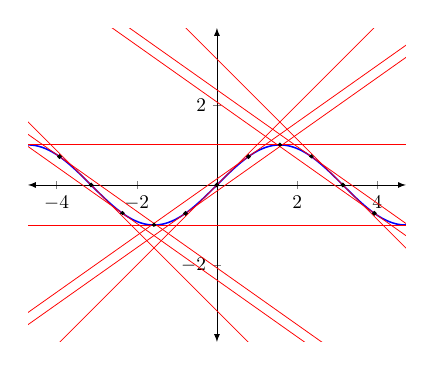
\begin{tikzpicture}[scale=0.70]
	\begin{axis}[
			% grid=both,
			xmin=-3*pi/2,
			xmax=3*pi/2,
			ymin=-1.6,
			ymax=1.6,
			axis lines=middle,
			axis line style={latex-latex},
			axis equal,
		]

		\addplot[
			samples=200,
			domain=-4*pi:4*pi,
			color=blue,
			thick,
			smooth,
		]
		{sin(deg(x))};
\addplot[domain=-5:5,color=red,thin]{-0.707107 * (x + 3.926991) + 0.707107};
\addplot+[mark=*, mark options={black},mark size=1pt] coordinates {( -3.926991 , 0.707107 )};
\addplot[domain=-5:5,color=red,thin]{-1.000000 * (x + 3.141593) + -0.000000};
\addplot+[mark=*, mark options={black},mark size=1pt] coordinates {( -3.141593 , -0.000000 )};
\addplot[domain=-5:5,color=red,thin]{-0.707107 * (x + 2.356194) + -0.707107};
\addplot+[mark=*, mark options={black},mark size=1pt] coordinates {( -2.356194 , -0.707107 )};
\addplot[domain=-5:5,color=red,thin]{0.000000 * (x + 1.570796) + -1.000000};
\addplot+[mark=*, mark options={black},mark size=1pt] coordinates {( -1.570796 , -1.000000 )};
\addplot[domain=-5:5,color=red,thin]{0.707107 * (x + 0.785398) + -0.707107};
\addplot+[mark=*, mark options={black},mark size=1pt] coordinates {( -0.785398 , -0.707107 )};
\addplot[domain=-5:5,color=red,thin]{1.000000 * (x - 0.000000) - -0.000000};
\addplot+[mark=*, mark options={black},mark size=1pt] coordinates {( 0.000000 , 0.000000 )};
\addplot[domain=-5:5,color=red,thin]{0.707107 * (x - 0.785398) - -0.707107};
\addplot+[mark=*, mark options={black},mark size=1pt] coordinates {( 0.785398 , 0.707107 )};
\addplot[domain=-5:5,color=red,thin]{-0.000000 * (x - 1.570796) - -1.000000};
\addplot+[mark=*, mark options={black},mark size=1pt] coordinates {( 1.570796 , 1.000000 )};
\addplot[domain=-5:5,color=red,thin]{-0.707107 * (x - 2.356195) - -0.707107};
\addplot+[mark=*, mark options={black},mark size=1pt] coordinates {( 2.356195 , 0.707107 )};
\addplot[domain=-5:5,color=red,thin]{-1.000000 * (x - 3.141593) - 0.000000};
\addplot+[mark=*, mark options={black},mark size=1pt] coordinates {( 3.141593 , -0.000000 )};
\addplot[domain=-5:5,color=red,thin]{-0.707107 * (x - 3.926991) - 0.707107};
\addplot+[mark=*, mark options={black},mark size=1pt] coordinates {( 3.926991 , -0.707107 )};	\end{axis}
\end{tikzpicture}

		\end{subfigure}
		\hspace{40pt}
		\begin{subfigure}{0.35\textwidth}
			\centering
			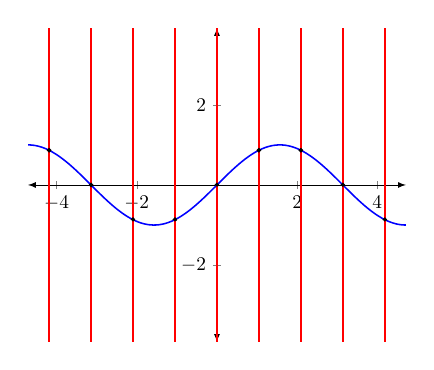
\begin{tikzpicture}[scale=0.70]
	\begin{axis}[
			% grid=both,
			xmin=-3*pi/2,
			xmax=3*pi/2,
			ymin=-1.6,
			ymax=1.6,
			axis lines=middle,
			axis line style={latex-latex},
			axis equal,
		]

		\addplot[
			samples=200,
			domain=-4*pi:4*pi,
			color=blue,
			thick,
			smooth,
		]
		{sin(deg(x))};

\addplot+[mark=*, mark options={black},mark size=1pt] coordinates {( -4.188790 , 0.866025 )};
\addplot[thick, smooth,domain=-pi:pi,red] coordinates {(-4.188790,-5)(-4.188790,5)};
\addplot+[mark=*, mark options={black},mark size=1pt] coordinates {( -3.141593 , -0.000000 )};
\addplot[thick, smooth,domain=-pi:pi,red] coordinates {(-3.141593,-5)(-3.141593,5)};
\addplot+[mark=*, mark options={black},mark size=1pt] coordinates {( -2.094395 , -0.866025 )};
\addplot[thick, smooth,domain=-pi:pi,red] coordinates {(-2.094395,-5)(-2.094395,5)};
\addplot+[mark=*, mark options={black},mark size=1pt] coordinates {( -1.047197 , -0.866025 )};
\addplot[thick, smooth,domain=-pi:pi,red] coordinates {(-1.047197,-5)(-1.047197,5)};
\addplot+[mark=*, mark options={black},mark size=1pt] coordinates {( 0.000000 , 0.000000 )};
\addplot[thick, smooth,domain=-pi:pi,red] coordinates {(0.000000,-5)(0.000000,5)};
\addplot+[mark=*, mark options={black},mark size=1pt] coordinates {( 1.047198 , 0.866025 )};
\addplot[thick, smooth,domain=-pi:pi,red] coordinates {(1.047198,-5)(1.047198,5)};
\addplot+[mark=*, mark options={black},mark size=1pt] coordinates {( 2.094395 , 0.866025 )};
\addplot[thick, smooth,domain=-pi:pi,red] coordinates {(2.094395,-5)(2.094395,5)};
\addplot+[mark=*, mark options={black},mark size=1pt] coordinates {( 3.141593 , -0.000000 )};
\addplot[thick, smooth,domain=-pi:pi,red] coordinates {(3.141593,-5)(3.141593,5)};
\addplot+[mark=*, mark options={black},mark size=1pt] coordinates {( 4.188790 , -0.866026 )};
\addplot[thick, smooth,domain=-pi:pi,red] coordinates {(4.188790,-5)(4.188790,5)};	

\end{axis}
\end{tikzpicture}

		\end{subfigure}
		\\[20pt]
		\begin{subfigure}{0.35\textwidth}
			\centering
			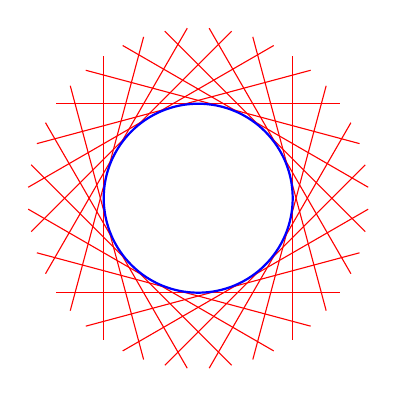
\begin{tikzpicture}[scale=1.20]
  % Lineas iniciales
  \draw[red] (-1,-1.5) -- (-1,1.5);
  \draw[red] (1,-1.5)  -- (1,1.5);
  \draw[red] (-1.5,1)  -- (1.5,1);
	\draw[red] (-1.5,-1) -- (1.5,-1);

	\begin{scope}[rotate around={15:(0,0)}]
		\draw[red] (-1,-1.5) -- (-1,1.5);
		\draw[red] (1,-1.5)  -- (1,1.5);
		\draw[red] (-1.5,1)  -- (1.5,1);
		\draw[red] (-1.5,-1) -- (1.5,-1);
	\end{scope}
	\begin{scope}[rotate around={30:(0,0)}]
		\draw[red] (-1,-1.5) -- (-1,1.5);
		\draw[red] (1,-1.5)  -- (1,1.5);
		\draw[red] (-1.5,1)  -- (1.5,1);
		\draw[red] (-1.5,-1) -- (1.5,-1);
	\end{scope}
	\begin{scope}[rotate around={45:(0,0)}]
		\draw[red] (-1,-1.5) -- (-1,1.5);
		\draw[red] (1,-1.5)  -- (1,1.5);
		\draw[red] (-1.5,1)  -- (1.5,1);
		\draw[red] (-1.5,-1) -- (1.5,-1);
	\end{scope}
	\begin{scope}[rotate around={60:(0,0)}]
		\draw[red] (-1,-1.5) -- (-1,1.5);
		\draw[red] (1,-1.5)  -- (1,1.5);
		\draw[red] (-1.5,1)  -- (1.5,1);
		\draw[red] (-1.5,-1) -- (1.5,-1);
	\end{scope}
	\begin{scope}[rotate around={75:(0,0)}]
		\draw[red] (-1,-1.5) -- (-1,1.5);
		\draw[red] (1,-1.5)  -- (1,1.5);
		\draw[red] (-1.5,1)  -- (1.5,1);
		\draw[red] (-1.5,-1) -- (1.5,-1);
	\end{scope}

	\draw[blue,thick] (0,0) circle (1);
\end{tikzpicture}

		\end{subfigure}
		\hspace{30pt}
		\begin{subfigure}{0.35\textwidth}
			\centering
			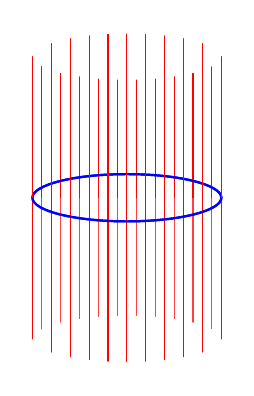
\begin{tikzpicture}[scale=1.20]
  \path[use as bounding box] (-1.05,-1.8) rectangle (1.05,1.8);

	% Lineas Traseras
	\draw[color=red,opacity=0.75] (0.1,-2.0) -- (0.1,0.0);
	\draw[color=red,opacity=0.75] (0.3,-2.0) -- (0.3,0.0);
	\draw[color=red,opacity=0.75] (0.5,-2.0) -- (0.5,0.0);
	\draw[color=red,opacity=0.75] (0.7,-2.0) -- (0.7,0.0);
	\draw[color=red,opacity=0.75] (0.9,-2.0) -- (0.9,0.0);
	\draw[color=red,opacity=0.75] (-0.1,-2.0) -- (-0.1,0.0);
	\draw[color=red,opacity=0.75] (-0.3,-2.0) -- (-0.3,0.0);
	\draw[color=red,opacity=0.75] (-0.5,-2.0) -- (-0.5,0.0);
	\draw[color=red,opacity=0.75] (-0.7,-2.0) -- (-0.7,0.0);
	\draw[color=red,opacity=0.75] (-0.9,-2.0) -- (-0.9,0.0);
	\fill[white] (-1,-1.5) arc (0:180:-1 and 0.25) -- (1,-2) -- (-1,-2)--(-1,-1.5);

	% Elipse
	\draw[blue,thick] (0,0) ellipse (1 and 0.25);

	% Lineas Frontales
	\draw[red] (0.0,-2.0) -- (0.0,0.0);
	\draw[red] (0.2,-2.0) -- (0.2,0.0);
	\draw[red] (0.4,-2.0) -- (0.4,0.0);
	\draw[red] (0.6,-2.0) -- (0.6,0.0);
	\draw[red] (0.8,-2.0) -- (0.8,0.0);
	\draw[red] (1.0,-2.0) -- (1.0,0.0);
	\draw[red] (-0.2,-2.0) -- (-0.2,0.0);
	\draw[red] (-0.4,-2.0) -- (-0.4,0.0);
	\draw[red] (-0.6,-2.0) -- (-0.6,0.0);
	\draw[red] (-0.8,-2.0) -- (-0.8,0.0);
	\draw[red] (-1.0,-2.0) -- (-1.0,0.0);

  \draw[thick,white,fill=white] (-1,-1.50) arc (0:180:-1 and -0.25) -- (1,-2) -- (-1,-2) -- cycle;

	\begin{scope}[rotate around={180:(0,0)}]
	\draw[red] (0.1,-2.0) -- (0.1,0.0);
	\draw[red] (0.3,-2.0) -- (0.3,0.0);
	\draw[red] (0.5,-2.0) -- (0.5,0.0);
	\draw[red] (0.7,-2.0) -- (0.7,0.0);
	\draw[red] (0.9,-2.0) -- (0.9,0.0);
	\draw[red] (-0.1,-2.0) -- (-0.1,0.0);
	\draw[red] (-0.3,-2.0) -- (-0.3,0.0);
	\draw[red] (-0.5,-2.0) -- (-0.5,0.0);
	\draw[red] (-0.7,-2.0) -- (-0.7,0.0);
	\draw[red] (-0.9,-2.0) -- (-0.9,0.0);
	\fill[white] (-1,-1.5) arc (0:180:-1 and 0.25) -- (1,-2) -- (-1,-2)--(-1,-1.5);

	% Elipse
	\draw[blue,thick] (0,0) ellipse (1 and 0.25);

	% Lineas Frontales
	\draw[red] (0.0,-2.0) -- (0.0,0.0);
	\draw[red] (0.2,-2.0) -- (0.2,0.0);
	\draw[red] (0.4,-2.0) -- (0.4,0.0);
	\draw[red] (0.6,-2.0) -- (0.6,0.0);
	\draw[red] (0.8,-2.0) -- (0.8,0.0);
	\draw[red] (1.0,-2.0) -- (1.0,0.0);
	\draw[red] (-0.2,-2.0) -- (-0.2,0.0);
	\draw[red] (-0.4,-2.0) -- (-0.4,0.0);
	\draw[red] (-0.6,-2.0) -- (-0.6,0.0);
	\draw[red] (-0.8,-2.0) -- (-0.8,0.0);
	\draw[red] (-1.0,-2.0) -- (-1.0,0.0);

	\draw[thick,white,fill=white] (-1,-1.5) arc (0:180:-1 and -0.25) -- (1,-2) -- (-1,-2) -- cycle;
	\end{scope}
\end{tikzpicture}

		\end{subfigure}
    \caption{Representación del fibrado tangente de dos variedades, $\sin(x)$ y $\S^{1}$.}
  \end{figure}
\end{center}

\begin{definition}[Fibrado Tangente]
	Dada una variedad suave $M$, definimos el \it{fibrado tangente de $M$} o \it{haz tangente de $M$}, el cual denotaremos por $TM$, como la unión disjunta de todos los espacios tangentes a $M$:
	\[ TM = \bigsqcup_{p \in M} T_p(M) = \bigcup_{p \in M} \{p\} \times T_p(M). \]
\end{definition}

Denotaremos a los elementos del conjunto como un par ordenado $(p, \omega)$, donde $p \in M$ y $\omega \in T_p(M)$. El fibrado tangente $TM$ tiene un mapa proyección natural sobre la variedad $M$, $\pi: TM \to M$ dado por $\pi(p,\omega)=p$.

\begin{theorem}\label{Teorema: Estructura de Variedad del Fibrado Tangente}
	Sea $M^n$ una variedad suave, el fibrado tangente $TM$ tiene una topología natural y una estructura suave que vuelven a $TM$ una variedad suave $2n-$dimensional de tal modo que la proyección $\pi: TM \to M$ es suave con respecto a dicha estructura suave.
\end{theorem}

\begin{proof}
	Para realizar esta demostración haremos uso del lema \ref{Lemma: Lema de Cartas Suaves de una Variedad}, mostraremos que $TM$ cumple las cinco propiedades ahí mencionadas cuando se da una colección adecuada de subconjuntos.

	Consideremos una carta suave $(U,\phi)=(U,\phi_1,\dots,\phi_n)$ de $M$, $\pi^{-1}(U) \subseteq TM$ será la colección formada por todos los vectores tangentes a $M$ en cada punto de $U$. Dado que cada $T_p(M)$ es un espacio vectorial y que, como hemos visto, $\{\left. \frac{\partial}{\partial \phi_{i}} \right|_{p}\}_{i=1}^{n}$ nos da una base para $T_p(M)$, cada vector tangente $\omega_p \in T_p(M)$ podrá ser escrito de forma única como una combinación lineal:
	\[
		\omega_p = \sum_{i=1}^{n} v_i \left. \frac{\partial}{\partial \phi_{i}}\right|_{p},
	\]
	donde cada $v_i$ es una constante que dependerá del vector tangente, $v_i = v_i(\omega_p) \in \R$. Definamos el mapa $\hat{\phi}: TM \to \R^{2n}$ como:
	\[
		\hat{\phi} \left(\sum_{i=1}^{n} v_i
		\left. \frac{\partial}{\partial \phi_{i}}\right|_{p} \right)
		=
		\left(\phi_1(p), \dots, \phi_n(p), v_1, \dots, v_n \right).
	\]
a
	Por cómo estamos definiendo este mapa, la imagen de $\pi^{-1}(U)$ bajo $\hat{\phi}$, $\hat{\phi}(\pi^{-1})(U)$ será el conjunto $\phi(U) \times \R^n$, que es un subconjunto abierto de $\R^{2n}$, y trivialmente será una biyección dado que el mapa inverso existe, de hecho, este puede ser escrito explícitamente como:
	\[
		\hat{\phi}^{-1}(\phi_{1},\dots, \phi_{n}, v_1, \dots, v_n)
		=
		\sum_{i=1}^{n} v_i \left. \frac{\partial}{\partial \phi_i} \right|_{\phi^{-1}(p)}.
	\]
	Por lo tanto, la condición 1 del lema se cumple.

	Para mostrar la segunda propiedad tomemos dos cartas suaves en $M$, $(U,\phi)$ y $(V,\psi)$, existirán cartas $(\pi^{-1}(U),\hat{\phi})$ y $(\pi^{-1}(V),\hat{\psi})$ en $TM$ correspondientes a las respectivas cartas en $M$. Notemos que, sin importar si la intersección es vacía se tiene que $\phi(U \cap V)$ y $\psi(U \cap V)$ son subconjuntos abiertos de $\R^n$, por lo que:
	\begin{align*}
		\hat{\phi}(\pi^{-1}(U) \cap \pi^{-1}(V)) & =
		\phi(U \cap V) \times \R^n,                  \\
		\hat{\psi}(\pi^{-1}(U) \cap \pi^{-1}(V)) & =
		\psi(U \cap V) \times \R^n.                  \\
	\end{align*}
	Son subconjuntos abiertos de $\R^{2n}$, esto implica que la propiedad 2 se cumple para estas cartas en $TM$.

	El mapa de transición $\hat{\psi} \circ \hat{\phi}^{-1}: \phi(U \cap V) \times \R^n \to \psi(U \cap V) \times \R^n$ puede ser expresado de manera explícita utilizando la identidad para el cambio de coordenadas mostrada en la sección anterior.
	\begin{align*}
		\hat{\psi} \circ \hat{\phi}^{-1}
		(\phi_1, \dots, \phi_n, v_1, \dots, v_n)
		 & =
		\hat{\psi} \left( \left.
		\sum_{i=1}^{n} v_i \frac{\partial}{\partial \phi_i}
		\right|_{\phi^{-1}(p)}\right)                      \\
		 & =
		\hat{\psi}\left(
		\sum_{i=1}^{n}
		\left(
		\sum_{j=1}^{n}
		\frac{\partial \psi_i}{\partial \phi_j} (\phi(p)) w_j
		\right)
		\left.
		\frac{\partial}{\partial \phi_i}
		\right|_{\phi^{-1}(p)}
		\right)
		\\
		 & =
		\Biggl(
		\psi_1(\phi^{-1}(p)), \dots, \psi_n(\phi^{-1}(p)), \\
		 & \quad \hspace{24pt}
		\sum_{j=1}^{n} \frac{\partial \psi_1}{\partial \phi_j}(\phi(p))w_j,
		\dots,
		\sum_{j=1}^{n} \frac{\partial \psi_n}{\partial \phi_j}(\phi(p))w_j
		\Biggr).
	\end{align*}
	Por lo tanto, cada una de las componentes es la composición de mapas suaves o la suma de mapas suaves, por lo que el mapa $\hat{\psi} \circ \phi^{-1}$ es suave, cumpliendo así la propiedad 3.

	Por la segundo numerabilidad de $M$ podemos elegir una colección numerable $\mathcal{U} = \{U_\alpha\}$ de cartas coordenadas, de la cual obtendremos la colección numerable $\{\pi^{-1}(U_\alpha)\}$ de cartas coordenadas que cubren a $TM$ y que como hemos visto cumplen las propiedades 1, 2 y 3, y la existencia de tal colección nos da la cuarta propiedad.

	Para la quinta y última propiedad notemos que si se damos dos elementos $(p,\omega)$ y $(q, \nu)$ de $TM$ entonces hay dos posibilidades, $p = q$, en cuyo caso habrá una vecindad $\pi^{-1}(U)$ que contiene a ambos o $p \neq q$, en cuyo caso existan vecindades disjuntas $U,V$ en $M$ tales que $p \in U$ y $q \in V$, de modo que $\pi^{-1}(U)$ y $\pi^{-1}(V)$ serán vecindades disjuntas de $(p,\omega)$ y $(q,\nu)$.

	Por lo tanto, podemos concluir que $TM$ es una variedad suave con la estructura suave dada por los conjuntos de la forma $\pi^{-1}(U)$. La suavidad de la proyección se garantiza por el teorema \ref{Teorema: Mapa a Producto de Variedades Suaves}.
\end{proof}

A las componentes del mapa $\hat{\phi}: TM \to \R^{2n}$ que hemos definido le llamaremos las \it{coordenadas naturales en $TM$}, este mapa es un difeomorfismo y da lugar al siguiente corolario.

\begin{corollary}
	Si $M^n$ es una variedad suave y $M$ puede ser cubierto por una única carta suave, entonces existe un difeomorfismo entre $TM$ y $M \times \R^n$.
\end{corollary}

Es importante tener claro que, si bien para algunas variedades es posible visualizar su fibrado tangente como el producto cartesiano de la variedad con $\R^n$ y esto nos da una cierta intuición de su estructura suave, como es el caso del fibrado tangente de $\R^n$, el cual será difeomorfas a $\R^{2n}$ o el fibrado tangente de $\S^{1}$, el cual es posible visualizar como un cilindro, no siempre es posible visualizar a los fibrados tangentes como el producto de variedades ya que los difeomorfismo no siempre están definidos de manera global.

Ahora podemos considerar qué es lo que sucede cuando tomamos el diferencial en cada uno de los puntos de un mapa suave $F: M \to N$, donde $M$ y $N$, evidentemente este tendría que ser un mapa que vaya del fibrado tangente de $M$ al fibrado tangente de $N$, esto es, el diferencial de $F$ en cada punto de $M$, al cual llamaremos \it{diferencial global} es un mapa $dF: TM \to TN$, y como extensión que es del diferencial en un punto se tendría que al restringirnos a un espacio tangente particular $T_p(M)$, el diferencial global $dF$ coincidirá con el diferencial de $F$ en $p$, $d_{p}F$.

\begin{figure}[h]
	\adjustbox{scale=1.5,center}
	{
		\tikzexternaldisable % Desactiva el precompilado de figuras, ¡No quitar!
\begin{tikzcd}
  M \arrow[r, "F"]                       & N                      \\[12pt]
	TM \arrow[r, "dF"'] \arrow[u, "\pi_M"] & TN \arrow[u, "\pi_N"']
\end{tikzcd}
\tikzexternalenable % Restaura la el precompilado de figuras.

	}
	\caption*{Diagrama del diferencial global de un mapa entre dos variedades.}
\end{figure}

\begin{theorem}
	Si $M^{n}$ y $N^{k}$ son variedades suaves y $F: M \to N$ es un mapa suave, el diferencial global $dF: TM \to TN$ es un mapa suave.
\end{theorem}

\begin{proof}
	Como se vio hace unos párrafos, el diferencial de $F$ en un punto $p$, $dF_p$ tiene una representación coordenada como:
	\[
		d_{p}F \left( \left. \frac{\partial}{\partial x_i} \right|_{p}\right)
		=
		\sum_{i=1}^{n} \frac{\partial \hat{F}_j}{\partial x_i} (\phi(p)) \left. \frac{\partial}{\partial y_j} \right|_{F(p)}.
	\]

	Donde $\phi$ es un difeomorfismo entre una vecindad del punto $p \in M$ y $\R^n$, por tanto, utilizando las coordenadas naturales en $TM$ podemos representar al diferencial como:

	\[
		dF(x_1, \dots, x_n, \omega_1, \dots, \omega_n) =
		\left(
		F_1(p), \dots, F_k(p), \sum_{i=1}^{n} \frac{\partial F_1}{\partial x_i}(p) \frac{\partial}{\partial y_1}, \dots, \sum_{i=1}^{n} \frac{\partial F_k}{\partial x_i} (p)\frac{\partial}{\partial y_k}
		\right).
	\]

	Cada una de las componentes serán suaves dado que $F$ es suave por hipótesis, por lo tanto $dF$ es un mapa suave.
\end{proof}

Un sencillo corolario que extiende las propiedades ya vistas del diferencial en un punto al diferencial global y que es consecuencia de los lemas \ref{Lemma: Diferencial del Mapa Identidad}, \ref{Lemma: Regla de la Cadena para Diferenciales} y \ref{Lemma: Diferencial de un Difeomorfismo} es el siguiente.

\begin{corollary}\label{Corolario: Propiedades de los diferenciales}
	Sean $M$, $N$ y $P$ variedades suaves y sean $F: M \to N$ y $G: N \to P$ mapas suaves, entonces:
	\begin{itemize}
		\item $d(G \circ F) = dG \circ dF$.
		\item $d(\id_M) = \id_{TM}$.
		\item Si $F$ es un difeomorfismo, entonces $dF: TM \to TN$ es un difeomorfismo, y $(dF)^{-1} = d(F^{-1})$.
	\end{itemize}
\end{corollary}

% \subsection{Curvas En Variedades}\label{Subsección: Curvas En Variedades}
Una de las ideas que podemos trasladar del cálculo ordinario al cálculo que estamos realizando en variedades suaves es la idea de curva definida en una superficie y la velocidad de la misma, nombre que viene inspirado de la utilidad en la física que estos conceptos tiene, ya que podemos pensar en la curva como una trayectoria y su derivada como su velocidad.
En nuestro caso al estar trabajando con variedades estas serán nuestras \enquote{superficies} y, si bien no podemos simplemente derivar, sí podemos asociar a cada punto de la curva un vector en el espacio tangente.

\begin{definition}[Curva en una Variedad]
  \label{Definición: Curva en Variedades}
	Sea $M$ una variedad y sea $\gamma: I \subset \R \to M$ un mapa continuo, donde $I$ es un intervalo abierto, diremos que $\gamma$ es una \it{curva sobre $M$}. Además, si el mapa $\gamma: I \subset \R \to M$ es suave diremos que $\gamma$ es una curva suave.
\end{definition}

Notemos que para la definición de curva solo estamos pidiendo continuidad, no suavidad. Una curva puede estar definida en una variedad topológica para la cual no es posible dar una estructura suave. Sin embargo, para poder definir la velocidad es necesario que el espacio tangente esté definido, por lo que pediremos que tanto las variedades como las curvas sean suaves.

\begin{definition}[Velocidad de una Curva]
	Sea $M$ una variedad suave, $\gamma: I \to M$ una curva suave y $t_0 \in I$. Definimos la \it{velocidad de $\gamma$ en $t_0$}, la cual denotaremos como $\gamma'(t_0)$, como el vector:
	\[
		\gamma'(t_0)
		=
		d\gamma\left( \left.  \frac{d}{dt}\right|_{t_0} \right)
		\in
		T_{\gamma(t_0)}(M).
	\]
	Donde $\frac{d}{dt}$ es la base estándar en $T\R$.
\end{definition}

Al estar definida como un vector en el espacio tangente actuará sobre funciones suaves de $M$ del siguiente modo: Dada una función suave $f: M \to \R$, la regla de la cadena nos dice que:
\begin{align*}
	\gamma'(t_0) f & =d\gamma\left(\left.\frac{d}{dt}\right|_{t_0} \right)f \\
	               & = \left. \frac{d}{dt} \right|_{t_0} (f \circ \gamma)   \\
	               & = (f \circ \gamma)' (t_0).
\end{align*}

Esta última igualdad nos dice que esta es una derivada en el sentido usual, dado que $\gamma: \R \to M$ y $f: M \to \R$ por lo que $f \circ \gamma: \R \to \R$. Si consideramos a la variedad $M=\R^n$ o algún subconjunto abierto de $\R^n$ esta definición coincide con la definición dada por do \textcite{do2016differential}.

Si tomamos una carta suave $(U,\phi) = (U,\phi_1,\dots,\phi_n)$ en una variedad suave $M$ y dicha carta contiene a un punto $\gamma(t_0)$, donde $\gamma$ es una curva en $M$, podemos dar la representación coordenada de $\gamma$, en una vecindad suficientemente pequeña de $t_0$ como $\gamma(t) = (\gamma_1(t), \dots, \gamma_n(t))$, y por la fórmula que tenemos para representar al diferencial en coordenadas tendremos que gamma se puede escribir como:
\[
	\gamma'(t_0)=\sum_{i=1}^{n}\frac{d \gamma_i}{dt} (t_0)
	\left. \frac{\partial}{\partial \phi_i} \right|_{\gamma(t_0)}.
\]

\begin{example}
	Consideremos la función $\gamma: (0,\pi) \to \S^{1}$ definida por
	\[
		\gamma(t) = (\cos (t), \sin (t)).
	\]

	Esta función es suave en ambas componentes, en particular es continua, por lo que será una curva en $\S^1$ y por ser suave podremos hablar de su velocidad en cada punto $t_0 \in (0,\pi)$.

	La base en coordenadas polares para el espacio tangente de $\S^{1}$ esta puede ser dada como $\left( \frac{\partial}{\partial r} , \frac{\partial}{\partial \theta} \right)$. Si quisiéramos dar la velocidad de la curva en un punto, digamos $t_0 = \frac{\pi}{4}$, dicha curva tendrá su representación en coordenadas del siguiente modo:

	\begin{align*}
		\gamma'(t_0) & = \frac{d \gamma_1}{dt}\left( \frac{\pi}{4} \right)
		\left.\frac{\partial}{\partial r} \right|_{\gamma(\frac{\pi}{4})} +
		\frac{d \gamma_2}{dt} \left(\frac{\pi}{4} \right)
		\left.\frac{\partial}{\partial\theta} \right|_{\gamma(\frac{\pi}{4})} \\
		             & = -\sin \left(\frac{\pi}{4}\right)
		\left. \frac{\partial}{\partial r} \right|_{\gamma(\frac{\pi}{4})} +
		\cos \left( \frac{\pi}{4} \right)
		\left.\frac{\partial}{\partial\theta}\right|_{\gamma(\frac{\pi}{4})}  \\
		             & = -\frac{\sqrt{2}}{2}
		\left. \frac{\partial}{\partial r} \right|_{\gamma(\frac{\pi}{4})}
		+ \frac{\sqrt{2}}{2}
		\left. \frac{\partial}{\partial\theta} \right|_{\gamma(\frac{\pi}{4})}.
	\end{align*}
\end{example}

\begin{theorem}
	Supongamos que $M$ es una variedad suave y que $p \in M$. Cada vector $\omega \in T_p(M)$ es la velocidad de alguna curva suave en $M$.
\end{theorem}

\begin{proof}
	Tomemos algún punto $p \in M$, y sea $(U,\phi) = (U,\phi_1, \dots, \phi_n)$ una carta suave en $M$ centrada en $p$. Tomemos cualquier vector $\omega \in T_p(M)$, este vector puede ser expresado en como una combinación lineal en términos de la base coordenada de $T_p(M)$ del siguiente modo:
	\[
		\omega = \sum_{i=1}^{n} v_i \left.\frac{\partial}{\partial \phi_i}\right|_{p}.
	\]

	donde $v_i$ son constantes que dependen de $\omega$. Para un $\epsilon > 0$ suficientemente pequeño podemos considerar la curva $\gamma: (-\epsilon, \epsilon) \to U$ cuya representación coordenada sea:
	\[
		\gamma(t) = \phi^{-1}(tv_1, \dots, tv_n), \quad t \in (-\epsilon,\epsilon).
	\]

	Esta será una curva suave en $M$, y utilizando la representación en coordenadas dada anteriormente para la velocidad tendremos:
	\begin{align*}
		\gamma'(0) & = \sum_{i=1}^{n} \frac{d\gamma_i}{dt}(0)
		\left.  \frac{\partial}{\partial \phi_i}\right|_{\gamma(0)}                         \\
		           & = \sum_{i=1}^{n} \frac{d (tv_i)}{dt}(0)
		\left. \frac{\partial}{\partial \phi_i} \right|_{\gamma(0)= p}                      \\
		           & = \sum_{i=1}^{n} v_i \left. \frac{\partial}{\partial \phi_i} \right|_p \\
		           & = \omega.
	\end{align*}
\end{proof}

Conocer la velocidad de una curva es muy útil no solamente por su posible interpretación física, también nos da una manera alternativa para poder calcular el diferencial de un mapa, que es especialmente útil cuando tenemos un mapa que no está representado en coordenadas estándar de forma explícita, como se verá con los siguientes dos resultados.

\begin{lemma}
	Sean $M$ y $N$ variedades suaves, $F: M \to N$ un mapa suave, y sea $\gamma: I \to M$ una curva suave. Para cada $t_0 \in I$ la velocidad de la curva compuesta en $t=t_0$ está dada por:
	\[ (F \circ \gamma)'(t_0) = dF(\gamma'(t_0)). \]
\end{lemma}

\begin{proof}
	Bastará aplicar la definición de velocidad de una curva y el corolario \ref{Corolario: Propiedades de los diferenciales}, de tal manera que se obtendrá la siguiente cadena de igualdades:
	\begin{align*}
		(F \circ \gamma)'(t_0) & = d(F \circ \gamma)'
		\left(\left. \frac{d}{dt}\right|_{t_0} \right)                                              \\
		                       & = dF \circ d \gamma \left( \left. \frac{d}{dt}\right|_{t_0}\right) \\
		                       & = dF(\gamma'(t_0)).
	\end{align*}
\end{proof}

\begin{corollary}
	Sean $M$ y $N$ variedades suaves, $F: M \to N$ un mapa suave, $p \in M$ y $\omega \in T_p(M)$. Entonces para cualquier curva suave $\gamma: I \to M$ tal que $0 \in I$, $\gamma(0) = p$ y $\gamma'(0) = \omega$ se tendrá:
	\[
		d_pF(\omega) = (F \circ \gamma)'(0).
	\]
\end{corollary}

%
% \cleardoublepage
%
% \section{Campos Vectoriales}\label{Sección: Campos Vectoriales}
\subsection{Fibrados Vectoriales}\label{Subsección: Fibrados Vectoriales}
Siguiendo con la extensión y generalización que hemos estado realizando de conceptos conocidos de cálculo en espacios euclidianos, ahora extenderemos la idea de los campos vectoriales, estos objetos nos darán una forma de asignar a cada punto de una variedad un vector del espacio tangente.

Para poder definir lo que es un campo vectorial primero hablaremos de lo que son los fibrados vectoriales, lo cual responderá a las preguntas ¿Por qué hemos decido llamar fibrados a la colección de espacios tangentes a una variedad?, y ¿qué es una fibra?

\begin{definition}[Fibrado Vectorial]
	Sean $E$ y $M$ variedades suaves, $\pi: E \to M$ un mapa suave y sobreyectivo, al cual llamaremos la \it{proyección fibrada}, diremos que $\pi$ es \it{localmente trivial de rango $k$} si:

	\begin{itemize}
		\item Para cada $p \in M$, su preimagen, $\pi^{-1}(\{p\})$, tiene estructura de espacio vectorial con dimensión $k$, llamaremos a esta preimagen la \it{fibra en $p$} y usualmente se denotará como $E_p$.

		\item Para cada $p \in M$ existe una vecindad abierta $U$ que lo contiene y $\phi: \pi^{-1}(U) \to U \times \R^{k}$, donde $\phi$ es un difeomorfismo tal que para cada $q \in U$ la restricción:
      \[ (\phi|_{\pi^{-1}(\{q\})}): \pi^{-1}(\{q\}) \to \{q\} \times \R^{k} \]
		      es un isomorfismo de espacios vectoriales.
	\end{itemize}

	Diremos que $U$ es un \it{conjunto abierto trivializante} en $E$. La colección $\{(U_\alpha, \phi_\alpha)\}_{\alpha}$, donde $\{U_{\alpha}\}_{\alpha}$ es una cubierta abierta de $M$ es llamada la trivialización local de $E$, y la cubierta abierta $\{U_\alpha\}_{\alpha}$ es llamada la cubierta abierta trivializante de $M$ para $E$.

  Un \it{fibrado vectorial suave de rango $k$} es una terna $(E,M,\pi)$ donde $E$ y $M$ son variedades suaves y $\pi: E \to M$ es un mapa suave y sobreyectivo que es localmente trivial de rango $k$. A la variedad $E$ la llamamos el \it{espacio total} del fibrado vectorial y a la variedad $M$ el \it{espacio base}. Por simplicidad se dice que \it{$E$ es un fibrado vectorial sobre $M$}.
\end{definition}

\begin{example}[Fibrados Tangentes]
	Por los resultados mostrados en la sección anterior es evidente que si $M$ es una variedad suave, la terna $(TM, M, \pi)$, donde $TM$ es el fibrado tangente y $\pi$ es la proyección natural de $TM$ sobre $M$, será un fibrado vectorial suave.
\end{example}

\begin{example}[Producto Fibrado]
	Dada una variedad $M$, sea $\pi: M \times \R^{k} \to M$ la proyección sobre el primer término. Entonces $(M \times \R^{k}, M, \pi)$ es un fibrado tangente de rango $k$ llamado el \it{producto fibrado} de rango $k$ sobre $M$. La estructura de espacio vectorial en la fibra $\pi^{-1}(p) = \{(p,v) | v \in \R^{k}\}$ es:
	\[
		(p,u) + (p,v) = (p, u+v), \quad c(p,v) = (p,cv), \quad c \in \R.
	\]
  Una trivialización local en $M \times \R$ está dada por la identidad $\id_{M \times \R}: M \times \R \to  M \times \R$.
\end{example}

\begin{definition}[Sección de un Fibrado Vectorial]
	Una \it{sección} de un fibrado vectorial $\pi: E \to M$ es un mapa $\sigma: M \to E$ tal que $\pi \circ \sigma = \id_{M}$, esto quiere decir que para cada $p \in M$, $\sigma(p)$ pertenece a $E_p$.

	Diremos que el mapa $\sigma$ es una \it{sección suave} si $\sigma$ es suave de $M$ a $E$. Denotaremos al conjunto de todas las secciones suaves de $E$ como $\Gamma(E)$.
\end{definition}

Como se vio en la sección \ref{Sección: Mapas Suaves}, el conjunto de funciones suaves, $C^{\infty}(M)$, es un anillo conmutativo con identidad bajo las operaciones de suma y producto, una de las propiedades más importantes de los fibrados vectoriales es que estos son módulos sobre el anillo de funciones suaves.

\begin{theorem}\label{Teorema: Los Fibrados Vectoriales Son Modulos}
	Sea $(E,M, \pi)$ un fibrado vectorial suave, $\sigma, \tau \in \Gamma(E)$ y sea $f \in C^{\infty}(M)$. Si definimos la suma de secciones suaves y el producto por una función como sigue:
	\begin{align*}
		(\sigma + \tau)(p) & = \sigma(p) + \tau(p), \quad p \in M. \\
		(f\sigma)(p)       & = f(p)\sigma(p), \quad p \in M.
	\end{align*}
	Entonces $\Gamma(E)$ es un módulo sobre el anillo $C^{\infty}(M)$.
\end{theorem}

\begin{proof}
	Dado que tanto $\sigma$ como $\tau$ son secciones tendremos que elegido un punto $p \in M$, $\sigma(p)$ y $\tau(p)$ pertenecen a la fibra $E_p$, y como $E_p$ tiene estructura de espacio vectorial se tiene que $(\sigma + \tau)(p) \in E_p$, por lo tanto, $\sigma + \tau$ es una sección del fibrado. Para mostrar la suavidad tomamos un punto $p \in M$ y un conjunto abierto trivializante en $E$ que contenga a $p$ con una trivialización local suave
	\[
		\phi: \pi^{-1}(U) \to U \times \R^k.
	\]
	Supongamos que para $q \in M$ se tiene:
	\begin{align*}
		\phi \circ \sigma(q) & = (q, s_1(q), \dots, s_k(q)), \\
		\phi \circ \tau(q)   & = (q, t_1(q), \dots, t_k(q)).
	\end{align*}

	Como $\sigma$ y $\tau$ son mapas suaves, $\{s_i\}_{i=1}^k$ y  $\{t_i\}_{i=1}^k$ serán funciones suaves, y por definición $\phi$ es isomorfismo lineal, por lo que
	\[
		\phi \circ (\sigma + \tau)(q) = (q, (s_1 + t_1)(q), \dots, (s_k + t_k)(q)).
	\]

	Por lo tanto, $\sigma + \tau$ es un mapa suave en cada punto de $U$, en particular será suave en $p$. Se concluye que $\sigma + \tau$ es una sección suave.

	De modo similar, $f\sigma$ será una sección del fibrado vectorial dado que al elegir un punto $p \in M$ se tiene que por definición del producto $(f \circ \sigma)(p) = f(p)\sigma(p)$ y como $E_p$ tiene estructura de espacio vectorial y $f(p)$ es una simple constante $f(p)\sigma(p)$ pertenecerá a la fibra $E_p$.

	Ahora tomemos un punto $p \in M$ y un conjunto $U$ trivializante en $E$ que contenga a $p$ con trivialización suave
	\[
		\phi: \pi^{-1}(U) \to U \times \R^{k}.
	\]
	Supongamos que para $q \in M$ se tiene:
	\[
		\phi \circ \sigma(q) = (q, s_1(q), \dots, s_k(q)).
	\]

	Como se ha mencionado anteriormente, al ser $\sigma(q)$ un mapa suave, cada $\{s_i\}_{i=1}^k$ será una función suave en $M$. Por la linealidad de $\phi$ se tendrá que
	\[
		\phi \circ (f \sigma)(q) = (q, fs_1(q),\dots, fs_k(q)).
	\]

	Por lo tanto, cada una de las componentes es suave, así se garantiza que el producto definido de esta manera es una sección suave. Más aún, $\Gamma(E)$ será tanto un espacio vectorial como un módulo sobre el anillo $C^{\infty}(M)$.
\end{proof}

Los módulos, al ser una generalización del concepto de espacio vectorial también nos permitirán generalizar varios otros conceptos relacionados, como lo son las combinaciones lineales, la dependencia (o independencia) lineal o las bases, sin embargo, es importante no perder de vista que no todos los resultados que aplican para espacios vectoriales aplicarán para los módulos.

% \subsection{Campos Vectoriales}\label{Subsección: Campos Vectoriales}
\begin{definition}[Campo Vectorial]
	Un \it{campo vectorial} $X$ en una variedad $M$ es una sección del fibrado tangente $\pi: TM \to M$, esto es, $X: M \to TM$ es un mapa tal que $X(p) \in T_{p}(M)$ para cada $p \in M$. Además, diremos que es un \it{campo vectorial suave} si $X$ es un mapa suave. Denotaremos al conjunto formado por todos los campos vectoriales suaves en $M$ como $\mathfrak{X}(M)$

	Diremos que el mapa $X: M \to TM$ es un \it{campo vectorial grueso} es $X$ no es suave, un campo vectorial ni siquiera necesita ser continuo.
\end{definition}

Por el lema \ref{Lemma: Espacio Tangente a Subvariedad}, para $M$ una variedad suave, si $U \subset M$ es abierto, $U$ será una subvariedad abierta, por lo que para cada $p \in U$ podemos identificar al espacio tangente $T_p(U)$ con el espacio tangente $T_p(M)$, por lo tanto, si $X$ es un campo suave en $M$ y $U \subset M$ es abierto, la restricción $X|_{U}$ será un campo suave.

\begin{theorem}[Criterio de Suavidad Para Campos Vectoriales]\label{Teorema: Primer Criterio de Suavidad Para Campos Vectoriales}
	Sea $M$ una variedad suave, y sea $X: M \to TM$ un campo vectorial grueso. Si $(U,\phi) = (U,\phi_1,\phi_n)$ es una carta coordenada suave en $M$ la restricción de $X$ a $U$ es suave si y solo si las funciones componentes con respecto a $U$ son suaves.
\end{theorem}

\begin{proof}
	Sean $(\phi_1,\ldots,\phi_n, v_1, \ldots, v_n)$ las coordenadas naturales en $\pi^{-1}(U) \subset TM$ asociadas a la carta $(U,\phi_1,\ldots,\phi_n)$, construidas en el teorema \ref{Teorema: Estructura de Variedad del Fibrado Tangente}. Por construcción de las coordenadas naturales, la representación coordenada de campo $X: M \to TM$ en $U$ esta dada como:
	\[
		\hat{X}(p) = (\phi_1(p), \ldots, \phi_n(p), X_1(p), \ldots, X_n(p))
	\]
	donde $X_1, \ldots, X_n$ son las funciones componentes de $X$, recordemos que lo que la función $\hat{X}$ está haciendo es tomar un punto $p$ en la variedad $M$, identificarlo con un vector en el fibrado tangente $TM$ y después bajarlo a $\R^{2n}$; de esta forma, la suavidad $X$ es evidente si cada una de las componentes es suave.
\end{proof}

Como se mencionaba al inicio de la sección, uno de nuestros principales intereses con los campos vectoriales es que nos permiten asociar a cada punto de la variedad un vector en el espacio tangente, y de modo similar, es posible extender a cualquier vector que pertenezca al espacio tangente a una variedad suave, a un campo vectorial suave.

\begin{example}\label{Ejemplo: Campo Vectorial en M}
	Sea $M$ una variedad suave y $(U,\phi)=(U,\phi_1, \dots,\phi_n)$ una carta suave sobre $M$. La asignación:
	\[
		\frac{\partial}{\partial \phi_i}: p \mapsto \left. \frac{\partial}{\partial \phi_i}\right|_{p}
	\]
	nos da un campo vectorial en $U$. A la $n$-tupla ordenada $(\frac{\partial}{\partial \phi_1}, \dots, \frac{\partial}{\partial \phi_n})$ le llamamos un \it{marco local}, como hemos visto el marco local forma una base de $T_p(M)$ para $p \in U$, además, si $X$ es un campo vectorial suave definido en un conjunto que incluya a $U$, entonces existirán funciones suaves $X_i$ definidas en $U$ tales que:
	\[
		X(p) = \sum_{i=1}^{n}X_i(p)\left.\frac{\partial}{\partial\phi_i} \right|_{p}
	\]
	Llamaremos a las $n$ funciones $X_i: U \to \R$ \it{funciones componentes de $X$} en la carta $U$.
\end{example}


\begin{lemma}\label{Lema: Existencia de Campo Vectorial Suave}
	Sea $M$ una variedad suave, $p$ un punto en $M$ y $v$ un vector en $T_p(M)$. Existe un campo vectorial $X$ con soporte compacto en una vecindad $U$ de $p$ para el cual $X(p) = v$.
\end{lemma}

\begin{proof}
	Consideremos una carta suave en $(U,\phi)$ en $M$ la cual contenga a $p$. Por el lema \ref{Lemma: Existencia de Función Indicadora} sabemos que existe un subconjunto $V$ compacto de $U$ y una función indicador suave $\psi: U \to \R$ para la cual se cumple:
	\[
		\psi(p) = \begin{cases}
			1, \quad & p \in V     \\
			0, \quad & p \notin V.
		\end{cases}
	\]
	Por el teorema \ref{Teorema: Base para el espacio tangente} sabemos que podemos expresar al vector $v$ como una combinación lineal utilizando la base del espacio tangente inducida por la carta elegida, obteniendo que:
	\[
		v = \sum_{i=1}^{n} v_i
		\left. \frac{\partial}{\partial \phi_i} \right|_p,
	\]
	de modo que podemos definir un campo vectorial $V$ simplemente como:
	\[
		X = \sum_{i=1}^n v_i \frac{\partial}{\partial \phi_i}.
	\]
	Ahora, multiplicando por $\psi$ obtenemos que $\psi X$ es un campo vectorial suave en $U$ con soporte en $V$ y para el cual se tiene que $v = X(p)$. Adicionalmente podemos notar que, por la manera en que hemos definido al campo vectorial, este será constante, ya que los coeficientes de $v$ lo son.
\end{proof}

Este lema, junto con el ejemplo \ref{Ejemplo: Campo Vectorial en M} son muy importantes, ya que lo que nos están diciendo es que los campos vectoriales forman una base para el espacio tangente a cada punto de una variedad.

Es posible extender este resultado, de modo que podamos extender un campo vectorial suave definido en un subconjunto de la variedad a toda la variedad, con este fin damos la siguiente definición y el siguiente lema.

\begin{definition}[Campo Vectorial a lo Largo de un Conjunto]
	Si $M$ es una variedad suave y $A \subseteq M$ es un subconjunto de $M$, no necesariamente abierto. Diremos que $X: A \to TM$ es un \it{campo vectorial a lo largo de $A$} si $X$ es continuo y satisface $\pi \circ X = \id_{A}$. Diremos que $X$ es un \it{campo vectorial suave a lo largo de $A$} si para cada $p \in A$ existe una vecindad $V_p \subseteq M$ y un campo vectorial $\hat{X}$ en $V_p$ que coincide con $X$ en $V \cap A$.
\end{definition}

\begin{lemma}[Lema de Extensión para Campos Vectoriales]
	Sea $M$ una variedad suave y sea $A \subset M$ un subconjunto cerrado. Supongamos que $X$ es un campo vectorial suave a lo largo de $A$. Dado un subconjunto $U$ abierto que contenga a $A$, existirá un campo vectorial global $\hat{X}$ en $M$ tal que $\hat{X}|_{A} = X$ y $\sup(\hat{X}) \subseteq U$.
\end{lemma}

\begin{proof}
	Sea $\{(V_\alpha,\psi_\alpha)\}$ un atlas suave en $M$ formado por bolas precompactas. $\mathcal{V}=\{V_\alpha\}$ es una cubierta abierta en $M$ por lo que cada $p \in A$ estará contenida en algún $V_\alpha$, y $\psi(p) = (x_1,\dots,x_n) \in \R^n$. Definiremos las funciones $X_\alpha: \R^n \to TM$ como:
	\[
		X_{\alpha}(\psi(p)) = \begin{cases}
			X(p), & p \in A    \\
			0,    & p \notin A
		\end{cases}
	\]

	Luego, por el teorema \ref{Teorema: Existencia de Particiones Suave de la Unidad} podemos garantizar que existirán particiones suaves de la unidad $\hat{f_\alpha}$ subordinada al atlas $\mathcal{V}$. Definimos el mapa $\hat{X}: M \to TM$ como:
	\[
		\hat{X} = \sum_{\alpha} X_{\alpha}f_\alpha
	\]

	Esta suma convergerá dado que será diferente de cero solo en un número finito de puntos por ser la partición de la unidad localmente finita, además el lema \ref{Lemma: Lema de Extensión para Funciones Suaves} garantiza que para cada conjunto abierto $U$ que contengan a $A$ existirán funciones $\hat{f}$ tales que $\hat{X} = \sum_\alpha  X_\alpha f_\alpha$ coincide con $X$ en $A$ y $\sup(\hat{X}) \subseteq U$.
\end{proof}

Al haber definido a los campos vectoriales como secciones de los fibrados vectoriales se tendrá como un corolario del teorema \ref{Teorema: Los Fibrados Vectoriales Son Modulos} que los campos vectoriales también son módulos sobre el anillo de funciones suaves $C^{\infty}(M)$, con las operaciones definidas de manera idéntica.

\begin{corollary}
	Sean $M$ una variedad suave y $p$ un punto en $M$, $X$ e $Y$ campos vectoriales suaves sobre $M$, y sea $f \in C^{\infty}(M)$. Si definimos la suma y el producto de campos vectoriales como:
	\begin{align*}
		(X + Y)(p) & = X(p) + Y(p) \\
		(fX)(p)    & = f(p)X(p)
	\end{align*}

	Entonces, bajo estas operaciones el conjunto de campos suaves de $M$, $\mathfrak{X}(M)$, es un módulo sobre el anillo de funciones suaves $C^{\infty}(M)$.
\end{corollary}

Como se mencionaba en la sección anterior, los módulos son una generalización del concepto de espacio vectorial, en este sentido lo que el corolario nos permite hacer es, que de modo similar a como sucede con los elementos de espacios vectoriales, podemos expresar a los elementos del módulo, en este caso, a los campos vectoriales suaves sobre $M$ como una combinación lineal, como se vio en el ejemplo \ref{Ejemplo: Campo Vectorial en M}:
\[
	X = \sum_{i=1}^{n} X_i \frac{\partial}{\partial \phi_i},
\]
donde $X_i$ es la $i-$ésima componente del mapa $X$, componente que depende de las coordenadas que se elijan.

\begin{definition}[Independencia Lineal y Generador del Fibrado Tangente]
	Sea $M$ una variedad suave $n$-dimensional, y sea $\{X_1,\ldots,X_k\}$ una $k-$tupla ordenada de campos vectoriales definidos en un subconjunto (no necesariamente abierto) $A$ de $M$, diremos que la $k-$tupla es \it{linealmente independiente} si la $k-$tupla $\{X_1|_{p}, \ldots, X_k|_{p}\}$ es linealmente independiente en $T_p(M)$ para cada $p \in A$.

	Además, diremos que la $k-$tupla $\{X_1, \ldots, X_n\}$ \it{genera al fibrado tangente} $TM$ si la $k-$tupla $\{X_1|_p, \ldots, X_n|_p \}$ es un conjunto generador para el espacio $T_p(M)$ para cada $p \in A$.
\end{definition}

\begin{definition}[Marco Local]
	Si $M$ es una variedad suave $n-$dimensional, un \it{marco local para $M$} es una $n-$tupla $\{X_1, \ldots, X_n\}$ de campos vectoriales definidos en un subconjunto abierto $U \subseteq M$, la cual es linealmente independiente y que además genera al fibrado tangente en $U$. Diremos que el marco es un \it{marco global} si $U = M$ y que es un \it{marco suave} si cada uno de los campos vectoriales es suave.
\end{definition}

\begin{theorem}
	Sea $M$ una variedad suave $n-$dimensional. Si $\{X_1, \ldots, X_k\}$ es una $k$-tupla linealmente independiente de campos vectoriales suaves definidos en un subconjunto abierto $U$ de $M$, con $1 \leq k < n$, entonces para cada $p \in U$ existen $X_{k+1},\ldots, X_n$ campos vectoriales suaves definidos en una vecindad $V$ de $p$ tal que $\{X_1, \ldots, X_n\}$ es un marco local suave para $M$ en $U \cap V$.
\end{theorem}

\begin{proof}
	Por definición de independencia lineal, el conjunto $\{X_1|_p, \ldots, X_k|_p\}$ es linealmente independiente en $T_p(M)$ para cada $p$ en $U$, por lo que podemos elegir vectores $v_{k+1},\ldots,v_n$ en $T_p(M)$ tales que $\{X_1|_p, \ldots, X_k|_p, v_{k+1}, \ldots, v_n\}$ sean linealmente independientes y, por ende, formen una base para $T_p(M)$.

  Ahora, por el lema \ref{Lema: Existencia de Campo Vectorial Suave} sabemos que podemos extender cada vector en $T_p(M)$ a un campo suave $X_i$ constante, para esto, tomamos una carta suave $(V,\psi)$ que contenga a $a$ y definimos a cada uno de los campos vectoriales $X_i$, con $1 \leq i \leq n$, en $U \cap V$ como sigue:
	\[
		\left. X_i \right|_q = \begin{cases}
			\sum_{j=1}^{n}
			\left.
			X_i^j \frac{\partial}{\partial \psi_j}
			\right|_p, & \quad 1 \leq i \leq k \\
			\sum_{j=1}^{n}
			\left.
			v_i^j \frac{\partial}{\partial \psi_j}
			\right|_p, & \quad k < i \leq n
		\end{cases}
	\]
	Cada uno de estos campos es suave; para $1 \leq i \leq k$ esto se tiene por hipótesis, para $k< i \leq n$ esto se tiene dado que los campos son constantes.

	Por último, si consideramos el determinante $\det(X_1, \ldots, X_n)$, por construcción de los campos $X_i$, el determinante será no nulo en $p$, y además es suave en $U$, por lo tanto, será no nulo en una vecindad $V$ de $p$. Así, podemos concluir que la $n$-tupla, $\{X_1,\ldots,X_n\}$, de campos vectoriales que hemos construido es linealmente independiente en $T_p(M)$ para cada $p \in U \cap V$, por tanto, es un marco local suave para $T_p(M)$ en $U \cap V$.
\end{proof}

Un corolario de este resultado que de igual modo utiliza el lema \ref{Lema: Existencia de Campo Vectorial Suave} es que si tenemos una colección de vectores linealmente independientes en el espacio tangente es posible extenderlos de tal manera que los campos vectoriales que resultantes sean suaves y coincidan con los vectores tangentes en una vecindad.

\begin{corollary}
  Sea $M$ una variedad suave y $p$ un punto de $M$. Si $\{v_1, \ldots, v_k\}$ es una $k-$tupla de vectores linealmente independientes en $T_p(M)$, con $1 \leq k \leq n$, entonces existe un marco suave local 
  $\{X_1, \ldots, X_k\}$ tal que $X_i|_p = v_i$ para cada $1\leq i \leq k$.
\end{corollary}


% \subsection{Campos Vectoriales Como Derivaciones}\label{Subsección: Campos Vectoriales Como Derivaciones}
El tratamiento que hemos dado hasta ahora de los campos vectoriales ha sido bastante abstracto, sin embargo, es posible estudiar a los campos vectoriales como objetos ya conocidos, operadores lineales. Esto nos dará algunas alternativas para tratar con ellos que pueden ser de gran utilidad más adelante.

Por como se definió en la subsección de espacios tangentes a variedades (\ref{Subsección: Espacios Tangentes en Variedades}), un vector tangente a un punto $p$ de una variedad suave es una derivación en el punto $p$, esto es, $\omega \in T_p(M)$ si es un mapa lineal $\omega: C^{\infty}(M) \to \R$ que cumple la regla de Leibniz:
\[
	\omega(fg) = f(p)\omega(g) + g(p) \omega(f), \quad f,g \in C^{\infty}(M),
\]
Es importante que recordemos esta definición ya que, de manera similar a como dada una carta suave $(U,\phi)$ en una variedad $M$ es posible escribir tanto a los vectores tangentes como a los campos vectoriales como una combinación lineal en términos de las derivadas parciales $\{\frac{\partial}{\partial \phi_i}\}$, también es posible dar una definición para los campos vectoriales de tal forma que estos sean derivaciones.

Para ver que esto es posible notemos lo siguiente, si $X$ es un campo vectorial en $\mathfrak{X}(M)$ y $f$ es una función suave definida en un subconjunto abierto $U$ de $M$, podemos definir la función $Xf: U \to \R$ como:
\[
	(Xf)(p) = X(p)f,
\]
y al construir a la función $Xf$ de este modo obtendremos el siguiente lema, que nos da un criterio alternativo de suavidad para un campo vectorial.

\begin{lemma}
	Sea $M$ una variedad suave y sea $X:M \to TM$ un campo vectorial grueso. Las siguientes propiedades son equivalentes:
	\begin{enumerate}
		\item X es un campo vectorial suave.
		\item Para cada función suave $f \in C^{\infty}(M)$, la función $Xf$ es suave en $M$.
		\item Para cada subconjunto abierto $U \subseteq M$ y cada función suave $f \in C^{\infty}(U)$, la función $Xf$ es suave en $U$.
	\end{enumerate}
\end{lemma}

\begin{proof}
	Comenzaremos suponiendo que $X$ es un campo vectorial suave. Sea $p$ un punto en $M$ y $(U,\phi) = (U,\phi_1,\ldots,\phi_n)$ una carta suave que contenga a $p$, utilizando la relación anterior y expresando al campo vectorial como una combinación lineal tendremos que para cada $q \in U$ podemos expresar el campo vectorial como:
	\begin{align*}
		Xf(q) & = X(q)f                                                       \\
		      & = \left(
		\sum_{i=1}^{n} X_i (q)
		\left.
		\frac{\partial}{\partial \phi_i}
		\right|_{q}
		\right) f                                                             \\
		      & = \sum_{i=1}^{n} X_i(q) \frac{\partial f}{\partial \phi_i}(q)
	\end{align*}
	y por el teorema \ref{Teorema: Primer Criterio de Suavidad Para Campos Vectoriales} sabemos que cada $X_i$ es suave en $U$, por lo tanto $Xf$ será suave en una vecindad de cada punto de la variedad, esto significa que $Xf$ es suave en $M$.

	Ahora supongamos que para cada función suave $f \in C^{\infty}(M)$ se tiene que la función $Xf$ es suave en $M$. Tomemos alguna función  suave $f \in C^{\infty}(M)$ y una carta suave $(U,\phi)$ en $M$, por resultados ya vistos sabemos que para cada punto $p \in U$ es posible construir una función indicadora suave $\psi$ con soporte en $U$ para la cual se tenga que $\psi(p) = 1$ y que sea nula en $M - \sup(\psi)$; de este modo construiremos la función $\hat{f} = \psi f$, está función es suave en todo $M$, en particular lo será en cada punto de $U$, y como se tiene que $\hat{f} \equiv f$ en $U$, podemos concluir que $f$ es suave en $U$.

	Finalmente supongamos que si $U$ es cualquier subconjunto abierto de $M$ y $f$ es una función suave entonces $Xf$ es suave. Al considerar las coordenadas locales $\{\phi_1, \ldots, \phi_n\}$ de $U$ tendremos que cada $\phi_i$ es una función suave en $U$ y al aplicarle el campo suave podemos expresarla como una combinación lineal en términos de las componentes de esta,
	\begin{align*}
		X(\phi_i) & = \sum_{j=1}^{n} X_j \frac{\partial \phi_i}{\partial \phi_j} \\
		          & = \sum_{j=1}^{n} X_j \delta_{ij}                             \\
		          & = X_i
	\end{align*}
	Por lo tanto, cada una de las funciones componentes de $X$ es suave, así concluimos que $X$ es un campo suave.
\end{proof}

Lo que este lema está haciendo, además de darnos más condiciones para poder comprobar la suavidad de un campo vectorial es decirnos que cada campo vectorial nos está definiendo un mapa lineal y por la forma que tiene este mapa, este cumplirá la regla de Leibniz, por lo tanto, podemos verlo como una derivación.

\begin{definition}[Campo Vectorial]
	Un \it{campo vectorial} $X$ en una variedad suave $M$ es un mapa lineal $X: C^{\infty}(M) \to C^{\infty}(M)$ que cumple la regla del producto
	\[
		X(fg) = fX(g) + gX(f), \quad f,g \in C^{\infty}(M).
	\]
\end{definition}

Esto tiene una forma similar a una derivación en un punto, sin embargo hay una diferencia fundamental, y es que no la estamos evaluado en un punto, como sería el caso de un vector tangente, es por esto que a este tipo de mapas, que son lineales y cumplen la regla del producto les llamamos simplemente \it{derivaciones}.

% \subsection{Aplicaciones Tangentes de Campos Vectoriales}\label{Subsección: Pushforward de Campos Vectoriales}

El diferencial de un mapa suave en punto nos da la mejor aproximación lineal en el espacio tangente para una vecindad de dicho punto, es posible extender está idea a los campos vectoriales.

\begin{definition}[Pushforward]
	Sea $F: M \to N$ un mapa suave entre variedades, y sea $d_pF: T_p(M) \to T_{F(p)}(N)$ el diferencial de $F$ en el punto $p$. Si $X(p)$ es un vector tangente en $T_p(M)$ diremos que $d_{p}F(X(p))$ es el \it{pushforward} o la \it{aplicación tangente} de $X(p)$.
\end{definition}

El pushforward en general no es un campo vectorial, esto se observa fácilmente si consideramos un campo vectorial $X$ y dos punto $p,q \in M$ para los cuales se tenga que $t = F(p) = F(q)$, $X(p)$ y $X(q)$ serán aplicaciones tangentes en un mismo punto de $M$, sin embargo, esto no implica que $d_t(X(p)) = d_t(X(q))$.

Más en general si $X$ es un campo vectorial y $F$ no es inyectiva existirán punto de $N$ para los cuales podemos obtener diferentes campos vectoriales al aplicarle al tomar el pushforward $dF(X)$ a diferentes puntos, y si $F$ no es sobreyectiva entonces no es posible asignar un vector del espacio tangente a ningún punto en $q$ que pertenezca a $N - F(M)$.

Para que el resultado de nuestro pushforward sea siempre un campo vectorial es necesario imponer una condición, que $F$ sea un difeomorfismo, para demostrar esto primero daremos la siguiente definición:

\begin{definition}[Campos Vectoriales Relacionados]
	Sea $F: M \to N$ un mapa suave entre variedades y $X$ un campo vectorial en $M$. Diremos que el campo vectorial $X$ está \it{relacionado por el mapa $F$} a un campo vectorial $Y$ en $N$ si para cada punto $p$ de $M$ se tiene que
	\[
		d_pF(X(p)) = Y_{F(p)}.
	\]
\end{definition}

\begin{lemma}
	Supongamos que $F: M \to N$ es un mapa suave entre variedades, $X$ es un campo vectorial suave en $M$ y $Y$ es un campo vectorial suave en $N$. Entonces $X$ e $Y$ están relacionados por $F$ si y solo si para cada función suave real valuada $f$ que este definida en una vecindad de $F(p)$; se tiene que:
	\[
		X(f \circ F) = (Yf) \circ F.
	\]
\end{lemma}

\begin{proof}
	Sea $p$ un punto de $M$ y sea $f: V \subseteq N \to \R$ una función suave, donde $V$ es una vecindad de $F(p)$. Por un lado tenemos que:
	\begin{align*}
		X(f \circ F)(p) & = X(p)(f \circ F) \\
		                & = d_pF(X(p))f,
	\end{align*}
	Por el otro lado tendremos:
	\begin{align*}
		(Yf) \circ F(p) & = (Yf)(F(p)) \\
		                & = Y(F(p))f,
	\end{align*}
	De estas dos igualdades tendremos que $X(f \circ F) = (Yf)\circ F$ si $d_pF(X(p)) = Y(F(p))$ para cada $p \in M$, lo cual ocurre por definición si y solo si $X$ e $Y$ son campos relacionados por el mapa $F$.
\end{proof}

\begin{theorem}
	Sean $M$ y $N$ variedades suaves y sea $F: M \to N$ un difeomorfismo. Para cada campo vectorial $X \in \mathfrak{X}(M)$ existe un único campo vectorial suave $Y \in \mathfrak{X}(N)$ para el cual $X$ e $Y$ están relacionados por $F$.
\end{theorem}

\begin{proof}
	Por el resultado anterior sabemos que dos campos vectoriales $X$ e $Y$ están relacionados si $d_p F(X(p))= Y(F(p))$ para cada punto $p$ en $M$. Sabiendo esto podemos definir el campo $Y$ que queremos para cada $q \in N$ como:
	\[
		Y(q) = d_{F^{-1}(q)} F ( X (F^{-1}(q))).
	\]
	Dado que $F$ es un difeomorfismo $Y(q)$ es único lo cual garantiza la unicidad de este campo, además, por estar definido como la composición de mapas suaves $Y$ es un campo suave.
\end{proof}

\begin{definition}[Pushforward De Un Campo]
  Diremos que $dF(X)$ es el \it{pushforward del campo $X$ por $F$} si $F$ es un difeomorfismo, en cuyo caso $dF(X)$ es el campo suave definido de manera única visto en el teorema anterior.
\end{definition}

Podemos interpretar al pushforward de un campo vectorial no solo como una generalización de la derivada total, del mismo modo que como se vio en la sección \ref{Subsección: Espacios Tangentes en Coordenadas}, también podemos imaginarlo como una función que está empujando (\it{pushing}) a los vectores de una sección del fibrado tangente de una variedad $M$ a una sección del fibrado de otra variedad $N$; bajo está interpretación y como se estudiará más adelante, es posible moverlos hacía adelante (\it{pushing}) y hacía atrás (\it{pulling}), esto con ayuda del $\it{pull-back}$, objeto que estudiaremos en la siguiente sección.

%
% \cleardoublepage
%
% \section{El Espacio Cotangente}\label{Sección: Espacio Cotangente}
\subsection{El Espacio Dual de un Espacio Vectorial}

\begin{definition}[Espacio Dual]
	Sea $V$ un espacio vectorial sobre un campo $\mathbb{F}$. Definiremos el \it{espacio dual (algebraico) de $V$}, denotado como $V^*$, como el conjunto de todos los mapas lineales $\omega: V \to \mathbb{F}$. A un elemento del espacio dual, $\omega \in V^*$, se le llama \it{covector}.
\end{definition}

Hacemos la aclaración de que estaremos trabajando con el espacio dual algebraico y por conveniencia lo llamaremos simplemente el espacio dual o dual, en nuestro caso no hace ninguna diferencia ni hay pérdida de generalidad dado que estamos trabajando con espacios vectoriales de dimensión finita, por lo que el dual topológico y el dual algebraico coincidirán.

\begin{example}
	Si $M$ es una variedad suave y $F: M \to \R$ es una función suave, el diferencial de $F$ en un punto $p \in M$, $dF: T_p(M) \to \R$ es un covector.
\end{example}

Como veremos a continuación, el espacio dual es un espacio vectorial en sí mismo bajo las operaciones de suma y producto escalar definidas del siguiente modo:
\begin{alignat*}{2}
	(\omega+\nu)(x) & =\omega(x)+\nu(x), \quad &  & \forall \omega,\nu \in V^{*},           \\
	(a\omega)(x)    & = a\omega(x), \quad      &  & \forall x\in V,\forall a \in\mathbb{F}.
\end{alignat*}
Más aún, este espacio vectorial es finito dimensional y la dimensión de $V^{*}$ coincide con la dimensión de $V$.

\begin{theorem}[Dimensión del Espacio Dual]\label{Teorema: Dimensión del Espacio Dual}
	Si $V$ es un espacio vectorial finito dimensional y $V^{*}$ es su espacio dual, entonces $\dim(V) = \dim(V^{*})$.
\end{theorem}

\begin{proof}
	Sea $\{E_1, \dots, E_n\}$ una base para $V$. Definamos $n$ covectores, $\{\epsilon_1, \dots, \epsilon_n\}$ en $V^{*}$ del siguiente modo:
	\[
		\epsilon_i(E_j) = \delta_{ij} = \begin{cases}
			1, & i = j    \\
			0, & i \neq j
		\end{cases},
	\]
	donde $\delta_{ij}$ es la delta de Kronecker, notemos que el conjunto $\{\epsilon_1, \dots, \epsilon_n\}$ es linealmente independiente. Por la linealidad de los covectores tenemos que si:
	\[
		\sum_{i=1}^{n} a_i \epsilon_i(x) = 0, \quad a_{i} \in \mathbb{F}, x \in V,
	\]
	entonces, si $x = E_j$:
	\begin{align*}
		\sum_{i=1}^n a_i \epsilon_i (E_j) & = \sum_{i=1}^n a_j \delta_{ij} = a_i = 0
	\end{align*}
	Esto implica que cada $a_i$ es nulo, por lo que $\{\epsilon_1, \dots, \epsilon_n\}$ es un conjunto linealmente independiente.

	Ahora mostraremos que cada elemento en $V^{*}$ puede ser representado como una combinación lineal de elementos de $\{\epsilon_1, \dots, \epsilon_n\}$. Cada $x \in V$ puede ser escrito como una combinación lineal:
	\[
		x = \sum_{i=1}^{n} \mu_{i} E_i, \quad \mu_i \in \mathbb{F}
	\]
	Por lo que si tomamos un covector $\epsilon \in V^{*}$ tendremos que:
	\begin{align*}
		\epsilon(x) & = \epsilon
		\left (\sum_{i=1}^{n} \mu_i E_i \right)                          \\
		            & = \sum_{i=1}^{n} \mu_i \epsilon \left(E_i \right),
	\end{align*}
	por otro lado:
	\begin{align*}
		\epsilon_i(x) & = \epsilon_i\left(\sum_{i=1}^{n} \mu_i E_i\right) \\
		              & = \mu_i.
	\end{align*}
	Por lo tanto, cada $\epsilon$ puede ser representado como una combinación lineal en términos de $\epsilon_i$ de la siguiente forma:
	\[
		\epsilon = \sum_{i=1}^{n} \epsilon_i \epsilon(E_i).
	\]

	Esto demuestra que $\{\epsilon_1, \dots, \epsilon_n\}$ es una base para $V^{*}$ y, por lo tanto, $\dim(V) = \dim(V^{n})$.
\end{proof}

\begin{example}
	La base del espacio dual $V^{*}$ está dada por los vectores fila de la matriz inversa a la matriz formada por los vectores bases de $V$.

	Consideremos una base para $\R^n$ y denotemos dicha base por $\{E_1,\dots,E_n\}$, cada uno de estos vectores puede ser representado como una matriz $1 \times n$ del siguiente modo:
	\[
		E_1 = \begin{bmatrix}
			E_1^1  \\[12pt]
			E_1^2  \\[12pt]
			\vdots \\[12pt]
			E_1^n
		\end{bmatrix}, E_2 = \begin{bmatrix}
			E_2^1  \\[12pt]
			E_2^2  \\[12pt]
			\vdots \\[12pt]
			E_2^n
		\end{bmatrix}, \hdots, E_n = \begin{bmatrix}
			E_n^1  \\[12pt]
			E_n^2  \\[12pt]
			\vdots \\[12pt]
			E_n^n
		\end{bmatrix} \in V.
	\]
	Por el teorema anterior sabemos que la base del espacio dual puede ser obtenida definiendo $n$ covectores, $\{\epsilon_1,\dots,\epsilon_n\}$, del siguiente modo:
	\[
		\epsilon_i (E_j) = \delta_{ij}
	\]
	Este nos dará $n \times n$ ecuaciones, las cuales podemos representar con el siguiente sistema de ecuaciones:
	\[
		\begin{bmatrix}
			\epsilon_{1}^{1} & \epsilon_{1}^{2} & \hdots & \epsilon_{1}^{n} \\[12pt]
			\epsilon_{2}^{1} & \epsilon_{2}^{2} & \hdots & \epsilon_{2}^{n} \\[12pt]
			\vdots           & \vdots           & \ddots & \vdots           \\[12pt]
			\epsilon_{n}^{1} & \epsilon_{n}^{2} & \hdots & \epsilon_{n}^{n}
		\end{bmatrix}
		\begin{bmatrix}
			E_{1}^{1} & E_{2}^{1} & \hdots & E_{n}^{1} \\[12pt]
			E_{1}^{2} & E_{2}^{2} & \hdots & E_{n}^{2} \\[12pt]
			\vdots    & \vdots    & \ddots & \vdots    \\[12pt]
			E_{1}^{n} & E_{2}^{n} & \hdots & E_{n}^{n}
		\end{bmatrix} = \begin{bmatrix}
			1      & 0      & \hdots & 0      \\
			0      & 1      & \hdots & 0      \\
			\vdots & \vdots & \ddots & \vdots \\
			0      & 0      & \hdots & 1
		\end{bmatrix}.
	\]

	Llamaremos a la matriz formada por los coeficientes de los covectores $A$ y a la matriz formada por los coeficientes de la base de $V$, $B$. Claramente $B$ es una matriz dado que está formada por vectores de la base, que son linealmente independientes. Por lo que para $A$ se tendrá la ecuación:
	\[
		A = IB^{-1} = B^{-1}.
	\]
	Por lo tanto, $A$ estará formado por los vectores filas de $B^{-1}$.

	En particular, si consideramos la base estándar de $\R^n$ esto nos dice que una base, a la cual llamaremos la base estándar del espacio dual, será:
	\begin{align*}
		\epsilon_1 & = \begin{bmatrix} 1 & 0 & \cdots & 0\end{bmatrix}, \\
		\epsilon_2 & = \begin{bmatrix} 0 & 1 & \cdots & 0\end{bmatrix}, \\
		           & \vdots                                             \\
		\epsilon_n & = \begin{bmatrix} 0 & 0 & \cdots & 1\end{bmatrix}.
	\end{align*}
	Esto tiene mucho sentido si pensamos en los vectores columna como matrices $n \times 1$, esto es, transformaciones lineales de $\mathbb{F}$ a $\mathbb{F}^n$, y los covectores son transformaciones lineales de $\mathbb{F}^n$ a $\mathbb{F}$, matrices $1 \times n$
\end{example}

\begin{definition}[Mapa Dual]
	Sean $V$ y $W$ espacios vectoriales y sea $A: V \to W$ un mapa lineal. Definiremos al mapa $A^*: W^* \to V^*$ como:
	\[(A^{*}\omega)(v) = \omega(Av), \quad \omega \in W^{*}, v \in V.\]
	Llamaremos a este mapa, el \it{mapa dual} o \it{transpuesta de $A$}.
\end{definition}

\begin{lemma}
	El mapa $A^{*}\omega$ es un covector en $V$ y $A^{*}$ es un mapa lineal.
\end{lemma}

\begin{proof}
	Para ver que $A^{*}\omega$ es un covector basta notar que $A: V \to W$ y $\omega: W \to \mathbb{F}$, por lo que la composición $\omega \circ A: V \to \mathbb{F}$ es un mapa lineal que va de $V$ al campo $\mathbb{F}$, lo cual es, por definición, un covector en $V$.

	La linealidad de $A^{*}$ se tiene del hecho de que la composición de mapas lineal es un mapa lineal.
\end{proof}

\begin{lemma}
	Los mapas duales satisfacen las siguientes propiedades:
	\begin{itemize}
		\item $(A \circ B)^{*} = B^{*} \circ A^{*}$.
		\item $(\id_V)^{*} = V^{*} \to V^{*}$ es el mapa identidad en $V^{*}$.
	\end{itemize}
\end{lemma}

\begin{proof}
	Sean $V,W$ y $X$ espacios vectoriales sobre un campo $\mathbb{F}$, $A: W \to V$ y $B: X \to W$ mapas lineales, para cada $\omega \in V^{*}$:
	\[ (A\circ B)^{*}(\omega) = \omega(A \circ B). \]
	Por otro lado:
	\begin{align*}
		(B^* \circ A^*)(\omega) & = B^{*}(A^*(\omega))        \\
		                        & = B^{*}(\omega(A))          \\
		                        & = (\omega(A))(B)            \\
		                        & = (\omega \circ A) (B)      \\
		                        & = (\omega \circ A) \circ B.
	\end{align*}
	Para la identidad, $\id_V: V \to V$, para cada $\omega \in V^{*}$ y cada $v \in V$ tenemos:
	\[
		(\id_V)^{*}(\omega)(v) = \omega(\id_V(v)) = \omega(v)
	\]
	Por lo tanto, $(\id_V)^{*} = \id_{V^{*}}$
\end{proof}

Al ser $V^{*}$ un espacio vectorial en sí mismo, es posible definir su dual, al cual llamaremos \it{segundo espacio dual} o \it{espacio bidual}, y que denotaremos por $V^{**}$, a los elementos del espacio bidual los denotaremos con letras griegas mayúsculas, esto simplemente para distinguirlos de los elementos del espacio dual.

El bidual es también un espacio con propiedades bastante interesantes, sus elementos son funcionales lineales que toman covectores del espacio dual y regresan escalares, pero quizá la propiedad más interesante es que existe un isomorfismo natural entre el bidual $V^{**}$ y $V$, el cual no depende de la elección de bases.

\begin{theorem}[Teorema de Reflexividad]
	Si $V$ es un espacio vectorial y $V^{**}$ es su espacio bidual, $V$ es naturalmente isomorfo a $V^{**}$.
\end{theorem}

\begin{proof}
	Tomemos el operador $\Phi: V \to V^{**}$ como sigue, para cada $v \in V$ definimos el funcional lineal $\Phi(v): V^{*} \to \mathbb{F}$.
	\[
		\Phi(v)(\omega) = \omega(v), \quad v \in V, \omega \in V^{*}
	\]
	Primero mostraremos que para cada $v \in V$, $\Phi(v)(\omega)$ depende de $\omega$, esto implicará que $\Phi(v) \in V^{**}$ dado que $\omega(v) \in \mathbb{F}$. Sean $v \in V$, $\omega,\nu \in V^{*}$ y $c \in \mathbb{F}$, tendremos que:
	\begin{align*}
		\Phi(v)(\omega + \nu) & = (\omega + \nu)(v)              \\
		                      & = \omega(v) + \nu(v)             \\
		                      & = \Phi(v)(\omega) + \Phi(v)(\nu) \\
		\Phi(v)(c \omega)     & = (c\omega)(v)                   \\
		                      & = c(\omega(v))                   \\
		                      & = c(\Phi(v)(\omega))
	\end{align*}

	Ahora mostraremos que $\Phi: V \to V^{**}$ es un funcional lineal. Sean $u,v \in V$, $\omega \in V^{*}$ y $c \in \mathbb{F}$, tenemos que:
	\begin{align*}
		\Phi(u + v)(\omega) & = \omega(u + v)                     \\
		                    & = \omega(u) + \omega(v)             \\
		                    & = \Phi(u)(\omega) + \Phi(v)(\omega) \\
		\Phi(c v)(\omega)   & = \omega(cv)                        \\
		                    & = c\omega(v)                        \\
		                    & = c \Phi(v)(\omega)
	\end{align*}

	Ahora, por el teorema \ref{Teorema: Dimensión del Espacio Dual} se garantiza que $\dim(V) = \dim(V^{*}) = \dim(V^{**})$, por lo que solamente necesitaremos mostrar que $\Phi$ es un funcional inyectivo.

	Consideremos $v \in V$ tal que $\Phi(v)(\omega) = 0$ para cada $\omega \in V^{*}$, esto por definición implica que $\omega(v) = 0$ para cada $\omega$, y el único elemento en $V$ con dicha propiedad es el elemento nulo, por lo tanto $\Phi$ es inyectivo, con lo cual concluimos que es un isomorfismo entre $V$ y $V^{**}$.
\end{proof}

% \subsection{El Espacio Cotangente}\label{Subsección: El Espacio Cotangente}
Ahora que sabemos que es el espacio dual podemos hablar del espacio dual al espacio tangente a un punto de una variedad, espacio al cual llamaremos \it{espacio cotangente}.

\begin{definition}[Covector en un punto]
	Sea $M$ una variedad suave y $p$ un punto en $M$. Definimos el \it{espacio cotangente de $M$ en $p$}, denotado $T_{p}^{*}(M)$, como el espacio dual del espacio tangente $T_p(M)$
	\[
		T^{*}_p(M) = (T_p(M))^*.
	\]
	Llamaremos \textit{covector tangente a $p$}, o \textit{covector en $p$} a los elementos de $T_p^{*}(M)$.
\end{definition}

En la subsección \ref{Subsección: Espacios Tangentes en Coordenadas} estudiamos como es que, dado un punto $p$ en una variedad $M$ suave y una carta suave $(U,\phi) = (U,\phi_1,\ldots,\phi_n)$ que lo contenga, podemos escribir a cualquier vector en el espacio tangente a $M$ en $p$ como una combinación lineal. Retomando la notación vista en la sección de Campos Vectoriales \ref{Sección: Campos Vectoriales}, si $X(p)$ es un vector en $T_p(M)$, entonces podemos expresarlo como la combinación lineal:

\[
	X(p) = \sum_{i=1}^{n} X_i(p) \left. \frac{\partial}{\partial \phi_i} \right|_{p}.
\]

Dado que estamos definiendo al espacio cotangente $T_{p}^{*}(M)$ como el espacio dual de $T_p(M)$, es posible expresar a cualquier vector en $\omega \in T_{p}^{*}(M)$ como una combinación lineal, y más aún, la base que utilizamos para representar a los vectores del espacio cotangente puede estar asociada a una base para el espacio tangente. Denotaremos a la base de $T_{p}^{*}(M)$ por $\{\lambda_1|_p, \ldots, \lambda_n|_p\}$, más adelante veremos que son estos elementos de la base y les daremos una notación diferente, por ahora bastará saber que si $\omega \in T_{p}^{*}(M)$, entonces lo podemos escribir como la combinación lineal:
\[
	\omega = \sum_{i=1}^{n} \omega_i \left. \lambda_i \right|_p,
\]
donde $\omega_i = \omega \left( \left. \frac{\partial}{\partial \phi_i} \right|_p\right)$.

Al estar expresando a los vectores cotangentes como combinaciones lineales estamos trabajando con coordenadas, por lo que estás combinaciones lineales dependerán de nuestra elección de coordenadas. En la subsección \ref{Subsección: Espacios Tangentes en Coordenadas} vimos cómo es que podemos transformar de un sistema coordenado a otro.

Dado un subconjunto abierto $U$ en una variedad suave $M$ podemos dar diferentes coordenadas locales en $U$, digamos $\{\phi_1,\ldots,\phi_n\}$ y $\{\psi_1,\ldots,\psi_n\}$. Hemos demostrado anteriormente que parea transformar de un sistema coordenado a al otro es posible utiliza la igualdad:
\[
	\left. \frac{\partial}{\partial \phi_i} \right|_p =
	\sum_{j=1}^{n} \left. \frac{\partial \psi_j}{\partial \phi_i} (\phi(p))
	\frac{\partial}{\partial \psi_j} \right|_{p}.
\]
Con esta igualdad y considerando un vector $\omega \in T_{p}^{*}(M)$ procederemos del siguiente modo, si tenemos dos bases $\{\lambda_1,\ldots,\lambda_n\}$ y $\{\hat{\lambda_1},\ldots,\hat{\lambda_n}\}$, las cuales estén asociadas a las bases $\{\phi_1, \ldots, \phi_n\}$ y $\{\phi_1, \ldots, \phi_n\}$ respectivamente, entonces podemos expresar a $\omega$ como:
\[
	\omega = \sum_{i=1}^{n} \left. \omega_i \lambda_i \right|_p
	= \sum_{j=1}^{n} \left. \hat{\omega}_j \hat{\lambda}_j \right|_p.
\]
Para transformar de un sistema coordenado al otro utilizaremos la igualdad anterior y la manera que hemos dado para calcular a los coeficientes $\omega_i$, obteniendo la siguiente identidad.
\begin{align*}
	\omega_i & = \omega
	\left(
	\left. \frac{\partial}{\partial \phi_i} \right|_{p}
	\right)                                                                       \\
	         & = \omega
	\left(
	\sum_{j=1}^{n} \frac{\partial \psi_j}{\partial \phi_i} (\phi(p))
	\left. \frac{\partial}{\partial \psi_j}\right|_{p} \right)                    \\
	         & = \sum_{j=1}^{n} \frac{\partial \psi_j}{\partial \phi_i} (\phi(p))
	\omega \left( \left. \frac{\partial}{\partial \psi_j}\right|_{p} \right)      \\
	         & = \sum_{j=1}^{n} \frac{\partial \psi_j}{\partial \phi_i} (\phi(p))
	\hat{\omega_j}
\end{align*}

Los espacios cotangentes comparten muchas propiedades con los espacios tangentes, ambos son espacios vectoriales definidos para cada punto en una variedad suave. Al ser este el caso también es posible estudiar qué es lo que sucede al considerar todos (o un subconjunto) de los espacios cotangentes a una variedad de manera simultánea. Cuando trabajamos con los espacios tangentes definimos el fibrado tangente, como es de esperarse, ahora definiremos el \it{fibrado cotangente} y describiremos algunas de sus propiedades.

\begin{definition}
	Sea $M$ una variedad suave, llamaremos a la unión disjunta de todos los espacios cotangentes, la cual denotaremos por $T^{*}M$, el \it{fibrado cotangente}.
	\[ T^{*}M = \bigsqcup_{p \in M} T_{p}^{*}(M) = \bigcup_{p \in M} \{p\} \times T_{p}^{*}(M). \]
\end{definition}

Para el fibrado cotangente también existe un mapa $\pi: T^{*}M \to M$ que nos induce una topología en $T^{*}M$ la cual hace de $T^{*}M$ una variedad topológica, a la cual es posible darle una estructura suave; como cabría esperarse, este mapa está dado como $\pi(\omega) = p$, donde $\omega \in T_p^{*}(M)$.

Como acabamos de mencionar, dada una carta suave $(U,\phi) = (U,\phi_1,\ldots,\phi_n)$ en $M$, denotaremos por $\{\lambda_1|_p,\ldots,\lambda_n|_p\}$ a la base de $T^*(M)$, está base estará asociada, en el sentido de ser dual, a la base $\{\frac{\partial}{\partial \phi_1}|_p, \ldots, \frac{\partial}{\partial \phi_n}|_p\}$. Así, estamos definiendo $n$ mapas $\lambda_i: U \to T^{*}M$, a estos mapas les llamaremos \it{campos de covectores coordenados}.

\begin{theorem}[El Fibrado Cotangente como Fibrado Vectorial]
	Sea $M$ una variedad suave de dimensión $n$. El fibrado cotangente $T^{*}M$, con su mapa de proyección y su estructura de espacio vectorial en cada fibra, tiene una topología y una estructura suave que lo hacen un fibrado vectorial de rango $n$ sobre $M$.
\end{theorem}

\begin{proof}
	Sea $(U,\phi) = (U,\phi_1, \ldots, \phi_n)$ una carta suave en $M$ y $p$ un punto en $U$. Cada $\omega \in T_{p}^{*}(M)$ puede ser representado de manera única como una combinación lineal:
	\[
		\omega = \sum_{i=1}^{n} \omega_i \lambda_i |_p,
	\]
	donde $\{\lambda_1, \ldots, \lambda_n \}$ es la base dual a $\{\frac{\partial}{\partial \phi_1}, \ldots, \frac{\partial}{\partial \phi_n}\}$. La unicidad de esta representación nos da lugar para poder definir el siguiente mapa, el cual es trivialmente una biyección.
	\begin{align*}
		\Phi: T^*U                                   & \to U \times \R^n \\
		\Phi( \sum_{i=1}^{n} \omega_i \lambda_i |_p) & =
		(p, \omega_1, \ldots, \omega_n).
	\end{align*}
	Ahora, si $\mathcal{A}$ es la estructura suave maximal para $M$ y consideramos el dominio $U$ de cualquier carta suave podemos definir el conjunto $\mathcal{B}_U$ conformado por la colección de todos los subconjuntos abiertos de $T^{*}U$, y en base a estos conjuntos definiremos el conjunto $\mathcal{B}$, el cual será la unión de todos los $\mathcal{B}_U$.

	El conjunto $\mathcal{B}$ es nuestro candidato natural para ser la base de la topología con la que dotaremos a $T^{*}M$, basta mostrar que, en efecto, $\mathcal{B}$ cumple el ser la base para una topología.

	Es evidente que si $\mathcal{A}$ es la estructura suave maximal en $M$, entonces:
	\[
    T^{*}M = \bigsqcup_{a \in \mathcal{A}} T^{*}U_{\alpha}
    \subset \bigcup_{U \in \mathcal{B}} U = T^*M.
	\]
	Luego, si $U$ y $V$ son los dominios de dos cartas suaves en $M$ y $A$ y $B$ son subconjuntos abiertos de $T^{*}U$ y $T^{*}V$ respectivamente entonces, $A \cap B$ es un subconjunto abierto de $T^{*}(U \cap V)$, esto dado que $A \cap T^{*}(U \cap V)$ es abierto en $T^{*}(U \cap V)$, y de modo similar $B \cap T^{*}(U \cap V)$ es abierto en $T^{*}(U \cap V)$, por lo que la siguiente cadena de igualdades será verdadera:
	\begin{align*}
		A \cap B & = A \cap B \cap T^{*}U \cap T^{*}V                       \\
		         & = A \cap B \cap T^{*}(U \cap V)                          \\
		         & = (A \cap T^{*}(U \cap V)) \cap (B \cap T^{*}(U \cap V)).
	\end{align*}
  Por lo tanto, $A \cap B$ es abierto en $T^{*}(U \cap V)$, y así se concluye que $\mathcal{B}$ es una base para la topología en $T^{*}M$.

  La estructura suave de $T^{*}M$ se obtiene fácilmente al considerar los mapas $\Phi = (\phi_1 \circ \pi, \ldots, \phi_n \circ \pi, \omega_1, \ldots, \omega_n)$ como los mapas coordenados para las cartas suaves en $T^{*}M$, la demostración de este hecho es idéntica a la dada para mostrar que $TM$ también es una variedad suave.

  Sabiendo todo esto, la terna $(T^{*}M, M, \pi)$ es, por definición, un fibrado vectorial de rango $n$ sobre M.
\end{proof}

Otra similitud entre el fibrado cotangente $T^{*}M$ y el fibrado tangente $TM$ de una variedad suave es que, dadas coordenadas locales suaves $\{\phi_1,\ldots,\phi_n\}$ para un subconjunto abierto $U$ de $M$, estas nos permiten dar coordenadas locales suaves en el fibrado cotangente. La carta $(\pi^{-1}(U), \hat{\phi})$, donde $\hat{\phi}: \pi^{-1}(U) \to \phi(U) \times \R^n$ es el mapa definido como:
\[
  \hat{\phi} \left(\sum_{i=1}^{n} \omega_i \lambda_i |p \right) 
  = \left(\phi_1(p), \ldots, \phi_n(p), \omega_1(p), \ldots, \omega_n(p) \right),
\]
es una carta coordenada suave en $T^{*}M$, esto dado que $\hat{\phi}$ se puede expresar como la composición de los mapas $(\phi \times \id_{\R^n}) \circ \Phi$, donde $\Phi$ es la trivialización de asociada a $(U,\phi)$ y que cada uno de los mapas en la composición es un difeomorfismo. Llamamos a estas coordenadas las \it{coordenadas naturales para $T^{*}M$}.

% \subsection{Campos de Covectores}\label{Subsección: Campos de Covectores}
Como es de esperarse, por lo visto en la sección de campos vectoriales \ref{Sección: Campos Vectoriales}, una sección del fibrado cotangente de una variedad será llamada un \it{campo de covectores} o \it{$1-$forma (diferencial)}. Los campos de covectores pueden ser clasificados de modo similar a como se ha hecho con los campos vectoriales, diciendo que el campo es un \it{campo grueso de covectores} si es un campo no necesariamente suave o continuo, o que es un \it{campo suave de covectores} si es que el campo es suave.

Las formas diferenciales son una generalización de las funciones en variedades; son asignaciones que toman puntos en la variedad y nos regresan covectores, en el anexo \ref{Sección: Álgebra Multilineal y Tensores} profundizamos un poco más sobre la clasificación de las formas y porque llamamos a estas $1-$formas.

Los campos de covectores surgen de una manera bastante natural, de hecho, hemos estado haciendo uso de ellos sin siquiera mencionarlo. Si $X$ es un campo vectorial suave en $M$, $(U, \phi)$ es una carta suave, entonces para cada punto $p$ en $U$ tenemos que:
\[
	X(p) = \sum_{i=1}^{n} X_i \left. \frac{\partial}{\partial \phi_i} \right|_{p}.
\]
Estos coeficientes $X_i$ que dependen de $X(p)$ son funciones lineales $X_i: T_{p}M \to \R$ por lo que son covectores en $p$, haciendo variar al punto $p$ en $U$ tenemos que cada una de las funciones $X_i$ es un campo vectorial sobre $U$.

Para denotar a la $1-$forma $\omega$ en algún punto $p$ de una variedad suave utilizaremos la notación de subíndice $\omega_p$ o $\omega|_{p}$ dependiendo de nuestras necesidades.

Dada una carta suave $(U,\phi)$ en $M$ podemos expresar una $1-$forma $\omega$ en términos de los campos coordenados de covectores $\{\lambda_i\}_{i=1}^n$ asociados a las coordenadas locales $\{\phi_i\}_{i=1}^n$, esto se hace de la manera que podríamos esperar,
\[
	\omega = \sum_{i=1}^{n} \omega_i \lambda_i,
\]
donde $\omega_i$ son $n$ funciones las cuales se definen a partir de la propiedad:
\[
	\omega_i(p)
	=
	\omega_p \left(\left.
	\frac{\partial}{\partial \phi_i}
	\right|_{p}\right).
\]
Es importante notar que notemos que en la combinación lineal no estamos evaluando en ningún punto en específico, este es la diferencia fundamental entre un simple covector y un campo de covectores, sin embargo, al poder variar los punto que se eligen es posible que el campo resultante no sea suave (o continuo). Estamos particularmente interesados en los campos de covectores suaves, es por esta razón que necesitamos dar algunas caracterizaciones para la suavidad del campo.

\begin{theorem}\label{Teorema: Criterio de Suavidad para Campos de Covectores}
	Sea $M$ una variedad suave y sea $\omega: M \to T^{*}M$ un campo grueso de covectores, las siguientes proposiciones son equivalentes:
	\begin{enumerate}
		\item $\omega$ es suave.
		\item Para cada carta suave, las funciones componentes de $\omega$ son suaves.
		\item Cada punto de $M$ está contenido en alguna coordenada en la cual $\omega$ tiene funciones componentes suaves.
		\item Para campo suave $X \in \mathfrak{X}(M)$, la función $\omega(X)$ es suave en $M$.
		\item Para cada subconjunto abierto $U \subseteq M$ y cada campo vectorial suave $X$ en $U$, la función $\omega(X): U \to \R$ es suave en $U$.
	\end{enumerate}
\end{theorem}

\begin{proof}
	Comenzaremos mostrando que $1 \implies 2$, supongamos que $\omega$ es suave. Dada una carta suave $(U, \phi)$ y un punto $p$ en $U$, podemos utilizar el mapa $\Phi: T^{*}U \to U \times \R^n$ definido anteriormente para expresar en coordenadas al campo en dicho punto:
	\[
		\Phi(\omega_p) = (\phi_1(p), \ldots,\phi_n(p), \omega_1(p), \ldots, \omega_n(p))
	\]
	Dado que $\Phi$ es un difeomorfismo, al componerlo con $\omega$ obtendremos que la composición es suave, esto implica que cada una de las coordenadas es suave.

	La propiedad $2$ implica la propiedad $3$ de forma trivial dado que cada punto está contenido en el dominio de alguna carta suave.

	Ahora probaremos que la propiedad $3$ implica a la propiedad $1$, supongamos que $p$ es un punto en $M$ y $(U,\phi)$ es una carta coordenada suave cuyo dominio contiene a $p$, por hipótesis tenemos que
	\[
		\Phi(\omega_p) = (\phi_1(p), \ldots,\phi_n(p), \omega_1(p), \ldots, \omega_n(p))
	\]
	cada una de las componentes es suave, por lo que $\omega$ es suave.

	También es sencillo ver que las propiedades $1, 2$ y $3$ implican a la propiedad $4$. Si $\omega$ es una $1-$forma suave y $X$ es un campo suave, dada una carta suave $(U,\phi)$ podemos expresar a ambos como las combinaciones lineales:
	\[
		\omega = \sum_{i=1}^{n} \omega_i \lambda_i,
		\quad \quad
		X = \sum_{j=1}^{n} X_j \frac{\partial}{\partial \phi_j},
	\]
	donde $\{\lambda_i\}_{i=1}^{n}$ es la base asociada a $\{\phi_i\}_{i=1}^n$. Por linealidad de la $1-$forma se tiene que:
	\begin{align*}
		\omega(X) & =
		\left(\sum_{i=1}^{n} \omega_i \lambda_i\right)
		\left(\sum_{j=1}^{n} X_j \frac{\partial}{\partial \phi_j}\right)     \\
		          & =
		\sum_{i=1}^{n} \sum_{j=1}^{n}
		\omega_i X_j \lambda_i \left(\frac{\partial}{\partial \phi_j}\right) \\
		          & =
		\sum_{i=1}^{n} \sum_{j=1}^{n}
		\omega_i X_j \delta_{ij}                                             \\
		          & =
		\sum_{i=1}^{n} \omega_i X_i
	\end{align*}
	El cambio entre la segunda y la tercera igualdad se cumple por la propiedad vista en el teorema \ref{Teorema: Dimensión del Espacio Dual}, dado que $\omega$ es suave cada una de las componentes $\omega_i$ en cualquier carta abierta, también, por el teorema \ref{Teorema: Primer Criterio de Suavidad Para Campos Vectoriales} se garantiza que las componentes $X_i$ son suaves. Como esto se cumple para cada punto $p$ en $M$ sabemos que $\omega(X)$ es suave.

	Veamos que la propiedad $4$ implica la propiedad $5$. Sea $U$ un subconjunto abierto de $M$ y $X$ un campo vectorial suave en $U$.

	Para cada punto $p \in U$ podemos tomar una vecindad $V_p \subset U$ y construir una función indicadora suave $\psi$ que sea idénticamente uno en la vecindad y con soporte en $U$, i.e.,
	\[
		\psi(q) = \begin{cases}
			1, \quad & q \in V     \\
			0, \quad & q \in M - U
		\end{cases}
	\]
	De este modo definiremos el campo vectorial global $\hat{X} = \psi X$, este campo coincide con $X$ en la vecindad $V_p$, y esto se cumple para una vecindad de cada punto $p$ en $U$ por lo que $\omega(\hat{X})$ será suave en $U$.

	Finalmente, la propiedad $5$ implica a la propiedad $2$ dado que para cada carta suave $\{U,\phi\}$ se tiene que $\{\frac{\partial}{\partial \phi_i}\}$ es un campo vectorial suave en $U$, por definición $\omega_i = \omega(\frac{\partial}{\partial \phi_i})$, por lo que cada $\omega_i$ es suave en cada carta $(U,\phi)$.
\end{proof}

\begin{definition}
	Sea $M$ una variedad suave y sea $U \subseteq M$ un subconjunto abierto. Un \it{co-marco (local) para $M$ sobre $U$} es una $n-$tupla ordenada de $1-$formas $\{\epsilon_1, \ldots, \epsilon_n\}$ definidas en $U$ tales que $\{\epsilon_1|_p, \ldots, \epsilon_n|_p\}$ forma una base para $T_{p}^{*}M$ en cada punto $p \in U$. Si $U = M$ diremos que el co-marco es un \it{co-marco global}.
\end{definition}

\begin{example}
	Sea $M$ una variedad suave y $(U,\phi)$ una carta suave, los covectores $\{\lambda_1, \ldots, \lambda_n\}$ duales a las funciones coordenadas $\{\phi_1, \ldots, \phi_n\}$ forman una base para $T_p^* M$ para cada $p \in U$ por lo que son un co-marco local. Al co-marco $\{\lambda_1, \ldots, \lambda_n\}$ le llamamos el \it{co-marco coordenado}.
\end{example}

Dado un marco $\{E_1, \ldots, E_n\}$ para $TM$ sobre un subconjunto abierto $U$, es siempre posible definir $n$ $1-$formas $\{\epsilon_1, \ldots, \epsilon_n\}$ cómo se vio en el Teorema \ref{Teorema: Dimensión del Espacio Dual}, definiendo a las $1-$formas por la propiedad $\epsilon_i(E_j) = \delta_{ij}$, de esta manera, $\{\epsilon_1,\ldots,\epsilon_n\}$ es un co-marco para $T^*M$ sobre U, al co-marco construido de esta manera le llamamos el \it{co-marco dual}. Este co-marco no tiene por qué ser suave, ni siquiera tiene por qué ser continuo. Los siguientes resultados nos ayudaran a garantizar la suavidad de los co-marcos.

\begin{lemma}
	Sea $M$ una variedad suave. Si $\{E_1,\ldots,E_n\}$ es un marco local grueso sobre un subconjunto abierto $U \subseteq M$ y $\{\epsilon_1,\ldots,\epsilon_n\}$ su co-marco dual, el marco $\{E_1,\ldots,E_n\}$ es suave si y solo si $\{\epsilon_1,\ldots, \epsilon_n\}$ es suave.
\end{lemma}

\begin{proof}
	Sea $M$ una variedad suave, $U$ un subconjunto abierto y sean $\{E_1, \ldots, E_n\}$ y $\{\epsilon_1,\ldots,\epsilon_n\}$ un marco y co-marco sobre $U$ respectivamente. Dado cualquier punto $p \in U$ podemos tomar una carta suave $(V,\phi)$ en $U$, considerando a $U$ como variedad suave, y en $V$ podemos expresar a cada uno de los campos vectoriales y $1-$formas como combinaciones lineales:
	\[
		E_i = \sum_{j=1}^{n} E_j^i\frac{\partial}{\partial \phi_j},
		\quad\quad
		\epsilon_k = \sum_{l=1}^{n} \epsilon_l^k \lambda_l
	\]
	Por los teoremas \ref{Teorema: Primer Criterio de Suavidad Para Campos Vectoriales} y \ref{Teorema: Criterio de Suavidad para Campos de Covectores} sabemos que un campo vectorial y una $1-$forma $\epsilon_k$ son suaves en $V$ si y solo si los coeficientes $E_j^i$ y $\epsilon_l^k$ son todos funciones suaves en $V$. Consideremos las matrices formadas por los coeficientes $E_j^i$ y $\epsilon_l^k$, estas tienen la forma:
	\[
		E = \begin{bmatrix}
			E_1^1  & E_1^2  & E_1^3  & \cdots & E_1^n  \\[10pt]
			E_2^1  & E_2^2  & E_2^3  & \cdots & E_2^n  \\[10pt]
			E_3^1  & E_3^2  & E_3^3  & \cdots & E_3^n  \\[10pt]
			\vdots & \vdots & \vdots & \ddots & \vdots \\[10pt]
			E_n^1  & E_n^2  & E_n^3  & \cdots & E_n^n  \\[10pt]
		\end{bmatrix},
		\quad\quad
		\epsilon = \begin{bmatrix}
			\epsilon_1^1 & \epsilon_2^1 & \epsilon_3^1 & \cdots & \epsilon_n^1 \\[10pt]
			\epsilon_1^2 & \epsilon_2^2 & \epsilon_3^2 & \cdots & \epsilon_n^2 \\[10pt]
			\epsilon_1^2 & \epsilon_2^3 & \epsilon_3^3 & \cdots & \epsilon_n^2 \\[10pt]
			\vdots       & \vdots       & \vdots       & \ddots & \vdots       \\[10pt]
			\epsilon_1^n & \epsilon_2^n & \epsilon_3^n & \cdots & \epsilon_n^n \\[10pt]
		\end{bmatrix}
	\]
	Al ser  $\{\epsilon_1,\ldots,\epsilon_n\}$ el co-marco dual a $\{E_1,\ldots,E_n\}$ se tiene que $\epsilon_i(E_j) = \delta_{ij}$, por lo que las matrices anteriores serán inversas la una a la otra, es posible mostrar que la inversa de una matriz es suave si y solo si la matriz original es suave. Dado que este se puede hacer para cada vecindad de cualquier punto $p \in U$ podemos garantizar que $\{E_1,\ldots,E_n\}$ es un marco suave si y solo si $\{\epsilon_1,\ldots,\epsilon_n\}$ es un co-marco suave.
\end{proof}

Del mismo modo que los marcos locales nos permiten expresar a los campos vectoriales como combinaciones lineales, los co-marcos nos permiten expresar a las $1-$formas como combinaciones de estos.

Dado un co-marco local $\{\epsilon_1,\ldots,\epsilon_n\}$ sobre un subconjunto abierto $U \subseteq M$, toda $1-$forma $\omega$ en $U$ puede ser expresada como la combinación lineal
\[
	\omega = \sum_{i=1}^{n} \omega_i \epsilon_i,
\]
donde $\omega_i: U \to \R$ son n funciones a las cuales llamamos \it{las componentes de $\omega$ con respecto al co-marco}, y que se definen como $\omega_i = \omega(E_i)$ donde $\{E_i\}_{i=1}^n$ es el marco dual al co-marco $\{\epsilon_1,\ldots,\epsilon_n\}$.

Conociendo esta representación podemos dar una caracterización adicional de la suavidad de las $1-$formas.

\begin{theorem}
	Sea $M$ una variedad suave, y sea $\omega$ una $1-$forma gruesa en $M$. Si $\{\epsilon_1,\ldots,\epsilon_n\}$ es un co-marco suave en un subconjunto abierto $U \subseteq M$, entonces $\omega$ es suave en $U$ si y solo si las funciones componentes son suaves con respecto al $\{\epsilon_i\}_{i=1}^n$.
\end{theorem}

\begin{proof}
	Consideremos que es lo que sucede cuando ponemos a $\omega$ en coordenadas. Sea $\Phi: T^{*}U \to U \times \R^n$ el mapa definido anteriormente, sabemos que este mapa es un difeomorfismo por lo que la composición $\Phi \circ \omega$, que expresamos:
	\[
		\Phi(\omega) = (E_1, \ldots, E_n, \omega_1, \ldots, \omega_n),
	\]
	donde $\{E_i\}_{i=1}^n$ es el marco dual a $\{\epsilon_i\}_{i=1}^n$, será suave en $U$ cada una de las componentes $\omega_i$ es suave.
\end{proof}

Denotaremos al conjunto de todos las $1-$formas en $M$ por $\mathfrak{X}^*(M)$. Como se mostró en la subsección \ref{Subsección: Fibrados Vectoriales} en el teorema \ref{Teorema: Los Fibrados Vectoriales Son Modulos}, las secciones de un fibrado vectorial forman un módulo sobre el anillo de funcione suaves $C^{\infty}(M)$, en particular, esto es cierto para los elementos de $X^{*}(M)$, por lo que si tenemos $1-$formas $\omega,\nu \in \mathfrak{X}^*(M)$ y alguna función suave $f \in C^{\infty}M$ definiremos la suma de $1-$formas y el producto por funciones suaves de la manera usual.
\begin{align*}
	(\omega + \nu)(p) & = \omega_p + \nu_p, \quad p \in M \\
	(f\omega)(p)      & = f(p)\omega_p.
\end{align*}

% \subsection{El Diferencial}\label{Subsección: El Diferencial}
En el cálculo diferencial usual estudiamos un campo vectorial sin profundizar demasiado en él, el gradiente. Dada una función suave $f$ en $\R^n$ definimos al gradiente de $f$ como:
\[
	\nabla f = \sum_{i=1}^{n} \frac{\partial f}{\partial x_i} x^i,
\]
donde $x_i$ son las coordenadas canónicas de $\R^n$; hemos visto que podemos identificar la base de $\R^n$ con la de $T\R^n$ dado que como espacios vectoriales estos son isomorfos, por lo cual el gradiente también puede ser expresado como la combinación lineal
\[
	\nabla f = \sum_{i=1}^{n} \frac{\partial f}{\partial x_i} \frac{\partial}{\partial x^i}.
\]
Una aplicación que podemos darle a los campos de covectores es que nos permiten dar una interpretación de las derivadas parciales de una función suave como componentes del campo de covectores, lo cual nos permite dar una generalización más general la cual sea libre de coordenadas.

\begin{definition}[Diferencial de una función]
	Sea $M$ una variedad suave y $f \in C^{\infty}(M)$, definiremos una $1-$forma la cual denotaremos por $df$, a la cual llamamos \it{diferencial de $f$}, que para cualquier punto $p \in M$ y cualquier vector tangente $X_p \in M$ se tiene que:
	\[
		(df)_p(X_p) = X_p f
	\]
\end{definition}

Existe una relación entre el diferencial de una función que acabamos de definir y el diferencial de una función que estudiamos a lo largo de la sección \ref{Capítulo: Cálculo en Variedades}, y es que, estos objetos son esencialmente el mismo, simplemente que podemos dar interpretaciones diferentes de su significado.

Para el siguiente resultado identificaremos al diferencial de una función descrito en la sección \ref{Capítulo: Cálculo en Variedades} utilizando el símbolo $f_*$, esto simplemente para poder distinguirlo del diferencial que acabamos de definir.

\begin{theorem}
	Si $f: M \to \R$ es una función suave, entonces para cada punto $p \in M$ y cada vector tangente $X_p \in T_pM$
	\[
		f_*(X_p) = (df)_p (X_p) \left. \frac{d}{dt} \right|_{f(p)}
	\]
\end{theorem}

\begin{proof}
	Por definición del diferencial de $f$ se tiene que $f_*$ es un vector tangente en $T_{f(p)}\R$, por lo cual debe existir un número real $\alpha$ tal que:
	\[
		f_*(X_p) = \alpha \left. \frac{d}{dt} \right|_{f(p)}
	\]

	Aplicando ambos lados de la igualdad a $t$ obtendremos:
	\[
		\alpha \left. \frac{d}{dt} \right|_{f(p)}t = f_*(X_p)(t)
	\]
	Por lo cual obtendremos la siguiente cadena de igualdades.
	\begin{align*}
		\alpha & = X_p(t \circ f) \\
		       & = X_p(f)         \\
		       & = (df)_p(X_p)
	\end{align*}
\end{proof}

Esto lo que nos muestra es que podemos identificar al espacio tangente $T_{f(p)}\R$ con $\R$ bajo una identificación canónica,
\[
	\alpha \longleftrightarrow \alpha \frac{d}{dt}.
\]
Y es bajo esta identificación que ambos diferenciales, $d_*$ y $df$, pueden ser visto como el mismo objeto. En esta subsección exploraremos un poco la interpretación que podemos darle al diferencial de una función.

\begin{lemma}
	El diferencial de una función suave es una $1-$forma.
\end{lemma}

\begin{proof}
	Sea $f: M \to \R$ una función suave, para cada punto $p \in M$, $df_p(X_p)$ depende linealmente del vector tangente $X_p$, esto se puede ver fácilmente, supongamos que $X_p, Y_p$ son vectores tangentes en $T_pM$ y $a$ es un escalar, entonces:
	\begin{align*}
		df_p( aX_p + Y_p) & = (a X_p + Y_p) f         \\
		                  & = a X_p f + Y_p f         \\
		                  & = a df_p(X_p) + df_p(Y_p)
	\end{align*}
	Además, por el teorema \ref{Teorema: Criterio de Suavidad para Campos de Covectores} podemos garantizar que $df$ es suave, dado que para cada campo vectorial $X$ se tiene que $df(X) = Xf$, que es la composición de funciones suaves.
\end{proof}

Siguiendo con la interceptación que podemos dar del diferencial, como ya mencionábamos, este es una generalización del gradiente, esto afirmación se justifica del siguiente modo:

Sea $M$ una variedad suave y $(U,\phi)$ una carta suave en $M$, sea $\{\lambda_1, \ldots, \lambda_n\}$ el comarco dual a $\{\phi_1,\ldots, \phi_n\}$ en $U$. Al expresar $df$ como combinación lineal tenemos que:\[
	df_p = \sum_{i=1}^n A_i(p) \lambda_i |_p
\]
donde $A_i: U \to \R$ son $n$ funciones, que, por cómo hemos definido a $df$ pueden ser calculadas como:
\[
	A_i(p)
	= df_p \left( \left. \frac{\partial}{\partial \phi_i} \right|_{p}\right)
	= \left. \frac{\partial}{\partial \phi_i} \right|_{p} f
\]
Por lo tanto, podemos expresar al diferencial en un punto como la combinación lineal:
\[
	df_p = \sum_{i=1}^n \frac{\partial f(p)}{\partial \phi_i} \lambda_i|_p
\]
Esta última igualdad tiene una consecuencia muy interesante, al considerar a la función $f$ como alguna de las funciones coordenadas $\phi_i$ lo que obtenemos es lo siguiente:
\begin{align*}
	d\phi_j|_p
	 & = \sum_{i=1}^n \frac{\partial \phi_j(p)}{\partial \phi_i} \lambda_i |_p \\
	 & = \sum_{i=1}^n \delta_{ij} \lambda_i|_p                                 \\
	 & = \lambda_j
\end{align*}
Esto quiere decir que los covectores $\lambda_j$ que hemos estado utilizando hasta ahora, son, en realidad, el diferencial de las funciones coordenadas, por lo tanto, una mejor manera de expresar el diferencial de una función en un punto es:
\[
	df_p = \sum_{i=1}^n \frac{\partial f(p)}{\partial \phi_i} d\phi_i |_p
\]
O como una ecuación entre $1-$formas:
\[
	df = \sum_{i=1}^n \frac{\partial f}{\partial \phi_i} d\phi_i
\]
Como una generalización del gradiente hay propiedades muy naturales que se trasladan al diferencial, estas son una sencilla consecuencia de esta breve discusión y se siguen a partir de las propiedades de las derivadas parciales.
\begin{corollary}
	Sea $M$ una variedad suave y sean $f,g \in C^{\infty}(M-)$.
	\begin{enumerate}
		\item Si $a,b \in \R$, entonces $d(af+bg) = adf + bdg$.
		\item $d(fg) = fdg + gdf$.
		\item $d(\frac{f}{g}) = \frac{gdf - fdg}{g^2}$, en conjunto donde $g \neq 0$.
		\item Si $J \subseteq \R$ es un intervalo que contiene a la imagen de $f$, y $h: J \to \R$ es una función suave, entonces $d(h \circ f) = (h' \circ f)df$.
		\item Si $f$ es constante, entonces $df = 0$.
	\end{enumerate}
\end{corollary}

En el cálculo en espacios euclidianos a los diferenciales se les suele introducir en el contexto de las derivadas, usualmente de la siguiente manera. Sea $E \subseteq \R^n$ un subconjunto abierto, $f: E \to \R^m$, y $x$ un punto en el subconjunto $E$. Decimos que la función es diferenciable en $x$ si existe una transformación lineal $A: \R^n \to R^m$ tal que:
\[
	\lim_{h \to 0} \left| \frac{f(x+h) - f(x) - Ah}{h} \right| = 0
\]
Esta definición nos está diciendo que le diferencial es la mejor aproximación lineal de la función $f$ en el punto $x$, la definición que nosotros acabamos puede ser interpretada de manera muy similar como la mejor aproximación lineal (en el espacio tangente) a la función, además de tener la ventaja que es invariante bajo cambios de coordenadas.

Vimos en la subsección \ref{Subsección: Pushforward de Campos Vectoriales} cómo es que el pushforward de un campo vectorial lo que hace es empujarnos del fibrado tangente de una variedad al fibrado tangente de otra variedad, también se mencionó que es posible realizar la acción contraria, ser "jalados" de regreso al fibrado tangente de la variedad original, esto se logra con el \it{pullback}.
-
\begin{definition}[Pullback]
	Sea $F: M \to N$ un mapa suave entre variedades y $p$ un punto en $M$. Al mapa dual a $dF_p: T_pM \to T_{F(p)}N$ le llamamos \it{co-diferencial de $F$} o \it{pullback por $F$ en $p$}, a este mapa lo denotaremos como:
	\[
		dF_p^*: T_{F(p)}N \to T_pM
	\]
\end{definition}

Por definición de mapa dual te tenemos que si $\omega_{F(p)}$ es un covector en $T_{F(p)}N$ y $X_p$ es un vector tangente en $T_pM$, entonces el diferencial el pullback es:
\[
	dF_{p}^{*}(\omega_{F(p)})(X_p) = \omega(dF_p(X_p))
\]
A diferencia de lo que sucede con los campos vectoriales y el pushforward, el pullback de una  $1-$forma suave siempre está bien definido. Si $\omega$ es una $1-$forma suave en $N$ y $F$ es un mapa suave, entonces podemos definir la $1-$forma gruesa $F^* \omega$ en $M$ como:
\[
	(F^*\omega)_p = dF^* (\omega_{F(p)})
\]
este actuará sobre vectores tangentes $X_p \in T_pM$ de la siguiente manera
\[
	(F^*\omega)_p(X_p) = \omega_{F(p)}(dF_p(X_p))
\]
Para dar condiciones de suavidad para el pullback primero daremos un par de propiedades que estos cumplen.
\begin{lemma}
	Sea $F: M \to N$ un mapa suave entre variedades. Si $u: N \to \R$ es una función continua y $\omega$ es una $1-$forma en $N$. Entonces:
	\[
		F^{*}(u \omega) = (u \circ F) F^*\omega
	\]
	Además, si $u$ es suave, entonces:
	\[
		F^* du = d(u \circ F)
	\]
\end{lemma}

\begin{proof}
	La primera igualdad se tiene que para cada $p \in M$ se tiene:
	\begin{align*}
		(F^{*}(u\omega))_p & = dF^{*}_{p} (u \omega_{F(p)})    \\
		                   & = dF^*_p ( u(F(p)) \omega(F(p)) ) \\
		                   & = u (F(p)) (F^{*}\omega)_p        \\
		                   & = (u \circ F)_{p} F^{*}\omega_p   \\
		                   & = ((u \circ F) F^*\omega)_p
	\end{align*}
	Por lo tanto $ F^{*}(u \omega) = (u \circ F) F^*\omega $.

	Para la segunda igualdad tenemos que para cada vector tangente $X_p \in T_{p}M$:
	\begin{align*}
		(F^{*}du)(X_p) & = dF_{p}^{*} (du_{F(p)}))(X_p) \\
		               & = du_{F(p)} (dF_{p}(X_p))      \\
		               & = dF_p (X_p)u                  \\
		               & = X_p (u \circ F)              \\
		               & = d(u \circ F)_p (X_p)
	\end{align*}
\end{proof}

\begin{theorem}
	Sea $F: M \to N$ un mapa suave entre variedades y sea $\omega$ una $1-$forma en $N$. Entonces el pullback de $\omega$ por $F$ es continuo, además, si $\omega$ es suave, el pullback también lo es.
\end{theorem}

\begin{proof}
	Sea $p$ un punto en $M$ y sea $(V, \psi)$ una carta suave en $N$ centrada en $F(p)$. Definimos $U = F^{-1}(U)$ y expresamos $\omega$ como la combinación lineal:
	\[
		\omega = \sum_{j=1}^{n} \omega_j d\psi_j,
	\]
	donde $\omega_j$ son funciones continuas en $V$, por el lema anterior tenemos que en $U$ se tiene:
	\begin{align*}
		F^{*} \omega & = F^{*} \left( \sum_{i=1}^{n} \omega_j d\psi_j \right) \\
		             & = \sum_{j=1}^{n} (\omega_j \circ F)(F^{*} d\psi_j)     \\
		             & = \sum_{j=1}^{n} (\omega_j \circ F)(d(\psi_j \circ F))
	\end{align*}
  Esta suma está formada por el producto de la composición de una función continua con una función suave y la composición de funciones suaves, por lo tanto $F^{*}\omega$ es continua; si pidiéramos que $\omega$ fuera suave, entonces cada una de las funciones componentes $\omega_j$ sería suave, por lo cual tendríamos la suma del producto de funciones suaves, la cual es suave sería suave, por lo cual tendríamos la suma del producto de funciones suaves, la cual es suave.
\end{proof}

%
% % ====================================
% % Geometría Riemanniana
% % ====================================
%
\chapter{Geometría Riemanniana}\label{Capítulo: Geometría Riemanniana}

Nuestro objetivo principal en este trabajo es ser capaces de describir las curvas geodésicas en variedades. Hasta ahora hemos desarrollado conceptos básicos de la teoría de variedades suaves y hemos trasladado conceptos conocidos del cálculo usual a las variedades, esto se ha hecho con un fin, y es que, las geodésicas las definiremos en un tipo muy particular de variedad suave, y las herramientas que hemos ido construyendo son las que nos ayudarán a definir y encontrar dichas curvas.

En este capítulo dotaremos a cada espacio tangente a una variedad suave con un producto interno. Los espacios con producto interno, también llamados espacios pre-Hilbert, son bastante estudiados en diferentes áreas de las matemáticas ya que nos permiten dar definiciones para conceptos geométricos como la longitud de vectores, el ángulo entre dos vectores y la ortogonalidad.

Recordaremos brevemente la definición de producto interno:

\begin{definition}[Producto interno]
	Sea $\mathbb{F}$ el campo de los números reales o el campo de los números complejos. Sea $V$ un espacio vectorial sobre un campo $\mathbb{F}$. Un \textit{producto interno} es una forma bilineal $\langle -,-\rangle: V \times V \to \mathbb{F}$, la cual cumple las siguientes propiedades:

	Para cualesquiera vectores $x,y \in V$:

	\begin{itemize}
		\item $\langle x,y \rangle = \overline{\langle y, x\rangle}$.
		\item $\langle x,x \rangle \geq 0$, con la igualdad $\langle x,x \rangle \geq 0$ únicamente cumpliéndose si $x = 0$.
	\end{itemize}
\end{definition}

\section{Variedades Riemannianas}
La manera en que dotaremos a los espacios tangentes a una variedad con un producto interno será a través de la \textit{métrica de Riemann} o \textit{métrica Riemanniana}.

\begin{definition}[Métrica de Riemann]
	Sea $M$ una variedad suave. Una \it{métrica Riemanniana} $g$ en $M$ es un campo suave $2-$tensorial covariante simétrico, el cual es definido positivo.

	El par $(M,g)$, donde $M$ es una variedad suave y $g$ una métrica Riemanniana es llamado una \textit{variedad Riemanniana}.
\end{definition}

Esta definición merece una explicación y una pequeña aclaración. Si bien cada producto interno induce una norma y a su vez cada norma induce una función distancia, a la cual se le suele llamar métrica, la métrica que acabamos de definir y la métrica que se estudia cuando se habla de espacios métricos no son lo mismo, aunque sí existe una relación. Cuando hablemos de métricas será en el sentido que acabamos de definir y no en el de espacios métricos.

También es importante mencionar que existen más métricas además de la de Riemann, sin embargo, en este trabajo únicamente hablaremos acerca de la métrica de Riemann por lo cual no debería haber ninguna confusión si nos referimos a la métrica Riemanniana únicamente como la métrica.

Ahora, sobre la definición. Estamos diciendo que la métrica Riemanniana es un campo $2-$tensorial covariante $g$, esto quiere decir que en cada punto $p$ de una variedad suave, $g$ es una función:
\[
	g_{p}(-,-): T_{p}M \times T_{p}M \to \mathbb{F},
\]
donde $\mathbb{F}$ es el campo sobre el cual está definido el espacio tangente $T_{p}M$, consideraremos a $\mathbb{F}$ únicamente como el campo de los números reales.

Además, decimos que $g$ es un campo suave, el teorema \ref{Teorema: Criterios de suavidad para campos tensoriales} nos da algunos criterios de suavidad equivalente para un campo tensorial, esencialmente tendremos que si $(U,\phi)$ es una carta suave en $M$ la cual contiene al punto $p$ y $\{
	\frac{\partial}{\partial \phi_{1}} |_{p}, \ldots,
	\frac{\partial}{\partial \phi_{n}} |_{p}
	\}$ es la base para $T_{p}M$ asociada a las coordenadas locales de la carta, entonces, las funciones:
\[
	g_{ij}(p) = g_{p}\left(
	\left. \frac{\partial}{\partial \phi_{i}}\right|_{p},
	\left. \frac{\partial}{\partial \phi_{j}}\right|_{p}
	\right)
\]
son suaves, es importante no perder de vista que estas funciones dependen de las coordenadas locales definidas en la carta.

El que el campo tensorial sea simétrico nos está diciendo que, en cada espacio tangente, para cualesquiera vectores $x, y \in T_{p}M$ se cumple que:
\[
	g_{p}(x,y) = g_{p}(y,x).
\]
Finalmente, el que $g$ sea definido positivo significa que para cada $x \in T_{p}M$ se tiene que $g(x,x) \geq 0$, con la igualdad cumpliéndose si y solo si $x = 0$.

Por tanto, no es difícil ver que la métrica de Riemann nos define un producto interno en cada espacio vectorial, por lo cual se suele denotar a la métrica en un punto como:
\[
	g_{p}(-,-) = \langle - , - \rangle_{p}
\]

En el anexo \ref{Sección: Campos Tensoriales} se menciona que un campo tensorial puede ser escrito como una combinación lineal, esto se haría de la siguiente manera para la métrica Riemanniana.

Sean $M$ una variedad suave, $(U, \phi)$ una carta suave y $p$ algún punto en $U$. Si $\{
	\frac{\partial}{\partial \phi_{1}} |_{p}, \ldots,
	\frac{\partial}{\partial \phi_{n}} |_{p}
	\}$ es la base para $T_{p}M$ asociada a las coordenadas locales de $U$ y $\{d\phi_{1}, \ldots, d\phi_{n}\}$ es la base dual, entonces el campo en $p$ se puede expresar como:
\[
	g_{p} = \sum_{i=1}^{n}\sum_{j=1}^{n} g_{ij}(p)
	\left. d\phi_{i} \right|_{p} \otimes
	\left. d\phi_{j} \right|_{p},
\]
donde $g_{ij}(p)$ son las funciones definidas anteriormente.

Si decidimos omitir mencionar al punto $p$, podemos decir simplemente que, en cada carta suave $(U,\phi)$, la métrica se expresa como:
\[
	g = \sum_{i=1}^{n}\sum_{j=1}^{n} g_{ij} d\phi_{i} \otimes d\phi_j,
\]
donde $g_{ij}$ son las entradas de la matriz simétrica, definida positiva, formada por las funciones suaves ya mencionadas. Llamaremos a esta matriz la \textit{matriz asociada a la métrica} y la denotaremos por $G$.

Es posible expresar a la métrica sin utilizar el producto tensorial, aprovechando el hecho de que $g$ es simétrico y que $\{d\phi_1,\ldots, d\phi_{n}\}$ son covectores, podemos utilizar el lema \ref{Lema: Descomposición de Tensores}.

\begin{lemma}
	Sean $M$ una variedad suave y $g$ una métrica Riemanniana en $M$, podemos escribir a la métrica como:
	\[
		g = \sum_{i=1}^{n}\sum_{j=1}^{n} g_{ij}d\phi_{i}d\phi_{j}
	\]
\end{lemma}

\begin{proof}
	Ya hemos visto cómo es que, en cada carta suave $(U,\phi)$ podemos escribir a la métrica como la combinación lineal:
	\[
		g = \sum_{i=1}^{n}\sum_{j=1}^{n} g_{ij} d\phi_{i} \otimes d\phi_j.
	\]
	Es evidente que podemos descomponer esta combinación lineal en dos sumas:
	\[
		g = \frac{1}{2}\left(\sum_{i=1}^{n}\sum_{j=1}^{n} g_{ij} d\phi_{i} \otimes d\phi_j \right)
		+ \frac{1}{2}\left(\sum_{i=1}^{n}\sum_{j=1}^{n} g_{ij} d\phi_{i} \otimes d\phi_j \right)
	\]
	Luego, por la simetría del tensor $g_{ij}$ podemos intercambiar los índices, sin pérdida de generalidad, esto se hará en la segunda suma:
	\[
		g = \frac{1}{2}\left(\sum_{i=1}^{n}\sum_{j=1}^{n} g_{ij} d\phi_{i} \otimes d\phi_j \right)
		+ \frac{1}{2}\left(\sum_{i=1}^{n}\sum_{j=1}^{n} g_{ji} d\phi_{i} \otimes d\phi_j \right)
	\]
	Si intercambiamos los índices $i$ y $j$ en la segunda suma y aplicamos el lema \ref{Lema: Descomposición de Tensores} obtendremos las siguientes igualdades:
	\begin{align*}
		g & = \frac{1}{2}\left(\sum_{i=1}^{n}\sum_{j=1}^{n} g_{ij} d\phi_{i} \otimes d\phi_{j} \right)
		+
		\frac{1}{2}\left(\sum_{i=1}^{n}\sum_{j=1}^{n} g_{ij} d\phi_{j} \otimes d\phi_{j} \right)                                      \\
		  & = \sum_{i=1}^{n}\sum_{j=1}^{n} g_{ij} \frac{1}{2} \left( d\phi_{i} \otimes d\phi_{j} + d\phi_{j} \otimes d\phi_{i}\right) \\
		  & = \sum_{i=1}^{n}\sum_{j=1}^{n} g_{ij} d\phi_{i}  d\phi_{j}
	\end{align*}
\end{proof}


\begin{example}[La métrica euclidiana]
	Dado que la métrica de Riemann define un producto interno en cada espacio tangente y que $\mathbb{R}^{n}$ es isomorfo al espacio tangente $T_{p}\mathbb{R}^{n}$ para cada punto $p \in \mathbb{R}^{n}$, nos gustaría ser capaces de dar una métrica Riemanniana que coincida con el producto punto usual.

	En $\mathbb{R}^{n}$, con las coordenadas estándar definiremos una métrica, a la cual llamaremos la \textit{métrica euclidiana}, como:
	\begin{align*}
		g & = \sum_{i=1}^{n} \sum_{j=1}^{n} \delta_{ij}dx_{i}dx_{j}     \\
		  & = \sum_{i=1}^{n} dx_{i}dx_{i} = \sum_{i=1}^{n} (dx_{i})^{2}
	\end{align*}
	Al aplicarle esta métrica a dos vectores cualesquiera $v = (v_1, \ldots, v_n)$ y $w = (w_1, \ldots, w_n)$ en $\mathbb{R}^{n}$ obtendremos:
	\begin{align*}
		g(v,w) & = \sum_{i=1}^{n} dx_{i}(v)dx_{i}(w)   \\
		       & = \sum_{i=1}^{n} v_i w_i = v \cdot w.
	\end{align*}
\end{example}

\begin{example}\label{Ejemplo: Métrica - Producto de Variedades}
	Sean $(M,g)$ y $(\hat{M}, \hat{g})$ variedades Riemannianas, con $G$ y $\hat{G}$ las matrices asociadas a las respectivas métricas. Podemos definir una métrica $\overline{g}$ en $M \times \hat{M}$ como la suma directa de las otras dos métricas, esto quiere decir que:
	\[
		\overline{g}: T_{p}M \oplus T_{q}\hat{M} \to \mathbb{F}.
	\]
  La definiremos entonces simplemente como $\overline{g} = g \oplus \hat{g}$, la métrica estará dada por:
	\[
		\overline{g}((u,\hat{u}),(v,\hat{v})) = g(u,v) + \hat{g}(\hat{u},\hat{v}),
	\]
	para cualesquiera $(u,\hat{u})$ y $(v,\hat{v})$ en $T_{p}M \oplus T_{q}\hat{M}$. La matriz $\overline{G}$ asociada a la métrica $\overline{g}$ es:
	\[
		\overline{G} = \begin{bmatrix}
			G & 0       \\
			0 & \hat{G}
		\end{bmatrix} = \begin{bmatrix}
			(g_{ij}) & 0              \\
			0        & (\hat{g}_{ij})
		\end{bmatrix} \]
\end{example}

Una pregunta muy natural que podríamos hacer es, ¿A qué variedades es posible dotar de una métrica Riemanniana?, sorprendentemente la respuesta a esta pregunta es que, cualquier variedad suave puede ser equipada con una métrica, como veremos con el siguiente teorema.

\begin{theorem}[Existencia de una métrica Riemanniana]
	Toda variedad suave puede ser equipada con una métrica Riemanniana.
\end{theorem}

\begin{proof}
	Sean $M$ una variedad suave y $\mathcal{A} = \{(U_{\alpha},\phi_{\alpha})\}$ un atlas suave en $M$. Tomemos alguna carta arbitraria en el atlas.

	Sea $p$ un punto en $U_{\alpha}$, sabemos que cualesquiera vectores tangentes $v, w \in T_{p}M$ pueden ser expresados como una combinación lineal única utilizando la base asociada a las coordenadas locales de la carta, esto de la siguiente manera,
	\[
		v = \sum_{i=1}^{n} \left. v_{i}\frac{\partial}{\partial \phi_{i}} \right|_{p},
		\quad
		w = \sum_{j=1}^{n} \left. v_{i}\frac{\partial}{\partial \phi_{j}} \right|_{p},
	\]
	donde $v_{i}$ y $w_{i}$ son constantes. Utilizando estas representaciones definiremos una métrica en $U_{\alpha}$ de la siguiente manera:
	\begin{align*}
		g^{\alpha}_{p} (v,w) = \sum_{i=1}^{n}\sum_{j=1}^{n} \delta_{ij} v_{i}w_{j}
	\end{align*}
	Es evidente que $g^{\alpha}_{p}$ es una forma bilineal simétrica, y dado que las componentes en cada punto son constantes, el campo $g^{\alpha}$ será suave. De esta manera obtenemos una colección de métricas definidas de manera local en cada carta del atlas. Para extender estas métricas a una única métrica global utilizaremos particiones de la unidad.

	Sea $\{f_{\alpha}\}$ una partición suave de la unidad subordinada al atlas $\mathcal{A}$. Definimos la métrica $g$ en $M$ como:
	\[
		g_{p} = \sum_{\alpha}f_{\alpha}g_{p}^{\alpha}
	\]
	Dado que las particiones de la unidad son localmente finitas, $g_{p}$ convergerá en el subconjunto $U_{\alpha}$ que contiene a $p$ y por definición será nulo fuera de este conjunto. Dado que $g$ es la suma del producto de funciones suaves con $2-$tensores covariantes simétricos los cuales son suaves en cada carta suave, $g$ define una métrica Riemanniana en $M$.
\end{proof}

Existen diferentes maneras de dotar de una métrica a una variedad, la primer de ellas puede observarse en el ejemplo \ref{Ejemplo: Métrica - Producto de Variedades}, daremos algunas definiciones que nos darán más alternativas para dotar a una variedad de una métrica.

\begin{definition}[Inmersión y Encaje]
	Sean $M$ y $N$ variedades suaves y sea $F: M \to N$ un mapa suave. Diremos que
	\begin{itemize}
		\item $F$ es una \textit{inmersión} si para cada punto $p \in M$ el diferencial $d_{p}F: T^{p}M \to T_{F(p)}N$ es un mapa inyectivo.
		\item $F$ es un \textit{encaje (suave)} si $F$ es una inmersión inyectiva en cada punto.
	\end{itemize}
\end{definition}

Hasta ahora hemos trabajado definiendo a las variedades suave únicamente de manera intrínseca, como un espacio topológico que cumple las propiedades de la definición \ref{Definición: Variedad Topologica} al cual dotamos de una estructura suave, esto nos ha permitido trabajar sin la necesidad de referirnos a algún otro espacio que contenga a la variedad. Los encajes nos dan una alternativa, estos nos permiten definir a las variedades de manera extrínseca, vistas como subconjuntos de alguna variedad más grande, usualmente $\mathbb{R}^{n}$. Este segundo enfoque es, de hecho, el que utilizan libros de geometría diferencial clásicos.

El siguiente teorema, demostrado por Hassler Whitney en su paper \enquote{\textit{Differentiable Manifolds}} (\textcite{whitney1936differentiable}), nos da condiciones suficientes bajo las cuales se garantiza que los dos enfoques mencionados anteriormente son equivalentes.

\begin{theorem}[Teorema de Encaje de Whitney]
	Sea $M$ una variedad suave $n-$dimensional. Existe un encaje suave $F: M \to \R^{2n}$
\end{theorem}

Una aclaración sobre este teorema es que, $2n$ es la dimensión mínima para la cual existe un encaje para cualquier variedad de dimensión $n$. Existen ejemplos sencillos de que es posible encontrar encajes de una variedad suave $m-$dimensional a $\mathbb{R}^{n}$, con $n < 2m$, por ejemplo, la $2-$esfera es una variedad suave para la cual existe un encaje en $\mathbb{R}^{3}$.

\begin{definition}[Isometría]
	Sean $(M,g)$ y $(N,\overline{g})$ variedades Riemannianas. Si $F: M \to N$ es un difeomorfismo, diremos que $M$ y $N$ son \textit{variedades isométricas} si:
	\[
		g_{p}(v,w) = \overline{g}_{F(p)}(d_{p}F(v), d_{p}F(w)),
	\]
	para todo punto $p \in M$ y cualesquiera vectores $v,w \in T_{p}M$, llamaremos al difeomorfismo $F$ una isometría.
	Además, diremos que las variedades son \textit{localmente isométricas} si para cada $p \in M$ exista una vecindad $U$ que lo contiene para la cual $F|_{U} : U \to F(U)$ es una isometría.
\end{definition}

\begin{definition}[Métrica Inducida]
	Sean $M$ una variedad suave, $(N,g)$ una variedad Riemanniana y $F: M \to N$ una inmersión. Definimos una métrica en $M$ como:
	\[
		g_{p}(v,w) = g_{F(p)}(d_{p}F(v), d_{p}F(w)),
	\]
	para cada punto $p \in M$ y cualesquiera vectores $v, w \in T_{p}M$. Llamaremos a esta métrica la \textit{métrica inducida}, y si, además $F$ es una isometría, diremos que $F$ es una \textit{inmersión isométrica}.
\end{definition}

Los \textit{teoremas de encaje de Nash} garantizan que, bajo ciertas condiciones, siempre existen encajes (y por lo tanto inmersiones) isométricas de las variedades a $\mathbb{R}^{n}$, el teorema general nos dice lo siguiente.

\begin{theorem}[Teorema de encaje de Nash]
  Si $M$ es una variedad Riemanniana $m-$dimensional, entonces existe un número $n \in \mathbb{Z}^{+}$, con $n \leq \frac{m(3m+11)}{2}$, y un encaje isométrico $f: M \to \R^{n}$.
\end{theorem}

A continuación, daremos algunos ejemplos donde dotaremos a distintas variedades suaves con métrica.

\begin{example}[Gráfica de funciones suaves]\label{Ejemplo: Métrica - Gráfica de funciones suaves}
	Sea $U \subset \mathbb{R}^{n}$ un subconjunto abierto y sea $f: U \to \mathbb{R}$ una función suave, definimos a la gráfica de la función $f$ como el conjunto:
	\[
		\Gamma(f) = \{(p,f(p)): p \in U\}
	\]
	Si a esto conjunto se le dota con la topología inducia por $\mathbb{R}^{n+1}$, entonces será una subvariedad topológica de $\mathbb{R}^{n+1}$, además, puede ser dotado de una estructura suave ya que puede ser cubierto por una única carta, a saber, $(U,\phi)$,  donde $\phi: \Gamma(f) \to \R^{n}$ es el mapa proyección dado por:
	\[
		\phi(p,f(p)) = p
	\]
	Si $\{x_{1},\ldots,x_{n}\}$ es la base estándar para $\R^{n}$, entonces una base para el espacio tangente $T_{p}\Gamma(f)$ será el conjunto formado por las derivadas parciales:
	\[
		\left. \frac{\partial \phi_i}{\partial x_i} \right|_{p} =
		\begin{cases}
			\delta_{ij},                                     & j \leq n \\
			\left. \frac{\partial f}{\partial x_i} \right|_p & j=n+1
		\end{cases}
	\]
	Al considerar la inmersión de $\Gamma(f)$ en $\mathbb{R}^{n+1}$ dada por el mapa inclusión, podemos definir una métrica en $\Gamma(f)$, la cuál será inducida por la métrica estándar en $\mathbb{R}^{n+1}$ y los coeficientes de la cuál son:
	\begin{align*}
		g_{ij}(p) & = g_{p} \left(
		\left. \frac{\partial \phi}{\partial x_{i}}\right|_{p},
		\left. \frac{\partial \phi}{\partial x_{j}}\right|_{p}
		\right)_{\Gamma(f)}         \\
		          & = g_{p} \left(
		\left. \frac{\partial \phi}{\partial x_{i}}\right|_{p},
		\left. \frac{\partial \phi}{\partial x_{j}}\right|_{p}
		\right)_{\mathbb{R}^{n+1}}  \\
		          & = \delta_{ij} +
		\left. \frac{\partial \phi}{\partial x_{i}}\right|_{p}
		\left. \frac{\partial \phi}{\partial x_{j}}\right|_{p}
	\end{align*}
	esta última igualdad se sigue a partir del ejemplo \ref{Ejemplo: Métrica - Producto de Variedades}.
\end{example}

\begin{example}[Superficies de Revolución]\label{Ejemplo: Métrica - Superficies de Revolución}
	Sen $I \subseteq \mathbb{R}$ un intervalo y $\gamma: I \to \mathbb{R}^{2}$ una curva suave tal y como se definió en \ref{Definición: Curva en Variedades}. Podemos suponer que la curva está parametrizada como:
	\[
		\gamma(t) = (\alpha(t), \beta(t)),
	\]
	donde $\alpha$ y $\beta$ son funciones suaves reales. Si $\beta$ es estrictamente positiva definimos la función $\phi: I \times \mathbb{R} \to \mathbb{R}^{3}$ dada por:
	\[
		\phi(t,\theta) = (\alpha(t),\beta \cos(\theta), \beta\sin(\theta))
	\]
	Si dotamos a la imagen de $\phi$ con la topología de subespacio de $\mathbb{R}^{3}$ este conjunto será una variedad topológica, además, podemos dar una carta que cubra a todo el espacio, a saber, $(I \times \mathbb{R}, \phi^{-1})$, por lo cual la imagen es una variedad suave $2-$dimensional. A esta variedad usualmente le llamamos la \textit{superficie de revolución generada por $\gamma$}, denotaremos a la variedad como $\mathcal{S}_{\gamma}$.

	Podemos restringir el dominio de $\theta$ a intervalos de longitud $2\pi$, sin pérdida de generalidad podemos restringa $\theta$ a $(0,2\pi)$ de tal modo que para cada punto $(t,\theta) \in I \times (0,2\pi)$ una base para el espacio tangente en ese punto sean las derivadas parciales:
	\begin{align*}
		\left. \frac{\partial \phi}{\partial t} \right|_{(t,\theta)}
		 & =
		(\alpha'(t), \beta'(t) \cos(\theta), \beta'(t)\sin(\theta)) \\
		\left. \frac{\partial \phi}{\partial \theta} \right|_{(t,\theta)}
		 & =
		(0 , -\beta(t) \sin(\theta), \beta(t)\cos(\theta))
	\end{align*}

	Si dotamos a $\mathcal{S}_{\gamma}$ de la métrica inducida por $\mathbb{R}^3$ obtendremos que los coeficientes de la misma son:
	\begin{align*}
		g_{1,1}(t,\theta) & = g \left(
		\left. \frac{\partial \phi}{\partial t}\right|_{(t,\theta)},
		\left. \frac{\partial \phi}{\partial t}\right|_{(t,\theta)}
		\right)_{\mathcal{S}_{\gamma}} =
		g \left(
		\left. \frac{\partial \phi}{\partial t}\right|_{(t,\theta)},
		\left. \frac{\partial \phi}{\partial t}\right|_{(t,\theta)}
		\right)_{\mathbb{R}^{3}}                                   =
		\left. \frac{\partial \phi}{\partial t}\right|_{(t,\theta)} \cdot
		\left. \frac{\partial \phi}{\partial t}\right|_{(t,\theta)}      \\[12pt]
		                  & =
		(\alpha'(t), \beta'(t) \cos(\theta), \beta'(t)\sin(\theta)) \cdot
		(\alpha'(t), \beta'(t) \cos(\theta), \beta'(t)\sin(\theta))      \\
		                  & =
		(\alpha'(t))^{2} + (\beta'(t))^{2}                               \\[12pt]
		%==========================================================================
		g_{1,2}(t,\theta) & = g \left(
		\left. \frac{\partial \phi}{\partial t}\right|_{(t,\theta)},
		\left. \frac{\partial \phi}{\partial \theta}\right|_{(t,\theta)}
		\right)_{\mathcal{S}_{\gamma}} =
		g \left(
		\left. \frac{\partial \phi}{\partial t}\right|_{(t,\theta)},
		\left. \frac{\partial \phi}{\partial \theta}\right|_{(t,\theta)}
		\right)_{\mathbb{R}^{3}}                                   =
		\left. \frac{\partial \phi}{\partial t}\right|_{(t,\theta)} \cdot
		\left. \frac{\partial \phi}{\partial \theta}\right|_{(t,\theta)} \\[12pt]
		                  & =
		(\alpha'(t), \beta'(t) \cos(\theta), \beta'(t)\sin(\theta)) \cdot
		(0, -\beta(t) \sin(\theta), \beta(t)\cos(\theta))                \\[12pt]
		                  & =
		0 = g_{2,1}(t,\theta)                                            \\[12pt]
		%==========================================================================
		g_{2,2}(t,\theta) & = g \left(
		\left. \frac{\partial \phi}{\partial \theta}\right|_{(t,\theta)},
		\left. \frac{\partial \phi}{\partial \theta}\right|_{(t,\theta)}
		\right)_{\mathcal{S}_{\gamma}} =
		g \left(
		\left. \frac{\partial \phi}{\partial \theta}\right|_{(t,\theta)},
		\left. \frac{\partial \phi}{\partial \theta}\right|_{(t,\theta)}
		\right)_{\mathbb{R}^{3}}                                   =
		\left. \frac{\partial \phi}{\partial \theta}\right|_{(t,\theta)} \cdot
		\left. \frac{\partial \phi}{\partial \theta}\right|_{(t,\theta)} \\[12pt]
		                  & =
		(0, -\beta(t) \sin(\theta), \beta(t)\cos(\theta))   \cdot
		(0, -\beta(t) \sin(\theta), \beta(t)\cos(\theta))                \\[12pt]
		                  & =
		(\beta(t))^{2}
	\end{align*}
\end{example}

Los dos ejemplos nos servirán para ilustrar un hecho importante, podemos definir distintas métricas en una misma variedad, las cuales dependen de las cartas con las que decidamos cubrir a la variedad.

\begin{example}[$2-$Esfera]\label{Ejemplo: Métrica en la Esfera}
	Podemos describir a la esfera unitaria como el conjunto:
	\[
		\mathbb{S}^{2} = \{(x,y,z) \in \mathbb{R}^{3}: x^{2} + y^{2} + z^{2} = 1\},
	\]
	Despejando a $z$ obtendremos dos ecuaciones, cada una de las cuales define a un hemisferio de la esfera. Sin pérdida de generalidad consideraremos el hemisferio superior, viendo a $z$ como una función de $x$ e $y$ de la siguiente manera:
	\[
		z(x,y) = \sqrt{1 - x^{2} - y^{2}}
	\]
	Siguiendo lo visto en el ejemplo \ref{Ejemplo: Métrica - Gráfica de funciones suaves}, calcularemos las derivadas parciales de $z$ con respecto a $x$ e $y$ para obtener bases para los espacios tangentes.
	\begin{align*}
		\left. \frac{\partial z}{\partial x} \right|_{(x,y)} & =
		\frac{-x}{\sqrt{1 - x^{2} - y^{2}}}                      \\
		\left. \frac{\partial z}{\partial y} \right|_{(x,y)} & =
		\frac{-y}{\sqrt{1 - x^{2} - y^{2}}}
	\end{align*}
	Los coeficientes para la métrica que se obtiene al considerar esta carta son los siguientes:
	\begin{align*}
		g_{1,1}(x,y) & = g\left(
		\frac{\partial z}{\partial x},\frac{\partial z}{\partial x}
		\right)_{\mathbb{S}^{2}} =
		g\left(
		\frac{\partial z}{\partial x},\frac{\partial z}{\partial x}
		\right)_{\mathbb{R}^{2} \times \mathbb{R}}
		= 1 + \frac{x^{2}}{1 - x^{2} - y^{2}}         \\[12pt]
		%============================================================================
		g_{1,2}(x,y) & = g\left(
		\frac{\partial z}{\partial x},\frac{\partial z}{\partial y}
		\right)_{\mathbb{S}^{2}} =
		g\left(
		\frac{\partial z}{\partial x},\frac{\partial z}{\partial y}
		\right)_{\mathbb{R}^{2} \times \mathbb{R}}
		= \frac{xy}{1 - x^{2} - y^{2}} = g_{2,1}(x,y) \\[12pt]
		%============================================================================
		g_{2,2}(x,y) & = g\left(
		\frac{\partial z}{\partial y},\frac{\partial z}{\partial y}
		\right)_{\mathbb{S}^{2}} =
		g\left(
		\frac{\partial z}{\partial y},\frac{\partial z}{\partial y}
		\right)_{\mathbb{R}^{2} \times \mathbb{R}}
		= 1 + \frac{y^{2}}{1 - x^{2} - y^{2}}.
	\end{align*}


	Por otra parte, podemos considerar a la esfera como la superficie de revolución generada por la curva $\gamma(t): (0,\pi) \to \R^{2}$ dada por:
	\[
		\gamma(t) = (\cos(t),\sin(t))
	\]
	La ecuación para la superficie es:
	\[
		f(t,\theta) = (\cos(t), \sin(t)\cos(\theta), \sin(t)\sin(\theta))
	\]
	Siguiendo lo visto en el ejemplo \ref{Ejemplo: Métrica - Superficies de Revolución} podemos simplemente calcular los coeficientes $g_{1,1}$ y $g_{2,2}$ para esta métrica, estos coeficientes serán simplemente:
	\begin{align*}
		g_{1,1}(t,\theta) & = (-\sin(t))^{2} + (\cos(t))^{2} = 1 \\
		g_{1,2}(t,\theta) & = 0 = g_{2,1}                        \\
		g_{2,2}(t,\theta) & = \sin^{2}(t)
	\end{align*}
\end{example}

\section{Conexiones}\label{Sección: Conexiones}
Cuando trabajamos en espacios euclidianos, el cálculo usual nos permite estudiar cómo es que una función cambia en la dirección de un vector, dado un punto; esto con ayuda de la derivada direccional. No siempre es posible hacer esto cuando trabajamos con variedades suaves.

Supongamos que $Y$ es un campo vectorial suave en alguna variedad suave $M$. Si quisiéramos tomar la derivada direccional de $Y$ en la dirección de algún vector tangente $X(p) \in T_{p}M$, inmediatamente nos encontraríamos con un problema, y es que, necesitaríamos comparar los valores que $Y$ toma en una vecindad de $p$, sin embargo, esto no siempre es posible. En general, si $q$ es algún punto en una vecindad de $p$, $Y(p)$ e $Y(q)$ pertenecen a espacios tangentes diferentes.

Para solucionar este problema daremos una generalización del concepto de derivada direccional para variedades suaves, las \textit{conexiones afines}.

\subsection{Conexiones Afines}\label{Subsección: Conexiones Afines}
\begin{definition}[Conexión Afín]
	Sean $M$ una variedad suave y $\mathfrak{X}(M)$ el conjunto de campos vectoriales suaves en $M$. Una \it{conexión afín en $M$} es un mapa bilineal
	\[ \nabla: \mathfrak{X}(M) \times \mathfrak{X}(M) \to \mathfrak{X}(M), \]
	el cual cumple las siguientes propiedades: Para cualesquiera campos suaves $X, Y$ y $Z$ en $\mathfrak{X}(M)$ y para cualesquiera funciones suaves $f$ y $g$ en $C^{\infty}(M)$:
	\begin{enumerate}
		\item $\nabla$ es lineal en su primera coordenada con respecto al anillo de funciones suaves, esto quiere decir que:
		      \[
			      \nabla(fX + gY, Z) = f \nabla(X,Y) + g \nabla(Y,Z)
		      \]
		\item $\nabla$ cumple la siguiente regla del producto en su segunda coordenada:
		      \[
			      \nabla(X,fY) = X(f)Y + f \nabla(X,Y)
		      \]
	\end{enumerate}
	Para abreviar denotaremos la conexión afín $\nabla(X,Y)$ por $\nabla_{X}Y$, y llamaremos a este mapa la \textit{derivada covariante de $X$ en la dirección de $Y$}.
\end{definition}

La notación para describir a las conexiones para volverse extremadamente tediosa. Es por este motivo que nos vemos en la necesidad de realizar la siguiente abreviación: Si damos una variedad suave $M$ y una carta suave $(U,\phi)$ en el atlas, denotaremos a la base para los espacios tangentes asociada a las coordenadas locales de la carta como:
\[
	\frac{\partial}{\partial \phi_{i}} = \partial_{i}
\]

\begin{lemma}\label{Lema - Conexión Afín en Coordenadas}
	Sea $M$ una variedad suave equipada con una conexión afín. Si $X$ e $Y$ son campos suaves en $\mathfrak{X}(M)$ y expresamos a $X$ e $Y$ en coordenadas como:
	\[
		X = \sum_{i=1}^{n} X_{i}\partial_{i}, \quad
		Y = \sum_{j=1}^{n} Y_{j}\partial_{j},
	\]
	entonces, podemos expresar a la derivada covariante $\nabla_{X}Y$ como:
	\[
		\nabla_{X}Y = \sum_{i=1}^{n}\sum_{j=1}^{n} X_{i}Y_{j}\nabla_{\partial_{i}}\partial_{j}
		+ \sum_{j=1}^{n} X(Y_{j})\partial_{j}
	\]
\end{lemma}

\begin{proof}
	Por definición la conexión afín es bilineal, en particular será lineal en su segunda coordenada, por lo cual:
	\[
		\nabla_{X}Y = \nabla_{X} \left( \sum_{j=1}^{n} Y_{j} \partial_{j}\right)
		= \sum_{j=1}^{n} \nabla_{X} (Y_{j} \partial_{j})
	\]
	Utilizando la propiedad del producto de la conexión afín obtenemos:
	\begin{align*}
		\nabla_{X}Y & = \sum_{j=1}^{n} (X(Y_{j}) \partial_{j} + Y_{j} \nabla_{X}\partial_{j})              \\
		            & = \sum_{j=1}^{n} X(Y_{j}) \partial_{j} + \sum_{j=1}^{n} Y_{j} \nabla_{X}\partial_{j} \\
	\end{align*}
	Expresando a $X$ en coordenadas y utilizando la linealidad de la conexión con respecto al anillo de funciones en la primera coordenada se obtienen las siguientes igualdades:
	\begin{align*}
		\nabla_{X}Y
		 & = \sum_{j=1}^{n} X(Y_{j})\partial_{j} + \sum_{j=1}^{n} Y_{j} \nabla_{\sum_{i=1}^{n} X_{i}\partial_{i}}\partial_{j} \\
		 & = \sum_{j=1}^{n}X(Y_{j})\partial_{j} + \sum_{j=1}^{n}\sum_{i=1}^{n} X_{i}Y_{j} \nabla_{\partial_{i}}\partial_{j}
	\end{align*}
	Reordenando los términos obtenemos la igualdad deseada.
	\[
		\nabla_{X}Y = \sum_{i=1}^{n}\sum_{j=1}^{n} X_{i}Y_{j}\nabla_{\partial_{i}}\partial_{j}
		+ \sum_{j=1}^{n} X(Y_{j})\partial_{j}
	\]
\end{proof}

Por definición de la conexión afín sabemos que la derivada covariante $\nabla_{\partial_{i}} \partial_{j}$ es, en sí misma, un campo suave. Expresando a este campo con respecto a algunas coordenadas locales $\{ \partial_{k} \}_{k=1}^{n}$ se tiene:
\[
	\nabla_{\partial_{i}}\partial_{j} = \sum_{k=1}^{n} \Gamma_{ij}^{k} \partial_{k}
\]
Substituyendo esta representación de la derivada covariante $\nabla_{\partial_{i}}\partial_{j}$ en la igualdad obtenida anteriormente obtendremos que la derivada covariante $\nabla_{X}Y$ puede ser expresada por la siguiente igualdad:
\begin{align*}
	\nabla_{X}Y
	 & = \sum_{i=1}^{n}\sum_{j=1}^{n} X_{i}Y_{j} \sum_{k=1}^{n} \Gamma_{ij}^{k} \partial_{k} + \sum_{k=1}^{n} X(Y_{k})\partial_{k} \\
	 & = \sum_{k=1}^{n} \left( X(Y_{k}) + \sum_{i=1}^{n}\sum_{j=1}^{n} \Gamma_{ij}^{k} X_{i}Y_{j} \right) \partial_{k}
\end{align*}

Las funciones $\Gamma_{ij}^{k}$ son $n^{3}$ funciones suaves a las cuales llamamos \textit{coeficientes de la conexión} o \textit{símbolos de Christoffel}. Más adelante veremos cómo es que podemos calcular estos coeficientes y como es que, en algunos casos es posible reducir el número de coeficientes a calcular, utilizando ciertas simetrías.

\begin{theorem}
  Sea $M$ una variedad suave, siempre es posible definir al menos una conexión afín en $M$.
\end{theorem}

\begin{proof}
  Sean $M$ una variedad suave $n-$dimensional y $\mathcal{U} = \{U_{\alpha}\}$ una cubierta abierta para $M$. Si consideramos $n^{3}$ funciones suaves $\Gamma_{ij}^{k}$ cualesquiera, definidas en alguno de los subconjuntos $U_{\alpha}$. Dados dos campos suaves $X,Y \in \mathfrak{X}(M)$ podemos definir una conexión afín en $U_{\alpha}$ como:
  \[
    \nabla_{X}^{\alpha} Y = \sum_{k=1}^{n} 
    \left( X(Y_{k}) + \sum_{i=1}^{n}\sum_{j=1}^{n} X_{i}Y_{j} \Gamma_{ij}^{k} \right) \partial_{k}
  \]
  Es posible extender las conexiones $\nabla_{X}^{\alpha} Y$ a una conexión global utilizando particiones suaves de la unidad. Sea $\{f_{\alpha}\}$ una partición de la unidad subordinada a $\mathcal{U}$, definimos la conexión afín global en $M$ por:
  \[
    \nabla_{X} Y = \sum_{\alpha} f_{\alpha} \nabla_{X}^{\alpha}Y
  \]
  Para mostrar que $\nabla_{X}Y$ es, en efecto una conexión bastará con verificar la regla del producto, ya que la bilinealidad del operar y la linealidad con respecto a las funciones suaves se siguen del hecho que $\nabla_{X}^{\alpha}Y$ es una conexión y cumple dichas propiedades. Sea $g \in C^{\infty}(M)$, tenemos que:
  \begin{align*}
    \nabla_{X}(gY) & = \sum_{\alpha} f_{\alpha} \nabla_{X}^{\alpha} (gY)\\
    &= \sum_{\alpha} f_{\alpha} \left((Xg)Y + g\nabla_{X}^{\alpha}Y \right) \\
    &= \sum_{\alpha} f_{\alpha} (Xg) Y + \sum_{\alpha} f_{\alpha} g \nabla_{X}^{\alpha}Y \\
    &= (Xg)Y + g \sum_{\alpha} f_{\alpha}\nabla_{X}^{\alpha} Y = (Xg)Y + \nabla_{X}Y
  \end{align*}
\end{proof}

\subsection{Conexiones, Campos y Curvas}
\label{Subsección: Conexiones Campos y Curvas}

Ahora que tenemos esta nueva derivada nos gustaría poder utilizarla para estudiar el comportamiento de curvas suaves en variedades.

\begin{definition}
	Sean $M$ una variedad suave, $I \subset \mathbb{R}$ un intervalo y $\gamma: I \to M$ una curva suave en $M$. Diremos que $V: I \to TM$ es un \textit{campo vectorial a lo largo de $\gamma$} si $V(t) \in T_{\gamma(t)}M$ para cada $t \in I$.
\end{definition}

Notemos que para cualquier curva suave $\gamma: I \to M$ siempre es posible encontrar un campo vectorial a lo largo de ella, ya que cualquier campo suave $X \in \mathfrak{X}(M)$ nos induce un campo $V$ a lo largo de $\gamma$, esto simplemente definiendo:
\[
	V = X \circ \gamma
\]
Si $V$ es un campo vectorial a lo largo de una curva $\gamma: I \to M$, entonces, para cada $t_{0} \in I$ es posible expresar a $V(t)$ en una vecindad de $\gamma(t)$ como:
\[
	V(t_{0}) = \sum_{i=1}^{n} V_{i}(t_{0}) \partial_{i} |_{t_{0}}
\]

\begin{lemma}
	Sea $M$ una variedad suave equipada con una conexión $\nabla$. Existe una única correspondencia que asocia al campo vectorial $V$ a lo largo de una curva $\gamma: I \to M$, otro campo vectorial suave $\frac{DV}{dt}$ a lo largo de $\gamma$, tal que:
	\begin{enumerate}
		\item $\frac{D}{dt}(V+W) = \frac{DV}{dt}  + \frac{DW}{dt}$
		\item $\frac{D}{dt}(fV)  = \frac{df}{dt}V + f\frac{DV}{dt}$,
	\end{enumerate}
	donde $V$ y $W$ son campos vectoriales suaves a lo largo de $\gamma$ y $f$ es una función suave en $I$.
	\begin{enumerate}
		\item[3.] Si $V$ es inducido por un campo vectorial $X \in \mathfrak{X}(M)$, entonces:
			\[
				\frac{DV}{dt} = \nabla_{\gamma'(t)}X.
			\]
	\end{enumerate}
	A este campo vectorial $\frac{DV}{dt}$ lo llamamos la \textit{derivada covariante de $V$ a lo largo de $\gamma$}.
\end{lemma}

\begin{proof}
	Supongamos que existe una asignación que cumple todas las propiedades del lema. Sea $V$ un campo vectorial suave a lo largo de una curva $\gamma: I \to M$, como hemos mencionado anteriormente, dado un punto $t_{0} \in I$ podemos expresar a $V$ en una vecindad de $\gamma(t_{0})$ como:
	\[
		V = \sum_{j=1}^{n} V_{j}(t_{0}) \partial_{j}|_{t_{0}},
	\]
	luego, por la primera y segunda propiedad de la asignación se tendrá la siguiente cadena de igualdades:
	\begin{align*}
		\left. \frac{DV}{dt} \right|_{t_{0}}
		 & = \frac{D}{dt} \left( \sum_{j=1}^{n} V_{j}(t_{0}) \partial_{j}|_{t_{0}} \right) \\
		 & = \sum_{j=1}^{n} \frac{D}{dt} ( V_{j}(t_{0}) \partial_{j}|_{t_{0}})             \\
		 & = \sum_{j=1}^{n} \frac{dV_{j}(t_{0})}{dt} \partial_{j}(t_{0})
		+ \sum_{j=1}^{n} V_{i}(t_{0}) \left. \frac{D\partial_{j}}{dt} \right|_{t_{0}}
	\end{align*}
	Gracias al lema \ref{Lema: Conexión Afín en Coordenadas} sabemos que el valor de la conexión afín $(\nabla_{X}Y)(p)$ depende únicamente de los valores del vector tangente $X(p)$ y el campo $Y$ a lo largo de una curva $\alpha: I \to M$ que satisfaga que $\alpha(0) = t$ y $\alpha'(0) = X(p)$, por lo cual podemos interpretar la tercera propiedad del lema como:
	\[
		\nabla_{\gamma'(t_{0})}\partial_{j} = \nabla_{X}Y (\gamma(t_{0})),
	\]
	donde $X$ es cualquier campo suave en $M$ que satisface $X(\gamma(t_{0})) = \gamma'(t_{0})$. Por lo cual, utilizando la tercera propiedad del lema y la primera propiedad de la definición de conexión afín se obtiene las igualdades:
	\begin{align*}
		\left. \frac{D\partial_{j}}{dt} \right|_{t_{0}}
		 & = (\nabla_{\gamma'(t)}\partial_{j})(t_{0})                                                                 \\
		 & = \left(
		\nabla_{\sum_{i=1}^{n} \left. \frac{d\gamma_{i}}{dt} \right|_{t_{0}}  \partial_{i}} \partial_{j}
		\right) (t_{0})                                                                                               \\
		 & = \sum_{i=1}^{n} \left. \frac{d\gamma_{i}}{dt} \right|_{t_{0}} (\nabla_{\partial_{i}} \partial_{j})(t_{0})
	\end{align*}

	Por lo tanto, podemos expresar al campo $\frac{DV}{dt}$ de manera local como:
	\[
		\left. \frac{DV}{dt} \right|_{t_{0}} =
		\sum_{k=1}^{n} \left(
		\left. \frac{dV_{k}}{dt} \right|_{t_{0}} +
		\sum_{i=1}^{n}\sum_{j=1}^{n} \left. \frac{d\gamma_{i}}{dt} \right|_{t_{0}}
		\Gamma_{ij}^{k}(t_{0}) V_{j}(t_{0})
		\right) \partial_{k}|_{t_0}
	\]
	Esto basta para probar la unicidad, dado que si existiera otra asignación que cumpliera las tres propiedades de lema esta debería tener exactamente la misma forma. Más aún, por cómo se ha construido es fácil verificar que $\frac{DV}{dt}$ es un campo vectorial que cumple las propiedades del lema, con:
	\[
		\frac{DV}{dt} = \sum_{k=1}^{n} \left(\frac{dV_{k}}{dt}
		+ \sum_{i=1}^{n}\sum_{j=1}^{n} \frac{d\gamma_{i}}{dt} \Gamma_{ij}^{k} V_{j}\right) \partial_{k}
	\]
\end{proof}

\begin{definition}[Campo Vectorial Paralelo]
  Sea $M$ una variedad suave equipado con una conexión afín $\nabla$. Diremos que un campo vectorial a lo largo de una curva $\gamma: I \to M$ es un \textit{campo paralelo} si:
  \[
    \frac{DV}{dt} \equiv 0
  \]
\end{definition}

\begin{theorem}\label{Teorema: Existencia y Unicidad de Campos Paralelos}
  Sea $M$ una variedad suave equipado con una conexión afín $\nabla$. Sea $\gamma: I \to M$ una curva suave y sea $V_{t_{0}}$ un vector tangente a $M$ en $\gamma(t_{0})$, con $t_{0} \in I$. Entonces, existe un único campo vectorial paralelo $V$ a lo largo de $\gamma$, para el cual $V_{t_{0}} = V(t_{0})$.
\end{theorem}

\begin{proof}
  Comencemos suponiendo que la imagen de $\gamma$, $\gamma(I)$, está contenido en alguna carta coordenada. Si este fuera el caso, como se mostró en el lema anterior, podemos representar al campo $\frac{DV}{dt}$ en las coordenadas locales de la carta como:
	\[
		\frac{DV}{dt} = \sum_{k=1}^{n} \left(\frac{dV_{k}}{dt}
		+ \sum_{i=1}^{n}\sum_{j=1}^{n} \frac{d\gamma_{i}}{dt} \Gamma_{ij}^{k} V_{j}\right) \partial_{k},
	\]
  por lo cual, la igualdad $\frac{dV}{dt} = 0$ se obtendrá si y solo si:
  \[
    \frac{\partial V_{k}}{dt} + \sum_{i=1}^{n}\sum_{j=1}^{n} \frac{d\gamma_{i}}{dt} \Gamma_{ij}^{k} V_{j} = 0
  \]
  para cada $1 \leq k \leq n$, con condiciones iniciales $V_{1}(t_{0}) = V^{1}_{t_{0}}, \ldots, V_{n}(t_{0}) = V^{n}_{t_0}$. 

  El teorema de Picard-Lindelöf nos permite garantizar que este sistema de ecuaciones diferenciales tiene solución y que dicha solución es única. Si, ocurre que $\gamma(I)$ no está contenido en una carta coordenada entonces debe ocurrir que $\gamma(I)$ sea un conjunto compacto, por lo cual podrá ser cubierto por una cantidad de cartas coordenadas, en cada una de las cuales podemos aplicar el argumento anterior para garantizar la existencia y unicidad de las soluciones para los sistemas de ecuaciones.
\end{proof}

\subsection{Conexión de Levi-Civita}
\label{Subsección: Conexión de Levi-Civita}
Antes de terminar con este capítulo y comenzar a estudiar geodésicas debemos estudiar un último concepto, la conexión de Levi-Civita. Esta es una conexión que se definen en variedades Riemannianas y es canónica para dicha variedad, en el sentido de que es una conexión que cumple propiedades únicas. De hecho, esta conexión es tan importante que el teorema que nos garantiza su existencia y su unicidad es conocido como el \textit{Teorema Fundamental de la Geometría Riemanniana}.

\begin{definition}[Conexión Compatible]
	Sea $(M,g)$ una variedad Riemanniana equipada con una conexión afín $\nabla$. Diremos que la conexión es \textit{compatible con la métrica} si, para cualesquiera campos vectoriales suaves $X,Y,Z \in \mathfrak{X}(M)$,
	\[
		Z(g(X,Y)) = g(\nabla_{Z}X, Y) + g(X,\nabla_{Z}Y)
	\]
\end{definition}

\begin{lemma}
	Sea $(M,g)$ una variedad Riemanniana. Una conexión $\nabla$ en $M$ es compatible con la métrica si y solo si para cualesquiera campos vectoriales $V$ y $W$ a lo largo de una curva suave $\gamma: I \to M$ se tiene:
	\[
		\frac{d}{dt}g(V,W) = g\left(\frac{DV}{dt},W \right) +g\left(V, \frac{DW}{dt} \right)
	\]
\end{lemma}

\begin{proof}
	Comencemos suponiendo que $\nabla$ es una conexión compatible con la métrica. Sea $p$ un punto en $M$ y sean $V$ y $W$ campos vectoriales a lo largo de una curva suave $\gamma: I \to M$, supongamos que $\gamma(t) = p$ y que $\gamma'(t_{0}) = X_{p}$ para $t_{0} \in I$ y algún campo suave en $M$. Entonces,
	\begin{align*}
		\left. \frac{d}{dt} g(V,W) \right|_{t_{0}}
		 & = X_{p} g_{\gamma(t_{0})} (V , W)                                                                  \\
		 & = g_{\gamma(t_{0})} (\nabla_{X_{p}}V, W) + g_{\gamma(t_{0})} (\nabla_{X_{p}}V,W)                   \\
		 & = g_{\gamma(t_{0})} \left(\frac{DV}{dt}, W\right) +g_{\gamma(t_{0})} \left(V, \frac{DW}{dt}\right)
	\end{align*}
	Ahora supongamos que para cualesquiera campos vectoriales a lo largo de una curva $\gamma: I \to M$ se tiene:
	\[
		\frac{d}{dt}g(V,W) = g\left(\frac{DV}{dt},W \right) +g\left(V, \frac{DW}{dt} \right).
	\]
	Sean $p \in M$ y $\gamma: I \to M$ una curva suave, con $\gamma(t_{0})$ y $\gamma'(t_{0}) = X_{p}$ para $t_{0} \in I$ y algún campo suave $X$ en $M$. Entonces, para cualesquiera campos vectoriales suaves $Y,Z$ en $M$ se tiene,
	\begin{align*}
		X_{p} g(Y,Z) & = \left. \frac{d}{dt} g(Y,Z) \right|_{t_{0}}       \\
		             & = g_{\gamma(t_{0})} \left( \frac{DY}{dt}, Z\right)
		+ g_{\gamma(t_{0})} \left( Y, \frac{DZ}{dt}\right)                \\
		             & = g_{\gamma(t_0)}(\nabla_{X_{p}}Y, Z)
		+ g_{\gamma(t_0)}(Y, \nabla_{X_{p}}Z)
	\end{align*}
\end{proof}

\begin{lemma}
	Sea $(M,g)$ una variedad Riemanniana equipada con una conexión afín. La conexión es compatible con la métrica si y solo si para cualesquiera campos paralelos a lo largo de una curva $\gamma: I \to M$ se tiene
	\[
		g(V,W) = k,
	\]
	donde $k$ es una constante.
\end{lemma}

\begin{proof}
	Por el lema anterior sabemos que la conexión es compatible con la métrica si y solo si para cualesquiera campos suaves $V$ y $W$ se tiene
	\[
		\frac{d}{dt}g(V,W) = g(\frac{DV}{dt},W) + g(V,\frac{DW}{dt}),
	\]
	si suponemos que tanto $V$ como $W$ son campos paralelos a lo largo de una curva suave $\gamma: I \to M$ y que la conexión es compatible con la métrica, entonces
	\[
		\frac{d}{dt}g(V,W) = g(0, W) + g(V, 0) = 0,
	\]
	por lo cual $g(V,W)$ debe ser constante.

	Ahora supongamos que la conexión es compatible con la métrica. Sean $p \in M$, $\gamma: I \to M$ una curva suave, con $\gamma(t_0) = p$, donde $t_{0} \in I$, supongamos que $\{X_{1}(t_{0}), \ldots, X_{n}(t_{0})\}$ es una base ortonormal para $T_{p}(M)$. Por el teorema \ref{Teorema: Existencia y Unicidad de Campos Paralelos} sabemos que podemos extender los vectores $X_{1}(t_0), \ldots, X_{n}(t_{0})$ a campos vectoriales a lo largo de $\gamma$.

	Dado que $\nabla$ es una compatible con la métrica, $\{ X_{1}(t), \ldots, X_{n}(t) \}$ será una base ortonormal para $T_{\gamma(t)}M$ para cada $t \in I$, por lo tanto, dados campos $V$ y $W$ a lo largo de $\gamma$ podemos expresarlos como:
	\[
		V = \sum_{i=1}^{n} V_{i}X_{i}, \quad W = \sum_{j=1}^{n}W_{j}X_{j},
	\]
	donde $V_{i}$ y $W_{j}$ son funciones suaves, se sigue que:
	\[
		\frac{DV}{dt} = \sum_{i=1}^{n} \frac{dV_{i}}{dt} X_{i}, \quad
		\frac{DW}{dt} = \sum_{j=1}^{n} \frac{dW_{j}}{dt} X_{j}
	\]
	De aquí se seguirá la siguiente cadena de igualdades:
	\begin{align*}
		g\left(\frac{DV}{dt},W\right) + g\left(\frac{DW}{dt},V\right)
		 & = g\left(\sum_{i=1}^{n}\frac{dV_i}{dt}X_{i}, \sum_{j=1}^{n}W_j X_j\right)
		+ g\left(\sum_{i=1}^{n}W_i X_i, \sum_{j=1}^{n}\frac{dW_j}{dt}X_{j}\right)    \\
		 & = \sum_{i=1}^{n}\sum_{j=1}^{n} \frac{dV_i}{dt}W_{j}g(X_{i},X_{j})
		+ \sum_{i=1}^{n}\sum_{j=1}^{n} V_{i} \frac{dW_j}{dt}g(X_{i},X_{j})           \\
		 & = \sum_{i=1}^{n} \frac{dV_i}{dt} W_{i} + \ V_{i}\frac{dW_{i}}{dt}         \\
		 & = \frac{d}{dt} \sum_{i=1}^{n} V_{i} W_{i}                                 \\
		 & = \frac{d}{dt} g(V,W)
	\end{align*}
\end{proof}

\begin{definition}[Conexión Simétrica]
	Sea $M$ una variedad equipada con una conexión afín. Diremos que la conexión es \textit{simétrica} si para cualesquiera campos suaves $X,Y \in \mathfrak{X}(M)$ se tiene:
	\[
		\nabla_{X}Y - \nabla_{Y}X = [X,Y],
	\]
	donde $[X,Y]$ es el corchete de Lie. En el Anexo \ref{Anexo: Corchetes de Lie} se define y se demuestran algunas de las propiedades que cumple este operador.
\end{definition}

\begin{lemma}
	Sea $(M,g)$ una variedad Riemanniana equipada con una conexión simétrica $\nabla$. Entonces,
	\[
		\nabla_{\partial_{j}}\partial_{i} = \nabla_{\partial_{i}}\partial_{j}
	\]
\end{lemma}

\begin{proof}
	Por definición del corchete de Lie tendremos que, para cualquier función suave $f \in C^{\infty}(M)$,
	\[
		[\partial_{i},\partial_{j}] = \partial_{i}\partial_{j} f - \partial_{j}\partial_{i}f,
	\]
	gracias a que las derivadas parciales conmutan podemos concluir que $[\partial_{i},\partial_{j}] = 0$. Además, por la simetría de la conexión se tendrá que:
	\[
		0 = [\partial_{i},\partial_{j}] =
		\nabla_{\partial_{i}} \partial_{j} -  \nabla_{\partial_{j}} \partial_{i}
		= \sum_{k=1}^{n} (\Gamma_{ij}^{k} - \Gamma_{ji}^{k}) \partial_{k},
	\]
	se concluye que $\nabla_{\partial_{j}}\partial_{i} = \nabla_{\partial_{i}}\partial_{j}$, además, la última igualdad nos está diciendo que los subíndices $ij$ y $ji$ conmutan cuando la conexión es simétrica. Esto es importante ya que nos garantiza que, si la conexión es simétrica, entonces a lo más $\frac{n^{2}(n+1)}{2}$ símbolos de Christoffel son únicos.
\end{proof}

\begin{definition}[Conexión de Levi-Civita]
	Sea $(M,g)$ una variedad Riemanniana. Una conexión afín $\nabla$ en $M$ será llamada \textit{conexión de Levi-Civita} o \textit{conexión Riemanniana} si:
	\begin{itemize}
		\item $\nabla$ es compatible con la métrica.
		\item $\nabla$ es una conexión afín simétrica.
	\end{itemize}
\end{definition}

\begin{theorem}[Teorema fundamental de la geometría Riemanniana]
	Dada una variedad Riemanniana $(M,g)$ existe una única conexión afín simétrica y compatible con la métrica.
\end{theorem}

\begin{proof}
	Supongamos que $(M,g)$ es una variedad Riemanniana y que está equipada con una conexión afín $\nabla$, la cual es simétrica y compatible con la métrica.

	Sean $X,Y$ y $Z$ campos suaves en $M$. Por la simetría de la conexión tendremos que:
	\[
		\nabla_{X}Y - \nabla_{Y} X = [X,Y],
	\]
	y de la compatibilidad con la métrica se obtienen las siguientes tres igualdades.
	\begin{align*}
		Xg(Y,Z) & = g(\nabla_{X}Y,Z) + g(Y,\nabla_{X}Z) \\
		Yg(Z,X) & = g(\nabla_{Y}Z,X) + g(Z,\nabla_{Y}X) \\
		Zg(X,Y) & = g(\nabla_{Z}X,Y) + g(X,\nabla_{Z}Y) \\
	\end{align*}
	Utilizando la igualdad dada por la simetría podemos reescribir a $Y_{g}(Z,X)$ de la siguiente forma:
	\begin{align*}
		Yg(Z,X) & = g(\nabla_{Y} Z, X) + g(Z, \nabla_{X}Y - [X,Y])       \\
		        & = g(\nabla_{Y} Z, X) + g(Z, \nabla_{X}Y) - g(Z, [X,Y])
	\end{align*}
	De aquí podemos sumar y restar los campos $Xg(Y,Z)$, $Yg(Z,X)$ y $Zg(X,Y)$ para obtener una expresión para $g(\nabla_X Y, Z)$,
	\begin{align*}
		Xg(Y,Z) + Yg(Z,X) - Zg(X,Y) & =  g(\nabla_{X}Y,Z) + g(Y,\nabla_{X}Z)  - (g(\nabla_{Z}X,Y) + g(X,\nabla_{Z}Y))         \\
		                            & \quad + g(\nabla_{Y} Z, X) + g(Z, \nabla_{X}Y) - g(Z, [X,Y])                            \\[12pt]
		                            & = 2 g(\nabla_{X}Y,Z) + g(Y, \nabla_{X}Z - \nabla_{Z}X) + g(X,\nabla_{Y}Z - \nabla_{Z}Y) \\
		                            & \quad - g(Z,[X,Y])                                                                      \\[12pt]
		                            & = 2g(\nabla_{X}Y,Z) + g(Y, [X,Z]) + g(X,[Y,Z]) - g(Z,[X,Y])
	\end{align*}
	Despejando obtenemos que, si dicha conexión existe, entonces la conexión estará determinada de forma única por:
	\begin{align*}
		g(\nabla_{X}Y, Z) & = \frac{1}{2} \bigl(Xg(Y,Z) + Yg(Z,X) - Zg(X,Y)      \\
		                  & \qquad + g(Y, [X,Z]) + g(X,[Y,Z]) - g(Z,[X,Y])\bigr)
	\end{align*}
	La existencia de dicha conexión simplemente comprobando que la conexión $\nabla$, definida de esta manera, es simétrica y es compatible con la métrica. A esta última ecuación le llamamos la \textit{fórmula de Koszul}.
\end{proof}

Gracias a la conexión de Levi-Civita podemos dar una representación en coordenadas de los símbolos de Christoffel. Hemos definido a los símbolos de Christoffel a través de la ecuación
\[
	\nabla_{\partial_{i}} \partial_{j} = \sum_{k=1}^{n} \Gamma_{ij}^{k} \partial_{k}
\]
Utilizando la formula de Koszul en la ecuación anterior tendremos que:
\[
	g(\nabla_{\partial_{i}}, \partial_{k}) = \frac{1}{2} \biggl(\partial_{i}g(\partial_{j},\partial_{k}) + \partial_{j}g(\partial_{k},\partial_{i}) - \partial_{k}g(\partial_{i},\partial_{j})\biggr),
\]
esto dado que los corchetes de Lie se anulan. Podemos simplificar está expresión recordando que, por definición $g_{ij} = g(\partial_{i}, \partial_{j})$, estos coeficientes forman una matriz, $G$, la cual es definida positiva, por lo cual su matriz inversa existirá, denotaremos a la inversa y a sus elementos por $G^{-1}=(g^{ij})$. Al simplificar la expresión reemplazar por la representación en coordenadas de la conexión se obtiene:
\[
  g\biggl(\sum_{l=1}^{n} \Gamma^{l}_{ij}\partial_{l}, \partial_{k}\biggr) = \frac{1}{2} \biggl( \partial_{i}g_{jk} + \partial_{j}g_{ki} - \partial_{k}g_{ij}\biggr),
\]
como los símbolos de Christoffel son funciones escalares entonces, por la linealidad de la métrica, estos pueden salir de la evaluación, quedando:
\[
	\sum_{l=1}^{n} \Gamma^{l}_{ij} g(\partial_{l}, \partial_{k}) = \frac{1}{2} \biggl( \partial_{i}g_{jk} + \partial_{j}g_{ki} - \partial_{k}g_{ij}\biggr).
\]
Es evidente que $\sum_{k=1}^{n}g_{lk}g^{km} = \delta_{lm}$, esto por definición de la matriz inversa, por lo cual podemos concluir que:
\[
  \Gamma_{ij}^{m} = \frac{1}{2}\sum_{k=1}^{n} (\partial_{i}g_{jk} + \partial_{j}g_{ki} - \partial_{k}g_{ij})g^{km}
\]

%
% % ====================================
% % Geodésicas
% % ====================================
%
% \chapter{Geodésicas}\label{Capítulo: Geodésicas}
\lipsum[1-2]

\section{Ecuación Geodésicas}
\lipsum[1]

% \section{Geodésicas en $\mathbb{R}^{n}$}

% \begin{example}[Geodésicas en $\mathbb{S}^{2}$]
  Si consideramos a la $2-$esfera como una superficie de revolución y la dotamos con la métrica inducida por $\mathbb{R}^{3}$ como se hizo en el ejemplo \ref{Ejemplo: Métrica en la Esfera} es posible demostrar que las geodésicas son segmentos de los círculos máximos, los cuales dividen a la esfera en dos hemisferios.

  Los cálculos para encontrar las geodésicas pueden ser consultados en \textcite{delia2011geodesia}.
\end{example}


% \begin{example}[Geodésicas en $\mathbb{H}^{2}$]
	Consideremos al subconjunto de $\mathbb{R}^2$:
	\[
		\mathbb{H}^{2} = \{(x,y): x \in \mathbb{R}, y > 0\}
	\]
	es evidente que este subconjunto es abierto, y, con la topología heredada de $\mathbb{R}^{2}$ será una variedad suave. Dotaremos a $\mathbb{H}^{2}$ con la métrica cuyos coeficientes son:
	\[
		g_{ij} = \frac{R\delta_{ij}}{y^{2}},
	\]
  donde $R$ es una constante real positiva; al conjunto $\mathbb{H}^{2}$ con esta métrica se le conoce como el \textit{espacio hiperbólico de dimensión 2} o el \textit{modelo de Poincaré del semiplano superior}. Para calcular las geodésicas comenzaremos encontrando la inversa de la matriz asociada a esta métrica, esto es sencillo dado que tenemos una matriz diagonal de $2 \times 2$,
	\[
		G = \begin{bmatrix}
			\frac{R}{y^2} & 0             \\[12pt]
			0             & \frac{R}{y^2}
		\end{bmatrix},
		\qquad
		G^{-1} = \begin{bmatrix}
			\frac{y^2}{R} & 0               \\[12pt]
			0             & \frac{y^{2}}{R}
		\end{bmatrix}
	\]
	Ahora, utilizando la fórmula que hemos encontrado para calcular los símbolos de Christoffel tendremos:
	\begin{align*}
		\Gamma_{ij}^{m} & = \frac{1}{2} \sum_{k=1}^{2}
		(\partial_{i}g_{jk} + \partial_{j}g_{ki} - \partial{k}g_{ij}) g^{km} \\
		                & = \frac{1}{2} \left[
		(\partial_{i}g_{j1} + \partial_{j}g_{1i} - \partial_{1}g_{ij})g^{1m} + (\partial_{i}g_{j2} + \partial_{j}g_{2i} - \partial_{2}g_{ij})g^{2m}
		\right]
	\end{align*}
	Notemos que muchos de los términos en esta expresión son nulos, dado que las matrices son diagonales, se tendrá que $g_{12} = g_{21} = g^{12} = g^{21} = 0$. Además, como $\partial_{1} = \frac{\partial}{\partial x}$, se tendrá que $\partial_{1} g_{ij} = 0$. Por lo tanto, tendremos que los símbolos de Christoffel son:
	\begin{align*}
		\Gamma_{11}^{1} & = \frac{1}{2}\left[
		(\partial_{1}g_{11} + \partial_{1}g_{11} - \partial_{1}g_{11})g^{11}
		+ (\partial_{1}g_{12} + \partial_{1}g_{21} - \partial_{2}g_{11})g^{21}
		\right] = 0                                                                     \\
		\Gamma_{11}^{2} & = \frac{1}{2}\left[
		(\partial_{1}g_{11} + \partial_{1}g_{11} - \partial_{1}g_{11})g^{12}
		+ (\partial_{2}g_{12} + \partial_{2}g_{21} - \partial_{2}g_{11})g^{22}
		\right]                                                                         \\
		                & = \frac{1}{2}(-\partial_{2}g_{11})g^{22} = \frac{1}{2}\left(
		-\frac{\partial}{\partial y} \frac{R}{y^{2}}
		\right) \frac{y^2}{R} = \frac{1}{y}                                             \\
		\Gamma_{12}^{1} & = \frac{1}{2} \left[
		(\partial_{1}g_{21} + \partial_{2}g_{11} - \partial_{1}g_{12})g^{11}
		+ (\partial_{1}g_{22} + \partial_{2}g_{21} - \partial_{2}g_{12})g^{21}
		\right]                                                                         \\
		                & = \frac{1}{2} (\partial_{2}g_{11})g^{11} = \frac{1}{2} \left(
		\frac{\partial}{\partial y} \frac{R}{y^2} \right) \frac{y^2}{R}
		= - \frac{1}{y} =\Gamma_{21}^{1}                                                \\
		\Gamma_{12}^{2} & = \frac{1}{2} \left[
		(\partial_{1}g_{21} + \partial_{2}g_{11} - \partial_{1}g_{12})g^{12}
		+ (\partial_{1}g_{22} + \partial_{2}g_{21} - \partial_{2}g_{12})g^{22}
		\right] = 0 = \Gamma_{21}^{2}                                                   \\
		\Gamma_{22}^{1} & = \frac{1}{2} \left[
		(\partial_{2}g_{21} + \partial_{2}g_{12} - \partial_{1}g_{22})g^{11}
		+ (\partial_{2}g_{22} + \partial_{2}g_{22} - \partial_{2}g_{22})g^{21}
		\right] = 0                                                                     \\
		\Gamma_{22}^{2} & = \frac{1}{2} \left[
		(\partial_{2}g_{21} + \partial_{2}g_{12} - \partial_{1}g_{22})g^{12}
		+ (\partial_{2}g_{22} + \partial_{2}g_{22} - \partial_{2}g_{22})g^{22}
		\right]                                                                         \\
		                & = \frac{1}{2} (\partial_{2}g_{22})g^{22} = \frac{1}{2} \left(
		\frac{\partial}{\partial y} \frac{R}{y^2} \right) \frac{y^2}{R}
		= - \frac{1}{y}
	\end{align*}
	Si $\gamma$ es una geodésica podemos suponer que está parametrizada como $\gamma(t) = (x(t),y(t))$, por cuestiones de notación omitiremos el parámetro $t$ y escribiremos simplemente $\gamma = (x,y)$; el sistema de ecuaciones geodésicas quedará de la siguiente forma:
	\begin{align*}
		x'' + \Gamma_{11}^{1} (x')^2 + \Gamma_{12}^{1} x'y' + \Gamma_{21}^{1}x'y' + \Gamma_{22}^{1}(y')^{2} & = 0 \\
		y'' + \Gamma_{11}^{2} (x')^2 + \Gamma_{12}^{2} x'y' + \Gamma_{21}^{2}x'y' + \Gamma_{22}^{2}(y')^{2} & = 0
	\end{align*}
	este sistema se reduce a:
	\[
		\begin{cases}
			x'' - \frac{2}{y} x'y'                         & = 0 \\[12pt]
			y'' + \frac{1}{y} (x')^2 - \frac{1}{y}(y')^{2} & = 0
		\end{cases}
	\]
	Resolveremos este sistema de ecuaciones diferenciales por casos. Primero supongamos que $x' = 0$, esto implica que $x = x_{0}$, donde $x_0$ es una constante. Esto reducirá el sistema de ecuaciones de tal modo que simplemente se deberá encontrar la solución a la ecuación diferencial no lineal de segundo orden:
	\[
		y'' - \frac{1}{y}(y')^{2} = 0
	\]
	esta ecuación diferencial tiene por solución $y = y_0 e^{kt}$, donde $y_0$ y $k$ son constantes. Esto quiere decir que cuando $x = x_0$ sea una constante, las geodésicas serán curvas de la forma $\gamma(t) = (x_0, y_0 e^{kt})$.

	Por otro lado, supongamos que $x'(t) \neq 0$. Notemos que si $\gamma$ es una geodésica, entonces $\|\gamma'(t)\|$ es una constante, esto es una sencilla consecuencia, por la compatibilidad de la métrica con la conexión:
	\begin{align*}
		\frac{d}{dt} \|\gamma'(t)\|^2 & = \frac{d}{dt} g(\gamma'(t),\gamma'(t))   \\
		                              & = 2 g(\frac{D\gamma'(t)}{dt}, \gamma'(t)) \\
		                              & = 2 g(0, \gamma'(t)) = 0
	\end{align*}
	de este hecho tendremos que:
	\[
		g(\gamma', \gamma') = \frac{(x')^{2} + (y')^{2}}{(y)^{2}} = k_0.
	\]
	Consideremos la primera ecuación geodésica, la siguiente cadena de implicaciones será verdadera:
	\begin{alignat*}{2}
		x'' - \frac{2}{y} x' y' =  0 & \implies \quad \frac{x''}{x'} & \; = \; & \frac{2y'}{y}  \\
		                             & \implies \ln(x')              & \; = \; & 2 \ln(y) + k_1 \\
		                             & \implies \quad\; x'           & \; = \; & k_{1}y^{2}
	\end{alignat*}
	Sustituyendo $x'$ en la ecuación que encontramos para $g(\gamma',\gamma')$ se tiene:
	\begin{alignat*}{2}
		\frac{(k_1 y^2)^2 + (y')^2}{y^2} = k_0 & \implies (y')^2  & \; = \; & k_0 y^{2} - k_1^2 y^4      \\
		                                       & \implies \;\; y' & \; = \; & y \sqrt{k_0 - k_1^2 y^{2}}
	\end{alignat*}
	Para finalizar podemos dividir $x'$ entre $y'$ obteniendo la igualdad
	\[
		\frac{x'}{y'} = \frac{k_1 y}{\sqrt{k_0 - k_1^2y^2}}
	\]
	Utilizando la regla de la cadena es posible justificar el que integremos esta ecuación con respecto a $y$, de modo que se tiene:
	\[
		x = \int \frac{x'}{y'} dy = \int \frac{k_1 y}{k_0 - k_{1}^{2}y^{2}} dy
	\]
	realizando la sustitución $u = \sqrt{x_0 - k_{1}^{2}y^{2}}$ podemos integrar:
	\[
		x = -\int \frac{1}{k_1} du = -u + C = -\frac{1}{k_1} \sqrt{k_0 - k_{1}^{2}y^{2}} + C
	\]
	Haciendo un sencillo despeje y haciendo la sustitución $\frac{k_0}{k_1^2} = \frac{1}{k^2}$ se obtiene:
	\[
		(x - C)^{2} + y^{2} = \frac{k_0}{k_{1}^{2}}
	\]
	Esto quiere decir que las geodésicas son semicircunferencias centradas en el punto $C$ de radio $\frac{1}{k^2}$.
\end{example}

\begin{figure}[h]
	\centering
	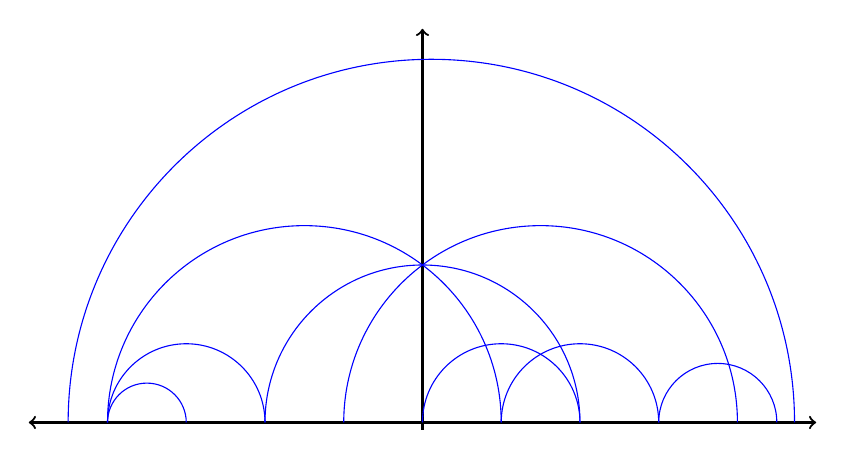
\begin{tikzpicture}
  \draw[color=black,thick,<->] (-5,0) -- (5,0);
  \draw[color=black,thick,<-] (0,5) -- (0,-0.1);

  \draw[blue] (2,0) arc (0:180:1);
  \draw[blue] (2,0) arc (0:180:2);
  \draw[blue] (3,0) arc (0:180:1);
  \draw[blue] (3,0) arc (180:0:0.75);
  \draw[blue] (-1,0) arc (180:0:2.5);
  \draw[blue] (-4,0) arc (180:0:2.5);
  \draw[blue] (-4,0) arc (180:0:0.5);
  \draw[blue] (-4,0) arc (180:0:1);
  \draw[blue] (-4.5,0) arc (180:0:4.6125);
\end{tikzpicture}

  \caption{Representación de algunas geodésicas en $\mathbb{H}^{2}$}
\end{figure}

Este ejemplo nos da lugar a enunciar el siguiente lema.

\begin{lemma}
  Las geodésicas en el espacio hiperbólico de dimensión $2$ son semi-rectas ortogonales al eje de las abscisas y semi-círculos con origen en el eje de las abscisas.
\end{lemma}

Los tres ejemplos que hemos dado son especialmente significativos, ya que, el \textit{Teorema de Killing$-$Hopf} nos dice que las variedades Riemannianas $n-$dimensionales, bajo ciertas restricciones, son isométricas a $\mathbb{R}^{n}$, $\mathbb{S}^{n}$ o $\mathbb{H}^{n}$, en el caso en que $n=2$ el \textit{Teorema de Uniformización} nos dice que toda variedad Riemanniana $2-$dimensional conexa es difeomorfa al cociente de algunas de las tres variedades anteriores modulo un grupo discreto de isometrías, las demostraciones de estos dos teoremas pueden ser consultadas en \textcite{lee2019introduction}.

% \section{Geodésicas en $\mathbb{D}^{2}$}

%
% % ====================================
% % Conclusiones
% % ====================================
%
% \chapter{Conclusiones}
\lipsum[1-3]

%
% % ====================================
% % Anexos
% % ====================================
%
% \appendix
\chapter{Topología de Variedades}\label{Anexo: Topologia De Variedades}
Estudiaremos algunas de las propiedades topológicas que poseen las variedades, mostraremos que la propiedad de ser segundo numerable y Hausdorff nos permite concluir que las variedades son paracompactas, más adelante veremos cómo esta propiedad nos permite garantizar la existencia de particiones suaves de la unidad, más aún, es posible mostrar que en una variedad suave existe una equivalencia entre paracompacidad, la existencia de particiones suaves de la unidad y que la variedad sea metrizable.

\begin{definition}[Espacio de Lindelöf]\label{Definición: Lindelöf}
  Sea $X$ un espacio topológico. Diremos que $X$ es un \it{espacio de Lindelöf} si cada cubierta abierta tiene una subcubierta numerable.
\end{definition}

\begin{theorem}
  Todo espacio topológico segundo numerable es un espacio de Lindelöf.
\end{theorem}

\begin{proof}
  Sea $X$ un espacio topológico segundo numerable y sea $\mathcal{U}$ una cubierta abierta de $X$. Por definición de espacio segundo numerable existirá una base numerable $\mathcal{B}$ para $X$.

  Definiremos el conjunto $\mathcal{B}' = \{B \in \mathcal{B} : B \subset U, U \subset \mathcal{U}\}$, esté conjunto es numerable dado que es un subconjunto de $\mathcal{B}$. Además, dado que $\mathcal{U}$ es una cubierta abierta de $X$, para cada $x \in X$ existirá un subconjunto abierto $U$ que contiene a $x$, y dado que $\mathcal{B}$ es base de $X$ por definición existe un elemento $B \in \mathcal{B}$ tal que $x \in B \subset U$, por lo tanto $B \in \mathcal{B}'$

  Ahora, para cada $B' \in \mathcal{B}'$ podemos tomar $U' \in \mathcal{U}$ tal que $B' \subset U'$. El conjunto formado por todos los elementos de esta forma es un subconjunto numerable de $\mathcal{U}$ y es una cubierta de $X$ dado que cada $x \in X$ está contenido en algún $B' \in \mathcal{B}'$.
\end{proof}

\begin{definition}[Subconjunto Precompacto]\label{Definición: Subconjunto Precompacto}
  Un subconjunto de un espacio topológico $X$ se dice que es \it{precompacto} en $X$ si su cerradura es compacta. 
\end{definition} 


\begin{definition}[Bolas Coordinadas Suaves]\label{Definición: Bolas Coordinadas Suaves}
  Sea $M^n$ una variedad suave, $(U,\phi)$ una carta suave de $M$. Diremos que $U$ es una \it{bola coordinada suave} si $\phi(U) \subset \R^n$ es una bola abierta de $\R^n$.
  
  Además, diremos que una bola coordinada suave $U \subseteq M$ es \it{regular} si existe una bola coordinada $U' \subseteq U$ y un mapa suave $\phi: U' \to \R^n$ tal que para algunos $r, r' \in \R^n$ se cumple:
  \[
    \phi(U) = B_r(U), \quad \phi(\overline{U}) = \overline{B}_r(0), \quad \phi(U') = B_{r'}(0)
  \] 
\end{definition}

\begin{lemma}\label{Lemma: Bolas Precompactas}
  Toda variedad topológica tiene una base numerable de bolas coordinadas precompactas.
\end{lemma}

\begin{proof}
  Sea $M^n$ una variedad topológica. Cada punto $p \in M$ está contenido en alguna carta $(U,\phi)$ por lo que las cartas forman una cubierta abierta para $M$; dado que $M$ es segundo numerable por definición de variedad topológica, y por el teorema anterior, se garantiza que existirá una subcubierta numerable de cartas $\{(U_i,\phi_i)\}$ para $M$.

  En el ejemplo \ref{Ex: Variedad Suave - Subvariedades Suaves} se mostró que los subconjuntos abiertos de una variedad topológica son en sí mismos variedades topológicas, por lo que el dominio de cada carta es una variedad topológica.

  Consideremos un elemento $(U,\phi)$ de la subcubierta numerable de cartas. Sabemos que una base numerable para la topología de $\R^n$ es el conjunto $\mathcal{B}$ formado por las bolas con radios y centros racionales, por el teorema de Heine-Borel la cerradura de cada una de estas bolas es un conjunto compacto por lo que las bolas son precompactas. Como $\phi$ es un homeomorfismo entre $U$ y $\R^n$, el conjunto $\phi^{-1} (\mathcal{B})= \{\phi^{-1}(B): B \in \mathcal{B}\}$ será una base para la topología de $U$ formado por una cantidad numerable de bolas coordinadas precompactas.

  Por lo tanto, el dominio de cada carta coordenada $U_i$ tiene una base de bolas coordenadas precompactas, y la unión de todas estas bases forma una base numerable de bolas precompactas en cada $U_i$ para la topología de $M$.
\end{proof}


Existe un resultado muy similar al anterior que funciona para variedades suaves, la demostración es idéntica, mutatis mutandis.

\begin{lemma}\label{Lemma: Base Por Bolas Suaves}
  Toda variedad suave tiene una base formada por una colección numerable de bolas coordinadas suaves.
\end{lemma}

Estos dos últimos lemas pueden ser generalizados a espacios topológicos si pedimos que el espacio tenga la siguiente propiedad.

\begin{definition}[Compacidad Local]
  Un espacio topológico $X$ se dice que es \it{localmente compacto} si cada punto tiene una vecindad contenida en un subconjunto compacto de $X$.
\end{definition}

\begin{corollary}
  Toda variedad topológica es localmente compacta.
\end{corollary}

\begin{lemma}
  Sea $X$ un espacio topológico de Hausdorff, segundo numerable y localmente compacto. Existe una base numerable y precompacta para $X$.
\end{lemma}

\begin{proof}
  Sea $X$ un espacio topológico y $\mathcal{B}$ una base numerable para $X$. Dado que $X$ es localmente compacto, para cada $x \in X$ existe una vecindad $U_x$ compacta, y dado que $X$ es un espacio de Hausdorff, la cerradura de $\overline{U_x}$ también es un conjunto compacto.

  Como $\mathcal{B}$ es una base de $X$, existirá un conjunto abierto $B \in \mathcal{B}$ tal que $x \in B \subseteq U_x$, es evidente que $\overline{B}$ es un conjunto cerrado en el compacto $\overline{U_x}$, por lo que $\overline{B}$ es compacto. Así, la colección formada por estos conjuntos con cerradura compacta es una base numerable y precompacta para $X$.
\end{proof}


\begin{definition}[Refinamiento]\label{Definición: Refinamiento}
  Sea $X$ un espacio topológico y sean $\mathcal{U}$ y $\mathcal{V}$ cubiertas de $X$. Diremos que $\mathcal{V}$ es un \it{refinamiento de $\mathcal{U}$} si para cada $V \in \mathcal{V}$ existe al menos un $U \in \mathcal{U}$ tal que $V \subseteq U$.
\end{definition}

\begin{definition}[Cubierta Localmente Finita y Paracompacidad]
  Sea $X$ un espacio topológico y $\mathcal{U}$ una cubierta abierta de $X$. Diremos que $\mathcal{U}$  es \it{localmente finita} si para cada $x$ existe una vecindad que interseca a lo más a un número finito de elementos de $U$.

  También diremos que $X$ es un \it{espacio paracompacto} si para cada cubierta abierta existe un refinamiento localmente finito. 
\end{definition}

\begin{theorem} [Espacios Precompactos] \label{Teorema: Espacios Precompactos}
 Sea $X$ un espacio de Hausdorff, segundo numerable y localmente compacto. $X$ es un espacio paracompacto.
\end{theorem}

\begin{proof}
  Sea $\mathcal{B}$ una base numerable para $X$ formada por conjuntos precompactos. Definimos la colección $\mathcal{A}$ del siguiente modo:
  \begin{align*}
    A_1 &= B_1\\
    &\vdots\\
    A_k &= B_1 \cup \dots \cup B_{j_k}
  \end{align*}

  Luego, sea $j_{k+1}$ el entero positivo más pequeño y mayor que $j_k$ tal que: $\overline{A_k} \subset \cup_{i=1}^{j_{k+1}} B_i$. Definimos al conjunto $A_{k+1}$ como
  \[
    A_{k+1} = \bigcup_{i=1}^{j_{k+1}} B_i
  \]

  Con esta definición la colección $\mathcal{A}$ es una secuencia definida de manera inductiva y tal que cada $A_i$ es un conjunto compacto, $\overline{A_i} \subset A_{i+1}$ y $X = \cup_{i=1}^{\infty} A_i$.

  Sea $\mathcal{U}$ una cubierta abierta de $X$. El conjunto $\overline{A_i} - A_{i-1}$ es compacto y por definición está contenido en el conjunto abierto $A_{i+1} - \overline{A_{i-2}}$. Para $i \geq 3$ podemos elegir una subcubierta finita de la cubierta abierta $\{U \cap (A_{i+1} - \overline{A_{i+2}}) : U \in \mathcal{U} \}$ del conjunto $\overline{A_{i}} - A_{i-1}$, y finalmente tomar una subcubierta finita de la cubierta abierta $\{U \cap A_3: U \in \mathcal{U}\}$ para el conjunto $\overline{A_2}$.

Esta colección de conjuntos es la unión numerable de colecciones finita de conjuntos por lo que será una colección numerable de refinamientos localmente finitos de la cubierta abierta $\mathcal{U}$, la cual consiste de conjuntos precompactos.
\end{proof}

\begin{corollary} \label{Corolario: Variedades Precompactas}
  Las variedades topológicas son paracompactas.
\end{corollary}

% \chapter{Álgebra Multilineal y Tensores}\label{Sección: Álgebra Multilineal y Tensores}

En este anexo describiremos lo que son los tensores, estos objetos nos darán una generalización del concepto de vector, además daremos un concepto básicas que necesitamos para entender a las métricas. Para comenzar necesitaremos dar algunas definiciones básicas de álgebra lineal.

\section{Álgebra Multilineal}
Comenzaremos definiendo a los anillos, estos son un tipo de estructura algebraica que generalizan el concepto de campo, en un anillo la multiplicación puede no ser asociativa y el inverso multiplicativo puede no existir para ningún elemento.

\begin{definition}[Anillo]
	Un \it{anillo} es un conjunto $\mathcal{R}$ junto con dos operaciones $(x,y) \to x + y$ y $(x,y) \to xy$, las cuales satisfacen las siguientes propiedades:
	\begin{itemize}
		\item $\mathcal{R}$ es un grupo conmutativo bajo la operación $(x,y) \to x + y$
		\item $(xy)z = x(yz)$
		\item $x(y + z) = xy + xz$ y $(y+z)x = yx + yz$
	\end{itemize}

	Si para cada $x,y \in \mathcal{R}$ se tiene que $xy = yx$, entonces diremos que $\mathcal{R}$ es un \it{anillo conmutativo} y, si existe un elemento $1 \in \mathcal{R}$ tal que $1x = x1 = x$ para cada $x \in \mathcal{R}$, entonces diremos que $\mathcal{R}$ es un \it{anillo con identidad}.
\end{definition}

Del mismo modo que como los anillos nos dan una generalización del concepto de campo, los módulos nos darán una generalización de los espacios vectoriales. La diferencia principal es que, mientras que los espacios vectoriales están definidos sobre un campo, los anillos estarán definidos sobre un anillo.

\begin{definition}[Módulo]
	Si $\mathcal{R}$ es un anillo con identidad. Diremos que un conjunto no vacío $\mathcal{M}$ es un \textit{$\mathcal{R}-$módulo} o un \it{módulo sobre $\mathcal{R}$} si:
	\begin{itemize}
		\item Hay una suma en $(\alpha,\beta) \to \alpha + \beta$ en $\mathcal{M}$ bajo la cual $\mathcal{M}$ es un grupo conmutativo.
		\item Hay un producto $(c,\alpha) \to c \alpha$, donde $\alpha \in \mathcal{M}$ y $c \in \mathcal{R}$
	\end{itemize}
	Para los cuales se cumplen las siguientes igualdades:
	\begin{gather*}
		\begin{alignedat}{2}
			(c_1 + c_2) \alpha                    & = c_1 \alpha + c_2 \alpha
			& \hspace{6em} c(\alpha_1 + \alpha_2) & = c\alpha_1 + c\alpha_2 \\
			c_1 c_2 \alpha                        & = c_1(c_2 \alpha)
			& 1 \alpha                            & = \alpha.
		\end{alignedat}
	\end{gather*}
\end{definition}
Como ya mencionamos, la principal diferencia entre los anillos y los campos es que, para los campos el inverso multiplicativo siempre está definido para todo elemento distinto de cero, esto no ocurre con los anillos, por lo cuál, los resultados de espacios que dependan de está propiedad no se trasladarán a los módulos; sin embargo, existen otros conceptos que sí podemos generalizar a los módulos.

\begin{definition}[Base Para Un Módulo]
	Si $\mathcal{M}$ es un $\mathcal{R}-$módulo, diremos que un subconjunto $\{m_i\}_{i \in I}$ es linealmente independiente si la igualdad:
	\[
		\sum_{i \in I} r_i m_i = 0, \quad r_i \in \mathcal{R},
	\]
	únicamente se cumple cuando todos los $r_i$ son nulos.

	Una \it{base} $\mathcal{B}$ para el módulo $\mathcal{M}$ es un subconjunto linealmente independiente que genera a $\mathcal{M}$, esto es, cada $m \in \mathcal{M}$ puede ser escrito como una combinación lineal:
	\[m = \sum_{i \in I} r_i m_i, \quad r_i \in \mathcal{R}.\]
	Para los módulos no es posible garantizar que si $\{m_i\}_{i \in I}$ es un conjunto linealmente dependiente entonces $m_j$ sea combinación lineal de los elementos del conjunto dado que la demostración de la proposición equivalente para espacios vectoriales hace uso del inverso multiplicativo; en consecuencia, tampoco podemos garantizar que todos los módulos tengan una base, como si ocurre con los espacios vectoriales, esto consecuencia del axioma de elección.
\end{definition}

\begin{definition}[Módulo Libre]
	Diremos que un $\mathcal{R}-$módulo $\mathcal{M}$ es un \it{módulo libre} si existe una base para $\mathcal{M}$, además si $\mathcal{M}$ tiene una base formada por un número finito de elementos diremos que $\mathcal{M}$ es un \it{módulo libre finito generado por $n$ elementos}.
\end{definition}

No es difícil mostrar que si $\mathcal{M}$ es un $\mathcal{R}-$módulo libre con $n$ generadores entonces el subconjunto más pequeño de $\mathcal{M}$ que lo genera contiene $n$ elementos, al número $n$ se le llama el \it{rango} del módulo. Está idea es similar a la de la dimensión de un espacio vectorial y como ocurre con los espacios vectoriales si $\mathcal{M}$ es un módulo libre generado por un número finito de elementos entonces habrá un isomorfismo canónico entre el módulo $\mathcal{M}$ y $\mathcal{R}^n$.

\begin{definition}[Módulo Dual]
	Si $\mathcal{M}$ es un $\mathcal{R}-$módulo definiremos al \it{módulo dual $\mathcal{M}^{*}$} como el conjunto de todas las funciones lineales $f: \mathcal{M} \to \mathcal{R}$.
\end{definition}

Los módulos duales son análogos a los espacios duales y comparten muchas de las mismas propiedades, de hecho, podemos mostrar que si $\mathcal{M}$ es finito generado entonces $\mathcal{M}^*$ también lo es, y la demostración de este teorema es exactamente igual a la demostración de que un espacio vectorial $V$ tiene la misma dimensión que su espacio dual $V^{*}$.

Ahora describiremos un tipo muy particular de mapa (en el sentido algebraico), los mapas multilineales, estos son mapas que son lineales en cada una de sus entradas. Algunos mapas multilineales deberían sernos familiares como el producto escalar en espacios euclidianos, el producto vectorial en $\R^3$ o las matrices.

\begin{definition}[Mapa Multilineal]
	Si $M, N$ y $P$ son $\mathcal{R}-$módulos diremos que un mapa:
	\[
		f: M \times N \to P
	\]
	es \it{bilineal} si $f$ es lineal en ambos factores, esto es:
	\begin{alignat*}{2}
		f(m_1 + m_2, n) & = f(m_1,n) + f(m_2,n),\quad  f(rm,n) & = rf(m,n) \\
		f(m, n_1 + n_2) & = f(m,n_1) + f(m,n_2),\quad  f(m,rn) & = rf(m,n) \\
	\end{alignat*}
	Del mismo modo, si $M_1, \ldots, M_n, P$ son $\mathcal{R}-$módulos, diremos una función:
	\[
		f: M_1 \times \cdots \times M_n \to P
	\]
	es \it{multilineal} si es es lineal en cada uno de sus factores, esto es:
	\begin{align*}
		f(m_1, \ldots, m_i^1 + m_i^2, \ldots, m_n) & = f(m_1, \ldots, m_i^2, \ldots, m_n)           \\
		                                           & \quad\quad +f(m_1, \ldots, m_i^2, \ldots, m_n) \\
		f(m_1,\ldots , rm_i, \ldots, m_n)          & = r f(m_1,\ldots,m_i,\ldots, m_n)
	\end{align*}
\end{definition}

A las funciones multilineales también se les conoce como \it{$n-$formas lineales}, una $1-$forma es simplemente una función lineal, una $2-$forma sería una función bilineal y así sucesivamente.

Como hemos mencionado, un ejemplo de un mapa bilineal es el producto escalar en $\R^n$, como recordatorio, el producto escalar es un mapa $\la \cdot , \cdot \ra: \R^n \times \R^n \to \R$ que definimos como:
\[
	\la x,y \ra = \sum_{i=1}^{n} x_i y_i, \quad\quad
	\begin{array}{l}
		x=[x_1,\dots,x_n] \in \R^n \\
		y=[y_1,\dots,y_n] \in \R^n
	\end{array}
\]
En la sección \ref{Sección: Variedades Riemannianas} extendemos la idea del producto escalar a variedades, esta es en gran parte la razón por la que estamos interesados en los mapas multilineales y los tensores ya que nos permiten realizar algunos cálculos importantes, como por ejemplo medir ángulos.
Otro ejemplo de un mapa multilineal además del producto escalar es el determinante. Dado que si tomamos $n+1$ vectores, $x_1, \ldots, x_n, y \in \R^n$ y un escalar $\lambda \in \R$, el determinante es un mapa que va de $\R^n \times \cdots \times \R^n$ a $\R^n$ para el cual se cumple:
\begin{align*}
	\det(\begin{bmatrix}x_1 & \cdots & \lambda x_i + y & \cdots & x_n \end{bmatrix}) = \lambda &
	\det(\begin{bmatrix}x_1 & \cdots &x_i&\cdots& x_n \end{bmatrix})                                                                                                  \\
	                                                                                           & + \det(\begin{bmatrix}x_1 & \cdots & y & \cdots & x_n \end{bmatrix})
\end{align*}

% \section{Productos Tensoriales}
\label{Sección: Productos Tensoriales}
Existen diferentes maneras de definir lo que, con los tensores, nosotros
estudiaremos en esta sección dos maneras de definirlos, cada una con sus
ventajas y desventajas; al final de esta sección probaremos que las dos
maneras son, esencialmente, equivalentes.

La primera definición que daremos es quizá la más sencilla, definiremos a los
tensores como mapas multilineales, la ventaja principal que nos da esta
definición es que podemos trabajar con los tensores con herramientas conocidas
del álgebra lineal y el cálculo; sin embargo, esto tiene la desventaja que las
representaciones de funciones multilineales dependen de las bases de los
espacios vectoriales.

\begin{definition}[Producto Tensorial de Mapas]
	Sean $V_1, \ldots, V_n$ y $W_1, \ldots, W_m$ espacios vectoriales sobre un
	campo $\K$, y sean $F \in L(V_1,\ldots,V_n;\K)$ y $G \in
		L(W_1, \ldots, W_m; \K)$. Definimos a la función:
	\[
		F \ot G:
		V_1 \times \cdots \times V_n \times W_1 \times \cdots \times W_m
		\to \K,
	\]
	como:
	\[
		F \ot G (v_1,\ldots,v_n,w_1,\ldots,w_m)
		= F(v_1,\ldots,v_n)G(w_1,\ldots,w_m).
	\]
\end{definition}
De la multilinealidad de $F$ y $G$ se sigue que $F \ot G$ depende
linealmente de cada uno de los vectores $v_1, \ldots, v_n, w_1, \ldots, w_m$,
por lo cual $F \ot G$ es un elemento de $L(V_1,\ldots,V_n,W_1,\ldots,W_m;
	\K)$, a esta función le llamamos el \textit{producto tensorial de $F$
	y $G$}.

Una consecuencia de que $F$ y $G$ sean elementos de $L(V_1,\ldots,V_n;
	\K)$ y $L(W_1,\ldots, W_m;\K)$ es que el producto tensorial es
un mapa bilineal y asociativo.

Mostraremos que el producto tensorial $\ot: L(V_i;\K) \times
	L(W_j; \K) \to \K$ es lineal en la primera coordenada, la
linealidad en la segunda coordenada se sigue exactamente de la misma manera.

Sean $F, G \in L(V_i;\K)$ y $H \in L(W_j;\K)$ y sean $(v_1,
	\ldots, v_n) \in V_1 \times \cdots \times V_n$, $(w_1, \ldots, w_n) \in W_1 \times
	\cdots \times W_m$ y $a \in \K$, para reducir un poco el tamaño de las
cuentas, denotaremos a los vectores $(v_1,\ldots,v_n)$ y $(w_1,\ldots,w_m)$
por $(v_i)$ y $(w_j)$, respectivamente. Por definición de producto tensorial
tenemos:
\begin{align*}
	(aF + G) \ot H ((v_i),(w_j)) & = (aF + G)(v_i) + H(w_j)                  \\
	                             & = \left[ aF(v_i) + G(v_i) \right] H(w_j)  \\
	                             & = aF(v_i)H(w_j) + G(v_i)H(w_j)            \\
	                             & = a(F \ot H)((v_i),(w_j))
	+ (G \ot H) ((v_i),(w_j))                                                \\
	                             & = (a (F \ot H) + (G \ot H)) ((v_i),(w_j))
\end{align*}

La asociatividad del producto tensorial es una consecuencia de la asociatividad
den el campo $\K$. Sean $V_1, \ldots, V_n$, $W_1,\ldots,W_m$, y $U_1,
	\ldots,U_p$ espacios vectoriales sobre un campo $\K$, y sean
$(v_1, \ldots, v_n) \in V_1 \times \cdots \times V_n$, $(w_1, \ldots, w_m)
	\in W_1 \times \cdots \times W_m$, $(u_1, \ldots, u_p) \in U_1 \times \cdots
	\times U_p$. Como se hizo anteriormente, abreviaremos a estos vectores
simplemente por $(v_i)$, $(w_j)$ y $(u_k)$ respectivamente.

Si $F \in L(V_i;\K)$, $G \in L(W_j;\K)$ y $H \in L(U_k;
	\K)$, tendremos que:
\begin{align*}
	(F \ot G) \ot H((v_i),(w_j),(u_k)) & = (F \ot G)((v_i),(w_j))H(u_k)       \\
	                                   & = \left[ F(v_i)G(w_j) \right] H(u_k) \\
	                                   & = F(v_i)\left[ G(w_j)H(u_k) \right]  \\
	                                   & = F(v_i)(G \ot H)((w_j),(u_k))       \\
	                                   & = F \ot (G \ot H)((v_i),(w_j),(u_k))
\end{align*}

La asociatividad del producto tensorial tiene una consecuencia muy interesante,
y es que, si tenemos $n$ funciones multilineales, $F_1, \ldots, F_n$, el
producto tensorial $F_1 \ot \cdots \ot F_n$ estará bien definido. Este hecho
nos permite enunciar el siguiente corolario.

\begin{corollary}
	Sean $V_1, \ldots V_n$ espacios vectoriales y $V_1^{*}, \ldots, V_{n}^{*}$
	sus espacios duales respectivos. Para cada vector $(v_1, \ldots, v_n) \in V_1
		\times \cdots \times V_n$ tenemos que el producto tensorial:
	\[
		\omega_1 \ot \cdots \ot \omega_n (v_1, \ldots, v_n)
		=
		\omega_1(v_1)\cdots \omega_n(v_n),
	\]
	donde cada $\omega_i$ es un covector arbitrario en $\in V_i^{*}$, para
	$1 \leq i \leq n$.
\end{corollary}

Gracias a este corolario es que podemos encontrar, de manera explícita, una
base para el espacio de funciones multilineales, como veremos con el siguiente
teorema.

\begin{theorem}[Base para el espacio de funciones multilineales]
	\label{Teorema: Base para el espacio de funciones multilineales}
	Sean $V_1, \ldots, V_k$ espacios vectoriales finito-dimensionales sobre un
	campo $\K$, con dimensiones $n_1, \ldots, n_k$ respectivamente. Para
	cada $1 \leq j \leq k$ sea $\{E_{1}^{j}, \ldots, E_{n_j}^{j} \}$ una base para el
	espacio $V_j$, y sea $\{\epsilon_{j}^{1}, \ldots, \epsilon_{j}^{n_j}\}$ la
	base correspondiente para el espacio dual $V_j^{*}$. El conjunto
	\[
		\mathcal{B} = \{\epsilon_{1}^{i_1} \ot \cdots \ot \epsilon_{k}^{i_k}
		: 1 \leq i_1 \leq n_1, \ldots, 1 \leq i_k \leq n_k\},
	\]
	es una base para el espacio $L(V_1,\ldots,V_k;\K)$.
\end{theorem}

\begin{proof}
	Demostraremos el caso para dos espacios vectoriales, el caso general se
	realiza exactamente de la misma manera.

	Sean $V$ y $W$ espacios vectoriales finito-dimensionales sobre un campo
	$\K$, con dimensiones $n$ y $m$ respectivamente, y sean $\{e_1,
		\ldots, e_n\}$ y $\{f_1, \ldots, f_n\}$ bases para $V$ y $W$. Para cada
	$1 \leq i \leq n$ y cada $1 \leq j \leq m$, definiremos las funciones
	multilineales $F_{ij} \in L(V,W;\mathbb{K})$ para las cuales:
	\[
		F_{ij} (v,w) = v_i w_j, \quad (v,w) \in V \times W,
	\]
	donde $v_i$ y $w_j$ son las $i-$ésimas y $j-$ésimas coordenadas de $v$ y $w$
	con respecto a las bases elegidas. Notemos que si $\{\epsilon^{1}, \ldots,
		\epsilon^{n}\}$ y $\{\phi^{1}, \ldots, \phi^{m}\}$ son las bases
	correspondientes  para los espacios duales $V^{*}$ y $W^{*}$, entonces,
	$F_{ij}$ coincide con el producto tensorial:
	\[
		\epsilon_{i} \ot \phi_{j} (v,w) = \epsilon_{i}(v) \phi_{j}(w)
		= u_{i}v_{j}.
	\]
	Mostraremos que el conjunto de funciones $F_{ij}$ es linealmente
	independiente, para esto tomemos $nm$ elementos del campo, digamos
	$\lambda_{1,1}, \ldots, \lambda_{n,m}$ y supongamos que $F_{ij} \in
		\ker\left(L(V,W;K)\right)$, esto quiere decir que para cada $(v,w) \in
		V \times W$ se tiene:
	\[
		\sum_{i=1}^{n}\sum_{j=1}^{m} \lambda_{i,j} F_{ij} = 0.
	\]
	En particular esto se cumple para los vectores de la base, por lo que:
	\[
		\sum_{i=1}^{n}\sum_{j=1}^{m}\lambda_{i,j}F_{i,j}(e_{\hat{\imath}}, f_{\hat{\jmath}})
		= \lambda_{\hat{\imath},\hat{\jmath}} = 0
	\]
	para cada $1 \leq \hat{\imath} \leq n$, $1 \leq \hat{\jmath} \leq m$, por lo cual, el
	conjunto es linealmente independiente.

	Ahora mostraremos que cada función multilineal $F \in L(V,W;\K)$
	se puede escribir como una combinación lineal de funciones $F_{i,j}$. Sea
	$F \in L(V,W;\K)$, para cada vector $(v,w) \in \K$ tenemos:
	\begin{align*}
		F(u,v) & = F\left(\sum_{i=1}^n v_i e_i,\sum_{j=1}^m w_j f_j \right) \\
		       & = F(v_1 e_1, w_1 f_1) + \cdots + F(v_n e_n, w_m f_m)       \\
		       & = F(e_1,f_1)v_1w_1 + \cdots + F(e_n,f_m) v_n w_m           \\
		       & = F(e_1,f_1)F_{1,1} + \cdots + F(e_n,f_m) F_{n,m}          \\
		       & = \sum_{i=1}^{n} \sum_{j=1}^{m} F_{i,j} F(e_i,f_j).
	\end{align*}
	Por lo tanto, podemos concluir que el conjunto de funciones $F_{ij}$ es
	una base para $L(V,W;\K)$, y, como ya hemos mencionado, estas
	funciones coinciden con el producto tensorial de los elementos de la base
	de los espacios duales.
\end{proof}

Ahora estudiaremos una segunda manera de definir a los tensores, esto será,
como elementos de un producto tensorial de espacios vectoriales. Como veremos
a continuación, esto tiene la ventaja de que los tensores no dependen de las
bases de los espacios vectoriales, por lo cual, este es un acercamiento libre
de coordenadas, sin embargo, esta manera de entender a los vectores también es
más abstracta.

Para poder hablar del producto tensorial de espacios vectoriales es necesario
que hablemos de la propiedad universal, a través de la cual definiremos al
producto tensorial.

\begin{definition}[La propiedad universal]
	Sean $V$ y $W$ espacios vectoriales y sea $\ot: V \times W \to T$, donde
	$T$ es algún espacio vectorial. Diremos que el mapa $\ot$ posee la
	\it{propiedad universal} si satisface las siguientes condiciones:
	\begin{enumerate}
		\item Los vectores $v \ot w$ generan a $T$, donde $v \in V$ y
		      $w \in W$.
		\item Si $\phi$ es algún mapa bilineal de $V \times W$ a cualquier espacio
		      vectorial $P$, entonces existe un mapa lineal único $f: T \to P$ que
		      hace que el diagrama \ref{Diagrama de la propiedad universal} sea
		      conmutativo.
	\end{enumerate}
\end{definition}

\begin{figure}[h]
	\center
	\tikzexternaldisable % Desactiva el precompilado de figuras, ¡No quitar!
\begin{tikzcd}
	V   \times W \arrow[d, "\otimes"'] \arrow[r, "\varphi"] & P \\[16pt]
	T \arrow[ru, "f"']                                        &
\end{tikzcd}
\tikzexternalenable % Restaura la el precompilado de figuras.

	\caption{Diagrama: Propiedad universal.}
	\label{Diagrama de la propiedad universal}
\end{figure}

Esta propiedad es universal en el sentido de que, dado dos espacios vectoriales
siempre existirá un tercer espacio vectorial y un mapa bilineal, único hasta
isomorfismo, que vaya del producto cartesiano de los dos espacios al tercer
espacio vectorial, el cual posea la propiedad universal. Nos gustaría esto, es
con este fin que demostraremos los siguientes lemas.

\begin{lemma}
	Sean $V, W$ y $T$ espacios vectoriales, $\ot: V \times W \to T$ un mapa
	bilineal que posee la propiedad universal, y sean $\{v_1,\ldots,v_n\}$ y
	$\{w_1,\ldots,w_n\}$ vectores linealmente independientes en $V$ y $W$
	respectivamente. La relación:
	\[
		\sum_{i=1}^{n} v_i \ot w_i = 0
	\]
	implica que $v_i = 0$ o que $w_i = 0$ para cada $1 \leq i \leq n$.
\end{lemma}

\begin{proof}
	Mostraremos que, si la relación se cumple, y los vectores $v_i$ no son
	necesariamente nulos, entonces cada $w_i$ debe ser nulo.

	Dado que los vectores $\{v_1,\ldots, v_n\}$ son linealmente independientes,
	podemos construir $n$ funciones $f_j: V \to \{0,1\}$ tales que:
	\[
		f_j (v_i) = \delta_{ij}
	\]
	También definiremos una función bilineal $\phi: V \times W \to P$, donde $P$
	es algún espacio vectorial. Definimos a $\phi$ de la siguiente manera:
	\[
		\phi(x,y) = \sum_{j=1}^{n} f_j(x)g_j(y), \quad x \in V, y \in W,
	\]
	donde $g_i$ son mapas lineales arbitrarios, definidos en $W$.

	Dado que $\ot$ posee la propiedad universal por hipótesis, existe un mapa
	lineal $f: T \to P$ tal que para cada $x \in V$ y cada $y \in W$ se tiene:
	\[
		f(x \ot y) = \phi(x,y) = \sum_{j=1}^{n} f_j(x)g_j(y)
	\]
	Si evaluamos el mapa $f$ en $\sum_{i=1}^{n} v_j \otimes w_j$ por la
	linealidad de $f$ y como hemos definido a las funciones $f_j$, se tendrá la
	siguiente cadena de igualdades.
	\begin{align*}
		f\l( \sum_{i=1}^{n} v_j \ot w_j \r)
		 & = \sum_{j=1}^{n} \l( \sum_{i=1}^{n} f_j(v_i) \ot g_j(w_i) \r) \\
		 & = \sum_{j=1}^{n} \sum_{i=1}^{n} \delta_{ij} g_j(w_i)          \\
		 & = \sum_{i=1}^{n} g_i(w_i) = 0
	\end{align*}
	Hemos dicho que las funciones $g_j$ son funciones lineales cualesquiera,
	por lo que podemos concluir que $w_i = 0$ para cada $1 \leq i \leq n$.
\end{proof}

\begin{lemma}
	Sea $\{e_\alpha\}_{\alpha \in A}$ una base para $V$, donde $A$ es algún
	conjunto indicador. Cada vector $z \in T$ puede ser escrito como:
	\[
		z = \sum_{\alpha} e_{\alpha} \ot w_{\alpha}, \quad w_{\alpha} \in W,
	\]
	donde a lo más, una cantidad finita de vectores $w_\alpha$ son no nulos.
	Los vectores $w_\alpha$ están determinados de manera única por el vector $z$.
\end{lemma}

\begin{proof}
	Dado que $\ot$ posee la propiedad universal, los elementos $x \otimes y$
	generan a $T$, lo cual implica que cada $z \in T$ puede ser escrito como la
	suma finita:
	\[
		z = \sum_{i=1}^{n} x_i \ot y_i, x_i \in V, y_i \in W.
	\]
	Expresaremos a cada $x_i$ como una combinación lineal de sus vectores bases,
	\[
		x_i = \sum_{\alpha}\lambda_{\alpha}^{i} e_\alpha,
		\quad
		\lambda_{\alpha}^{i} \in \K,
	\]
	de esta manera podemos escribir al vector $z$ como:
	\[
		z = \sum_{i=1}^{n}
		\l( \sum_{\alpha}\lambda_{\alpha}^{i} e_{\alpha} \r) \ot y_i,
	\]
	y dado que el mapa $\ot$ es bilineal la siguiente cadena de igualdades es
	verdadera:
	\begin{align*}
		z & = \sum_{\alpha}\sum_{i=1}^{n} \lambda_{\alpha}^{i} e_\alpha \ot y_i \\
		  & = \sum_{\alpha}\sum_{i=1}^{n} e_\alpha \ot \lambda_{\alpha}^{i} y_i \\
		  & = \sum_{\alpha} e_\alpha \ot \sum_{i=1}^{n}\lambda_{\alpha}^{i} y_i \\
		  & = \sum_{\alpha} e_\alpha \ot w_\alpha,
	\end{align*}
	esta última igualdad se obtiene simplemente de realizar la sustitución
	$w_\alpha = \sum_{i=1}^{n} \lambda_{\alpha}^{i} y_i$.

	Para probar la unicidad de los vectores $w_\alpha$ supongamos que existen
	vectores $\{w'_{\alpha}\}_{\alpha \in A}$ tales que:
	\[
		z = \sum_{\alpha} e_{\alpha} \ot w_\alpha
		= \sum_{\alpha} e_{\alpha} \ot w'_\alpha.
	\]
	Naturalmente esto implica que:
	\[
		\sum_{\alpha} e_{\alpha} \ot w_\alpha
		- \sum_{\alpha} e_{\alpha} \ot w'_\alpha = 0
	\]
	Y por la linealidad en la segunda coordenada del mapa $\ot$ obtenemos:
	\[
		\sum_{\alpha} e_{\alpha} \ot (w_{\alpha} - w'_{\alpha}) = 0
	\]
	Por el lema anterior podemos concluir que $w_{\alpha} = w'_{\alpha}$
	para cada $\alpha \in A$.
\end{proof}

\begin{lemma}
	Todo vector $z \in T$ puede ser escrito de la forma:
	\[
		z = \sum_{i=1}^{n} v_i \ot w_i, \quad v_i \in V, w_i \in W,
	\]
	donde $\{v_1,\ldots,v_n\}$ y $\{w_1,\ldots,w_n\}$ son vectores linealmente
	independientes.
\end{lemma}

\begin{proof}
	Sabemos que podemos representar a cada vector $z \in T$ como una suma finita
	\[
		z = \sum_{i=1}^{n} v_i \ot w_i.
	\]
	Nuestra intuición, al tener el vector una forma muy similar a la de una
	combinación lineal, debería decirnos que si $\{v_1, \ldots, v_n\}$a y
	$\{w_1, \ldots, w_n\}$ son linealmente independientes entonces $n$ debería
	ser el mínimo entero positivo para el cual es posible escribir a $z$ como
	una suma de esta forma.

	Elijamos pues, vectores $\{v_1,\ldots,v_n\}$ y $\{w_1,\ldots,w_n\}$ tales que
	$n$ sea minimizado.

	Si $n=1$, la independencia lineal se cumple trivialmente. Si por otra parte
	ocurre que $n \geq 2$ podemos proceder por contradicción. Supongamos que el
	conjunto $\{v_1, \ldots, v_n\}$ es linealmente independiente, si este es el
	caso, podemos suponer que:
	\[
		v_n = \sum_{i=1}^{n-1} \lambda_i v_i, \quad \lambda_{i} \in \K
	\]
	Por lo tanto, podremos escribir al vector $z$ como:
	\begin{align*}
		z & = \sum_{i=1}^{n} v_i \ot w_i                                        \\
		  & = \sum_{i=1}^{n-1} v_i \ot w_i + v_n \ot w_n                        \\
		  & = \sum_{i=1}^{n-1}v_i\ot w_i +\sum_{i=1}^{n-1}\lambda_i v_i \ot w_n \\
		  & = \sum_{i=1}^{n-1}v_i\ot (w_i + \lambda_i w_n)
		= \sum_{i=1}^{n-1} v_i \ot w'_i
	\end{align*}
	Pero esto querría decir que los vectores que hemos elegidos no minimizan a
	$n$, lo cual es una contradicción. Por lo tanto, los vectores $\{v_1,
		\ldots, v_n\}$ deben ser linealmente independientes.
	De manera análoga se demuestra que los vectores $\{w_1,\ldots, w_n\}$ son
	linealmente independientes.
\end{proof}

\begin{definition}[Producto tensorial de dos espacios vectoriales]
	Sean $V$ y $W$ espacios vectoriales. El \it{producto tensorial} de $V$ y $W$
	es un par $(T, \ot)$ donde $T$ es un espacio vectorial y $\ot: V \times W \to
		T$ es un mapa bilineal que posee la propiedad universal.
\end{definition}

\begin{theorem}
	Dado dos espacios vectoriales, su producto tensorial existe y es único hasta
	isomorfismo.
\end{theorem}

\begin{proof}
	Comenzaremos mostrando la unicidad. Sean $V$ y $W$ espacios vectoriales,
	supongamos que $(T,\ot)$ y $(T',\op)$ son productos tensoriales. Dado que
	tanto $\ot$ como $\op$ poseen la propiedad universal los siguientes diagramas
	serán conmutativos.
	\begin{figure}[h]
		\center
		\tikzexternaldisable % Desactiva el precompilado de figuras, ¡No quitar!
\begin{tikzcd}
	V \times W \arrow[r, "\oplus"] \arrow[d, "\otimes"'] & T' & V \times W
	\arrow[d, "\oplus"'] \arrow[r, "\otimes"] & T \\[12pt]
	T \arrow[ru, "f"']                                   &    & T' \arrow[ru, "g"']                                  &
\end{tikzcd}
\tikzexternalenable % Restaura la el precompilado de figuras.

	\end{figure}
	Por definición de la propiedad universal sabemos que tanto $f$ como $g$ son
	únicos hasta isomorfismo, así tendremos que $f\ot = \op$ y $g\op = \ot$. De
	aquí que $gf(\ot) = \ot = \id_{T}(\ot)$ y $fg(\op) = \op = \id_{T'}(\op)$,
	con lo cual podemos concluir que $gf =\id_{T}$ $fg = \id_{T'}$, por lo tanto
	$T \cong T'$.

	Ahora mostraremos la existencia. Consideremos el espacio generado por todas
	las combinaciones lineales formales de $V \times W$, denotaremos a este
	conjunto por $F(V \times W)$. Definiremos un subespacio de $F(V \times W)$,
	al cual denotaremos por $G(V \times W)$, este será el subespacio generado por
	todos los elementos de la forma:
	\begin{align*}
		(\lambda v_1 + \mu v_2, w) & - \lambda(v_1, w) - \mu(v_2, w) \\
		(v, \lambda w_1 + \mu w_2) & - \lambda(v, w_1) - \mu(v, w_2) \\
	\end{align*}
	Sean $T$ el espacio cociente $F(V \times W) / G(V \times W)$ y $\pi:
		F(V \times W) \to T$ el mapa proyección. Definiremos el mapa $\ot: V
		\times W \to T$ como:
	\[ v \times w = \pi(v,w) \]
	Mostraremos que $\ot$ posee la propiedad universal. Claramente el mapa $\ot$
	es bilineal, para mostrar que los vectores $v \ot w$ generan a $T$ observemos
	que, por los resultados mostrados anteriormente, cada vector $z \in T$ puede
	ser escrito como una suma finita:
	\[ z = \pi \l(\sum_{i=1}^n\sum_{j=1}^{n} \lambda_{ij}(v_i,w_j)\r) \]
	Por lo tanto, se sigue que:
	\[
		z = (\sum_{i=1}^n\sum_{j=1}^{m} \lambda_{ij}\pi(v_i,w_j)
		= \sum_{i=1}^n\sum_{j=1}^{m} \lambda_{ij} v_i \times w_j,
	\]
	por lo cual, $T$ es generado por los vectores $v \ot w$.

	Ahora, para mostrar la segunda condición consideremos un espacio vectorial
	$P$ y un mapa bilineal $\phi: V \times W \to P$. Podemos extender $\phi$ a
	un mapa lineal $g: F(V \times W) \to P$ definiendo:
	\[
		g\l(\sum_{i=1}^{n}\sum_{j=1}^{m}\lambda_{ij} (v_i,w_j)\r)
		=
		\sum_{i=1}^{n}\sum_{j=1}^{m} \lambda_{ij}f(v_i,w_j)
	\]
	Notemos que para cada $z \in G(V \times W)$ se tendrá que $g(z) = 0$, esto
	dado que si $z$ es un elemento generador de $G(V \times W)$, entonces:
	\begin{align*}
		g(z) & = g((\lambda v_1 + \mu v_2, w) - \lambda(v_1,w)   -\mu(v_2,w))    \\
		     & = g(\lambda v_1 + \mu v_2,  w) - \lambda g(v_1,w) -\mu g(v_2,w)   \\
		     & = \phi(\lambda v_1+\mu v_2, w) -\lambda\phi(v_1,w)-\mu\phi(v_2,w) \\
		     & = 0
	\end{align*}
	Se concluye que $G(V \times W) \subset \ker(g)$, por lo cual $g$ debe inducir un mapa
	lineal
	\[ f: F(V \times W) / G (V \times W) \to P, \]
	tal que:
	\[
		f \circ \pi = g.
	\]
	Esto muestra que:
	\[
		(f \circ \ot)(v,w) = g(v,w) = \phi(v,w)
	\]
	Así, $\otimes$ posee la propiedad universal, por lo cual $(T, \ot)$ es el
	producto tensorial de $V$ y $W$.
\end{proof}

La idea del producto tensorial de espacios vectoriales puede ser extendida de
manera muy natural al producto de $n$ espacios vectoriales, al igual que ocurre
en el caso de dos espacios, este producto tensorial siempre existe y es único
hasta isomorfismo, la demostración se realiza de la misma manera.

\begin{definition}[Propiedad universal]
	Sean $V_1, \ldots, V_n$ espacios vectoriales y $\ot: V_1 \times \cdots \times
		V_n \to T$ un mapa multilineal. Diremos que el mapa $\ot$ posee la propiedad
	universal si:
	\begin{itemize}
		\item Los vectores $v_1 \ot\cdots\ot v_n$ genera a $T$, donde $v_i\in V_i$.
		\item Cada mapa multilineal $\phi: V_1 \times \cdots \times V_n \to P$,
		      donde $P$ es un espacio vectorial, puede ser escrito de la forma:
		      \[ \phi(v_1,\ldots,v_n) = f(v_1 \otimes \cdots \otimes v_n), \]
		      donde $f: T \to P$ es un mapa lineal.
	\end{itemize}
\end{definition}

\begin{definition}[Producto tensorial de espacios vectoriales]
	Sean $V_1, \ldots, V_n$ espacios vectoriales, el \it{producto tensorial} de
	$V_1,\ldots,V_n$ es un par $(T, \ot)$, donde $\ot: V_1 \times \cdots \times
		V_n \to T$ es un mapa multilineal que posee la propiedad universal. Usualmente
	nos referimos simplemente a $T$ como el producto tensorial de los espacios
	vectoriales y denotamos a $T$ como $V_1 \ot \cdots \ot V_n$.
\end{definition}

\begin{theorem}[Base para el producto tensorial de espacios vectoriales]
	\label{Teorema: Base para el producto tensorial}
	Sean $V_1, \ldots, V_k$ espacios vectoriales finito-dimensionales, con
	dimensiones $n_1, \ldots, n_k$, respectivamente. Para cada $1 \leq j \leq k$,
	supongamos que $\{E_{1}^{j}, \ldots E_{n_j}^{j}\}$ es una base para $V_j$.
	Entonces, una base para el producto tensorial $V_1 \ot \cdots \ot V_k$ es
	el conjunto:
	\[
		\mathcal{C} = \{ E_{i_1}^{1} \ot \cdots \ot E_{i_k}^{k} :
		1 \leq i_1 \leq n_1, \ldots, 1 \leq i_n \leq n_k \}
	\]
\end{theorem}

\begin{proof}
	Mostraremos el caso para el producto tensorial de dos espacios vectoriales.
	Sean $V$ y $W$ espacios vectoriales, $\{v_1,\ldots,v_n\}$ y $\{w_1,\ldots,
		w_n\}$ bases para $V$ y $W$ respectivamente, como hemos visto, cada vector
	$(v \otimes w) \in V \otimes W$ puede ser expresado como:
	\[
		v \ot w = \sum_{i=1}^{n}\sum_{j=1}^{m} \lambda_i \mu_j v_i \ot w_j,
		\quad \lambda_i, \mu_j \in \K
	\]
	donde los escalares $\lambda_i$ y $\mu_j$ están determinados de forma única
	por la representación de $v$ y $w$ como combinaciones lineales:
	\[
		v = \sum_{i=1}^{n} \lambda_i v_i, \quad w = \sum_{j=1}^{n} \mu_i w_i
	\]

	Ahora mostraremos que el conjunto de vectores $\{v_i \otimes w_j\}$ es
	linealmente independiente. Procederemos de modo similar a como se hizo en la
	demostración del teorema \ref{Teorema: Base para el espacio de funciones
		multilineales}.

	Para cada $1 \leq i \leq n$ y cada $1 \leq j \leq m$ definiremos $n m$
	bilineales $\Phi_{i j}: V \times W \to \K$, estas funciones estarán dadas por:
	\[
		\Phi_{ij}(x,y) = x_i y_j, \quad x \in V, y \in W,
	\]
	donde $x_i$ e $y_j$ son las $i-$ésima y $j-$ésimas coordenadas de $x$ e $y$
	con respecto a las bases elegidas. Dado que cada uno de los mapas $\Phi_{ij}$ es
	bilineal y que el mapa $\ot$ posee la propiedad universal, existirán $nm$
	funciones lineales tales que:
	\[
		\phi_{ij}(v \ot w) = \Phi_{ij}(v,w)
	\]
	Al evaluar cada una de estas funciones $\phi_{ij}$ en cualquier vector del
	kernel, digamos:
	\[
		\sum_{i=1}^{n}\sum_{j=1}^{m} \lambda_i \mu_j (v_i \otimes w_j) = 0,
	\]
	obtendremos que:
	\begin{align*}
		\phi_{\hat{\imath}\hat{\jmath}}\l(\sum_{i=1}^{n}\sum_{j=1}^{m}\lambda_i\mu_j(v_i \ot w_j)\r)
		 & = \sum_{i=1}^{n}\sum_{j=1}^{m}\lambda_i\mu_j\phi_{\hat{\imath}\hat{\jmath}}(v_i\ot w_j) \\
		 & = \sum_{i=1}^{n}\sum_{j=1}^{m}\lambda_i\mu_j\Phi_{\hat{\imath}\hat{\jmath}}(v_i,w_j)
		= \lambda_{\hat{\imath}} \mu_{\hat{\jmath}} = 0
	\end{align*}
	Por lo tanto, podemos concluir que el conjunto de vectores $v_i \ot w_j$ es
	linealmente independiente, y por lo tanto forman una base para $V \ot W$.
\end{proof}

Para terminar con esta sección probaremos la afirmación que hicimos al
principio, que ambas maneras de definir a los tensores, tanto como funciones
multilineales como elementos de productos tensoriales son esencialmente
equivalentes.

\begin{theorem}
	\label{Teorema: Isomorfismo Entre Tensores y Funciones}
	Si $V_1, \ldots, V_n$ son espacios vectoriales sobre un campo $\K$, entonces,
	existen isomorfismos canónicos:
	\[ V_1^* \ot \cdots \ot V_n^* \cong L(V_1, \ldots, V_n; K) \]
	y
	\[ V_1 \ot \cdots \ot V_n \cong L(V_1^*, \ldots, V_n^*; K) \]
\end{theorem}

\begin{proof}
	Realizaremos la demostración para el primer isomorfismo, el segundo
	isomorfismo se sigue de manera similar.

	Sea $\phi: V_1^{*} \times \cdots \times V_n^{*} \to L(V_1, \ldots ,V_n; \K)$
	la función multilineal definida por la relación:
	\[
		\phi(\omega_1,\ldots,\omega_n)(v_1,\ldots,v_n)
		=
		\omega(v_1)\cdots\omega(v_n)
	\]
	Por la propiedad universal de los productos tensoriales sabemos que debe
	existir una función lineal única $f: V_1 \ot \cdots \ot V_n \to L(V_1, \ldots
		V_n; K)$ para el cual, el diagrama \ref{Diagrama: Isomorfismo entre el
		producto tensorial y el espacio de funciones multilineales} es conmutativo.
	\begin{figure}[h]
		\center
		\tikzexternaldisable % Desactiva el precompilado de figuras, ¡No quitar!
\begin{tikzcd}
	V_{1}^{*} \times \cdots \times V_{n}^{*} \arrow[rd, "\otimes"', shift right]
	\arrow[rr, "\varphi"] &
	& {L(V_1,\ldots ,V_n; \mathbb{K})} \\[24pt]
	& V_{1}^{*} \otimes \cdots \otimes V_{n}^{*} \arrow[ru, "f"'] &
\end{tikzcd}
\tikzexternalenable % Restaura la el precompilado de figuras.

		\caption{Diagrama: Isomorfismo entre el producto tensorial y el espacio de
			funciones multilineales.}
		\label{Diagrama: Isomorfismo entre el
			producto tensorial y el espacio de funciones multilineales}
	\end{figure}
	Esto quiere decir que para cada $(v_1, \ldots, v_n) \in V_1 \times \cdots
		\times V_n$ tendremos:
	\[
		f(\omega_1 \ot \cdots \ot \omega_n)(v_1,\ldots,v_n)
		=
		\omega_1(v_1) \cdots \omega_n(v_n)
	\]
	Esta función será un isomorfismo entre los espacios vectoriales $V_1 \ot
		\cdots \ot V_n$ y $L(V_1,\ldots,V_n; \K)$, dado que es lineal, inyectiva para
	cada vector $(v_1, \ldots, v_n) \in V_1 \times \cdots \times V_n$ y que, como
	vimos con los teoremas \ref{Teorema: Base para el espacio de funciones
		multilineales} y \ref{Teorema: Base para el producto tensorial}, ambos
	espacios tienen la misma dimensión, a saber, su dimensión es el producto de
	cada una de las dimensiones de los espacios vectoriales $V_1, \ldots, V_n$.
\end{proof}

Gracias a este teorema podemos referirnos de manera indistinta a los espacios
$L(V_1,\ldots,V_n;K)$ y $V_1^* \ot \cdots \ot V_n^*$ de manera indistinta, y
únicamente haremos la distinción si es que es necesario.

% \section{Clasificación de Tensores}
\label{Sección: Clasificación de Tensores}
Ahora que sabemos que son los productos tensoriales podemos hablar de sus
elementos, los tensores. En esta sección daremos algunas definiciones que
nos permitirán clasificarlos de una manera que nos es útil.

\begin{definition}[Tensores covariantes, contravariantes y mixtos]
	Sea $V$ un espacio vectorial sobre un campo $\K$, y sean $k$ y $l$ enteros no
	negativos. Diremos que:
	\begin{enumerate}
		\item Una función multilineal $\alpha: V^{k} \to \K$ es un \it{tensor
			      covariante de rango $k$} o un \it{$k-$tensor covariante}.
		      Denotaremos al conjunto de tensores contravariantes de rango $k$ por
		      $\mathfrak{T}^k(V)$.
		\item Una función multilineal $\alpha: (V^l)^* \to \K$ es un \it{tensor
			      contravariante de rango $l$} o un \it{$l-$tensor contravariante}.
		      Denotaremos al conjunto de tensores contravariantes de rango $l$ por
		      $\mathfrak{T}_l(V)$.
		\item Una función multilineal $\alpha: V^k \times (V^l)^* \to \K$ es un
		      \it{$(k,l)-$tensor} o un \it{tensor mixto de tipo $(k,l)$}.
		      Denotaremos al conjunto de todos los tensores de tipo $(k,l)$ por
		      $\mathfrak{T}_{l}^{k}(V)$.
	\end{enumerate}
\end{definition}

\begin{example}
	Algunos tensores, tanto covariante, como contravariantes y de rango mixto ya
	nos son familiares. Mencionaremos algunos de ellos.
	\begin{itemize}
		\item Los $0-$tensores, tanto covariantes como contravariantes son
		      simplemente escalares del campo.
		\item Las formas bilineales son, por definición, $2-$tensores covariantes.
		      Más en general, una forma $k-$lineal es un $k-$tensor covariante.
		\item El producto escalar de dos vectores en $\R^{n}$ es un $2-$tensor
		      covariante.
		\item El diferencial de un mapa es un $l-$tensor contravariante, donde $l$
		      es la dimensión de la variedad suave sobre la cual definimos al mapa.
		\item Todo endomorfismo es un $(1,1)-$tensor. De hecho, existe un
		      isomorfismo entre el conjunto de endomorfismo de un espacio
		      vectorial,
		      $\mathrm{End}(V)$, y el conjunto de tensores mixtos de tipo $(1,1)$,
		      $\mathfrak{T}_{1}^{1}(V)$.
	\end{itemize}
\end{example}

No es difícil ver que los tensores mixtos que hemos definido son una
generalización de los tensores covariantes y de los tensores contravariantes,
podemos dar algunas relaciones que son verdaderas para estos espacios.
\begin{align*}
	\mathfrak{T}_{0}^{0}(V) & = \mathfrak{T}^{0}(V) = \mathfrak{T}_{0}(V) = \K \\
	\mathfrak{T}_{0}^{1}(V) & = \mathfrak{T}^{1}(V) = V                        \\
	\mathfrak{T}_{1}^{0}(V) & = \mathfrak{T}_{0}(V) = V^{*}                    \\
	\mathfrak{T}_{k}^{0}(V) & = \mathfrak{T}^{k}(V)                            \\
	\mathfrak{T}_{l}^{0}(V) & = \mathfrak{T}_{l}(V)
\end{align*}

Por el teorema \ref{Teorema: Isomorfismo Entre Tensores y Funciones} sabemos que
el espacio de tensores mixtos $\mathfrak{T}_{l}^{k}(V)$ debe ser isomorfo al
producto tensorial de $V^k$ con $(V^l)^*$, esto es,
\[
	\mathfrak{T}_{l}^{k}(V) \cong \underbrace{V \ot \cdots \ot V}_{k-\text{veces}}
	\ot \underbrace{V^* \ot \cdots \ot V^*}_{l-\text{veces}}
\]
es por este isomorfismo y las relaciones dadas anteriormente que podemos
enunciar el siguiente corolario, el cual nos describe, de manera explícita, las
bases para los espacios de tensores.

\begin{corollary}
	Sea $V$ un espacio vectorial $n-$dimensional. Sean $\{E_1, \ldots, E_n\}$ una
	base para $V$ y $\{\epsilon_1, \ldots, \epsilon_n\}$ una base para el espacio
	dual $V^{*}$, no necesariamente la base correspondiente. Entonces:
	\begin{itemize}
		\item Una base para el espacio de $k-$tensores covariantes
		      $\mathfrak{T}^{k}(V)$ es el conjunto:
		      \[
			      \{\epsilon^{i_1} \ot \cdots \ot \epsilon^{i_k}: 1 \leq i_1 ,\ldots,
			      i_k \leq n\}
		      \]
		\item Una base para el espacio de $l-$tensores contravariantes
		      $\mathfrak{T}_l(V)$ es el conjunto:
		      \[
			      \{E_{i_1} \ot \cdots \ot E_{i_l}: 1 \leq i_1, \ldots, i_l \leq n\}
		      \]
		\item Una base para el espacio de tensores mixtos de tipo $(k,l)$,
		      $\mathfrak{T}_{l}^{k}(V)$, es el conjunto:
		      \[
			      \{E_{i_1} \ot \cdots \ot E_{i_k} \ot \epsilon_{j_1} \ot \cdots \ot
			      \epsilon_{j_l}: 1 \leq i_1, \ldots, i_k \leq n, 1 \leq j_1, \ldots,
			      j_l \leq n\}
		      \]
	\end{itemize}
\end{corollary}

Esta clasificación que hemos dado para los elementos de los productos tensoriales
nos está hablando acerca de los espacios vectoriales sobre los cuales estamos
definiendo estos tensores. Ahora veremos otra manera de clasificarlos, la cual
no es mutuamente exclusiva con la clasificación que acabamos de dar, esta
manera de clasificar a los tensores nos dirá como es que estos se comportan
cuando sus argumentos son reordenados.

\begin{definition}[Tensores simétricos y antisimétricos]
	Sea $V$ un espacio vectorial y $\alpha$ un tensor covariante en $T^{k}(V)$.
	Diremos que:
	\begin{itemize}
		\item $\alpha$ es un \it{tensor simétrico} si para cualquier conjunto de
		      vectores $v_1, \ldots, v_k \in V$ y cualquier par de índices $1 \leq i
			      \leq j \leq k$ se cumple que:
		      \[
			      \alpha(v_1,\ldots,v_i,\ldots,v_j,\ldots,v_k) =
			      \alpha(v_1,\ldots,v_j,\ldots,v_i,\ldots,v_k)
		      \]
		\item $\alpha$ es un \it{tensor antisimétrico} si para cualquier conjunto de
		      vectores $v_1, \ldots, v_k \in V$ y cualquier par de índices $1 \leq i
			      \leq j \leq k$ se cumple que:
		      \[
			      \alpha(v_1,\ldots,v_i,\ldots,v_j,\ldots,v_k) =
			      -\alpha(v_1,\ldots,v_j,\ldots,v_i,\ldots,v_k)
		      \]
	\end{itemize}
\end{definition}

Estamos interesados particularmente en los tensores simétricos, ya que, uno de
nuestros objetivos principales es el estudiar el tensor de Riemann, el cual se
define como un tensor simétrico, sin embargo, los tensores antisimétricos
también son muy importantes; es posible mostrar que cualquier $2-$tensor
covariante puede ser escrito como la suma de un tensor simétrico y un tensor
antisimétrico.

El conjunto de todos los tensores simétricos en el espacio $\mathfrak{T}^{k}(V)$
es un subespacio de este, al subespacio formado por los tensores
simétricos en $\mathfrak{T}^{k}(V)$ lo denotaremos por $\Sigma^{k}(V)$. A
continuación, demostraremos algunas de las propiedades que se cumplen para estos 
tensores.

Recordemos que una \it{permutación} en un conjunto $A = \{1, \ldots, k\}$ es
una biyección $\sigma: A \to A$; al conjunto de todas las permutaciones
en un conjunto de $k$ elementos le llamamos el \it{grupo de simetrías de $k$
	símbolos} y lo denotamos por $S_k$.

\begin{definition}[Simetrización de un tensor]
	Dados un $k-$tensor covariante $\alpha$ y una permutación $\sigma \in S_{k}$,
	definiremos al $k-$tensor covariante $\sigma(\alpha)$ como:
	\[
		\sigma(\alpha)(v_1,\ldots,v_k) = \alpha(v_{\sigma(1)},\ldots,v_{\sigma(k)}).
	\]
	Definimos la función $\mathrm{Sym}: \mathfrak{T}^k(V) \to \Sigma^{k}(V)$ como
	la función:
	\[
		\mathrm{Sym}(\alpha) = \frac{1}{k!} \sum_{\sigma \in S_{k}} \sigma(\alpha).
	\]
	A esta función le llamamos la \it{simetrización} de $\alpha$.
\end{definition}

\begin{lemma}
	Sea $\alpha$ un $k-$tensor covariante en $\mathfrak{T}^{k}(V)$, donde $V$ es un
	espacio vectorial finito-dimensional. Las siguientes afirmaciones son
	verdaderas.
	\begin{itemize}
		\item $\mathrm{Sym}(\alpha) = \alpha$ si y solo si $\alpha$ es simétrico.
		\item $\mathrm{Sym}(\alpha)$ es un tensor simétrico.
	\end{itemize}
\end{lemma}

\begin{proof}
	Comencemos notando que $\alpha$ es un $k-$tensor simétrico si y solo si
	para cualquier permutación $\sigma \in S_{k}$ se tiene que:
	\[
		\alpha(v_1, \ldots, v_k) = \sigma (\alpha(v_1, \ldots, v_k)) =
		\alpha(v_{\sigma(1)}, \ldots, v_{\sigma(k)}),
	\]
	esto dado que, por definición, un tensor es simétrico si y solo si permanece
	invariante bajo cualquier transposición y que cada permutación puede ser
	expresada como el producto de ciclos.

	De este hecho se sigue inmediatamente la primera proposición dado
	que si $\alpha$ es simétrico, entonces, será igual a cualquiera de sus
	permutaciones y dado que hay $k!$	permutaciones en $S_k$, obtenemos:
	\[
		\alpha = \mathrm{Sym}(\alpha) = \frac{1}{k!} \sum_{\sigma \in
			S_{k}} \sigma(\alpha)
	\]
	Del mismo hecho también es posible deducir que $\mathrm{Sym}(\alpha)$ es un
	tensor simétrico, dado que si $\tau$ es cualquier permutación en
	$S_{k}$, el producto $\tau \sigma$ también es una permutación en
	$S_k$, y, por lo tanto:
	\begin{align*}
		\tau(\mathrm{Sym}(\alpha))
		 & = \tau \l( \frac{1}{k!} \sum_{\sigma\in S_k} \sigma(\alpha) \r) \\
		 & = \frac{1}{k!} \sum_{\sigma \in S_k} \tau\sigma(\alpha)         \\
		 & = \frac{1}{k!} \sum_{\mu \in S_k} \mu(\alpha)                   \\
		 & = \mathrm{Sym}(\alpha)
	\end{align*}
\end{proof}

En general, dados dos tensores covariantes $\alpha \in \mathfrak{T}^{k}(V)$ y
$\beta \in \mathfrak{T}^{l}(V)$ su producto tensorial, $\alpha \ot \beta$ no
será simétrico, de hecho, no es posible garantizar esto ni siquiera cuando
$\alpha$ y $\beta$ son tensores simétricos; sin embargo, utilizando la función
de simetrización definida anteriormente, podemos definir un nuevo producto, al
cual, por el lema anterior podemos garantizar es simétrico.

Si $\alpha$ es un $k$-tensor covariante simétrico y $\beta$ es un $l-$tensor
covariante simétrico, definimos el \it{producto simétrico de $\alpha$ y
	$\beta$}, al cual denotaremos por $\alpha \beta$ como el $(k+l)$-tensor
covariante dado por
\[
	\alpha \beta = \mathrm{Sym}(\alpha \ot \beta)
\]
Podemos ser más explícitos con esta definición, recordando como hemos definido el
producto tensorial de funciones multilineales al inicio de la sección pasada
y utilizando la definición que hemos dado para el producto simétrico, podemos
decir que al aplicar el producto simétrico $\alpha \beta$ sobre vectores
$v_1, \ldots, v_k, v_{k+1}\ldots, v_{k+l} \in V$, su representación será:
\[
	\alpha \beta(v_1, \ldots, v_k, v_{k+1}, \ldots, v_{k+l})
	=
	\frac{1}{(k+l)!}
	\sum_{\sigma \in S_{k+l}}
	\alpha(v_{\sigma(1)}, \ldots, v_{\sigma(k)})
	\beta(v_{\sigma(k+1)}, \ldots, v_{\sigma(k+l)})
\]

\begin{lemma}
	El producto simétrico es bilineal, esto quiere decir que, si $\alpha$,
	$\beta$ y $\gamma$ son tensores covariantes en $\mathfrak{T}^{k}(V)$,
	$\mathfrak{T}^{l}(V)$ y $\mathfrak{T}^{m}(V)$ respectivamente, y $a$ y $b$ son
	escalares en $\mathbb{K}$, entonces
	\[
		(a \alpha + b \beta)\gamma = a \alpha \gamma + b \beta \gamma
	\]
\end{lemma}

\begin{proof}
	El producto simétrico es bilineal dado que el producto tensorial de funciones
	multilineales lo es, por definición tenemos:
	\begin{align*}
		(a\alpha + b\beta) \gamma
		 & = \Sym ((a \alpha + b \beta)\ot \gamma)              \\
		 & = \Sym (a(\alpha \ot \gamma) + b(\beta \ot \gamma)),
	\end{align*}
	por definición de la función de simetrización tendremos que:
	\begin{align*}
		(a \alpha + b \beta)\gamma
		 & = \frac{1}{(k+l+m)!} \sum_{\sigma \in S_{k+l+m}}
		a \sigma(\alpha) \sigma(\gamma) + b \sigma(\beta) \sigma(\gamma) \\
		% Segunda linea
		 & = \frac{a}{(k+l+m)!} \sum_{\sigma \in S_{k+l+m}}
		\sigma(\alpha) \sigma(\gamma)
		+ \frac{b}{(k+l+m)!} \sum_{\sigma \in S_{k+l+m}}
		\sigma(\beta) \sigma(\gamma)                                     \\
		% Tercera linea
		 & = \frac{a}{(k+m)!} \sum_{\sigma \in S_{k+m}}
		\sigma(\alpha) \sigma(\gamma)
		+ \frac{b}{(l+m)!} \sum_{\sigma \in S_{l+m}}
		\sigma(\beta) \sigma(\gamma)                                     \\
		 & = a\Sym(\alpha \ot \gamma) + b\Sym(\beta \ot \gamma)          \\
		 & = a \alpha \gamma + b \beta \gamma
	\end{align*}
\end{proof}

\begin{lemma}\label{Lema: Descomposición de Tensores}
	Si $\alpha$ y $\beta$ son $1-$tensores covariantes, entonces:
	\[
		\alpha \beta = \frac{1}{2} \l(\alpha \ot \beta + \beta \ot \alpha \r)
	\]
\end{lemma}

\begin{proof}
	Si $\alpha$ y $\beta$ son $1-$tensores covariantes, entonces por definición
	son simplemente funciones lineales, por definición del producto simétrico se
	tiene:
	\begin{align*}
		\alpha \beta
		 & = \Sym(\alpha \ot \beta)
		= \Sym \l(\frac{1}{2} \alpha \ot \beta + \frac{1}{2} \alpha \ot \beta \r) \\
		 & = \frac{1}{2} \alpha \beta + \frac{1}{2} \alpha \beta
		= \frac{1}{2} \l( \alpha \beta + \beta \alpha \r)                         \\
		 & = \frac{1}{2} \l( \alpha \ot \beta + \beta \ot \alpha \r)
	\end{align*}
\end{proof}

% \section{Campos Tensoriales}\label{Sección: Campos Tensoriales}


% \chapter{Corchetes de Lie}\label{Anexo: Corchetes de Lie}
\begin{definition}[Corchete de Lie]
	Si $X$ e $Y$ son campos vectoriales suaves en una variedad $M$. Definimos al campo vectorial $[X,Y]$ como:
	\[
		[X,Y]f = X(Yf) - Y(Xf),
	\]
	donde $f$ es una función suave en $C^{\infty}(M)$. Al campo vectorial $[X,Y]$ le llamamos el \textit{corchete de Lie}.
\end{definition}

\begin{lemma}
	Si $X$ e $Y$ son campos vectoriales suaves. Entonces, el corchete de Lie $[X,Y]$ cumple las siguientes propiedades:
	\begin{itemize}
		\item $[X,Y]$ es un campo vectorial suave en $M$.
		\item El corchete de Lie es un mapa bilineal.
		\item El corchete de Lie es anticonmutativo.
		\item Si $f,g \in C^{\infty}(M)$. Entonces,
		      \[
			      [fX,gY] = fg[X,Y] + fX(g)Y - gY(f)X
		      \]
		\item El corchete de Lie cumple la identidad de Jacobi, esto es: Para cualesquiera campos vectoriales suaves $X,Y$ y $Z$ en $M$ se cumple:
		      \[
			      [X,[Y,Z]] + [Y,[Z,X]] + [Z,[X,Y]] = 0
		      \]
	\end{itemize}
\end{lemma}

\begin{proof}
	\phantom{ }
	\begin{enumerate}
		\item $[X,Y]$ es un campo vectorial suave, esto es una sencilla consecuencia de la segunda condición del lema \ref{Lemma: Más Criterios de Suavidad Para Campos Vectoriales} y de que la suma de campos vectoriales suaves es un campo vectorial suave.
		\item Mostraremos la linealidad de en la primera coordenada, la linealidad en la segunda coordenada se sigue de manera idéntica.

		      Sean $X, Y$ y $Z$ campos vectoriales suaves, y sean $\alpha, \beta$ números reales cualesquiera, por definición tenemos que:
		      \begin{align*}
			      [aX + bY, Z] & = (aX + bY)Z  - Z(aX + bY) \\
			                   & = aXY + bYZ - aZX - bZY    \\
			                   & = a(XY - ZX) + b(YZ - bZY) \\
			                   & = a[X,Z] + b[Y,Z]
		      \end{align*}
		\item La anticonmutatividad del corchete se puede observar fácilmente a partir de la definición:
		      \[
			      [X,Y] = XY - YX = -(YX + XY) = -[Y,X]
		      \]
		\item Por los resultados observados en la subsección \ref{Subsección: Campos Vectoriales Como Derivaciones} sabemos que los campos vectoriales pueden ser entendidos como derivaciones, utilizando esta definición de los campos vectoriales y la linealidad del corchete tendremos que:
		      \begin{align*}
			      [fX,gY] & = fX(gY) - gY(fX)                   \\
			              & = fg(XY) + fX(g)Y - fgY(X) - gY(f)X \\
			              & = fg[X,Y] + fX(g)Y - gY(f)X
		      \end{align*}
		\item Para mostrar la identidad de Jacobi podemos simplemente expandir cada uno de los términos de la suma:
		      \begin{align*}
			      [X,[Y,Z]] & = [X,YZ - ZY]           \\
			                & = [X,YZ] - [X,ZY]       \\
			                & = XYZ - YZX - XZY + ZYX \\
			      [Y,[Z,X]] & = [Y,ZX - XZ]           \\
			                & = [Y,ZX] - [Y,XZ]       \\
			                & = YZX - ZXY - YXZ + XZY \\
			      [Z,[X,Y]] & = [Z,XY- YX]            \\
			                & = [Z,XY] - [Z,YX]       \\
			                & = ZXY - XYZ - ZYX + YXZ \\
		      \end{align*}
		      No es difícil comprobar que al sumar estos términos todos se anularan, por lo cual:
		      \[
			      [X,[Y,Z]] + [Y,[Z,X]] + [Z,[X,Y]] = 0
		      \]
	\end{enumerate}
\end{proof}

%
% % ====================================
% % Bibliografía
% % ====================================
%
% \nocite{lee2013introduction}
\nocite{tu2010introduction}
\nocite{spivak1971calculus}
\nocite{duistermaat2004multidimensional}
\nocite{lee2009manifolds}
\nocite{warner2013foundations}
\nocite{greub2012multilinear}
\nocite{hoffman2015linear}
\nocite{rudin1976principles}
\nocite{gopalakrishnan1984commutative}
\nocite{munkres2000topology}
\nocite{roman2007advanced}
\nocite{lee2019introduction}
\nocite{tao_2016}
\nocite{whitney1936differentiable}
\nocite{tu2017differential}
\nocite{delia2011geodesia}
\nocite{do1992riemannian}
\nocite{biezuner2020geometry}

% \printbibliography
% \cleardoublepage
%
% % ====================================
% % Contraportada
% % ====================================
%
% \pagestyle{empty}
% % Por alguna razón las guías son lo que mantienen el documento en su lugar. 
% Para mosrtar o desaparecer las guías es necesario comentar el primer input. 
% Guías-0 son las guías completamente transparentes.

\thispagestyle{empty} % Esto deja la página sin numeración.
\newgeometry{left=0.7cm, right=0.7cm, top=1.2cm, bottom=0.7cm} % Márgenes únicamente para esta sección.

% Lema institucional.
\begin{textblock*}{10cm}(3.01cm,12.9cm)
	\begin{flushleft}
    {\GilliusCinco “Lis de Veracruz: Arte, Ciencia, Luz”}\\[10pt]
		{\GilliusSeis www.uv.mx}
	\end{flushleft}
\end{textblock*}

% Adorno al pie de página.
\begin{figure}[!b]
	
\includegraphics[height=9cm,left]{Figuras/0-UV/Inferior.png}
\end{figure}

% Guías de alineado.
% \begin{tikzpicture}[remember picture,overlay]
	\draw[,dash pattern=on 10pt off 3pt,line width=2pt]($(current page.north)+(6.795cm,0cm)$)--($(current page.south)+(6.795cm,0cm)$);

	\draw[,dash pattern=on 10pt off 3pt,line width=2pt]($(current page.north west)+(0.7cm,0cm)$)--($(current page.south west)+(0.7cm,0cm)$);

	\draw[line width=2pt,purple,latex-latex,,dash pattern=on 10pt off 3pt]($(current page.north west)+(0cm,-1.2cm)$)--($(current page.north east)+(0cm,-1.2cm)$);

	\draw[line width=2pt,purple,latex-latex,,dash pattern=on 10pt off 3pt]($(current page.north west)+(0cm,-5.5cm)$)--($(current page.north east)+(0cm,-5.5cm)$);

	\draw[line width=2pt,purple,latex-latex,,dash pattern=on 10pt off 3pt]($(current page.north west)+(0cm,-6cm)$)--($(current page.north east)+(0cm,-6cm)$);

	\draw[line width=2pt,purple,latex-latex,,dash pattern=on 10pt off 3pt]($(current page.south west)+(0cm,10.7cm)$)--($(current page.south east)+(0cm,10.7cm)$);

	\draw[line width=2pt,purple,latex-latex,,dash pattern=on 10pt off 3pt]($(current page.south west)+(0cm,9.7cm)$)--($(current page.south east)+(0cm,9.7cm)$);

	\draw[line width=2pt,purple,latex-latex,,dash pattern=on 10pt off 3pt]($(current page.south west)+(0cm,0.7cm)$)--($(current page.south east)+(0cm,0.7cm)$);
\end{tikzpicture}

\begin{tikzpicture}[remember picture,overlay]
	\draw[opacity=0]($(current page.north)+(6.795cm,0cm)$)--($(current page.south)+(6.795cm,0cm)$);
	\draw[opacity=0]($(current page.north west)+(0.7cm,0cm)$)--($(current page.south west)+(0.7cm,0cm)$);
	\draw[opacity=0]($(current page.north west)+(0cm,-1.2cm)$)--($(current page.north east)+(0cm,-1.2cm)$);
	\draw[opacity=0]($(current page.north west)+(0cm,-5.5cm)$)--($(current page.north east)+(0cm,-5.5cm)$);
	\draw[opacity=0]($(current page.north west)+(0cm,-6cm)$)--($(current page.north east)+(0cm,-6cm)$);
	\draw[opacity=0]($(current page.south west)+(0cm,10.7cm)$)--($(current page.south east)+(0cm,10.7cm)$);
	\draw[opacity=0]($(current page.south west)+(0cm,9.7cm)$)--($(current page.south east)+(0cm,9.7cm)$);
	\draw[opacity=0]($(current page.south west)+(0cm,0.7cm)$)--($(current page.south east)+(0cm,0.7cm)$);
\end{tikzpicture}

\restoregeometry % Restaura los margenes del documento.

% \cleardoublepage
\end{document}
